\begin{htmlonly}
\documentclass[dvips,a4paper]{article}
\usepackage{html,htmllist,makeidx}
\begin{htmlonly}
 \usepackage[dvips]{graphicx}
 \usepackage[dvips]{color}
 \usepackage[dvips,leftbars]{changebar}
%
 \def\url#1{\htmladdnormallink{#1}{#1}}
 \def\Email#1{\htmladdnormallink{<#1>}{mailto:#1}}
 \def\path#1{\texttt{#1}}
% \def\urldef#1#2#3{\def#1{#2{#3}}}
 \def\onlinedoc{\url{http://www-dsed.llnl.gov/files/programs/unix/latex2html/manual/}}
 \def\patches{\url{http://www-dsed.llnl.gov/files/programs/unix/latex2html/}}
 \def\sourceA{%
  \url{http://www-dsed.llnl.gov/files/programs/unix/latex2html/sources/latex2html-97.1.tar.gz}}
 \def\sourceB{\url{ftp://ftp.mpn.com/pub/nikos/latex2html-97.1.tar.gz}}
 \def\sourceC{\url{ftp://ftp.rzg.mpg.de/outgoing/latex2html-97.1.tar.gz}}
 \def\CVSsite{\url{http://cdc-server.cdc.informatik.th-darmstadt.de/latex2html/}}
 \def\CVSrepos{\url{http://cdc-server.cdc.informatik.th-darmstadt.de/\~{}latex2html/user/}}
 \def\CTAN{\path{tex-archive/support/latex2html}}
 \def\CTANA{tex-archive/support/latex2html}
 \def\curia{\url{http://curia.ucc.ie/info/TeX/menu.html}}
 \def\fernuni{\url{http://es-sun2.fernuni-hagen.de/info2html?(latex.info)Top}}
%
 \def\glossary#1{\index{#1@\texttt{#1} \label{III#1}\htmlref{(G)}{GGG#1}}}
 \def\Glossary#1#2{\index{#1@{#2} \label{III#1}\htmlref{(G)}{GGG#1}}}
%
% hack to suppress changebar entries read from .aux file  !!! bug in changebar.perl !!! 
 \makeatletter
 \def\cb@barpoint#1#2#3{}
 \makeatother
%
\newcommand{\sameas}[1]{\textcolor{red}{Same as setting: #1}}
\newcommand{\onlinedocRM}{\url{http://www-math.mpce.mq.edu.au/\~{}ross/latex/manual/manual.html}}
\newcommand{\EXcolors}{\url{http://www-math.mpce.mq.edu.au/\~{}ross/latex/crayola/crayola.html}}
%
\newcommand{\Lc}[1]{\texttt{\char92#1}} % LaTeX command
\newcommand{\Tc}[1]{\texttt{\char92#1}} % TeX command
\newcommand{\Cs}[1]{ \texttt{-#1} }   % command-line switch
\newcommand{\Ve}[1]{\index{#1@\texttt{#1}}\texttt{#1}} % version extension
\newcommand{\gsl}[1]{#1}
\newcommand{\indexentry}[2]{\item #1 #2}

%
\internal{O}%
\internal{S}%
\internal{E}%
\internal{M}%
\internal{H}%
\internal{P}%
\end{htmlonly}

%begin{latexonly}
\newcommand{\Cs}[1]{{\upshape`\,\texttt{-#1}\,'}}
\newcommand{\Ve}[1]{\index{#1@\texttt{#1}}{\upshape`\,\texttt{#1}\,'}}
\newcommand{\Lc}[1]{{\upshape\ttfamily\char92#1}}
\newcommand{\Tc}[1]{{\upshape\ttfamily\char92#1}}
%end{latexonly}

\renewcommand{\thefootnote}{\arabic{footnote}}

\newcommand{\godown}[1]{{\htmlref
 {\htmladdimg[left BORDER=0]{../dn.gif}}{#1}}}

\newcommand{\goback}[1]{{\htmlref
 {\htmladdimg[left BORDER=0]{../up.gif}}{#1}}}


\newcommand{\WiiiC}{\htmladdnormallinkfoot{World Wide Web Consortium}{http://www.w3c.org/}}
\newcommand{\latextohtmlNG}{\latextohtml-NG}
\newcommand{\maillist}{\htmladdnormallinkfoot{\latextohtml{} mailing list}%
{http://cbl.leeds.ac.uk/nikos/tex2html/doc/mail/mail.html}}
%
\newcommand{\HTMLiii}{\textup{\texttt{HTML} 3.2}}%
%\newcommand{\latextohtml}{\textup{\LaTeX 2\texttt{HTML}}}%
\newcommand{\Perl}{\htmlref{\textsl{Perl}}{GGGPerl}}%  
\newcommand{\PS}{\htmlref{\textup{Post\-Script}}{GGGpostscript}\Glossary{PostScript}{PostScript}{}}%
\newcommand{\MF}{\htmlref{\textsl{Metafont}}{GGGMetafont}\Glossary{Metafont}{\textsl{Metafont}}{}}%
\newcommand{\fn}[1]{\htmlref{\texttt{#1}}{GGG#1}\glossary{#1}}%  file names, with link to glossary
\newcommand{\gn}[1]{\texttt{#1}\label{GGG#1}\htmlref{\^{}}{III#1}}%  file names, labelled within glossary
%\newcommand{\appl}[1]{\htmlref{\textsl{#1}}{GGG#1}\Glossary{#1}{\textsl{#1}}{}}%  application software names
\newcommand{\appl}[1]{\htmlref{\textsl{#1}}{GGG#1}\Glossary{#1}{\gsl{#1}}{}}%  application software names
%
\newcommand{\env}[1]{{\upshape\sffamily #1}}%  LaTeX environment and package names
\newcommand{\HTMLtag}[1]{\path{<#1>}}%  HTML tag
\newcommand{\Meta}[1]{\texttt{\upshape<\textit{#1}>}}%  Meta string

%
% developer names and addresses:
%
\newcommand{\NikosDrakos}{\index{Nikos Drakos}%\Email{nikos@cbl.leeds.ac.uk}
\htmladdnormallink{Nikos Drakos}{http://www.cbl.leeds.ac.uk/nikos/personal.html}}
%
\newcommand{\RossMoore}{\index{Ross Moore}%\Email{ross@mpce.mq.edu.au}
\htmladdnormallink{Ross Moore}{http://www.mpce.mq.edu.au/\~{}ross/}}
%
\newcommand{\Hennecke}{\index{Marcus Hennecke}%\Email{hennecke@dbag.ulm.DaimlerBenz.COM}
\htmladdnormallink{Marcus Hennecke}{http://www.crc.ricoh.com/\~{}marcush/}}
%
\newcommand{\Noworolski}{\index{Mark Noworolski}%\Email{jmn@eecs.berkeley.edu}
\htmladdnormallink{Mark Noworolski}{http://www-power.eecs.berkeley.edu/\~{}jmn/}}
%
\newcommand{\Isani}{\index{Sidik Isani}%\Email{isani@cfht.hawaii.edu}
\htmladdnormallink{Sidik Isani}{http://www.cfht.hawaii.edu/\~{}isani/si.html}}
%
\newcommand{\Goossens}{\index{Michel Goossens}%\Email{goossens@cern.ch}
\htmladdnormallink{Michel Goossens}{http://wwwcn1.cern.ch/\~{}goossens/}}
%
\newcommand{\Wilck}{\index{Martin Wilck}%\Email{martin@tropos.de}
\htmladdnormallink{Martin Wilck}{http://www.tropos.de/personal/wilck.html}}
%
\newcommand{\PatrickDaly}{\index{Patrick Daly}%\Email{daly@linmpi.dnet.gwdg.de}
\htmladdnormallink{Patrick Daly}{mailto:daly@linmpi.dnet.gwdg.de}}
%
\newcommand{\HerbSwan}{\index{Herb Swan}%\Email{herb.swan@perc.Arco.COM}
%\htmladdnormallink{Herb Swan}{mailto:herb.swan@perc.Arco.COM}}
\htmladdnormallink{Herb Swan}{mailto:lanhws@expl.aai.arco.com}}
%
\newcommand{\Lippman}{\index{Jens Lippman}%\Email{lippmann@cdc.Informatik.TH-Darmstadt.DE}
\htmladdnormallink{Jens Lippman}{http://www-jb.cs.uni-sb.de/\~{}www/people/lippmann}}
%
\newcommand{\Rouchal}{\index{Marek Rouchal}%\Email{marek@hl.siemens.de}
\htmladdnormallink{Marek Rouchal}{mailto:marek@hl.siemens.de}}
%
\newcommand{\AxelRamge}{\index{Axel Ramge}%\Email{axel@ramge.de}
\htmladdnormallink{Axel Ramge}{mailto:axel@ramge.de}}
%
\newcommand{\Popineau}{\index{Fabrice Popineau}%\Email{popineau@esemetz.ese-metz.fr}
\htmladdnormallink{Fabrice Popineau}{mailto:popineau@esemetz.ese-metz.fr}}
%
\newcommand{\Wortmann}{\index{Uli Wortmann}%\Email{uli12@bonk.ethz.ch}
\htmladdnormallink{Uli Wortmann}{mailto:uli12@bonk.ethz.ch}}
%
%\endinput

%
% (La)TeX related URLs
%
\newcommand{\CSEP}{\index{Computer Science Education Project!CSEP}%
\htmladdnormallinkfoot{Computer Science Education Project}%
{http://csep1.phy.ornl.gov/csep.html}} 
%
\newcommand{\CBLU}{\index{Computer Based Learning Unit!CBLU}%
\htmladdnormallinkfoot{Computer Based Learning Unit}%
{http://cbl.leeds.ac.uk/\~{}www/home.html}}
%
\newcommand{\CERN}{\index{CERN}%
\htmladdnormallink{CERN}{http://wwwcn.cern.ch/Welcome.html}} 
%
\newcommand{\KrisRose}{\index{Kristoffer Rose}%\Email{krisrose@brics.dk}
\htmladdnormallink{Kristoffer Rose}{http://www.brics.dk/\~{}krisrose/}}
%
\newcommand{\XypicDK}{\index{Xy-pic@\protect\Xy-pic graphics package}%
\index{Xy-pic@\protect\Xy-pic graphics package!home page}%
\htmladdnormallink{Xy-pic}{http://www.brics.dk/\~{}krisrose/Xy-pic.html}}
\newcommand{\XypicAUS}{\index{Xy-pic@\protect\Xy-pic graphics package!home page, down under}%
\htmladdnormallink{Ross Moore}{http://www.mpce.mq.edu.au/\~{}ross/Xy-pic.html}}
%
\newcommand{\LiPS}{\index{LiPS Design Team}%
\htmladdnormallink{LiPS Design Team}{http://www-jb.cs.uni-sb.de/LiPS/node2.html}}
\newcommand{\FIDarmstadt}{\index{Fachbereich Informatik, Darmstadt}%
\htmladdnormallink{Fachbereich Informatik}{http://www.informatik.th-darmstadt.de/}}
\newcommand{\Darmstadt}{\index{Darmstadt!Fachbereich Informatik}%
\htmladdnormallink{Darmstadt}{http://www.th-darmstadt.de/Welcome.de.html}}
%
\newcommand{\DANTE}{\index{DANTE}%
\htmladdnormallink{DANTE e.V.}{http://www.dante.de/}}
\newcommand{\Praesidium}{\index{DANTE!Praesidium}%
\htmladdnormallink{Praesidium}{http://www.dante.de/dante/Organe.html}}
\newcommand{\LaTeXiii}{\index{LaTeX!LaTeX3@\LaTeX{3}}%
\htmladdnormallink{\LaTeX{3}}{http://www.tex.ac.uk/CTAN/latex/latex3}}
%
\newcommand{\Engberg}{\index{Uffe Engberg}%
\htmladdnormallinkfoot{Uffe Engberg}{http://www.brics.dk/\~{}engberg}} 

%\endinput


%% earlier contributions from...
\newcommand{\AndrewCole}{\index{Computer Based Learning Unit!Andrew Cole}%
\htmladdnormallink{Andrew Cole}{http://www.cbl.leeds.ac.uk/ajcole/personal.html}}
%
\newcommand{\AnaPaiva}{\index{Computer Based Learning Unit!Ana Maria Paiva}%
\htmladdnormallink{Ana Maria Paiva}{http://www.cbl.leeds.ac.uk/amp/personal.html}}
%
\newcommand{\RodWilliams}{\index{Computer Based Learning Unit!Roderick Williams}%
\htmladdnormallink{Roderick Williams}{http://www.cbl.leeds.ac.uk/rodw/personal.html}}
%
\newcommand{\JamilSawar}{\index{Computer Based Learning Unit!Jamil Sawar}%
\htmladdnormallink{Jamil Sawar}{http://www.cbl.leeds.ac.uk/sawar/personal.html}}

\newcommand{\RobertThau}{\index{Robert S. Thau}%
\htmladdnormallink{Robert S. Thau}{mailto: rst@edu.mit.ai}}

\endinput




%
\newcommand{\RobertThau}{\index{Robert S. Thau}%
\htmladdnormallink{Robert S. Thau}{mailto: rst@edu.mit.ai}}


%
% Ian Foster \Email{itf@mcs.anl.gov}
% Bob Olson \Email{olson@mcs.anl.gov}
% Verena Umar \Email{verena@edu.vanderbilt.cas.compsci}
% Axel Belinfante \Email{Axel.Belinfante@cs.utwente.nl}
% Todd Little \Email{little@com.dec.enet.nuts2u}
% Franz Vojik \Email{vojik@de.tu-muenchen.informatik}
% Eric Carroll \Email{eric@ca.utoronto.utcc.enfm}
% Roderick Williams \Email{rodw@cbl.leeds.ac.uk}
% Robert Cailliau \Email{cailliau@cernnext.cern.ch}
% Toni Lantunen at CERN
% Ana Maria Paiva, Jamil Sawar, Andrew Cole at CBLU Leeds
% Phillip Conrad (Perfect Byte, Inc.)
% L. Peter Deutsch (

%
\begin{htmlonly}
\documentclass[dvips,a4paper]{article}
\usepackage{html,htmllist,makeidx}
\begin{htmlonly}
 \usepackage[dvips]{graphicx}
 \usepackage[dvips]{color}
 \usepackage[dvips,leftbars]{changebar}
%
 \def\url#1{\htmladdnormallink{#1}{#1}}
 \def\Email#1{\htmladdnormallink{<#1>}{mailto:#1}}
 \def\path#1{\texttt{#1}}
% \def\urldef#1#2#3{\def#1{#2{#3}}}
 \def\onlinedoc{\url{http://www-dsed.llnl.gov/files/programs/unix/latex2html/manual/}}
 \def\patches{\url{http://www-dsed.llnl.gov/files/programs/unix/latex2html/}}
 \def\sourceA{%
  \url{http://www-dsed.llnl.gov/files/programs/unix/latex2html/sources/latex2html-97.1.tar.gz}}
 \def\sourceB{\url{ftp://ftp.mpn.com/pub/nikos/latex2html-97.1.tar.gz}}
 \def\sourceC{\url{ftp://ftp.rzg.mpg.de/outgoing/latex2html-97.1.tar.gz}}
 \def\CVSsite{\url{http://cdc-server.cdc.informatik.th-darmstadt.de/latex2html/}}
 \def\CVSrepos{\url{http://cdc-server.cdc.informatik.th-darmstadt.de/\~{}latex2html/user/}}
 \def\CTAN{\path{tex-archive/support/latex2html}}
 \def\CTANA{tex-archive/support/latex2html}
 \def\curia{\url{http://curia.ucc.ie/info/TeX/menu.html}}
 \def\fernuni{\url{http://es-sun2.fernuni-hagen.de/info2html?(latex.info)Top}}
%
 \def\glossary#1{\index{#1@\texttt{#1} \label{III#1}\htmlref{(G)}{GGG#1}}}
 \def\Glossary#1#2{\index{#1@{#2} \label{III#1}\htmlref{(G)}{GGG#1}}}
%
% hack to suppress changebar entries read from .aux file  !!! bug in changebar.perl !!! 
 \makeatletter
 \def\cb@barpoint#1#2#3{}
 \makeatother
%
\newcommand{\sameas}[1]{\textcolor{red}{Same as setting: #1}}
\newcommand{\onlinedocRM}{\url{http://www-math.mpce.mq.edu.au/\~{}ross/latex/manual/manual.html}}
\newcommand{\EXcolors}{\url{http://www-math.mpce.mq.edu.au/\~{}ross/latex/crayola/crayola.html}}
%
\newcommand{\Lc}[1]{\texttt{\char92#1}} % LaTeX command
\newcommand{\Tc}[1]{\texttt{\char92#1}} % TeX command
\newcommand{\Cs}[1]{ \texttt{-#1} }   % command-line switch
\newcommand{\Ve}[1]{\index{#1@\texttt{#1}}\texttt{#1}} % version extension
\newcommand{\gsl}[1]{#1}
\newcommand{\indexentry}[2]{\item #1 #2}

%
\internal{O}%
\internal{S}%
\internal{E}%
\internal{M}%
\internal{H}%
\internal{P}%
\end{htmlonly}

%begin{latexonly}
\newcommand{\Cs}[1]{{\upshape`\,\texttt{-#1}\,'}}
\newcommand{\Ve}[1]{\index{#1@\texttt{#1}}{\upshape`\,\texttt{#1}\,'}}
\newcommand{\Lc}[1]{{\upshape\ttfamily\char92#1}}
\newcommand{\Tc}[1]{{\upshape\ttfamily\char92#1}}
%end{latexonly}

\renewcommand{\thefootnote}{\arabic{footnote}}

\newcommand{\godown}[1]{{\htmlref
 {\htmladdimg[left BORDER=0]{../dn.gif}}{#1}}}

\newcommand{\goback}[1]{{\htmlref
 {\htmladdimg[left BORDER=0]{../up.gif}}{#1}}}


\newcommand{\WiiiC}{\htmladdnormallinkfoot{World Wide Web Consortium}{http://www.w3c.org/}}
\newcommand{\latextohtmlNG}{\latextohtml-NG}
\newcommand{\maillist}{\htmladdnormallinkfoot{\latextohtml{} mailing list}%
{http://cbl.leeds.ac.uk/nikos/tex2html/doc/mail/mail.html}}
%
\newcommand{\HTMLiii}{\textup{\texttt{HTML} 3.2}}%
%\newcommand{\latextohtml}{\textup{\LaTeX 2\texttt{HTML}}}%
\newcommand{\Perl}{\htmlref{\textsl{Perl}}{GGGPerl}}%  
\newcommand{\PS}{\htmlref{\textup{Post\-Script}}{GGGpostscript}\Glossary{PostScript}{PostScript}{}}%
\newcommand{\MF}{\htmlref{\textsl{Metafont}}{GGGMetafont}\Glossary{Metafont}{\textsl{Metafont}}{}}%
\newcommand{\fn}[1]{\htmlref{\texttt{#1}}{GGG#1}\glossary{#1}}%  file names, with link to glossary
\newcommand{\gn}[1]{\texttt{#1}\label{GGG#1}\htmlref{\^{}}{III#1}}%  file names, labelled within glossary
%\newcommand{\appl}[1]{\htmlref{\textsl{#1}}{GGG#1}\Glossary{#1}{\textsl{#1}}{}}%  application software names
\newcommand{\appl}[1]{\htmlref{\textsl{#1}}{GGG#1}\Glossary{#1}{\gsl{#1}}{}}%  application software names
%
\newcommand{\env}[1]{{\upshape\sffamily #1}}%  LaTeX environment and package names
\newcommand{\HTMLtag}[1]{\path{<#1>}}%  HTML tag
\newcommand{\Meta}[1]{\texttt{\upshape<\textit{#1}>}}%  Meta string

%
% developer names and addresses:
%
\newcommand{\NikosDrakos}{\index{Nikos Drakos}%\Email{nikos@cbl.leeds.ac.uk}
\htmladdnormallink{Nikos Drakos}{http://www.cbl.leeds.ac.uk/nikos/personal.html}}
%
\newcommand{\RossMoore}{\index{Ross Moore}%\Email{ross@mpce.mq.edu.au}
\htmladdnormallink{Ross Moore}{http://www.mpce.mq.edu.au/\~{}ross/}}
%
\newcommand{\Hennecke}{\index{Marcus Hennecke}%\Email{hennecke@dbag.ulm.DaimlerBenz.COM}
\htmladdnormallink{Marcus Hennecke}{http://www.crc.ricoh.com/\~{}marcush/}}
%
\newcommand{\Noworolski}{\index{Mark Noworolski}%\Email{jmn@eecs.berkeley.edu}
\htmladdnormallink{Mark Noworolski}{http://www-power.eecs.berkeley.edu/\~{}jmn/}}
%
\newcommand{\Isani}{\index{Sidik Isani}%\Email{isani@cfht.hawaii.edu}
\htmladdnormallink{Sidik Isani}{http://www.cfht.hawaii.edu/\~{}isani/si.html}}
%
\newcommand{\Goossens}{\index{Michel Goossens}%\Email{goossens@cern.ch}
\htmladdnormallink{Michel Goossens}{http://wwwcn1.cern.ch/\~{}goossens/}}
%
\newcommand{\Wilck}{\index{Martin Wilck}%\Email{martin@tropos.de}
\htmladdnormallink{Martin Wilck}{http://www.tropos.de/personal/wilck.html}}
%
\newcommand{\PatrickDaly}{\index{Patrick Daly}%\Email{daly@linmpi.dnet.gwdg.de}
\htmladdnormallink{Patrick Daly}{mailto:daly@linmpi.dnet.gwdg.de}}
%
\newcommand{\HerbSwan}{\index{Herb Swan}%\Email{herb.swan@perc.Arco.COM}
%\htmladdnormallink{Herb Swan}{mailto:herb.swan@perc.Arco.COM}}
\htmladdnormallink{Herb Swan}{mailto:lanhws@expl.aai.arco.com}}
%
\newcommand{\Lippman}{\index{Jens Lippman}%\Email{lippmann@cdc.Informatik.TH-Darmstadt.DE}
\htmladdnormallink{Jens Lippman}{http://www-jb.cs.uni-sb.de/\~{}www/people/lippmann}}
%
\newcommand{\Rouchal}{\index{Marek Rouchal}%\Email{marek@hl.siemens.de}
\htmladdnormallink{Marek Rouchal}{mailto:marek@hl.siemens.de}}
%
\newcommand{\AxelRamge}{\index{Axel Ramge}%\Email{axel@ramge.de}
\htmladdnormallink{Axel Ramge}{mailto:axel@ramge.de}}
%
\newcommand{\Popineau}{\index{Fabrice Popineau}%\Email{popineau@esemetz.ese-metz.fr}
\htmladdnormallink{Fabrice Popineau}{mailto:popineau@esemetz.ese-metz.fr}}
%
\newcommand{\Wortmann}{\index{Uli Wortmann}%\Email{uli12@bonk.ethz.ch}
\htmladdnormallink{Uli Wortmann}{mailto:uli12@bonk.ethz.ch}}
%
%\endinput

%
% (La)TeX related URLs
%
\newcommand{\CSEP}{\index{Computer Science Education Project!CSEP}%
\htmladdnormallinkfoot{Computer Science Education Project}%
{http://csep1.phy.ornl.gov/csep.html}} 
%
\newcommand{\CBLU}{\index{Computer Based Learning Unit!CBLU}%
\htmladdnormallinkfoot{Computer Based Learning Unit}%
{http://cbl.leeds.ac.uk/\~{}www/home.html}}
%
\newcommand{\CERN}{\index{CERN}%
\htmladdnormallink{CERN}{http://wwwcn.cern.ch/Welcome.html}} 
%
\newcommand{\KrisRose}{\index{Kristoffer Rose}%\Email{krisrose@brics.dk}
\htmladdnormallink{Kristoffer Rose}{http://www.brics.dk/\~{}krisrose/}}
%
\newcommand{\XypicDK}{\index{Xy-pic@\protect\Xy-pic graphics package}%
\index{Xy-pic@\protect\Xy-pic graphics package!home page}%
\htmladdnormallink{Xy-pic}{http://www.brics.dk/\~{}krisrose/Xy-pic.html}}
\newcommand{\XypicAUS}{\index{Xy-pic@\protect\Xy-pic graphics package!home page, down under}%
\htmladdnormallink{Ross Moore}{http://www.mpce.mq.edu.au/\~{}ross/Xy-pic.html}}
%
\newcommand{\LiPS}{\index{LiPS Design Team}%
\htmladdnormallink{LiPS Design Team}{http://www-jb.cs.uni-sb.de/LiPS/node2.html}}
\newcommand{\FIDarmstadt}{\index{Fachbereich Informatik, Darmstadt}%
\htmladdnormallink{Fachbereich Informatik}{http://www.informatik.th-darmstadt.de/}}
\newcommand{\Darmstadt}{\index{Darmstadt!Fachbereich Informatik}%
\htmladdnormallink{Darmstadt}{http://www.th-darmstadt.de/Welcome.de.html}}
%
\newcommand{\DANTE}{\index{DANTE}%
\htmladdnormallink{DANTE e.V.}{http://www.dante.de/}}
\newcommand{\Praesidium}{\index{DANTE!Praesidium}%
\htmladdnormallink{Praesidium}{http://www.dante.de/dante/Organe.html}}
\newcommand{\LaTeXiii}{\index{LaTeX!LaTeX3@\LaTeX{3}}%
\htmladdnormallink{\LaTeX{3}}{http://www.tex.ac.uk/CTAN/latex/latex3}}
%
\newcommand{\Engberg}{\index{Uffe Engberg}%
\htmladdnormallinkfoot{Uffe Engberg}{http://www.brics.dk/\~{}engberg}} 

%\endinput


%% earlier contributions from...
\newcommand{\AndrewCole}{\index{Computer Based Learning Unit!Andrew Cole}%
\htmladdnormallink{Andrew Cole}{http://www.cbl.leeds.ac.uk/ajcole/personal.html}}
%
\newcommand{\AnaPaiva}{\index{Computer Based Learning Unit!Ana Maria Paiva}%
\htmladdnormallink{Ana Maria Paiva}{http://www.cbl.leeds.ac.uk/amp/personal.html}}
%
\newcommand{\RodWilliams}{\index{Computer Based Learning Unit!Roderick Williams}%
\htmladdnormallink{Roderick Williams}{http://www.cbl.leeds.ac.uk/rodw/personal.html}}
%
\newcommand{\JamilSawar}{\index{Computer Based Learning Unit!Jamil Sawar}%
\htmladdnormallink{Jamil Sawar}{http://www.cbl.leeds.ac.uk/sawar/personal.html}}

\newcommand{\RobertThau}{\index{Robert S. Thau}%
\htmladdnormallink{Robert S. Thau}{mailto: rst@edu.mit.ai}}

\endinput




%
\newcommand{\RobertThau}{\index{Robert S. Thau}%
\htmladdnormallink{Robert S. Thau}{mailto: rst@edu.mit.ai}}


%
% Ian Foster \Email{itf@mcs.anl.gov}
% Bob Olson \Email{olson@mcs.anl.gov}
% Verena Umar \Email{verena@edu.vanderbilt.cas.compsci}
% Axel Belinfante \Email{Axel.Belinfante@cs.utwente.nl}
% Todd Little \Email{little@com.dec.enet.nuts2u}
% Franz Vojik \Email{vojik@de.tu-muenchen.informatik}
% Eric Carroll \Email{eric@ca.utoronto.utcc.enfm}
% Roderick Williams \Email{rodw@cbl.leeds.ac.uk}
% Robert Cailliau \Email{cailliau@cernnext.cern.ch}
% Toni Lantunen at CERN
% Ana Maria Paiva, Jamil Sawar, Andrew Cole at CBLU Leeds
% Phillip Conrad (Perfect Byte, Inc.)
% L. Peter Deutsch (

%
\begin{htmlonly}
\documentclass[dvips,a4paper]{article}
\usepackage{html,htmllist,makeidx}
\begin{htmlonly}
 \usepackage[dvips]{graphicx}
 \usepackage[dvips]{color}
 \usepackage[dvips,leftbars]{changebar}
%
 \def\url#1{\htmladdnormallink{#1}{#1}}
 \def\Email#1{\htmladdnormallink{<#1>}{mailto:#1}}
 \def\path#1{\texttt{#1}}
% \def\urldef#1#2#3{\def#1{#2{#3}}}
 \def\onlinedoc{\url{http://www-dsed.llnl.gov/files/programs/unix/latex2html/manual/}}
 \def\patches{\url{http://www-dsed.llnl.gov/files/programs/unix/latex2html/}}
 \def\sourceA{%
  \url{http://www-dsed.llnl.gov/files/programs/unix/latex2html/sources/latex2html-97.1.tar.gz}}
 \def\sourceB{\url{ftp://ftp.mpn.com/pub/nikos/latex2html-97.1.tar.gz}}
 \def\sourceC{\url{ftp://ftp.rzg.mpg.de/outgoing/latex2html-97.1.tar.gz}}
 \def\CVSsite{\url{http://cdc-server.cdc.informatik.th-darmstadt.de/latex2html/}}
 \def\CVSrepos{\url{http://cdc-server.cdc.informatik.th-darmstadt.de/\~{}latex2html/user/}}
 \def\CTAN{\path{tex-archive/support/latex2html}}
 \def\CTANA{tex-archive/support/latex2html}
 \def\curia{\url{http://curia.ucc.ie/info/TeX/menu.html}}
 \def\fernuni{\url{http://es-sun2.fernuni-hagen.de/info2html?(latex.info)Top}}
%
 \def\glossary#1{\index{#1@\texttt{#1} \label{III#1}\htmlref{(G)}{GGG#1}}}
 \def\Glossary#1#2{\index{#1@{#2} \label{III#1}\htmlref{(G)}{GGG#1}}}
%
% hack to suppress changebar entries read from .aux file  !!! bug in changebar.perl !!! 
 \makeatletter
 \def\cb@barpoint#1#2#3{}
 \makeatother
%
\newcommand{\sameas}[1]{\textcolor{red}{Same as setting: #1}}
\newcommand{\onlinedocRM}{\url{http://www-math.mpce.mq.edu.au/\~{}ross/latex/manual/manual.html}}
\newcommand{\EXcolors}{\url{http://www-math.mpce.mq.edu.au/\~{}ross/latex/crayola/crayola.html}}
%
\newcommand{\Lc}[1]{\texttt{\char92#1}} % LaTeX command
\newcommand{\Tc}[1]{\texttt{\char92#1}} % TeX command
\newcommand{\Cs}[1]{ \texttt{-#1} }   % command-line switch
\newcommand{\Ve}[1]{\index{#1@\texttt{#1}}\texttt{#1}} % version extension
\newcommand{\gsl}[1]{#1}
\newcommand{\indexentry}[2]{\item #1 #2}

%
\internal{O}%
\internal{S}%
\internal{E}%
\internal{M}%
\internal{H}%
\internal{P}%
\end{htmlonly}

%begin{latexonly}
\newcommand{\Cs}[1]{{\upshape`\,\texttt{-#1}\,'}}
\newcommand{\Ve}[1]{\index{#1@\texttt{#1}}{\upshape`\,\texttt{#1}\,'}}
\newcommand{\Lc}[1]{{\upshape\ttfamily\char92#1}}
\newcommand{\Tc}[1]{{\upshape\ttfamily\char92#1}}
%end{latexonly}

\renewcommand{\thefootnote}{\arabic{footnote}}

\newcommand{\godown}[1]{{\htmlref
 {\htmladdimg[left BORDER=0]{../dn.gif}}{#1}}}

\newcommand{\goback}[1]{{\htmlref
 {\htmladdimg[left BORDER=0]{../up.gif}}{#1}}}


\newcommand{\WiiiC}{\htmladdnormallinkfoot{World Wide Web Consortium}{http://www.w3c.org/}}
\newcommand{\latextohtmlNG}{\latextohtml-NG}
\newcommand{\maillist}{\htmladdnormallinkfoot{\latextohtml{} mailing list}%
{http://cbl.leeds.ac.uk/nikos/tex2html/doc/mail/mail.html}}
%
\newcommand{\HTMLiii}{\textup{\texttt{HTML} 3.2}}%
%\newcommand{\latextohtml}{\textup{\LaTeX 2\texttt{HTML}}}%
\newcommand{\Perl}{\htmlref{\textsl{Perl}}{GGGPerl}}%  
\newcommand{\PS}{\htmlref{\textup{Post\-Script}}{GGGpostscript}\Glossary{PostScript}{PostScript}{}}%
\newcommand{\MF}{\htmlref{\textsl{Metafont}}{GGGMetafont}\Glossary{Metafont}{\textsl{Metafont}}{}}%
\newcommand{\fn}[1]{\htmlref{\texttt{#1}}{GGG#1}\glossary{#1}}%  file names, with link to glossary
\newcommand{\gn}[1]{\texttt{#1}\label{GGG#1}\htmlref{\^{}}{III#1}}%  file names, labelled within glossary
%\newcommand{\appl}[1]{\htmlref{\textsl{#1}}{GGG#1}\Glossary{#1}{\textsl{#1}}{}}%  application software names
\newcommand{\appl}[1]{\htmlref{\textsl{#1}}{GGG#1}\Glossary{#1}{\gsl{#1}}{}}%  application software names
%
\newcommand{\env}[1]{{\upshape\sffamily #1}}%  LaTeX environment and package names
\newcommand{\HTMLtag}[1]{\path{<#1>}}%  HTML tag
\newcommand{\Meta}[1]{\texttt{\upshape<\textit{#1}>}}%  Meta string

%
% developer names and addresses:
%
\newcommand{\NikosDrakos}{\index{Nikos Drakos}%\Email{nikos@cbl.leeds.ac.uk}
\htmladdnormallink{Nikos Drakos}{http://www.cbl.leeds.ac.uk/nikos/personal.html}}
%
\newcommand{\RossMoore}{\index{Ross Moore}%\Email{ross@mpce.mq.edu.au}
\htmladdnormallink{Ross Moore}{http://www.mpce.mq.edu.au/\~{}ross/}}
%
\newcommand{\Hennecke}{\index{Marcus Hennecke}%\Email{hennecke@dbag.ulm.DaimlerBenz.COM}
\htmladdnormallink{Marcus Hennecke}{http://www.crc.ricoh.com/\~{}marcush/}}
%
\newcommand{\Noworolski}{\index{Mark Noworolski}%\Email{jmn@eecs.berkeley.edu}
\htmladdnormallink{Mark Noworolski}{http://www-power.eecs.berkeley.edu/\~{}jmn/}}
%
\newcommand{\Isani}{\index{Sidik Isani}%\Email{isani@cfht.hawaii.edu}
\htmladdnormallink{Sidik Isani}{http://www.cfht.hawaii.edu/\~{}isani/si.html}}
%
\newcommand{\Goossens}{\index{Michel Goossens}%\Email{goossens@cern.ch}
\htmladdnormallink{Michel Goossens}{http://wwwcn1.cern.ch/\~{}goossens/}}
%
\newcommand{\Wilck}{\index{Martin Wilck}%\Email{martin@tropos.de}
\htmladdnormallink{Martin Wilck}{http://www.tropos.de/personal/wilck.html}}
%
\newcommand{\PatrickDaly}{\index{Patrick Daly}%\Email{daly@linmpi.dnet.gwdg.de}
\htmladdnormallink{Patrick Daly}{mailto:daly@linmpi.dnet.gwdg.de}}
%
\newcommand{\HerbSwan}{\index{Herb Swan}%\Email{herb.swan@perc.Arco.COM}
%\htmladdnormallink{Herb Swan}{mailto:herb.swan@perc.Arco.COM}}
\htmladdnormallink{Herb Swan}{mailto:lanhws@expl.aai.arco.com}}
%
\newcommand{\Lippman}{\index{Jens Lippman}%\Email{lippmann@cdc.Informatik.TH-Darmstadt.DE}
\htmladdnormallink{Jens Lippman}{http://www-jb.cs.uni-sb.de/\~{}www/people/lippmann}}
%
\newcommand{\Rouchal}{\index{Marek Rouchal}%\Email{marek@hl.siemens.de}
\htmladdnormallink{Marek Rouchal}{mailto:marek@hl.siemens.de}}
%
\newcommand{\AxelRamge}{\index{Axel Ramge}%\Email{axel@ramge.de}
\htmladdnormallink{Axel Ramge}{mailto:axel@ramge.de}}
%
\newcommand{\Popineau}{\index{Fabrice Popineau}%\Email{popineau@esemetz.ese-metz.fr}
\htmladdnormallink{Fabrice Popineau}{mailto:popineau@esemetz.ese-metz.fr}}
%
\newcommand{\Wortmann}{\index{Uli Wortmann}%\Email{uli12@bonk.ethz.ch}
\htmladdnormallink{Uli Wortmann}{mailto:uli12@bonk.ethz.ch}}
%
%\endinput

%
% (La)TeX related URLs
%
\newcommand{\CSEP}{\index{Computer Science Education Project!CSEP}%
\htmladdnormallinkfoot{Computer Science Education Project}%
{http://csep1.phy.ornl.gov/csep.html}} 
%
\newcommand{\CBLU}{\index{Computer Based Learning Unit!CBLU}%
\htmladdnormallinkfoot{Computer Based Learning Unit}%
{http://cbl.leeds.ac.uk/\~{}www/home.html}}
%
\newcommand{\CERN}{\index{CERN}%
\htmladdnormallink{CERN}{http://wwwcn.cern.ch/Welcome.html}} 
%
\newcommand{\KrisRose}{\index{Kristoffer Rose}%\Email{krisrose@brics.dk}
\htmladdnormallink{Kristoffer Rose}{http://www.brics.dk/\~{}krisrose/}}
%
\newcommand{\XypicDK}{\index{Xy-pic@\protect\Xy-pic graphics package}%
\index{Xy-pic@\protect\Xy-pic graphics package!home page}%
\htmladdnormallink{Xy-pic}{http://www.brics.dk/\~{}krisrose/Xy-pic.html}}
\newcommand{\XypicAUS}{\index{Xy-pic@\protect\Xy-pic graphics package!home page, down under}%
\htmladdnormallink{Ross Moore}{http://www.mpce.mq.edu.au/\~{}ross/Xy-pic.html}}
%
\newcommand{\LiPS}{\index{LiPS Design Team}%
\htmladdnormallink{LiPS Design Team}{http://www-jb.cs.uni-sb.de/LiPS/node2.html}}
\newcommand{\FIDarmstadt}{\index{Fachbereich Informatik, Darmstadt}%
\htmladdnormallink{Fachbereich Informatik}{http://www.informatik.th-darmstadt.de/}}
\newcommand{\Darmstadt}{\index{Darmstadt!Fachbereich Informatik}%
\htmladdnormallink{Darmstadt}{http://www.th-darmstadt.de/Welcome.de.html}}
%
\newcommand{\DANTE}{\index{DANTE}%
\htmladdnormallink{DANTE e.V.}{http://www.dante.de/}}
\newcommand{\Praesidium}{\index{DANTE!Praesidium}%
\htmladdnormallink{Praesidium}{http://www.dante.de/dante/Organe.html}}
\newcommand{\LaTeXiii}{\index{LaTeX!LaTeX3@\LaTeX{3}}%
\htmladdnormallink{\LaTeX{3}}{http://www.tex.ac.uk/CTAN/latex/latex3}}
%
\newcommand{\Engberg}{\index{Uffe Engberg}%
\htmladdnormallinkfoot{Uffe Engberg}{http://www.brics.dk/\~{}engberg}} 

%\endinput


%% earlier contributions from...
\newcommand{\AndrewCole}{\index{Computer Based Learning Unit!Andrew Cole}%
\htmladdnormallink{Andrew Cole}{http://www.cbl.leeds.ac.uk/ajcole/personal.html}}
%
\newcommand{\AnaPaiva}{\index{Computer Based Learning Unit!Ana Maria Paiva}%
\htmladdnormallink{Ana Maria Paiva}{http://www.cbl.leeds.ac.uk/amp/personal.html}}
%
\newcommand{\RodWilliams}{\index{Computer Based Learning Unit!Roderick Williams}%
\htmladdnormallink{Roderick Williams}{http://www.cbl.leeds.ac.uk/rodw/personal.html}}
%
\newcommand{\JamilSawar}{\index{Computer Based Learning Unit!Jamil Sawar}%
\htmladdnormallink{Jamil Sawar}{http://www.cbl.leeds.ac.uk/sawar/personal.html}}

\newcommand{\RobertThau}{\index{Robert S. Thau}%
\htmladdnormallink{Robert S. Thau}{mailto: rst@edu.mit.ai}}

\endinput




%
\newcommand{\RobertThau}{\index{Robert S. Thau}%
\htmladdnormallink{Robert S. Thau}{mailto: rst@edu.mit.ai}}


%
% Ian Foster \Email{itf@mcs.anl.gov}
% Bob Olson \Email{olson@mcs.anl.gov}
% Verena Umar \Email{verena@edu.vanderbilt.cas.compsci}
% Axel Belinfante \Email{Axel.Belinfante@cs.utwente.nl}
% Todd Little \Email{little@com.dec.enet.nuts2u}
% Franz Vojik \Email{vojik@de.tu-muenchen.informatik}
% Eric Carroll \Email{eric@ca.utoronto.utcc.enfm}
% Roderick Williams \Email{rodw@cbl.leeds.ac.uk}
% Robert Cailliau \Email{cailliau@cernnext.cern.ch}
% Toni Lantunen at CERN
% Ana Maria Paiva, Jamil Sawar, Andrew Cole at CBLU Leeds
% Phillip Conrad (Perfect Byte, Inc.)
% L. Peter Deutsch (

%
\begin{htmlonly}
\documentclass[dvips,a4paper]{article}
\usepackage{html,htmllist,makeidx}
\input{manhtml.tex}
%
\input{hypextra.ptr}		% Input counters and section
\end{htmlonly}
\startdocument
%
%\section{Hypertext Extensions to \LaTeX\label{sec:hyp}\index{special}}%
\index{hypertext!extensions}\index{extensions!hypertext}%

\noindent
This {section} describes how you can define hypertext 
entries in your \texttt{HTML} documents from within your \LaTeX{} source,
as well as other effects available in \texttt{HTML} for which
there need be no direct \LaTeX{} analog for a printed document.
These are implemented as new \LaTeX{} commands which have special 
meaning during the translation by \latextohtml\ into \texttt{HTML}, 
but are mostly ignored when processed by \LaTeX.

\index{html.sty@\texttt{html.sty} style-file}%
\index{html.sty@\texttt{html.sty} package!how to load it}\html{\\}%
The new commands described in the sections 
below are defined mainly in the \env{html} package,
with \LaTeX{} definitions in the file \fn{html.sty},
which is part of the \latextohtml{} distribution. 
It \emph{must be included} in any \LaTeX{} document using these features, 
by one of the following methods:%
\begin{itemize}%
\cbversion{96.1}\begin{changebar}
\item including \texttt{html} as an optional argument 
to \Lc{documentstyle} in \LaTeX\,2.09\,;
\item including \texttt{html} in a \LaTeXe{} \Lc{usepackage} command.
\end{changebar}%
\end{itemize}
It is \emph{not sufficient} to load the style file via an \Lc{input} or
\Lc{include} command, such as \Lc{input}\verb| html.sty|\,.
This will load the required definitions for \LaTeX, but will not load
the \fn{html.perl} package file for \latextohtml.

\smallskip\noindent
\textbf{Warning: } Some of these features, but not all, are also available
with \LaTeX{}\,2.09.\html{\\}
Users of \latextohtml{} are strongly advised to upgrade
their \LaTeX{} installations to \LaTeXe{}. 

\bigskip
\htmlrule[width=300]
\index{conditional text!HTML or@\texttt{HTML} or \LaTeX{} version}\html{\\}%
\noindent
Several new environments are defined, in particular for specifying
large (or small) sections of the text which are appropriate to only
one version of the document---either 
the \texttt{HTML} or the \LaTeX{} typeset version.
\begin{latexonly}
Their use is discussed in Sections \ref{sec:markup} and \ref{sec:latexonly}.
\end{latexonly}
%
\index{html.sty@\texttt{html.sty}!new environments defined}\label{htmlenvs}%
\begin{htmllist}\htmlitemmark{GreenBall}
%
\item[\htmlref{\Lc{begin\char123rawhtml\char125}}{rawhtml}]
for including raw \texttt{HTML} tags and \texttt{SGML}-like markup.
%
\item[\htmlref{\Lc{begin\char123htmlonly\char125}}{htmlonly}]
for material intended for the \texttt{HTML} pages only.
%
\item[\htmlref{\Lc{begin\char123latexonly\char125}}{latexonly}]
for material intended for the \LaTeX{} version only.\html{\\}
Note that any macro-definitions or changes to counter-values are local
to within this environment.
%
\item[\htmlref{\texttt{\%begin\char123latexonly\char125}}{unlatexonly}]
for material intended for the \LaTeX{} version only.\html{\\}
Macro-definitions and changes to counter-values are retained
outside of this (pseudo-)environment.
%
\item[\htmlref{\Lc{begin\char123imagesonly\char125}}{imagesonly}]
for material intended to be used in the \fn{images.tex} file  only.
%
\item[\htmlref{\Lc{begin\char123comment\char125}}{comment}]
for user-comments only, currently ignored in both the \texttt{HTML} 
and \LaTeX{} versions.\html{\\}
(To put \texttt{HTML} comments into the \texttt{HTML} files,
use the \env{rawhtml} environment.)
%
\item[\htmlref{\Lc{begin\char123makeimage\char125}}{makeimage}]%
creates an image of its contents, as typeset by \LaTeX.\html{\\}
This is also used to prevent an image being made of the complete
contents of a \env{figure} environment, allowing more natural processing.
%
\item[\htmlref{\Lc{begin\char123htmllist\char125}}{htmllist}]%
defined in \fn{htmllist.sty} and \fn{htmllist.perl}, 
this produces coloured balls tagging the items in a descriptive list, 
as used throughout\latex{ the \texttt{HTML} version of} this manual.
%
\end{htmllist}
\smallskip\noindent
\textbf{Warning: \label{env:warn}}
When using these environments it is important
that the closing delimiter, \Lc{end}\verb|{htmlonly}| say, occurs
on a line by itself with no preceding spaces, \Meta{tab}s 
or any other characters. 
(Otherwise \LaTeX{} will \emph{not} recognise the intended end 
of the environment when processing for the \texttt{.dvi} version.)
Similarly there should be nothing on the same line \emph{after}
the opening environment delimiter, \Lc{begin}\verb|{htmlonly}| say.

\medskip
\htmlrule[width=300]
\medskip\noindent
The following commands are defined for \LaTeX{} in \fn{html.sty}.\html{\\}
Corresponding \Perl{} implementations are either in \fn{html.perl} 
or in the \fn{latex2html} script itself.
%
\index{hypertext links!commands to create}%
\index{html.sty@\texttt{html.sty}!new commands defined}%
\begin{htmllist}\htmlitemmark{OrangeBall}
%
\item[\htmlref{\Lc{latextohtml}}{l2hname}]
expands to the name \latextohtml, of this translator;
%
\item[\htmlref{\Lc{htmladdnormallink}}{addnormlink}]
creates a (perhaps named) textual hyperlink to a specified \Meta{URL};
%
\item[\htmlref{\Lc{htmladdnormallinkfoot}}{addfootlink}]
same as \Lc{htmladdnormallink}, but \LaTeX{} also prints the \Meta{URL} in a footnote;
%
\item[\htmlref{\Lc{htmladdimg}}{htmladdimg}]
places an image  (perhaps aligned) on the \texttt{HTML} page;\html{\\}
ignored by \LaTeX.
%
\item[\htmlref{\Lc{hyperref}}{hyperref}]
creates a textual hyperlink to where a \Lc{label} command 
occurred within the same document.\html{\\}
This is the recommended substitute for \LaTeX's \Lc{ref} command.
%
\item[\htmlref{\Lc{htmlref}}{htmlref}]
creates a textual hyperlink to the place where a \Lc{label} command 
occurred; no reference is printed in the \LaTeX{} version.
%
\item[\htmlref{\Lc{hypercite}}{hypercite}]
creates a textual hyperlink to the bibliography page where citation details
are shown.\html{\\}
This is the recommended substitute for \LaTeX's \Lc{cite} command.
%
\item[\htmlref{\Lc{htmlcite}}{htmlcite}]
creates a textual hyperlink to the bibliography page where citation details
are shown; no citation marker is printed in the \LaTeX{} version.
%
\item[\htmlref{\Lc{externalref}}{externref}]
creates a textual hyperlink to where a \Lc{label} command occurred 
within a different document that has also been
processed by \latextohtml;\html{\\} ignored in \LaTeX.
%
\item[\htmlref{\Lc{externalcite}}{externcite}]
creates a textual hyperlink to where a reference occurs in a 
bibliography page from a different document that has also been
processed by \latextohtml; ignored in \LaTeX.
%
\item[\htmlref{\Lc{externallabels}}{extlabels}]
allows hypertext links to a different document;
ignored in \LaTeX.
%
\end{htmllist}

\medskip
\htmlrule[width=300]
\medskip\noindent
The following commands, also defined for \LaTeX{} in \fn{html.sty},
are normally used only when creating segmented documents, 
see \hyperref{a later page}{Section~}{}{Segmentation}.
%
\index{segmentation!list of commands}%
\begin{htmllist}\htmlitemmark{OrangeBall}
%
\item[%
\htmlref{\Lc{segment}}{intsegment}]
directs that an \Lc{input} file \Meta{file} should be regarded 
as a separate ``segment'' of a larger \latextohtml{} document. 
In \LaTeX{} the file is input as usual, after counter values
have first been written to a file, named \Meta{file}\texttt{.ptr}\,.
%
\item[\htmlref{\Lc{startdocument}}{startdoc}]
tells \latextohtml{} where the end of the preamble occurs for a document segment;
ignored in \LaTeX.\html{\\}
(A segment cannot have a \Lc{begin}\verb|{document}| command, unless it is
shielded from \LaTeX{} within an \env{htmlonly} environment.)
%
\item[%
\htmlref{\Lc{internal}}{internal}]
reads internal information from another document, so that symbolic
references can be treated as if part of the current document; ignored in \LaTeX.
%
\item[\htmlref{\Lc{htmlhead}}{htmlhead}]
places a sectional heading on a \texttt{HTML} page; 
used mainly with the \htmlref{document segmentation}{Segmentation} feature.\html{\\}
It is ignored in \LaTeX.
%
\item[\htmlref{\Lc{htmlnohead}}{htmlnohead}]
suppresses the section-heading for a document segment; ignored in \LaTeX.
%
\item[\htmlref{\Lc{segmentcolor}}{segcolor}]
read from the \texttt{.ptr} file, this sets the text color for a document segment;\html{\\}
ignored in \LaTeX.
%
\item[\htmlref{\Lc{segmentpagecolor}}{segpagecolor}]
read from the \texttt{.ptr} file, this sets the background color for a document segment;\html{\\}
ignored in \LaTeX.
%
\end{htmllist}

\medskip
\htmlrule[width=300]
\medskip\noindent
The following commands are shorthand forms for some of the ``conditional'' environments
\htmlref{listed above}{htmlenvs}.
%
\begin{htmllist}\htmlitemmark{OrangeBall}
%
\item[\htmlref{\Lc{html}}{latexhtml} ]
for putting small pieces of text into the \texttt{HTML} version only;
%
\item[\htmlref{\Lc{latex}}{latexhtml} ]
for putting small pieces of text into the \LaTeX{} version only;
%
\item[\htmlref{\Lc{latexhtml}}{latexhtml} ]
puts one piece of text into the \LaTeX{} version,
another into the \texttt{HTML} version.
%
\end{htmllist}

\medskip
\htmlrule[width=300]
\medskip\noindent
The following commands implement effects on the \texttt{HTML} pages for which
there is no direct \LaTeX{} counterpart. Most of these commands are discussed
in detail in \hyperref{a later section}{Section~}{}{misceffects}.
%
\begin{htmllist}\htmlitemmark{PinkBall}
%
\item[\htmlref{\Lc{HTML}}{HTMLtag} ]
a general command for placing raw \texttt{HTML} tags,
with attributes and contents;\html{\\}
tags and attributes are ignored in \LaTeX, but not the contents.
\begin{latexonly}
(See Section~\pageref{sec:arbtags}.)
\end{latexonly}
%
\item[\htmlref{\Lc{htmlrule}}{htmlrule} ]
places a (perhaps styled) horizontal line on the \texttt{HTML} page;\html{\\}
ignored in \LaTeX.
%
\item[\htmlref{\Lc{strikeout}}{strikeout} ]
places text between \HTMLtag{STRIKE}...\HTMLtag{/STRIKE} tags;
ignored in \LaTeX.
%
\item[\htmlref{\Lc{htmlimage}}{htmlimage} ]
used for fine control over the size of individual images, 
and other graphics effects (e.g. making a `thumbnail' version);\html{\\}
ignored in \LaTeX. 
\begin{latexonly}
(See page~\pageref{htmlimage} for details.)
\end{latexonly}
%
\item[\htmlref{\Lc{htmlborder}}{htmlborder} ]
places a border around the contents of an environment, but
placing the environment as a cell inside a \HTMLtag{TABLE};\html{\\}
ignored in \LaTeX.
%
\item[\htmlref{\Lc{tableofchildlinks}}{tochlinks} ]
determines where the table of childlinks should be placed on the \texttt{HTML} page;\html{\\}
ignored in \LaTeX.
%
\item[\htmlref{\Lc{htmlinfo}}{htmlinfo} ]
determines where the ``About this document...'' information should be placed;\html{\\}
ignored in \LaTeX.
%
\item[\htmlref{\Lc{htmladdtonavigation}}{sec:navpanel} ]
appends a button to the navigation panels;
ignored in \LaTeX.
%
\item[\htmlref{\Lc{bodytext}}{bodytext} ]
allows the contents of the \HTMLtag{BODY ...} tag to be set explicitly 
for the current and subsequent \texttt{HTML} pages;\html{\\}
ignored in \LaTeX.
%
\item[%
\htmlref{\Lc{htmlbody}}{htmlbody} ]
allows an attribute to be added or changed 
within the \HTMLtag{BODY ...} tag of \texttt{HTML};\html{\\}
ignored in \LaTeX.
%
\item[\htmlref{\Lc{htmlbase}}{htmlbase} ]
Allows a URL to be specified within the \HTMLtag{BASE ...} tag
for all the \texttt{HTML} pages produced;\html{\\}
ignored in \LaTeX.
%
\item[\htmlref{\Lc{htmltracing\char123}\Meta{level}\texttt{\char125}}{verbositylevel} ]
specifies that extra tracing messages be generated, according to the \Meta{level};\html{\\}
ignored in \LaTeX.
\begin{latexonly}
(See page~\pageref{verbositylevel} for levels of verbosity.)
\end{latexonly}
%
\item[\htmlref{\Lc{htmltracenv\char123}\Meta{level}\texttt{\char125}}{verbositylevel} ]
same as \Lc{htmltracing} except that this command
is evaluated in sequence with environments;\html{\\}
ignored in \LaTeX.
\begin{latexonly}
(See also page~\pageref{verbositylevel}.)
\end{latexonly}
%
\item[\htmlref{\Lc{HTMLset}}{HTMLset} ]
programmer's device, allowing an arbitrary \Perl{} variable to be set 
or changed dynamically during the \latextohtml{} processing;\html{\\}
ignored in \LaTeX.
%
\item[\htmlref{\Lc{HTMLsetenv}}{HTMLset} ]
Same as the preceding \Lc{HTMLset} \htmlref{command}{HTMLset},
except that this one is processed in order, 
as if it were an environment;\html{\\}
ignored in \LaTeX.
%
\end{htmllist}

\medskip\htmlrule[width=300]
\index{AmS-style@\AmS-style environments!old, use discouraged}%
\index{environments!old AmS-style@old \AmS-style, use discouraged}\html{\\}%
\noindent
Most of the new environments listed \htmlref{above}{htmlenvs} can also be used 
with delimiter macros 
\texttt{\char92}\Meta{env-name}\texttt{...\char92end}\Meta{env-name}.
This alternative style, which is common with \AmS-\TeX, is discouraged
for general \LaTeX{} usage (even by the \AmS{} itself) in favour of the usual 
\Lc{begin}\verb|{|\Meta{env-name}\verb|}...\end{|\Meta{env-name}\verb|}|
markup notation. (Safety features that are available with the usual 
\Lc{begin}\texttt{...}\Lc{end} mechanism may not always work in the best way
with this alternative style of environment delimiter. 
These comments apply to both the \LaTeX{} and \latextohtml{} processing.)

\index{AmS-style@\AmS-style environments!listed}%
\begin{htmllist}\htmlitemmark{RedBall}
\item[\Lc{rawhtml...\char92endrawhtml}\label{endrawhtml} ]
old \AmS-style variant of \env{rawhtml} \htmlref{environment}{rawhtml}.
%
\item[\Lc{htmlonly...\char92endhtmlonly}\label{endhtmlonly} ]
old \AmS-style variant of \env{htmlonly} \htmlref{environment}{htmlonly}.
%
\item[\Lc{latexonly...\char92endlatexonly}\label{endlatexonly} ]
old \AmS-style variant of \env{latexonly} \htmlref{environment}{latexonly}.
%
\item[\Lc{imagesonly...\char92endimagesonly}\label{endimagesonly} ]
old \AmS-style variant of \env{imagesonly} \htmlref{environment}{imagesonly}.
%
\item[\Lc{comment...\char92endcomment}\label{endcomment} ]
old \AmS-style variant of \env{comment} \htmlref{environment}{comment}.
%
\end{htmllist}

\smallskip\noindent
\textbf{Warning: } 
These `pseudo'-environments are not as reliable as their \LaTeX{} 
counterparts. In particular, the \texttt{\char92}\Meta{env-name} and
\Lc{end}\Meta{env-name} commands should appear on lines
by themselves, preferably with no preceding spaces or \Meta{tab} characters.
This requirement is analogous to the \hyperref[page]{warning}%
{warning at the bottom of page~}{}{env:warn} for conditional environments.

\goodbreak
%\filbreak
\subsection{Hyper-links in \LaTeX\label{sec:hyper}}%
%\section{Hyper-links in \LaTeX\label{sec:hyper}}%
\tableofchildlinks*
\index{hyper-links}\index{hypertext!arbitrary references}\html{\\}%
\noindent
Arbitrary hypertext references are created using 
the \Lc{htmladdnormallink} and \Lc{htmladdimg} commands.
These have syntax:
\begin{quote}
%begin{latexonly}
\begin{small}
%end{latexonly}
\Lc{htmladdnormallink}\verb|{|\Meta{text}\verb|}{|\Meta{URL}\verb|}|\\
\Lc{htmladdnormallink}\verb|[|\Meta{name}\verb|]{|\Meta{text}%
\verb|}{|\Meta{URL}\verb|}|

\Lc{htmladdimg}\verb|{|\Meta{URL}\verb|}|\\
\Lc{htmladdimg}\verb|[|\Meta{align}\verb|]|\Meta{URL}\verb|}|

\Lc{htmladdnormallinkfoot}\verb|{|\Meta{text}\verb|}{|\Meta{URL}\verb|}|\\
\Lc{htmladdnormallinkfoot}\verb|[|\Meta{name}\verb|]{|\Meta{text}%
\verb|}{|\Meta{URL}\verb|}|
%begin{latexonly}
\end{small}
%end{latexonly}
\end{quote}

\index{hypertext!active link}%
\index{htmladdnormallink@\Lc{htmladdnormallink}}%
\paragraph*{\Lc{htmladdnormallink}\label{addnormlink}}
The \Lc{htmladdnormallink} command expects some text as the first argument 
and a URL as the second argument. 
When processed by \LaTeX{}  (i.e. in the \texttt{.dvi} or \texttt{.ps} output files), 
the URL will have no effect. But when processed by the translator, 
\htmladdnormallink{the URL will be used to provide an active hypertext link}
{http://www.ncsa.uiuc.edu/demoweb/url-primer.html} 
(to another file, picture, sound-file, movie, etc.) e.g.
\begin{quote}
%begin{latexonly}
\begin{small}
%end{latexonly}
\Lc{htmladdnormallink}\verb|{|\Meta{URL}\verb|}|\\
\verb|  {http://www.ncsa.uiuc.edu/demoweb/url-primer.html}|
%begin{latexonly}
\end{small}
%end{latexonly}
\end{quote}

\index{anchor tag!name@\texttt{NAME} attribute}%
\cbversion{97.1}\begin{changebar}\noindent
The optional argument to \Lc{htmladdnormallink} allows a name to be
specified for the place in the document where the hyperlink occurs.
This is done via the \texttt{NAME=\char34}\Meta{name}\texttt{\char34} attribute
for the \HTMLtag{A ...} anchor tag in \texttt{HTML}\,. 
Such a name can be used as the target for a hyperlink using the \Lc{htmlref} command, 
described \hyperref{later}{in Section~}{}{htmlref}.
\end{changebar}


\index{htmladdimg@\Lc{htmladdimg}}%
\paragraph*{\Lc{htmladdimg}\label{htmladdimg}}
In a similar way, the argument of the \Lc{htmladdimg} command 
should be a URL pointing to an image. 
This URL is ignored in the \LaTeX{}  hard copy output. 
\cbversion{97.1}\begin{changebar}
The optional argument to \Lc{htmladdimg} allows an alignment
for the image to be given:  \texttt{center}, \texttt{right} or \texttt{left}.
In the latter cases, the image is bound to the specified side
of the browser's window. Subsequent text paragraphs `flow around' the
other side of the image.

\index{images!attributes@attributes for the \Meta{IMG} tag}\html{\\}
%
In fact any valid set of ``attributes'' for the \HTMLtag{IMG} tag in \texttt{HTML} 
can be specified as the optional \Meta{align} parameter. In particular
the \texttt{WIDTH}, \texttt{HEIGHT} and \texttt{BORDER} attributes can be set,
perhaps overriding the natural size of the image.
\end{changebar}

\index{hypertext!URL as footnote}%
\index{htmladdnormallinkfoot@\Lc{htmladdnormallinkfoot}}%
\paragraph*{\Lc{htmladdnormallinkfoot}\label{addfootlink}}
The \Lc{htmladdnormallinkfoot} command takes the same arguments,
and when generating \texttt{HTML} has the same effect, 
as \Lc{htmladdnormallink}.
However when processed by \LaTeX{} it places the URL as a footnote.

\medskip\htmlrule
\index{character!tilde in URLs}\index{tilde in URL}\html{\\}\noindent
\textbf{Warning:~}
The tilde (\texttt{\~{}}) character is commonly used within hyperlink URLs. 
It is a quirk of \TeX{} and \LaTeX{} that it must be generated via \verb|\~{}|,
else the \texttt{\~{}} will be interpreted as an accent on the following character.


\subsection{Including Arbitrary HTML Mark-up and Comments\label{sec:markup}}%
%\section{Including Arbitrary HTML Mark-up and Comments\label{sec:markup}}%
\tableofchildlinks*
\index{HTML@\texttt{HTML}!raw@raw \texttt{HTML} commands}%
\index{HTML@\texttt{HTML}!SGML@\texttt{SGML}-like markup}%
\index{HTML@\texttt{HTML}!new HTML tags@new \texttt{HTML} tags}\html{\\}%
\latextohtml{} provides the ability to include raw \texttt{HTML} tags
and text within the \texttt{HTML} version of a document, without
requiring corresponding material for the \LaTeX{} typeset version.
This ability can be used to 
\begin{itemize}
\item
include \texttt{HTML} markup for effects that have no corresponding concept
within a \LaTeX{} typeset document (see the following \htmlref{example}{eform})
\item
take advantage of new \texttt{HTML} facilities as soon as they become available,
and there are browsers capable of displaying them.
\item
include arbitrary \texttt{SGML}-like markup, for use with special browsers 
that know how to sensibly handle the resulting files.
\end{itemize}

\index{HTML@\texttt{HTML}!arbitrary markup}%
\index{rawhtml@\env{rawhtml} environment}\index{environment!rawhtml@\env{rawhtml}}
\paragraph*{\Lc{begin\char123rawhtml\char125}\label{rawhtml}}
The simplest way to include raw \texttt{HTML} tags and/or text 
is by using the \env{rawhtml} environment.
\cbversion{97.1}\begin{changebar}
(An alternative way is to use the \Lc{HTML} 
\hyperref{command,}{command, described in Section~}{,}{sec:arbtags}
which allows macros to be expanded to give the required tags, attributes
and contents.)
\end{changebar}

\noindent
Note the \hyperref[page]{warning}{warning on page~}{}{env:warn}
concerning how the environment delimiters should be used in the
\LaTeX{} source code.

\medskip
\index{electronic forms}\label{eform}\html{\\}\noindent
A~particularly good use of the \env{rawhtml} environment
is in the creation of interactive
\htmladdnormallink{electronic forms}{http://south.ncsa.uiuc.edu/forms.html}
from within a \LaTeX{}  document. 
When producing the paper (\texttt{.dvi}) version
of a document the \env{rawhtml} environment is ignored.

\medskip
\index{rawhtml@\textsf{rawhtml} environment!example}\html{\\}%
\noindent
Here is an example: 
%begin{latexonly}
\begin{small}
%end{latexonly}
\begin{verbatim}
\begin{rawhtml}
<HR>
<FORM ACTION="http://cbl.leeds.ac.uk/nikos/doc/error.html">
<OL>
<LI> <INPUT TYPE="checkbox" NAME="wp" VALUE="word"> Word for
Windows.
<LI> <INPUT TYPE="checkbox" NAME="wp" VALUE="wp"> Word Perfect.
\end{verbatim}
\begin{verbatim}
<LI> <INPUT TYPE="checkbox" NAME="wp" VALUE="latex"> LaTeX.
<LI> Plain Text Editors (Please Specify): <INPUT TYPE="text" NAME="other_ed">
</OL>
So, what do think (comments please): <BR>
<INPUT TYPE="text" SIZE=45,4 NAME="other_wp">

<INPUT TYPE="submit" VALUE="submit this form but don't expect much!">
</FORM>
<HR>
\end{rawhtml}
\end{verbatim}
%begin{latexonly}
\end{small}
%end{latexonly}
%
\noindent
The result is shown \hyperref{below}{in Figure~}{}{eform}.

\begin{htmlonly}
\begin{figure}[h]
\begin{makeimage}
\end{makeimage}
\begin{rawhtml}
<HR>
<FORM ACTION="http://cbl.leeds.ac.uk/nikos/doc/error.html">
<OL>
<LI> <INPUT TYPE="checkbox" NAME="wp" VALUE="word"> Word for
Windows.
<LI> <INPUT TYPE="checkbox" NAME="wp" VALUE="wp"> Word Perfect.
<LI> <INPUT TYPE="checkbox" NAME="wp" VALUE="latex"> LaTeX.
<LI> Plain Text Editors (Please Specify): <INPUT TYPE="text" NAME="other_ed">
</OL>
So, what do think (comments please): <BR>
<INPUT TYPE="text" SIZE=45,4 NAME="other_wp">

<INPUT TYPE="submit" VALUE="submit this form but don't expect much!">
</FORM>
<HR>
\end{rawhtml}
\caption{An electronic form. 
 In the online version the form would be active.}\label{eform}
\end{figure}
\end{htmlonly}
%
\begin{latexonly}
\begin{figure}[h]
    \begin{center}
    \fbox{\scalebox{.7}{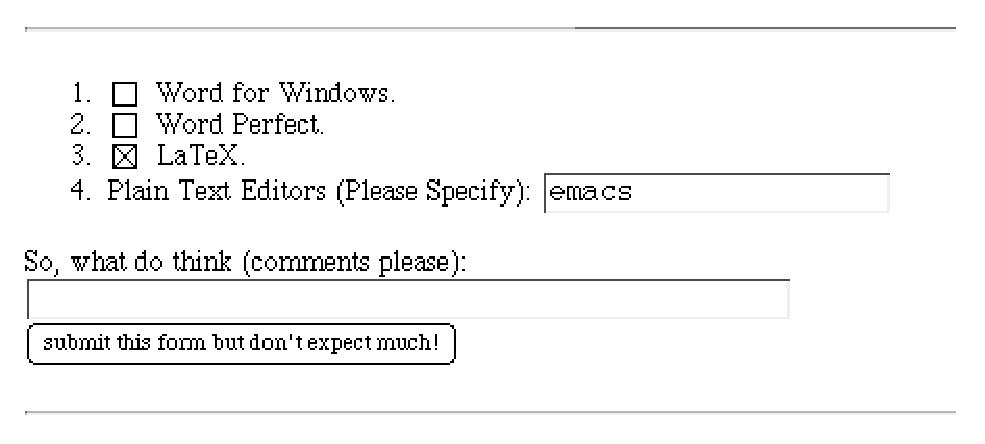
\includegraphics{psfiles/eform.ps}}}
    \end{center}
  \caption{An electronic form.
  In the online version the form would be active.}
  \label{eform}
\end{figure}
\end{latexonly}



\index{rawhtml@\Lc{rawhtml}}%
\paragraph*{\Lc{rawhtml}...\Lc{endrawhtml}\label{endrawhtml}}
\cbversion{97.1}\begin{changebar}
This is an alternative way to specify a chunk of raw \texttt{HTML} code,
using the old \AmS-style of delimiting environments.
Use of this style is discouraged; 
the \env{rawhtml} \htmlref{environment}{rawhtml} is preferred.%
\end{changebar}%

\index{comment@\env{comment} environment}%
\index{environment!comment@\env{comment}}%
\paragraph*{\Lc{begin\char123comment\char125}\label{comment}}
\cbversion{97.1}\begin{changebar}
This environment is simple for the convenience of ``commenting-out''
large sections of source code.
The contents of this environment is completely ignored,
both in the \LaTeX{} and \texttt{HTML} versions.
Such an environment is already used in \AmS-\LaTeX,
and perhaps with other packages.
It is defined here for its general utility.

\noindent
To insert \texttt{SGML}-style comments into the \texttt{HTML} files,
use the \env{rawhtml} environment as follows.
%begin{latexonly}
\begin{small}
%end{latexonly}
\begin{verbatim}
\begin{rawhtml}
<!--  this text is treated as a comment
      perhaps extending over several lines 
-->
\end{rawhtml}
\end{verbatim}
%begin{latexonly}
\end{small}
%end{latexonly}%
\end{changebar}%

\noindent
Note the \hyperref[page]{warning}{warning on page~}{}{env:warn}
concerning how the environment delimiters should be used in the
\LaTeX{} source code.


\index{latexonly@\Lc{latexonly}}%
\paragraph*{\Lc{comment...\char92endcomment}\label{endcomment}}
\cbversion{97.1}\begin{changebar}
This is an alternative way to specify a chunk of material intended
to be ignored in both the \LaTeX{} and \texttt{HTML} versions,
using the old \AmS-style of delimiting environments.
Use of this style (though convenient for typing) is discouraged,
since it is not as reliable as using the \env{comment} \htmlref{environment}{comment}.
\end{changebar}\html{\\}


\subsection{Arbitrary Tags and Attributes\label{sec:arbtags}}%
%\section{Arbitrary Tags and Attributes\label{sec:arbtags}}%
%
For version 97.1 of \latextohtml\ there is a new command which provides 
an extremely flexible way to include \texttt{HTML} 3.2 tags, along with
any values for the ``attributes'' of that tag, if desired.
\begin{quote}
\Lc{HTML}\verb|[|\Meta{attribs}\verb|]{|\Meta{tag}\verb|}|\label{HTMLtag}\\
\Lc{HTML}\verb|[|\Meta{attribs}\verb|]{|\Meta{tag}\verb|}{|\Meta{contents}\verb|}|
\end{quote}
When the \Meta{tag} also needs a closing tag (e.g \texttt{<I>...</I>})
the \Meta{contents} \emph{must} be given, enclosed in braces.
Both the opening and closing tags then will be placed correctly.


An important aspect of this is that any of the \Meta{tag},
\Meta{attribs} and \Meta{contents} may be given wholly
by expanding a \LaTeX{} macro, or may contain arbitrary macros, 
perhaps including other \Lc{HTML} commands.
\hyperref{The following table}{The contents of Figure~}{}{ex:HTML} 
was constructed using this feature; its \LaTeX{} source follows.

\HTML[50\% 3 noshade center]{HR}

\begin{htmlonly}
\begin{figure}
\begin{makeimage}
\end{makeimage}
\newcommand{\myalign}{center}
\newcommand{\mylist}{UL}
\newcommand{\myitem}[2]{\HTML[disc]{LI}{\simpletest{#1}{#2}}}
\newcommand{\simpletest}[2]{%
 \HTML{#1}{ a simple test of ``#2'',} using \HTML{CODE}{<#1>} .}
\newcommand{\tableopts}{10,border=5}

\newcommand{\tablelist}[4][\myalign]{\HTML[#1]{DIV}{
\HTML[\tableopts]{TABLE}{
\HTML[bottom]{CAPTION}{
#3
}\HTML{TR}{\HTML{TD}{
\HTML{#2}{
#4
}}}
}}\HTML[all]{BR}}

\tablelist[\myalign]{\mylist}{%
\textbf{A listing of the different text styles available in HTML 3.2}}{%
\myitem{B}{bold-face}
\myitem{I}{italics}
\myitem{TT}{teletype-text}
\myitem{U}{underlining}
\HTML[circle]{LI}{\simpletest{STRIKE}{strikeout}}
\myitem{EM}{emphasis style}
\myitem{STRONG}{strong style}
\myitem{CODE}{code style}
\myitem{CITE}{citation style}
\myitem{DFN}{definition style}
\HTML[square]{LI}{\simpletest{SAMP}{sample style}}
\HTML[square]{LI}{\simpletest{KBD}{keyboard style}}
\myitem{VAR}{variable style}}
%
 \caption{Example use of macros for raw \texttt{HTML} code.}
 \label{ex:HTML}
\end{figure}
\end{htmlonly}
%
\begin{latexonly}
\begin{figure}[ht]
\begin{center}
  \fbox{\scalebox{.7}{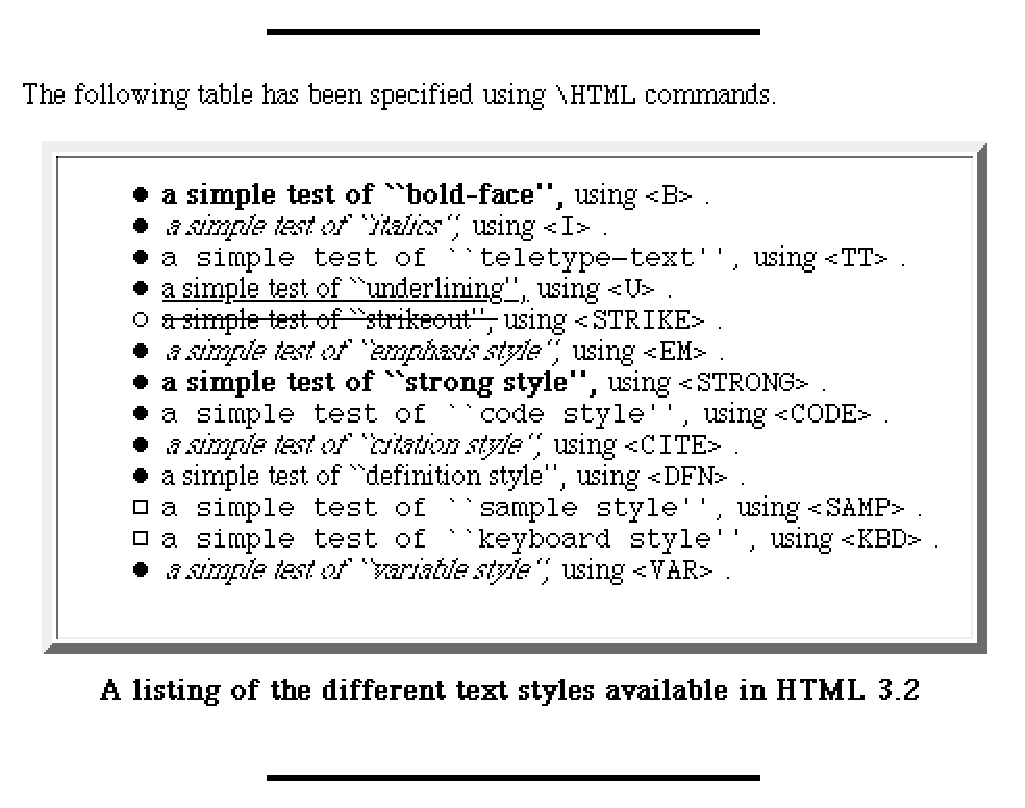
\includegraphics{psfiles/HTMLtab.ps}}}
 \caption{Example use of macros for raw \texttt{HTML} code.}
 \label{ex:HTML}
\end{center}
\end{figure}
\end{latexonly}

\HTML[50\% 3 noshade center]{HR}

%begin{latexonly}
\begin{small}
%end{latexonly}
\begin{verbatim}
\newcommand{\myalign}{center}
\newcommand{\mylist}{UL}
\newcommand{\myitem}[2]{\HTML[disc]{LI}{\simpletest{#1}{#2}}}
\newcommand{\simpletest}[2]{%
 \HTML{#1}{ a simple test of ``#2'',} using \HTML{CODE}{<#1>} .}
\newcommand{\tableopts}{10,border=5}

\newcommand{\tablelist}[4][left]{\HTML[#1]{DIV}{
\HTML[\tableopts]{TABLE}{
\HTML[bottom]{CAPTION}{
#3
}\HTML{TR}{\HTML{TD}{
\HTML{#2}{
#4
}}}
}}\HTML[all]{BR}}

\tablelist[\myalign]{\mylist}{%
\textbf{A listing of the different text styles available in HTML 3.2}}{%
\myitem{B}{bold-face}
\myitem{I}{italics}
\myitem{TT}{teletype-text}
\myitem{U}{underlining}
\HTML[circle]{LI}{\simpletest{STRIKE}{strikeout}}
\myitem{EM}{emphasis style}
\myitem{STRONG}{strong style}
\myitem{CODE}{code style}
\myitem{CITE}{citation style}
\myitem{DFN}{definition style}
\HTML[square]{LI}{\simpletest{SAMP}{sample style}}
\HTML[square]{LI}{\simpletest{KBD}{keyboard style}}
\myitem{VAR}{variable style}}
\end{verbatim}
%begin{latexonly}
\end{small}
%end{latexonly}

\HTML[50\% 3 noshade center]{HR}

\noindent
The above code demonstrates many aspects of the way \Lc{HTML}
commands can be used.
%
\begin{htmllist}\htmlitemmark{GreenBall}
\item [nesting: ] 
\Lc{HTML} commands can be nested to arbitrary depth.
%
\item [macros: ] 
Macros can be used to specify all or part of each argument.
%
\item [within macros: ] 
\Lc{HTML} commands work correctly within the expansions of other macros.
%
\item [attribute values: ]
Information within \Meta{attribs} can be specified in a very
loose way, as a comma-separated list of key/value pairs
or as single values. \\
Not even the commas are necessary: space(s), \Meta{tab}s 
or newlines are equally effective.
Indeed the horizontal rules preceding and following the table were 
specified by:
\begin{quote}
\begin{verbatim}
\HTML[50\% 3 noshade center]{HR}
\end{verbatim}
\end{quote}
%
\item [attribute names: ]
Usually it is \emph{not necessary} to know the names of the
attributes to the tags that are to be used. It is sufficient
just to give the values; these will be matched to the
appropriate attribute, according to the type of data required.
(If names are given, these are case-insensitive.)
%
\item [newlines: ] 
Although \LaTeX{} ignores linebreaks within the source code,
this is not so with \latextohtml. 
The strange spreading-out of the definition of the
\Lc{tablelist} command above was done with the purpose
solely of making the code in the resulting \texttt{HTML} files 
more easily readable, to a human.
(As most browsers ignore those newlines anyway, 
more compact code would have rendered the same on-screen.)
\end{htmllist}

\medskip\noindent
Some further aspects of the use of this \Lc{HTML}
command are not apparent from the above example. 

\begin{htmllist}\htmlitemmark{RedBall}
%
\item [invalid \Meta{tag}\,: ]
If a \Meta{tag} is specified that is not part of the 
\texttt{HTML} 3.2 specifications, then it and its attributes are 
not placed into the \texttt{HTML} document created by \latextohtml.
Any \Meta{contents} \emph{is} included as ordinary data; 
i.e. as text in paragraphs, etc.

\item [required attributes: ] 
Some tags have attributes which are required to have values,
if that tag is to be included in an \texttt{HTML} document.
Using the \Lc{HTML} command, if any such attribute
is not given an appropriate value then the tag is ignored.
Any \Meta{contents} are included in the document, 
as ordinary character data.

\item [valid HTML\,: ] 
Currently there is \emph{no} checking that the \Meta{contents}
of a \Meta{tag} contains only data (perhaps including other tags)
allowed by the DTD for \texttt{HTML} 3.2.
\begin{quote}
\textit{The requirement to produce valid \texttt{\upshape HTML} 
currently rests with the user.}
\end{quote}
This issue will be addressed in forthcoming revisions of \latextohtml.

\item [extra attributes and values: ]
The list of attributes for a \Meta{tag} can include
key-value pairs whose keys do not match any valid
attribute for the \Meta{tag}.
Such key-value pairs are simply ignored.
Similarly extra data values are ignored, 
as are values that do not match the
requirements for any valid attribute.

\item [attributes with similar data-types: ]
Several attributes to a \Meta{tag} may use values having 
the same or similar data-types. First any key-value pairs
are processed. Remaining values are allocated 
to those attributes which do not already have a value.
An ordering of the attributes is used, based on a perceived likelihood 
of each attribute being required to be changed from its default setting.

\end{htmllist}


\subsection{Conditional Text\label{sec:latexonly}}%
%\section{Conditional Text\label{sec:latexonly}}%
\tableofchildlinks*
\index{latexonly@\env{latexonly} environment}%
\index{htmlonly@\env{htmlonly} environment}%
\index{environment!htmlonly@\env{htmlonly}}%
\index{environment!latexonly@\env{latexonly}}%
\index{conditional text!scoped variant}\html{\\}%
\paragraph*{\Lc{begin\char123latexonly\char125} and 
\Lc{begin\char123htmlonly\char125}\label{latexonly}\label{htmlonly}}
Conditional text can be specified
using the environments \env{latexonly} and \env{htmlonly}. 
These allow writing parts of a document which are intended 
only for electronic delivery or only for paper-based delivery.

This would be useful for example in adding a long description of a
multi-media resource in the paper version of a document. 
Such a description would be redundant in the electronic version, 
as the user can have direct access to this resource. 

\medskip\goodbreak\noindent
Here is an example of the use of the \env{latexonly} environment,
used \hyperref[page]{earlier in}{on page~}{ of}{eform} this manual:
%begin{latexonly}
\begin{small}\indent
%end{latexonly}
\Lc{begin}\verb|{latexonly}|
\latex{\vskip-\baselineskip\vskip-\baselineskip}
\begin{verbatim}
\begin{figure}
    \begin{center}
    \fbox{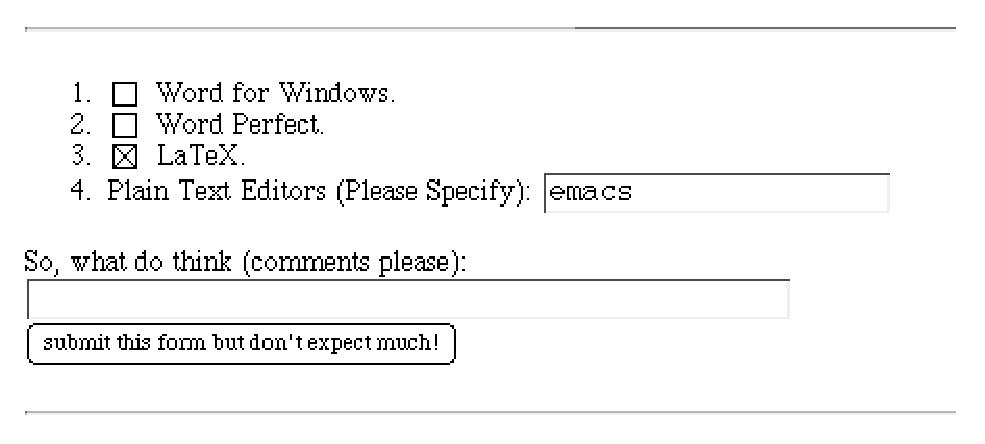
\includegraphics[width=4in]{psfiles/eform.ps}}
    \end{center}
    \caption{An electronic form. Of course in the online version of this
     document the form above would be active.}
\end{figure}
\end{verbatim}
\latex{\nobreak\vskip-\baselineskip\nobreak\indent\indent}%
\Lc{end}\verb|{latexonly}|
%begin{latexonly}
\end{small}\goodbreak\medskip
%end{latexonly}

\noindent
Note the \hyperref[page]{warning}{warning at the bottom of page~}{}{env:warn}
concerning how the environment delimiters should be used in the
\LaTeX{} source code.


\index{htmlonly@\Lc{htmlonly}}%
\paragraph*{\Lc{htmlonly...\char92endhtmlonly}\label{endhtmlonly}}
\cbversion{97.1}\begin{changebar}
This is an alternative way to specify a chunk of material intended
for the \texttt{HTML} version only,
using the old \AmS-style of delimiting environments.
Use of this style is discouraged; 
the \env{htmlonly} \htmlref{environment}{htmlonly} is preferred.%
\end{changebar}%


\index{latexonly@\Lc{latexonly}}%
\paragraph*{\Lc{latexonly...\char92endlatexonly}\label{endlatexonly}}
\cbversion{97.1}\begin{changebar}
This is an alternative way to specify a chunk of material intended
for the \LaTeX{} typeset version only,
using the old \AmS-style of delimiting environments.
Use of this style is discouraged; 
the \env{latexonly} \htmlref{environment}{latexonly} or the unscoped 
\htmlref{\texttt{\%begin\char123latexonly\char125}}{unlatexonly} 
construction are preferred.%
\end{changebar}%

\smallskip\noindent
Note the \hyperref[page]{warning}{warning at the bottom of page~}{}{env:warn}
concerning how the environment delimiters should be used in the
\LaTeX{} source code.


\index{conditional text!shorthand notation}%
\index{latex@\Lc{latex}}%
\index{html@\Lc{html}}%
\index{latexhtml@\Lc{latexhtml}}\html{\\}%
\paragraph*{\Lc{latex}, \Lc{html} and \Lc{latexhtml}\label{latexhtml}}
\cbversion{96.1}\begin{changebar}
There are also shorthand notations to accomplish the same thing 
as in the \env{latexonly} \htmlref{environment}{latexonly} and \env{htmlonly} 
\htmlref{environment}{htmlonly}, but with less typing.
\begin{itemize}
\item 
The \Lc{latex}\verb|{...}| command causes everything within the braces 
to be processed by \LaTeX, but ignored by \latextohtml.
\item  
Conversely, the \Lc{html}\verb|{...}| command causes everything within the braces 
to be ignored by \LaTeX{} and processed by \latextohtml.  
\item  
Finally the command \Lc{latexhtml}\verb|{...}{...}| causes everything 
within the first set of braces to be processed exclusively by \LaTeX, 
with the contents of the second set of braces processed solely by \latextohtml.%
\end{itemize}
\textbf{Warning: }
Only small pieces of text work reliably in this way. 
With whole paragraphs or contained sub-environments,
the ``conditional'' environments should be used instead.
\end{changebar}

\index{conditional text!without scope}%
\index{beginlatex@\texttt{\%{}begin\char123latexonly\char125}}%
\index{endlatex@\texttt{\%{}end\char123latexonly\char125}}%
\paragraph*{\texttt{\%begin\char123latexonly\char125}\label{unlatexonly}}
Another variant of the \env{latexonly} environment is available, 
in which everything between 
\verb|%|\verb|begin{latexonly}| and \verb|%|\verb|end{latexonly}| 
is ignored by \latextohtml.  
The difference is that the \env{latexonly} environment 
puts the contents into a group, in which all definitions are local.
There is no such scoping with the \verb|%begin...%end| variant,
since \LaTeX{} sees the initial \texttt{\%}s simply as starting comments.%

\medskip
\index{conditional text!example}\html{\\}\noindent
The following example should clarify what happens:
%begin{latexonly}
\begin{small}
%end{latexonly}
\begin{verbatim}
\newcommand{\A}{The letter A.}
\newcommand{\B}{The letter B.}
\end{verbatim}
\indent\indent\indent\verb|\|\verb|begin{latexonly}|\\
\indent\indent\verb|\renewcommand{\A}{Not the letter A.}|\\
\indent\indent\verb|\|\verb|end{latexonly}|\\
\indent\indent\verb|%|\verb|begin{latexonly}|\\
\indent\indent\verb|\renewcommand{\B}{Not the letter B.}|\\
\indent\indent\verb|%|\verb|end{latexonly}|
\begin{verbatim}
\begin{document}
\A \B
\end{document}
\end{verbatim}
%begin{latexonly}
\end{small}
%end{latexonly}
If you process this with \LaTeX, the result is: 
\quad\quad The letter A. Not the letter B.

\smallskip\noindent
Note the \hyperref[page]{warning}{warning at the bottom of page~}{}{env:warn}
concerning how the environment delimiters should be used in the
\LaTeX{} source code.

\medskip\index{conditional text!avoid using counters}\html{\\}\noindent
\textbf{Warning: }% 
Be careful when using \LaTeX{}  commands which alter the values of counters 
(e.g. numbered figures or equations) in conditional text, because this may 
cause the counter values in the electronic version to lose synchronisation 
with the values of the corresponding counters in the \LaTeX{} version.


\htmlrule[width=300]
\index{imagesonly@\env{imagesonly} environment}%
\index{environment!imagesonly@\env{imagesonly}}%
\paragraph*{\Lc{begin\char123imagesonly\char125}\label{imagesonly}}
\cbversion{97.1}\begin{changebar}
This environment is used to put \LaTeX{} code into the \fn{images.tex} file,
to be used when generating images. Typically this is used to add commands to
the preamble of \fn{images.tex}, such as setting the text or background color.
However code can be added at any other point as well; 
e.g. to change the background color of all images after a certain point in the document. 
\end{changebar}%

\smallskip\noindent
Note the \hyperref[page]{warning}{warning at the bottom of page~}{}{env:warn}
concerning how the environment delimiters should be used in the
\LaTeX{} source code.


\index{makeimage@\env{makeimage} environment}%
\index{environment!makeimage@\env{makeimage}}%
\paragraph*{\Lc{begin\char123makeimage\char125}\label{makeimage}}
\cbversion{97.1}\begin{changebar}
This is a special environment which forces an image to be made of its contents.
That is, one gets effectively a snapshot of a portion of a page
that has been typeset using \LaTeX. 
Within the normal \LaTeX{} typeset version of the document, this environment 
is completely transparent, adding its contents to the page as usual.

\index{makeimage@\env{makeimage} environment!inside@inside a \env{figure}}\html{\\}%
One further important use of the \env{makeimage} environment is as follows.
If a \env{makeimage} environment occurs as a sub-environment within 
a \env{figure} environment, then an image will \emph{not} be made of the
\env{figure}'s contents. Instead, the contents are treated as normal text,
each part being handled as if there were no \env{figure} at all,
except that everything is placed within a single cell of a
\HTMLtag{TABLE}...\HTMLtag{/TABLE} construction in \HTMLiii. 
The contents of any \Lc{caption}
commands are placed between \HTMLtag{CAPTION}...\HTMLtag{/CAPTION} tags 
for the \HTMLtag{TABLE}.

\index{makeimage@\env{makeimage} environment!empty sub-environment}\html{\\}%
Normally an image of the entire contents of the \env{figure} would be
placed within the single cell of the \HTMLtag{TABLE}.
Now images are made of any subparts of those \env{figure}'s contents 
that really need it, in particular the \env{makeimage} sub-environments.
An empty \env{makeimage} sub-environment does not generate an image of itself,
yet still it inhibits an image being made of the whole \env{figure}.
These comments apply also to \env{table} environments.
\end{changebar}\html{\\}




\subsection{Symbolic References shown as Hyperized Text\label{hyperized}%
%\section{Symbolic References shown as Hyperized Text\label{hyperized}%
\index{references@references\protect\label{IIIrefs}}}%
\tableofchildlinks*
\index{cross-references!|see{\htmlref{references}{IIIrefs}}}%
\index{references!symbolic\label{IIIsymref}}\index{symbolic labels|(}%
\index{references!numeric}%
\index{references!iconic}\html{\\}\noindent
In printed documents cross-references are shown 
through a \emph{numeric or symbolic indirection} 
e.g. ``see Figure 1'' (numeric indirection), 
or ``see section `Changes'~'' (symbolic indirection).  
\latextohtml{} can mirror this mechanism using the same numeric 
or symbolic references,
or when these are not appropriate by using iconic references.

\index{references!without indirection}%
\index{references!highlighted text}\html{\\}%
In a hypertext document however, cross-references can be shown 
without any indirection, just by highlighting a relevant piece of text. 
This can make a document more readable as it removes unnecessary
information. 

\index{hyperref@\Lc{hyperref}}%
\paragraph*{\Lc{hyperref}\label{hyperref}}
A single new \LaTeX{} command \Lc{hyperref} can be used for
specifying how a cross-reference should appear, 
both in the printed document and in the hypertext version.
For example, assuming that the label \verb|{sec:cond}|\label{sec:cond} 
is defined somewhere within a document, 
the command \Lc{hyperref}, taking 4 arguments,
can be used in that document as follows:
\index{hyperref@\Lc{hyperref}}%
\index{conditional text}%
%begin{latexonly}
\begin{small}
%end{latexonly}
\begin{verbatim}
\emph{Is the concept of
\hyperref
               % This will be highlighted in the hypertext version
{conditional text}			% argument #1
               % This will be shown in the printed version 
               % followed by a numeric reference ...      
{conditional text (see Section }  	% argument #2
               % ... followed by this text
{ for more information)} 		% argument #3
               % This is the common label 
{sec:cond}				% argument #4
a good idea? }
\end{verbatim}
%begin{latexonly}
\end{small}
%end{latexonly}

\noindent
Here is how it will be shown:
\begin{quote}
\emph{Is the concept of
\hyperref
% This will be highlighted in the hypertext version
{conditional text}
% This will be shown in the printed version  
% followed by a numeric reference ...      
{conditional text (see Section }  
% ... followed by this text
{ for more information)} 
% This the common label 
{sec:cond}
a good idea? }
\end{quote}

\begin{htmlonly}
In the printed version what would appear is:
\begin{quote}
\emph{Is the concept of conditional text (see Section 4.2 for more information) 
a good idea?}
\end{quote}
\end{htmlonly}

\begin{latexonly}%
In the hypertext version what would appear is:
\begin{quote}
\emph{Is the concept of \underline{conditional text} a good idea?}
\end{quote}
(Of course \underline{conditional text} would be an active hypertext link.)
\end{latexonly}

\bigskip\htmlrule[50\% center]
\cbversion{97.1}\begin{changebar}%
\noindent
An extended syntax for \Lc{hyperref} uses an optional argument, 
which determines what information is to be placed in the \LaTeX{} version
of the document. The value of this optional argument can also affect 
the number of required arguments. 
These forms are recognised:

%begin{latexonly}
\begin{small}
%end{latexonly}
\begin{quote}\label{hypernoref}
\Lc{hyperref}\verb|[ref]{|\Meta{HTML-text}\verb|}{|\Meta{LaTeX-text}%
\verb|}{|\Meta{post-LaTeX}\verb|}{|\Meta{label}\verb|}|\\
\Lc{hyperref}\verb|{|\Meta{HTML-text}\verb|}{|\Meta{LaTeX-text}%
\verb|}{|\Meta{post-LaTeX}\verb|}{|\Meta{label}\verb|}|\medskip

\Lc{hyperref}\verb|[pageref]{|\Meta{HTML-text}\verb|}{|\Meta{LaTeX-text}%
\verb|}{|\Meta{post-LaTeX}\verb|}{|\Meta{label}\verb|}|\\
\Lc{hyperref}\verb|[page]{|\Meta{HTML-text}\verb|}{|\Meta{LaTeX-text}%
\verb|}{|\Meta{post-LaTeX}\verb|}{|\Meta{label}\verb|}|\medskip

\Lc{hyperref}\verb|[noref]{|\Meta{HTML-text}\verb|}{|\Meta{LaTeX-text}%
\verb|}{|\Meta{label}\verb|}|\\
\Lc{hyperref}\verb|[no]{|\Meta{HTML-text}\verb|}{|\Meta{LaTeX-text}%
\verb|}{|\Meta{label}\verb|}|
\end{quote}
%begin{latexonly}
\end{small}
%end{latexonly}

\noindent
The first two are the defaults, where \LaTeX{} 
uses \Lc{ref}\verb|{|\Meta{label}\verb|}|.
With the next two \LaTeX{} uses \Lc{pageref}\verb|{|\Meta{label}\verb|}|,
while with the final two \LaTeX{} completely ignores the \Meta{label},
setting just the \Meta{LaTeX-text}.
\end{changebar}

\medskip
\index{hyperref@\Lc{hyperref}!pageref@\Lc{pageref} example}%
\html{\\}\noindent
For creating hyperlinks to other documents
using symbolic reference \Meta{label}s, 
see also the \Lc{externalref} 
\hyperref[page]{command}{command, described on page~}{}{externref}.

\medskip\noindent
The preceding paragraph is an example of the use of the \Lc{hyperref[page]} option.
Its source code is:
%begin{latexonly}
\begin{small}
%end{latexonly}
\begin{verbatim}
For creating hyperlinks to other documents
using symbolic reference \Meta{label}s, 
see also the \Lc{externalref} 
\hyperref[page]{command}{command, described on page~}{}{externref}.
\end{verbatim}
%begin{latexonly}
\end{small}
%end{latexonly}
\begin{htmlonly}
which appears in the \LaTeX{} typeset version as:
\begin{quote}
For creating hyperlinks to other documents
using symbolic reference \Meta{label}s, see also the
\Lc{externalref} command, described on page~31.
\end{quote}
\end{htmlonly}
\begin{latexonly}
which appears in the \texttt{HTML} version as:
\begin{quote}
For creating hyperlinks to other documents, using symbolic reference \Meta{label}s, 
see also the \Lc{externalref} \underline{command}.
\end{quote}
with the \underline{command} being an active hyperlink.
\end{latexonly}
\smallskip\noindent
In fact both \Lc{hyperref} and the \Lc{htmlref} command, to be described next,
permit textual hyperlinks based on symbolic \Meta{label}s from external files.


\index{htmlref@\Lc{htmlref}}%
\index{html.sty@\texttt{html.sty} style-file}
\paragraph*{\Lc{htmlref}\label{htmlref}}
Another command also defined in \fn{html.sty} is \Lc{htmlref} 
which has the same effect as \Lc{hyperref}
during the conversion to \texttt{HTML}.
It takes two arguments, some text and a label. 
In the \texttt{HTML} version the
text will be ``hyperized'', pointing to the label. 
In the paper version the text will be shown as it is 
and the label will be ignored; e.g.
%
\index{htmlref@\Lc{htmlref}!easy to make links}%
%begin{latexonly}
\begin{small}
%end{latexonly}
\begin{verbatim}
With \verb|\htmlref| \htmlref{it's easy to make links}{fig:example}.
\end{verbatim}
%begin{latexonly}
\end{small}
%end{latexonly}
which produces:
\begin{quote}
With \Lc{htmlref} \htmlref{it's easy to make links}{fig:example}.
\end{quote}
\begin{htmlonly}
In the \LaTeX{} typeset version it will appear simply as:
\begin{quote}
With \Lc{htmlref} it's easy to make links.
\end{quote}
\end{htmlonly}
\begin{latexonly}
In the \texttt{HTML} version it is shown as:
\begin{quote}
With \Lc{htmlref} \underline{it's easy to make links}.
\end{quote}
\end{latexonly}
\html{\\}
\goodbreak

\subsection{Hypertext Links in Bibliographic References (Citations)}%
%\section{Hypertext Links in Bibliographic References (Citations)}%
\tableofchildlinks*
\index{references!bibliographic}\index{bibliography|(}%
\index{bibliography!bibliographic database}%
\index{bibliography!using .bib@using \texttt{.bib} file}\html{\\}%
If a report or a book that is cited (using the \Lc{cite} command) 
is available (or there is information about it) on the World-Wide
Web, then it is possible to add the appropriate hypertext links
in your bibliographic database (the \texttt{.bib}) file. 

\bigskip
\index{bibliography!example using URLs}%
\index{bibliography!string commands@\texttt{\char64 string} commands}%
\index{LaTeX blue book@\LaTeX{} blue book}\html{\\}%
\noindent
Here is an example of a bibliographic entry for the original
\LaTeX{} \cite{lamp:latex} blue book:\nobreak
%begin{latexonly}
\begin{small}
%end{latexonly}
\begin{verbatim}
@string{curiaURL="\htmladdnormallink
{http://curia.ucc.ie/info/TeX/menu.html}
{http://curia.ucc.ie/info/TeX/menu.html}"}

@string{fernURL="\htmladdnormallink
{http://es-sun2.fernuni-hagen.de/info2html?(latex.info)Top}
{http://es-sun2.fernuni-hagen.de/info2html?(latex.info)Top}"}

@book{lamp:latex,
title = "LaTeX User's Guide \& Reference Manual, 2nd edition",
year = 1994 ,
author = "Leslie Lamport",
Publisher = "Addison--Wesley Publishing Company, Inc.",
note = "Online information on {\TeX} and {\LaTeX} is available at "
 # curiaURL # " and " # fernURL }
\end{verbatim}
%begin{latexonly}
\end{small}
%end{latexonly}
See the \htmlref{bibliography}{biblio} for how this will appear.\html{\\}
No other modifications are required; \LaTeX{} and Bib\TeX{} should work as normal.
%
\index{bibliography!string commands@\texttt{\char64string} commands}%
\cbversion{96.1f}\begin{changebar}
Note that it would be sensible to put the \texttt{@string} commands
into a separate file, \fn{urls.bib} say, 
loaded with the main file via\html{\\} \verb|\bibliography{urls,...}|.%
\end{changebar}

\smallskip\index{citations!Harvard style}%
\index{bibliography!Harvard style}\label{harvard}\html{\\}%
\noindent
For those who use the Harvard style for references
\htmladdnormallinkfoot{there exists a special conversion add-on package}%
{http://www.arch.su.edu.au/\~{}peterw/latex/harvard/}.

\index{citations!natbib@\env{natbib} package}%
\index{bibliography!natbib@\env{natbib} package}%
\index{citations!Harvard style!handled@handled by \env{natbib}}%
\cbversion{96.1g}\begin{changebar}
The \env{natbib} package, written for \LaTeX{} by \PatrickDaly,
provides even more flexibility in the way a reference may be cited. 
All the features of \htmlref{this package}{natbib} are implemented 
for \latextohtml{} via the \fn{natbib.perl} file.
(Indeed there is even a mode whereby \env{natbib} handles
the Harvard style of citation. 
This requires loading also the \env{nharvard} \htmlref{package}{nharvard}.)

\medskip
\noindent\textbf{Thanks...} to \Wilck\ for the bulk of the work 
in producing this extension, and to \RossMoore\ for 
necessary adjustments to allow it to work correctly with the 
\htmlref{document segmentation strategy}{Segmentation}.
\end{changebar}


\index{hypercite@\Lc{hypercite}}%
\paragraph*{\Lc{hypercite}\label{hypercite}}
\cbversion{97.1}\begin{changebar}
Analogous to \Lc{hyperref} is the \Lc{hypercite} command,
which allows a free-form textual hyperlink to the bibliography,
whereas the \LaTeX{} typeset version contains the usual citation code.
The allowed syntax is as follows.
%begin{latexonly}
\begin{small}
%end{latexonly}
\begin{quote}
\Lc{hypercite}\verb|[int]{|\Meta{HTML-text}\verb|}{|\Meta{LaTeX-text}%
\verb|}{|\Meta{opt-LaTeX}\verb|}{|\Meta{label}\verb|}|\\
\Lc{hypercite}\verb|[cite]{|\Meta{HTML-text}\verb|}{|\Meta{LaTeX-text}%
\verb|}{|\Meta{opt-LaTeX}\verb|}{|\Meta{label}\verb|}|\\
\Lc{hypercite}\Meta{HTML-text}\verb|}{|\Meta{LaTeX-text}%
\verb|}{|\Meta{opt-LaTeX}\verb|}{|\Meta{label}\verb|}|\medskip

\Lc{hypercite}\verb|[nocite]{|\Meta{HTML-text}\verb|}{|\Meta{LaTeX-text}%
\verb|}{|\Meta{label}\verb|}|\\
\Lc{hypercite}\verb|[no]{|\Meta{HTML-text}\verb|}{|\Meta{LaTeX-text}%
\verb|}{|\Meta{label}\verb|}|\\
\Lc{hypercite}\verb|[ext]{|\Meta{HTML-text}\verb|}{|\Meta{LaTeX-text}%
\verb|}{|\Meta{label}\verb|}|
\end{quote}
%begin{latexonly}
\end{small}
%end{latexonly}
The first three forms are equivalent; 
\LaTeX{} uses \Lc{cite}\verb|[|\Meta{opt-LaTeX}\verb|]|\Meta{label}\,,
after placing the \Meta{LaTeX-text}.
Note that \verb|{|\Meta{opt-LaTeX}\verb|}| \emph{must} be specified, 
even if empty `\verb|{}|'.

Similarly the latter three forms are equivalent, 
with \LaTeX{} using \Lc{nocite}\verb|{|\Meta{label}\verb|}|\,, 
to force the particular reference to appear on the bibliography page, 
even though no explicit marker is placed at this point.
(Thus there is no need for an optional  \Meta{opt-LaTeX} argument.)\html{\\}
Within the \texttt{HTML} version a hyperlink is produced when the \Meta{HTML-text} 
is not empty. External label files are also searched, 
in order to match the symbolic \Meta{label}, see also 
\hyperref[page]{\Lc{externalcite}}{\Lc{externalcite} on page~}{}{externcite}.

\smallskip\noindent\label{hyperciteXmpl}%
\index{hypercite@\Lc{hypercite}!example}%
\index{htmlcite@\Lc{htmlcite}!example}\html{\\}\noindent
\htmlref{Earlier}{hypcites} in this manual the following source code was used:
%begin{latexonly}
\begin{small}
%end{latexonly}
\begin{verbatim}
commands described in the \LaTeX{} \htmlcite{blue book}{lamp:latex}, 
...
as well as many other \LaTeX{} constructions, such as are described in 
the \LaTeX{} \hypercite{\emph{Companion}}{\emph{Companion}}{}{goossens:latex} 
and \LaTeX{} \hypercite{\emph{Graphics Companion} (e.g. \Xy-pic)}%
{\emph{Graphics Companion}}{\Xy-pic}{goossens:latexGraphics};
\end{verbatim}
%begin{latexonly}
\end{small}
%end{latexonly}
which produces:
\begin{quote}
commands described in the \LaTeX{} \htmlcite{blue book}{lamp:latex}, 
\\~~...\\
as well as many other \LaTeX{} constructions, such as are described in 
the \LaTeX{} \hypercite{\emph{Companion}}{\emph{Companion}}{}{goossens:latex} 
and \LaTeX{} \hypercite{\emph{Graphics Companion} (e.g. \Xy-pic)}%
{\emph{Graphics Companion}}{\Xy-pic}{goossens:latexGraphics};
\end{quote}
\begin{latexonly}
whereas in the \texttt{HTML} version one sees:
\begin{quote}
commands described in the \LaTeX{} \underline{blue book}, 
\\~~...\\
as well as many other \LaTeX{} constructions, 
such as are described in the \LaTeX{} \underline{\emph{Companion}} 
and  \LaTeX{} \underline{\emph{Graphics Companion} (e.g. \Xy-pic)};
\end{quote}
\end{latexonly}
%
\begin{htmlonly}
whereas in the \LaTeX{} typeset version one sees:
\begin{quote}
commands described in the \LaTeX{} blue book,\\
~~...\\
as well as many other \LaTeX{} constructions, such as are described in the \LaTeX{} 
\textit{Companion}[2] and \LaTeX{} \textit{Graphics Companion}[3, \Xy-pic];
\end{quote}
\end{htmlonly}
\end{changebar}%


\index{htmlcite@\Lc{htmlcite}}%
\paragraph*{\Lc{htmlcite}\label{htmlcite}}
\cbversion{97.1}\begin{changebar}
Analogous to \Lc{htmlref} is the \Lc{htmlcite} command,
which creates a textual hyperlink to a place on the document's bibliography page, 
but without displaying any reference marker in the \LaTeX{} typeset version.
(See \htmlref{above}{hyperciteXmpl} for an example.)%

The \Lc{externalcite} 
\hyperref[page]{command}{command, described on page~}{, }{externcite}
provides a similar facility when the bibliography page is ``external'';
that is, not part of the current document.%
\end{changebar}

\index{bibliography|)}



\subsection{Symbolic References between Living Documents\label{external_cross}}%
%\section{Symbolic References between Living Documents\label{external_cross}}%
\tableofchildlinks*
\index{external references|(}
\index{references!to external documents}%
\index{references!symbolic}%
\index{symbolic labels!see also@\emph{see also} 
 \htmlref{references, symbolic}{IIIsymref}}%
\index{labels!symbolic}%
%
\cbversion{96.1}\begin{changebar}
The method of the previous section to generated
symbolic \htmlref{hyperized}{hyperized} links can
easily be extended to \emph{external} documents processed by \latextohtml.  
When \latextohtml{} processes a document, it generates a \Perl{} file 
named \Meta{prefix}\fn{labels.pl}
which contains a list of all the symbolic labels that were defined, 
along with their locations.  
The \htmlref{\Meta{prefix}}{prefix} is empty unless otherwise specified, 
to allow different document segments to share the same directory.  
\end{changebar}

\index{externallabels@\Lc{externallabels}}%
\index{externalref@\Lc{externalref}}%
\paragraph*{\Lc{externallabels}\label{externlabels}}
\cbversion{96.1}\begin{changebar}
Links to an external document are then possible once a connection 
is established to that document's \fn{labels.pl} file.  
This connection is established by the \Lc{externallabels} command:%
\end{changebar}%
%
\begin{quote}
%begin{latexonly}
\begin{small}
%end{latexonly}
\Lc{externallabels}\verb|{|\Meta{URL to directory of external document}\verb|}|\\
\verb|               {|\Meta{local copy of external document labels.pl file}\verb|}|
%begin{latexonly}
\end{small}
%end{latexonly}
\end{quote}
%
\index{labels!external}\html{\\}%
The first argument to \Lc{externallabels} should be a URL to 
the directory containing the external document.  
The second argument
should be the full path-name to the \fn{labels.pl} file belonging
to the external document.  Note that for \emph{remote} external documents
it is necessary to copy the \fn{labels.pl} file locally so that it
can be read when processing a local document that uses it.
The command \Lc{externallabels} can be used once for each external
document in order to import the \textit{external labels}\label{externallabels}
into the current document.
A warning is given if \fn{labels.pl} cannot be found.

\begin{changebar}%
If a symbolic reference made in either of the commands described
\hyperref{on the previous page}{in Section~}{}{hyperized} is not 
defined within the document itself,
\latextohtml{} will look for that reference in one of the external
files\footnote{Care must be taken to ensure that critical symbolic
references are unique across related documents.}.
After any modifications in an external document 
(sections added/deleted, segmentation into different physical parts, etc.) 
a new \fn{labels.pl} will be generated.  
If the \Lc{externallabels} command in another 
document contains the correct address to an updated copy of
the \fn{labels.pl} file, then the cross-references will be re-aligned
after running the local document through the translator.

\index{labels!internal}\label{internallabels}\html{\\}%
There is also a mechanism analogous to the
\textit{label--ref} pairs of \LaTeX, which can be used only 
within a single document. 
These labels are called \textit{internal labels},
as opposed to the \htmlref{external labels}{externallabels} defined above.
They are used extensively with the document segmentation strategy
described \hyperref{later}{in Section~}{}{Segmentation}.

Either type of label is defined with a \LaTeX{} \Lc{label} command.  
Labels can be referenced \textit{within} a document using a \Lc{ref} command.
When processed by \LaTeX, each \Lc{ref} command is replaced by the 
section number in which the corresponding \Lc{label} occurred.
When processed by the translator, each \Lc{ref} is replaced by 
a hypertext link to the place where the corresponding \Lc{label} occurred.%
\end{changebar}%
 

\index{references!to external documents}%
\index{externalref@\Lc{externalref}}%
\paragraph*{\Lc{externalref}\label{externref}}
\begin{changebar}%
This mechanism can be extended to external documents:
\begin{quote}
%begin{latexonly}
\begin{small}
%end{latexonly}
\Lc{externalref}\verb|{|\Meta{symbolic label in remote document}\verb|}|
%begin{latexonly}
\end{small}
%end{latexonly}
\end{quote}
The argument to \Lc{externalref} may be any symbolic label defined 
in the \fn{labels.pl} file of any of the external documents.
Such references to external symbolic labels are then translated
into hyper-links pointing to the external document.%
\end{changebar}%


\index{citations!within external bibliographies}%
\index{externalcite@\Lc{externalcite}}%
\paragraph*{\Lc{externalcite}\label{externcite}}
\cbversion{97.1}\begin{changebar}
%
Analogous to \htmlref{\Lc{externalref}}{externref},
the \Lc{externalcite} command is used to create a citation link,
where the bibliography page is not part of the current document.
As with \Lc{externalref} symbolic labels for the bibliography page
must have been loaded using 
\htmlref{\Lc{externallabels}}{externlabels}.

A particularly important use for this is in allowing multiple documents 
to access information in a common bibliographic listing.
For example: all of an author's publications; 
a comprehensive listing of publications in a particular field; 
the (perhaps yearly) output of publications 
from a particular organisation or institution.

\medskip\noindent
\textbf{Thanks...} to \Engberg\ for suggesting this feature.
\end{changebar}

\index{external references|)}


\subsubsection{Cross-Referencing Example\label{crossrefs}}% 
%\subsection{Cross-Referencing Example\label{crossrefs}}% 
To understand this mechanism better consider 
how you would maintain a link to this section  
(of the hypertext version of this document) from one of your documents,
without using labels.
Sure enough you can get the name of the physical file that this section is in. 
This however is quite likely to change, and any links to it would become invalid. 
\index{link validation!done by hand}%
To update your link, the name of the new file must be found 
and your link changed by hand. 
Also there is no general updating mechanism, so the only way to find
out if your document is pointing to the right place is by actually
following the link, then doing a manual update\footnote{%
Link validation can be done automatically but the updating must be done
manually when filenames have changed (assuming no other symbolic label
mechanism is available).}.

\index{link validation!symbolic labels}\html{\\}%
Next consider how it could be done with symbolic labels. 
First you have to import the labels used in this document 
by copying the file \htmladdnormallink{\fn{labels.pl}}
{http://cbl.leeds.ac.uk/nikos/tex2html/doc/manual/labels.pl},
saving it in \path{/tmp/labels.pl} say,
then adding anywhere in your document:
%begin{latexonly}
\begin{small}
%end{latexonly}
\begin{verbatim}
\externallabels{http://cbl.leeds.ac.uk/nikos/tex2html/doc/manual}%
               {/tmp/labels.pl}
\end{verbatim}
%begin{latexonly}
\end{small}
%end{latexonly}
After that you can use the label `\texttt{crossrefs}' defined at the beginning of this 
section\footnote{You either have to guess the role of each label by
looking at the \fn{labels.pl} file or by asking the author!} as follows:
%begin{latexonly}
\begin{small}
%end{latexonly}
\begin{verbatim}
\externalref{crossrefs}
\end{verbatim}
%begin{latexonly}
\end{small}
%end{latexonly}
This will be translated into the appropriate hyper-link to this page.
If there are any changes in this document and you would like to
bring your document up-to date, you have to copy 
\htmladdnormallink{\fn{labels.pl}}%
{http://cbl.leeds.ac.uk/nikos/tex2html/doc/manual/labels.pl} again
and rerun the translator on your document. Of course if I move the 
directory containing the \texttt{HTML} files for this document somewhere else, 
then you would have to make a change in the argument of the 
\Lc{externallabels} command to reflect this. 

\index{references!collaboration required}%
It is obvious that some level of collaboration is required between
authors trying to maintain cross-references between different documents. 
Using symbolic labels makes this a lot easier 
(especially for documents written by the same author).
\index{symbolic labels|)}



\subsection{Miscellaneous commands for \texttt{HTML} effects\label{misceffects}}%
%\section{Miscellaneous commands for \texttt{HTML} effects\label{misceffects}}%
\tableofchildlinks*
\index{html.sty@\texttt{html.sty} style-file}%

\noindent
The \env{html} package, through the \LaTeX{} input file \fn{html.sty},
and its \Perl{} counterpart \fn{html.perl}, implements several 
new commands that are intended entirely for effects within the
produced \texttt{HTML} files. In \LaTeX{} these commands, their arguments,
and any optional arguments are completely ignored.

\index{htmlrule@\Lc{htmlrule}}%
\index{visual separation!using \Lc{htmlrule}}%
\paragraph*{\Lc{htmlrule } and 
 \Lc{htmlrule*}\label{htmlrule}}
One such device provided by \fn{html.sty},
is the \Lc{htmlrule} command. 
This puts a horizontal rule into the \texttt{HTML} file only;
being ignored in the \texttt{.dvi} version. 
It is useful to provide extra visual separation between paragraphs,
without creating a new \texttt{HTML} page, 
such as might warrant extra vertical space within the printed version.

\index{htmlrule!htmlrulestar@\Lc{htmlrule*}}%
\index{htmlrule!variants}%
\index{htmlrule!attributes@attributes to the \HTMLtag{HR} tag}%
\cbversion{97.1}\begin{changebar}
Much variation can be obtained in the horizontal rule that is produced,
using extended forms of the \Lc{htmlrule} command:
\begin{quote}
%begin{latexonly}
\begin{small}
%end{latexonly}
\Lc{htmlrule}\\
\Lc{htmlrule*}\\
\Lc{htmlrule[}\Meta{attribs}\texttt{]}\\
\Lc{htmlrule*[}\Meta{attribs}\texttt{]}
%begin{latexonly}
\end{small}
%end{latexonly}
\end{quote}
Whereas a ``break'' tag \HTMLtag{BR} normally precedes the \HTMLtag{HR} generated
by the \Lc{htmlrule} command, 
this break is omitted when using the \Lc{htmlrule*} variant. 

\htmlrule[center,width=200]

\noindent
Furthermore, the optional argument \Meta{attribs} can be used to specify 
attributes for \emph{both} the \HTMLtag{HR} and \HTMLtag{BR} tags. 
More specifically, \Meta{attribs} should be a list of attribute-names 
and/or key-value pairs \texttt{\Meta{key}=\Meta{value}} separated by spaces or commas. 
This list is parsed to extract those attributes applicable to the \HTMLtag{HR} tag,
and those applicable to the \HTMLtag{BR} (with the unstarred variant).

\medskip\htmlrule[right,width=200,size=5]
\noindent
Using \HTMLiii, this allows variations to be specified for:
\begin{itemize}
\item 
the (vertical) thickness of the horizontal line in pixels: \texttt{SIZE=\Meta{num}};
\item 
the (horizontal) width of the line in pixels or points: \texttt{WIDTH=\Meta{width}};
\item 
alignment: \texttt{WIDTH=\char34...\char34 } 
taking \texttt{left}, \texttt{right} or \texttt{center};
\item 
removal of the shadowed effect \texttt{NOSHADE};
\item 
positioning of the rule with respect to text-flows: 
\texttt{CLEAR=\char34...\char34 } 
taking \texttt{left}, \texttt{all}, \texttt{right} or \texttt{none}. 
\htmlrule[right,width=200,size=5]
\end{itemize}%
Some examples of these effects appear on 
\latex{the \texttt{HTML} version of} this page.%
\end{changebar}%


\index{strikeout@\Lc{strikeout}}%
\paragraph*{\Lc{strikeout\char123}\Meta{text}\texttt{\char125}\label{strikeout}}
\cbversion{97.1}\begin{changebar}
With this command the \Meta{text} is processed as normal in the \texttt{HTML} version,
then placed between \HTMLtag{STRIKE}...\HTMLtag{/STRIKE} tags.
Thus a horizontal line should be drawn through the middle of the \Meta{text}.\html{\\}
Currently the command and the \Meta{text} are ignored in the \LaTeX{} version.%
\end{changebar}%


\index{tableofchildlinks@\Lc{tableofchildlinks}}%
\paragraph*{\Lc{tableofchildlinks }\label{tochlinks}}
\cbversion{97.1}\begin{changebar}
As an extra aid to navigation within a long page, 
containing several (sub)subsections or deeper levels of sectioning,
there is the \Lc{tableofchildlinks} command.
This does not generate anything new, for a table of the child links
on or from a page is generated automatically by \latextohtml.

However if this command, or its variant \Lc{tableofchildlinks*},
occurs within the source code to appear on a particular \texttt{HTML} page,
then the child-links table will be placed at that point
where the command occurs. 
Normally a break tag \HTMLtag{BR} is inserted to separate the table of child-links 
from the surrounding text. The \Lc{tableofchildlinks*} omits this extra break
when it would result in too much space above the table.

For example throughout this section of the \latex{\texttt{HTML} version of the }manual, 
all subsections in which several explicit commands have been discussed
have their child-links table placed at the top of the page,
using \Lc{tableofchildlinks*}. 
This helps to quickly find the description of how the commands are used.%
\end{changebar}%


\index{htmlinfo@\Lc{htmlinfo}}%
\paragraph*{\Lc{htmlinfo }\label{htmlinfo}}
\cbversion{97.1}\begin{changebar}
Normally an ``About this document...'' page is created at the end
of the \texttt{HTML} document, containing technical information
about how the document was created, by whom, or any other information
contained in the \fn{\$INFO} \htmlref{variable}{infostring}.
This information can be made to appear at any other place within the document 
by specifying \Lc{htmlinfo} at the desired place in the source.
For example, the information may be best suited for the title-page.

The variant \Lc{htmlinfo*} places the information, but leaves out the 
standard ``About this document...'' header. 
Instead the \htmlref{\Lc{htmlhead}}{htmlhead} command 
can be used to place an alternative heading, prior to the \Lc{htmlinfo*} command.
Neither this heading nor the \fn{\$INFO} \htmlref{contents}{infostring} appears 
in the \LaTeX{} typeset version.%
\end{changebar}%


\index{bodytext@\Lc{bodytext}}%
\paragraph*{\Lc{bodytext\char123}\Meta{options}\texttt{\char125}\label{bodytext}}
\cbversion{96.1g}\begin{changebar}
The text and background colors, and colors for the text of hypertext links can
be set on an \texttt{HTML} page by giving appropriate attributes 
with the \HTMLtag{BODY ...} tag. This is particularly easy to do
using the \Lc{bodytext} command, 
which simply inserts the \Meta{code} as the desired list of attributes.%

\medskip
\index{bodytext@\Lc{bodytext}!no checking for valid attributes}\html{\\}%
\noindent
\textbf{Warning: }Any previous settings for the \HTMLtag{BODY ...} tag
are discarded. Furthermore no checking is done to verify whether the given \Meta{options}
indeed contains a list of attributes and values valid for the \HTMLtag{BODY ...} tag.\html{\\}
When using \Lc{bodytext} you are assumed to know precisely what you are doing!

\medskip\noindent
Other packages contain commands which alter the contents of the \HTMLtag{BODY ...} tag;
notably the \fn{color.perl} implementation of \LaTeX's \env{color} package,
and the (prototype) \env{frames} package, by \Wilck\ and \RossMoore.
In both these packages the requested information is checked for
validity as an attribute within the \HTMLtag{BODY ...} tag.
\end{changebar}%

\index{htmlbody@\Lc{htmlbody}}%
\paragraph*{\Lc{htmlbody\char123}\Meta{options}\texttt{\char125}\label{htmlbody}}
\cbversion{97.1}\begin{changebar}
This is similar to the \Lc{bodytext} command, except that it adds the
value of an attribute, or allows an existing value to be changed.
Thus it can be used to alter just a single one of the text and background colors, 
colors for the text of hypertext links or add a background pattern.
The \Meta{options} are given as key-value pairs; some checking is done to ensure 
the validity of the attributes whose values are being set.%
\end{changebar}%

\index{htmlbase@\Lc{htmlbase}}%
\paragraph*{\Lc{htmlbase\char123}\Meta{URL}\texttt{\char125}\label{htmlbase}}
\cbversion{96.1g}\begin{changebar}
This specifies that the given \Meta{URL} be included in the \HTMLtag{HEAD} section
of each \texttt{HTML} page via a tag: 
\texttt{<BASE HREF=\char34\Meta{URL}\char34}.\html{\\}
Such a feature is particularly useful\dots 
\begin{itemize}
\item
when preparing a document whose final location may be different from where it was created; 
By making all internal references be relative (to the the provided \Meta{URL}),
a whole directory tree containing the document 
and all its subparts can be moved to elsewhere.
A single edit in each \texttt{HTML} file produces the complete document intact 
at the new location.
%
\item
by allowing just single page to be copied to another location, but act as if it were
part of the original document (provided this is accessible across the Web).
Relative URLs within the copied page are relative to the base \Meta{URL},
rather than relative to the new location.
%
\item
Other uses for this feature are likely to become apparent.%
\end{itemize}\end{changebar}%


\index{HTMLset@\Lc{HTMLset}!alters a \Perl{} variable}%
\index{HTMLset@\Lc{HTMLsetenv}!alters a \Perl{} variable}%
\paragraph*{\Lc{HTMLset\char123}\Meta{which}\texttt{\char125\char123}%
\Meta{value}\texttt{\char125} and 
\Lc{HTMLsetenv\char123}\Meta{which}\texttt{\char125\char123}%
\Meta{value}\texttt{\char125}\label{HTMLset}}
\cbversion{97.1}\begin{changebar}
The \Lc{HTMLset} command provides a mechanism whereby an arbitrary
\Perl{} variable can be assigned a value dynamically, during the \latextohtml{} processing. 
A variable having name `\texttt{\$}\Meta{which}' is assigned the specified \Meta{value},
overwriting any value that may exist already. The \Lc{HTMLsetenv} is for the same purpose,
but it is expanded in order as if it were an environment, rather than a command.

\medskip\noindent
\textbf{Warning: }This is intended for \Perl{} programmers only.
Use this command at your own risk!
\end{changebar}

\htmlrule[width=300]
\index{LaTeX2HTML@\latextohtml{}!command for its name}%
\index{names of important packages}%
\index{latextohtml@\Lc{latextohtml}!gives @gives \latextohtml{}}%
\paragraph*{\Lc{latextohtml}\label{l2hname}} 
\cbversion{97.1}\begin{changebar}
expands to the name \latextohtml, of this translator.
Commands for parts of names of important \LaTeX{} packages are also 
included with \latextohtml: e.g. \TeX, \LaTeX, \AmS, \Xy\,.
(This is to make it easy to refer to these products, in a consistent way
within the \texttt{HTML} pages; you may still need \LaTeX{} definitions
for the typeset version.)
\end{changebar}
\medskip



\subsection{Active Image Maps\label{ImageMaps}}%
%\section{Active Image Maps\label{ImageMaps}}%
\index{images!image-maps|(}\index{image-map!map-file}%
\index{HTML@\texttt{HTML}!Version 3.2}%
\index{usemap@\texttt{usemap}}%
\index{thumbnail}%
\cbversion{96.1}\begin{changebar}%
\emph{Image maps} are images with active regions in which a 
Web-surfer can click, to send him off to another sector of cyberspace.  
\latextohtml{} can design either inline ``figures'' or external ones 
(with or without a thumbnail version) to be image-maps.  
However \texttt{HTML} requires a URL of a \texttt{HTML} \emph{map-file}, 
which associates the coordinates of each active region in
the map with a destination URL.  
Usually this map file is kept on the server machine, 
however \texttt{HTML} 3.2 also allows it 
to reside on the \htmladdnormallink{client side}%
{http://ds.internic.net/internet-drafts/draft-seidman-clientsideimagemap-02.txt} 
for faster response.  
Both configurations are supported by \latextohtml{} 
through the \Lc{htmlimage} options
`\texttt{map=}' and `\texttt{usemap=}' respectively.

\index{makemap@\texttt{makemap}}%
\index{image-map!user-map file}\html{\\}%

Keeping such a map file up to date manually can be tedious, 
especially with dynamic documents under revision.
An experimental program \fn{makemap} helps automate this process.  
This program (which is really a \Perl{} script)
takes one mandatory argument and an optional argument.
The mandatory argument is the name of a \emph{user-map} file,
defined below.  The optional argument is the name of the
directory where the \texttt{HTML} map file(s) are to be placed.

\index{image-map!example}\html{\\}%
The best way of describing how this works is by example.
Suppose a document has two figures designated to
become active image-maps.  The first
figure includes a statement like:
%begin{latexonly}
\begin{small}
%end{latexonly}
\begin{verbatim}
\begin{figure}
\htmlimage{map=/cgi-bin/imagemap/BlockDiagram.map,...}
. . .
\end{figure}
\end{verbatim}
%begin{latexonly}
\end{small}
%end{latexonly}
The second figure has a line like:

%begin{latexonly}
\begin{small}
%end{latexonly}
\begin{verbatim}
\begin{figure}
\htmlimage{map=/cgi-bin/imagemap/FlowChart.map,...}
. . .
\end{figure}
\end{verbatim}
%begin{latexonly}
\end{small}
%end{latexonly}

\medskip\htmlrule[50\% center]
\index{image-map!CERN server}\index{CERN!image-map server}%
\index{image-map!NCSA server}\index{NCSA!image-map server}%
\index{image-map!example}\html{\\}%
\noindent
A typical user-map file, named \fn{report.map}, 
might contain the following information\footnote{%
This file is designed for an \appl{NCSA} server.  
\appl{CERN} servers use ``\texttt{rect}''
instead of ``\texttt{rectangle},'' 
specify a radius instead of an outer point in the circle, 
and enclose point coordinates by parentheses.}:
%begin{latexonly}
\begin{small}
%end{latexonly}
\begin{verbatim}
#
#  Define the location(s) of the labels.pl file(s):
#
+report/ <URL>
#
#  Define map #1:
#
BlockDiagram.map:       
label1  rect    288,145 397,189
label2  rect	307,225 377,252
label2  default
#
#  Define map #2
#
FlowChart.map:
label3  circle  150,100 200,100
label4  default
\end{verbatim}
%begin{latexonly}
\end{small}
%end{latexonly}
\index{symbolic labels}\html{\\}%
In this file, comments are denoted by a \texttt{\#}-sign in column~1.
The line beginning with \verb|+report| states that the symbolic labels
are to be found in the \fn{labels.pl} contained in the directory
\path{report/ }, and that its associated URL is as stated.  Any number
of external \fn{labels.pl} files may be so specified.
The block diagram image has two active regions.  The first is a rectangle
bounded by corners (288, 145) and (397, 189), while the second is a rectangle
bounded by corners (307, 225) and (377, 252).  These coordinates
can be obtained with the aid of a program such as \fn{xv}.
If the user clicks in the first rectangle, 
it will cause a branch to the URL associated
with symbolic label \texttt{label1} defined in the \fn{labels.pl} file
found in directory \path{report/ }.  The single active region in the
flow chart figure is a circle centred at (150, 100) and passing through
point (200, 100).  Clicking in this region will cause a branch to
symbolic label \texttt{label3}.  Labels \texttt{label2} and \texttt{label4}
will be visited if the user clicks anywhere outside of the explicit
regions.  If any labels are not defined in any of the \fn{labels.pl}
files mentioned, they will be interpreted as URLs without translation.

The \texttt{HTML} image-maps are generated and placed in directory
\path{report/ } by invoking the command: \verb| makemap report.map report |.%
\end{changebar}\par
\index{images!image-maps|)}




\subsection{Document Segmentation\protect\footnote{This feature
%\section{Document Segmentation\protect\footnote{This feature
is supported only for users of \LaTeXe.}\label{Segmentation}}%
\tableofchildlinks*\htmlrule
\index{segmentation|(}%
\cbversion{96.1}\begin{changebar}
One of the greatest appeals of the World-Wide Web is its high
connectivity through hyper-links.  As we have seen, the \LaTeX{} 
author can provide these links either manually or symbolically.
Manual links are more tedious because a URL must be provided
by the author for every link, and updated every time the target
documents change.
\index{segmentation!symbolic links}%
Symbolic links are more convenient, 
because the translator keeps track of the URLs.  
Earlier releases of \latextohtml\ required the entire document 
to be processed together if it was to be linked symbolically.  
However it was easy for large documents to overwhelm 
the memory capacities of moderate-sized computers.  
Furthermore, processing time could become prohibitively high, 
if even a small change required the entire document to be reprocessed.

\index{document!segments}\index{segmentation!document segments}%
\index{segmentation!shared references}\html{\\}%
For these reasons, program segmentation was developed.
This feature enables the author to subdivide his document
into multiple \textit{segments}\label{segments}.
Each segment can be processed independently by \latextohtml.
Hypertext links between segments can be made symbolically,
with references shared through auxiliary files.  
If a single segment changes, only that segment needs to be reprocessed 
(unless a label is changed that another segment requires).  
Furthermore, the entire document can be processed 
without modification by \LaTeX{} to obtain the printed version.  

\index{segmentation!parent segment}%
\index{segmentation!child segments}\html{\\}\noindent
The top level segment that \LaTeX{} reads is called the \emph{parent} segment.
\html{\\}
The others are called \emph{child} segments.

\index{segmentation!requires book-keeping}\html{\\}\noindent
Document segmentation does require a little more work on the
part of the author, who will now have to undertake some
of the book-keeping formerly performed by \latextohtml.
The following four \LaTeX{} extensions carry out segmentation:

\begin{htmllist}\htmlitemmark{BlueBall}%
%
\index{segment@\Lc{segment}}%
\item [ \Lc{segment\char123}\Meta{file}\texttt{\char125\char123}\Meta{sec-type}%
 \texttt{\char125\char123}\Meta{heading}\texttt{\char125}\label{segment}]
%
This command indicates the start of a new program segment.
The segment resides in \Meta{file}\texttt{.tex}, represents the start
of a new \LaTeX{} sectional unit of type \Meta{sec-type}
(e.g., \Lc{section}, \Lc{chapter}, etc.) and has a heading
of \Meta{heading}.  (A variation \Lc{segment*} of this command, 
is provided for segments that are \emph{not} to appear in the table of contents.)\html{\\}  
These commands perform the following operations in \LaTeX:
%
\begin{enumerate}
\item 
The specified sectioning command is executed.
\item 
\LaTeX{} will write its section and equation counters
into an auxiliary file, named \Meta{file}\texttt{.ptr}.  It will also
write an \Lc{htmlhead} command to this file.  This
information will tell \latextohtml\ how to initialise itself
for the new document segment.
\item 
\LaTeX{} will then proceed to input and process the file \Meta{file}\texttt{.tex}.
\end{enumerate}
The \Lc{segment} and \Lc{segment*} commands are ignored by
\latextohtml.

\index{internal@\Lc{internal}}%
\item [ \Lc{internal[}\Meta{type}\texttt{]\char123}%
 \Meta{prefix}\texttt{\char125}\label{internal}]
%
This command directs \latextohtml\ to load inter-segment information 
of type \Meta{type} from the file \Meta{prefix}\Meta{type}\texttt{.pl}~.  
Each program segment must be associated with a unique \htmlref{filename-prefix}{prefix}, 
specified either through a command-line option, 
or through the installation variable \fn{\$AUTO\_PREFIX}~.
The information \Meta{type} must be one of the following:
%
\begin{htmllist}\htmlitemmark{OrangeBall}\addtolength{\leftskip}{15pt}%
%
\index{internals!labels from other segments}%
\index{segmentation!data about labels}%
\item[\texttt{internals}]  
This is the default type, which need not be
	given.  It specifies that the
	\htmlref{internal labels}{internallabels} from the
	designated segment are to be input and made available
	to the current segment.  
\html{\\}%
\index{contents!from other segments}%
\index{segmentation!data about contents}%
\item[\texttt{contents}]  
The table of contents information from
	designated segment are to be made available to the
	current segment.
\html{\\}%
\index{sections!from other segments}%
\index{segmentation!data about sections}%
\item[\texttt{sections}]  
Sectioning information is to be read in.
	Note that the segment containing the table of contents
	requires both contents and sections information
	from all other program segments.
\html{\\}%
\index{figures!from other segments}%
\index{list of figures}%
\index{segmentation!data about figures}%
\item[\texttt{figure}]  
Lists of figures from other segments are to be read.
\html{\\}%
\index{tables!from other segments}%
\index{list of tables}%
\index{segmentation!data about tables}%
\item[\texttt{table}] 
Lists of tables from other segments are to be read.
\html{\\}%
\index{index!data from other segments}%
\index{segmentation!data for the index}%
\item[\texttt{index}] 
Index information from other segments is to be read.
\html{\\}%
%\item[\texttt{indexkeys}] Index information from other segments are to be read.
%\item[\texttt{subindexkeys}] Index information from other segments are to be read.
\end{htmllist}
\cbversion{96.1f}\begin{changebar}
\index{index!short prefixes preferred}%
\index{index!cumbersome}\html{\\}%
\textbf{Note: } If extensive indexing is to be used, then it is advisable
to keep each \Meta{prefix} quite short. This is because the hyper-links
in the index have text strings constructed from this \Meta{prefix},
when using the \env{makeidx} package. Having long names with
multiply-indexed items results in an extremely inelegant, cumbersome index.
See \hyperref{the section on indexing}{Section~}{}{index} for more details.%
\end{changebar}


\index{startdocument@\Lc{startdocument}}%
\index{segmentation!starting a segment}%
\item [ \Lc{startdocument}\label{startdoc}]
%
The \Lc{begin}\verb|{document}| and  \Lc{end}\verb|{document}|
statements are contained in the parent segment only.  
It follows that the child segments cannot be processed
separately by \LaTeX{} without modification.  However they can be
processed separately by \latextohtml, provided it is told
where the end of the \LaTeX{} preamble is;  this is
the function of the \Lc{startdocument} directive.  It 
substitutes for \Lc{begin}\verb|{document}| in child segments, 
but is otherwise ignored by both \LaTeX{} and \latextohtml.

\index{htmlhead@\Lc{htmlhead}}%
\item [ \Lc{htmlhead\char123}\Meta{sec-type}%
 \texttt{\char125\char123}\Meta{heading}\texttt{\char125}\label{htmlhead}] 
%
This command is generated automatically by 
a \htmlref{\Lc{segment}}{segment} command. 
It is not normally placed in the document at all; instead it facilitates 
information being passed from parent to child 
via the \Meta{file}\texttt{.ptr} file.\html{\\}  
It identifies to \latextohtml\ that the current segment 
is a \LaTeX{} sectional unit of type \Meta{sec-type}, with the specified heading.\html{\\}
This command is ignored by \LaTeX. %
\cbversion{97.1}\begin{changebar}
From version \textsc{v97.1}\,, it is possible to use this command to insert extra section-headings,
for use in the \texttt{HTML} version only.%
\end{changebar}

\index{htmlnohead@\Lc{htmlnohead}}%
\cbversion{97.1}\begin{changebar}
\item [ \Lc{htmlnohead}\label{htmlnohead}] 
%
When placed at the top of the preamble of a document segment, the \Lc{htmlnohead}
command discards everything from the current page that has been placed already.
Usually this will be just the section-head, from the \Lc{htmlhead} \htmlref{command}{htmlhead}
in the \texttt{.ptr} file. Numbering and color information is unaffected.\html{\\}
This allows an alternative heading to be specified, or no heading at all in special
circumstances; e.g. the page contains a single large table with a caption.

\index{segmentcolor@\Lc{segmentcolor}}%
\item [ \Lc{segmentcolor\char123}\Meta{model}%
 \texttt{\char125\char123}\Meta{color}\texttt{\char125}\label{segcolor}] 
%
This command is generated automatically by a \htmlref{\Lc{segment}}{segment} command. 
It is not normally placed in the document at all; instead it facilitates 
information being passed from parent to child 
via the \Meta{file}\texttt{.ptr} file.\html{\\}  
It~specifies to \latextohtml\ that text in the document 
should have the color \Meta{color}\,.

\index{segmentpagecolor@\Lc{segmentpagecolor}}%
\item [ \Lc{segmentpagecolor\char123}\Meta{model}%
 \texttt{\char125\char123}\Meta{color}\texttt{\char125}\label{segpagecolor}] 
%
This command is generated automatically by a \htmlref{\Lc{segment}}{segment} command. 
It is not normally placed in the document at all; instead it facilitates 
information being passed from parent to child 
via the \Meta{file}\texttt{.ptr} file.\html{\\}
It specifies to \latextohtml\ that the background of in the document 
should have the color \Meta{color}~.%
%
\end{changebar}%
\end{htmllist}\end{changebar}

\subsubsection{A Segmentation Example\index{segmentation!example}}%
%\subsection{A Segmentation Example\index{segmentation!example}}%
\cbversion{96.1}\begin{changebar}%
\noindent
The best way to illustrate document segmentation 
is through a simple example.  
Suppose that a document is to be segmented into one parent 
and two child segments.  
Let the parent segment be \fn{report.tex}, 
and the the two child segments be \fn{sec1.tex} and \fn{sec2.tex}.  
The latter are translated with filename \htmlref{prefixes}{prefix} of 
\texttt{s1} and \texttt{s2}, respectively.  
This example is included with recent distributions of \latextohtml, 
having more prolific comments than are shown here.

\medskip\htmlrule[width=300]
\index{segmentation!parent segment}\html{\\}\noindent
The text of \fn{report.tex} is as follows:
%begin{latexonly}
\begin{small}
%end{latexonly}
\begin{verbatim}
\documentclass{article}          % Must use LaTeX 2e
\usepackage{html,makeidx,color}

\internal[figure]{s1}            % Include internal information
\internal[figure]{s2}            % from children
\internal[sections]{s1}	
\internal[sections]{s2}	
\internal[contents]{s1}
\internal[contents]{s2}
\internal[index]{s1}
\internal[index]{s2}

\begin{document}                 % The start of the document
\title{A Segmentation Example}
\date{\today}
\maketitle
\tableofcontents	
\listoffigures

% Process the child segments:

\segment{sec1}{section}{Section 1 title}
\segment{sec2}{section}{Section 2 title}
\printindex
\end{document}
\end{verbatim}
%begin{latexonly}
\end{small}
%end{latexonly}
This file obtains the information necessary to build an
index, a table of contents and a list of figures from the
child segments.  It then proceeds to typeset these.

\medskip\htmlrule[width=300]
\index{segmentation!child segments}\html{\\}\noindent
The first child segment \fn{sec1.tex} is as follows:
%begin{latexonly}
\begin{small}
%end{latexonly}
\begin{verbatim}
\begin{htmlonly}
\documentclass{article}
\usepackage{html,color,makeidx}
\input{sec1.ptr}
\end{htmlonly}
\internal{s2}
\startdocument
Here is some text.
\subsection{First subsection}
Here is subsection 1\label{first}.
\begin{figure}
\colorbox{red}{Some red text\index{Color text}}
\caption[List of figure caption]{Figure 1 caption}
\end{figure}
Reference\index{Reference} to \ref{second}.
\end{verbatim}
%begin{latexonly}
\end{small}
%end{latexonly}
The first thing this child segment does is establish the \LaTeX{} 
packages it requires, then loads the counter information that
was written by the \Lc{segment} command that invoked it.
Since this segment contains a symbolic reference (\texttt{second})
to the second segment, it must load the internal labels from
that segment.

\medskip\htmlrule[width=300]
\index{segmentation!child segments}\html{\\}\noindent
The final segment \fn{sec2.tex} is as follows:
%begin{latexonly}
\begin{small}
%end{latexonly}
\begin{verbatim}
\begin{htmlonly}
\documentclass{article}
\usepackage{html,makeidx}
\input{sec2.ptr}
\end{htmlonly}
\internal{s1}
\startdocument
Here is another section\label{second}.
Plus another\index{Reference, another} reference\ref{first}.
\begin{figure}
\fbox{The figure}
\caption{The caption}
\end{figure}
\end{verbatim}
%begin{latexonly}
\end{small}
%end{latexonly}
\index{segmentation!internal labels}%
\index{segmentation!circular dependency}%
\index{segmentation!time-stamps}%
\index{time-stamp!used with segmentation!}\html{\\}\noindent
This segment needs to load internal labels from the first one,
because of the reference to `\texttt{first}'.  These circular
dependencies (two segments referencing each other) are either not
allowed or handled incorrectly by the Unix utility \fn{make}, 
without resorting to time stamps and some trickery.  
A \textit{time-stamp} is a zero-length file whose only purpose is to record
its creation time.  
Besides evaluating segment interdependence,
another function of \fn{make} is to provide inter-segment
navigation information.

\medskip\htmlrule[width=300]
\index{segmentation!use of Makefile@use of \fn{Makefile}}\html{\\}\noindent
A sample \fn{Makefile} is included in the distribution.
This correctly generates the fully-linked document.
The first time it is invoked, it runs:
\begin{itemize}
\item \fn{latex} on \fn{report.tex} twice;
\item \fn{dvips} to generate \fn{report.ps}\,;
\item \fn{latex2html} on \fn{sec1.tex}\,;
\item \fn{latex2html} on \fn{sec2.tex}\,.  
At this point \fn{sec2.html} is completely linked, 
since the labels from the \texttt{sec1} were available;
\item \fn{latex2html} on \fn{sec1.tex} to pick up the labels from \texttt{sec2}\,;
\item \fn{latex2html} on \fn{report.tex}\,.
\end{itemize}
Proper operation of \fn{make} depends on the fact that
\latextohtml\ updates
its own internal label file only if something in its
current program segment causes the labels to change from the previous run.  
This ensures that \latextohtml{} is not run unnecessarily. 
It is also usual for the information page to be suppressed by specifying 
\Cs{info 0} for all but the top-level document.%
\end{changebar}

\index{segmentation!same sub-directory}%
\cbversion{96.1f}\begin{changebar}
In the above example, all segments are built within the same sub-directory
\fn{report/ } of the directory containing the \LaTeX{} source files.
This is achieved simply by using the option \Cs{dir report} with each.
All the images and \Meta{prefix}\Meta{type}\texttt{.pl} files
are created and stored within this directory.

\index{segmentation!different sub-directories}%
\index{segmentation!relative path}\html{\\}%
Sometimes it is desirable to build one or more segments within
separate sub-directories. 
This is especially so when a segment has a large number of images, 
or if it is required to be part of more than one combined document. 
In this case the \Cs{dir \Meta{dir}} options can be different, 
or omitted entirely. For inter-segment referencing to work,
a ``relative path'' must be included as part of the \Meta{prefix}
with each \htmlref{\Lc{internal}}{internal} command; e.g.
\begin{verbatim}
\internal[figure]{../sect1/s1}
\end{verbatim}
\end{changebar}
\index{segmentation|)}%










		% Input counters and section
\end{htmlonly}
\startdocument
%
%\section{Hypertext Extensions to \LaTeX\label{sec:hyp}\index{special}}%
\index{hypertext!extensions}\index{extensions!hypertext}%

\noindent
This {section} describes how you can define hypertext 
entries in your \texttt{HTML} documents from within your \LaTeX{} source,
as well as other effects available in \texttt{HTML} for which
there need be no direct \LaTeX{} analog for a printed document.
These are implemented as new \LaTeX{} commands which have special 
meaning during the translation by \latextohtml\ into \texttt{HTML}, 
but are mostly ignored when processed by \LaTeX.

\index{html.sty@\texttt{html.sty} style-file}%
\index{html.sty@\texttt{html.sty} package!how to load it}\html{\\}%
The new commands described in the sections 
below are defined mainly in the \env{html} package,
with \LaTeX{} definitions in the file \fn{html.sty},
which is part of the \latextohtml{} distribution. 
It \emph{must be included} in any \LaTeX{} document using these features, 
by one of the following methods:%
\begin{itemize}%
\cbversion{96.1}\begin{changebar}
\item including \texttt{html} as an optional argument 
to \Lc{documentstyle} in \LaTeX\,2.09\,;
\item including \texttt{html} in a \LaTeXe{} \Lc{usepackage} command.
\end{changebar}%
\end{itemize}
It is \emph{not sufficient} to load the style file via an \Lc{input} or
\Lc{include} command, such as \Lc{input}\verb| html.sty|\,.
This will load the required definitions for \LaTeX, but will not load
the \fn{html.perl} package file for \latextohtml.

\smallskip\noindent
\textbf{Warning: } Some of these features, but not all, are also available
with \LaTeX{}\,2.09.\html{\\}
Users of \latextohtml{} are strongly advised to upgrade
their \LaTeX{} installations to \LaTeXe{}. 

\bigskip
\htmlrule[width=300]
\index{conditional text!HTML or@\texttt{HTML} or \LaTeX{} version}\html{\\}%
\noindent
Several new environments are defined, in particular for specifying
large (or small) sections of the text which are appropriate to only
one version of the document---either 
the \texttt{HTML} or the \LaTeX{} typeset version.
\begin{latexonly}
Their use is discussed in Sections \ref{sec:markup} and \ref{sec:latexonly}.
\end{latexonly}
%
\index{html.sty@\texttt{html.sty}!new environments defined}\label{htmlenvs}%
\begin{htmllist}\htmlitemmark{GreenBall}
%
\item[\htmlref{\Lc{begin\char123rawhtml\char125}}{rawhtml}]
for including raw \texttt{HTML} tags and \texttt{SGML}-like markup.
%
\item[\htmlref{\Lc{begin\char123htmlonly\char125}}{htmlonly}]
for material intended for the \texttt{HTML} pages only.
%
\item[\htmlref{\Lc{begin\char123latexonly\char125}}{latexonly}]
for material intended for the \LaTeX{} version only.\html{\\}
Note that any macro-definitions or changes to counter-values are local
to within this environment.
%
\item[\htmlref{\texttt{\%begin\char123latexonly\char125}}{unlatexonly}]
for material intended for the \LaTeX{} version only.\html{\\}
Macro-definitions and changes to counter-values are retained
outside of this (pseudo-)environment.
%
\item[\htmlref{\Lc{begin\char123imagesonly\char125}}{imagesonly}]
for material intended to be used in the \fn{images.tex} file  only.
%
\item[\htmlref{\Lc{begin\char123comment\char125}}{comment}]
for user-comments only, currently ignored in both the \texttt{HTML} 
and \LaTeX{} versions.\html{\\}
(To put \texttt{HTML} comments into the \texttt{HTML} files,
use the \env{rawhtml} environment.)
%
\item[\htmlref{\Lc{begin\char123makeimage\char125}}{makeimage}]%
creates an image of its contents, as typeset by \LaTeX.\html{\\}
This is also used to prevent an image being made of the complete
contents of a \env{figure} environment, allowing more natural processing.
%
\item[\htmlref{\Lc{begin\char123htmllist\char125}}{htmllist}]%
defined in \fn{htmllist.sty} and \fn{htmllist.perl}, 
this produces coloured balls tagging the items in a descriptive list, 
as used throughout\latex{ the \texttt{HTML} version of} this manual.
%
\end{htmllist}
\smallskip\noindent
\textbf{Warning: \label{env:warn}}
When using these environments it is important
that the closing delimiter, \Lc{end}\verb|{htmlonly}| say, occurs
on a line by itself with no preceding spaces, \Meta{tab}s 
or any other characters. 
(Otherwise \LaTeX{} will \emph{not} recognise the intended end 
of the environment when processing for the \texttt{.dvi} version.)
Similarly there should be nothing on the same line \emph{after}
the opening environment delimiter, \Lc{begin}\verb|{htmlonly}| say.

\medskip
\htmlrule[width=300]
\medskip\noindent
The following commands are defined for \LaTeX{} in \fn{html.sty}.\html{\\}
Corresponding \Perl{} implementations are either in \fn{html.perl} 
or in the \fn{latex2html} script itself.
%
\index{hypertext links!commands to create}%
\index{html.sty@\texttt{html.sty}!new commands defined}%
\begin{htmllist}\htmlitemmark{OrangeBall}
%
\item[\htmlref{\Lc{latextohtml}}{l2hname}]
expands to the name \latextohtml, of this translator;
%
\item[\htmlref{\Lc{htmladdnormallink}}{addnormlink}]
creates a (perhaps named) textual hyperlink to a specified \Meta{URL};
%
\item[\htmlref{\Lc{htmladdnormallinkfoot}}{addfootlink}]
same as \Lc{htmladdnormallink}, but \LaTeX{} also prints the \Meta{URL} in a footnote;
%
\item[\htmlref{\Lc{htmladdimg}}{htmladdimg}]
places an image  (perhaps aligned) on the \texttt{HTML} page;\html{\\}
ignored by \LaTeX.
%
\item[\htmlref{\Lc{hyperref}}{hyperref}]
creates a textual hyperlink to where a \Lc{label} command 
occurred within the same document.\html{\\}
This is the recommended substitute for \LaTeX's \Lc{ref} command.
%
\item[\htmlref{\Lc{htmlref}}{htmlref}]
creates a textual hyperlink to the place where a \Lc{label} command 
occurred; no reference is printed in the \LaTeX{} version.
%
\item[\htmlref{\Lc{hypercite}}{hypercite}]
creates a textual hyperlink to the bibliography page where citation details
are shown.\html{\\}
This is the recommended substitute for \LaTeX's \Lc{cite} command.
%
\item[\htmlref{\Lc{htmlcite}}{htmlcite}]
creates a textual hyperlink to the bibliography page where citation details
are shown; no citation marker is printed in the \LaTeX{} version.
%
\item[\htmlref{\Lc{externalref}}{externref}]
creates a textual hyperlink to where a \Lc{label} command occurred 
within a different document that has also been
processed by \latextohtml;\html{\\} ignored in \LaTeX.
%
\item[\htmlref{\Lc{externalcite}}{externcite}]
creates a textual hyperlink to where a reference occurs in a 
bibliography page from a different document that has also been
processed by \latextohtml; ignored in \LaTeX.
%
\item[\htmlref{\Lc{externallabels}}{extlabels}]
allows hypertext links to a different document;
ignored in \LaTeX.
%
\end{htmllist}

\medskip
\htmlrule[width=300]
\medskip\noindent
The following commands, also defined for \LaTeX{} in \fn{html.sty},
are normally used only when creating segmented documents, 
see \hyperref{a later page}{Section~}{}{Segmentation}.
%
\index{segmentation!list of commands}%
\begin{htmllist}\htmlitemmark{OrangeBall}
%
\item[%
\htmlref{\Lc{segment}}{intsegment}]
directs that an \Lc{input} file \Meta{file} should be regarded 
as a separate ``segment'' of a larger \latextohtml{} document. 
In \LaTeX{} the file is input as usual, after counter values
have first been written to a file, named \Meta{file}\texttt{.ptr}\,.
%
\item[\htmlref{\Lc{startdocument}}{startdoc}]
tells \latextohtml{} where the end of the preamble occurs for a document segment;
ignored in \LaTeX.\html{\\}
(A segment cannot have a \Lc{begin}\verb|{document}| command, unless it is
shielded from \LaTeX{} within an \env{htmlonly} environment.)
%
\item[%
\htmlref{\Lc{internal}}{internal}]
reads internal information from another document, so that symbolic
references can be treated as if part of the current document; ignored in \LaTeX.
%
\item[\htmlref{\Lc{htmlhead}}{htmlhead}]
places a sectional heading on a \texttt{HTML} page; 
used mainly with the \htmlref{document segmentation}{Segmentation} feature.\html{\\}
It is ignored in \LaTeX.
%
\item[\htmlref{\Lc{htmlnohead}}{htmlnohead}]
suppresses the section-heading for a document segment; ignored in \LaTeX.
%
\item[\htmlref{\Lc{segmentcolor}}{segcolor}]
read from the \texttt{.ptr} file, this sets the text color for a document segment;\html{\\}
ignored in \LaTeX.
%
\item[\htmlref{\Lc{segmentpagecolor}}{segpagecolor}]
read from the \texttt{.ptr} file, this sets the background color for a document segment;\html{\\}
ignored in \LaTeX.
%
\end{htmllist}

\medskip
\htmlrule[width=300]
\medskip\noindent
The following commands are shorthand forms for some of the ``conditional'' environments
\htmlref{listed above}{htmlenvs}.
%
\begin{htmllist}\htmlitemmark{OrangeBall}
%
\item[\htmlref{\Lc{html}}{latexhtml} ]
for putting small pieces of text into the \texttt{HTML} version only;
%
\item[\htmlref{\Lc{latex}}{latexhtml} ]
for putting small pieces of text into the \LaTeX{} version only;
%
\item[\htmlref{\Lc{latexhtml}}{latexhtml} ]
puts one piece of text into the \LaTeX{} version,
another into the \texttt{HTML} version.
%
\end{htmllist}

\medskip
\htmlrule[width=300]
\medskip\noindent
The following commands implement effects on the \texttt{HTML} pages for which
there is no direct \LaTeX{} counterpart. Most of these commands are discussed
in detail in \hyperref{a later section}{Section~}{}{misceffects}.
%
\begin{htmllist}\htmlitemmark{PinkBall}
%
\item[\htmlref{\Lc{HTML}}{HTMLtag} ]
a general command for placing raw \texttt{HTML} tags,
with attributes and contents;\html{\\}
tags and attributes are ignored in \LaTeX, but not the contents.
\begin{latexonly}
(See Section~\pageref{sec:arbtags}.)
\end{latexonly}
%
\item[\htmlref{\Lc{htmlrule}}{htmlrule} ]
places a (perhaps styled) horizontal line on the \texttt{HTML} page;\html{\\}
ignored in \LaTeX.
%
\item[\htmlref{\Lc{strikeout}}{strikeout} ]
places text between \HTMLtag{STRIKE}...\HTMLtag{/STRIKE} tags;
ignored in \LaTeX.
%
\item[\htmlref{\Lc{htmlimage}}{htmlimage} ]
used for fine control over the size of individual images, 
and other graphics effects (e.g. making a `thumbnail' version);\html{\\}
ignored in \LaTeX. 
\begin{latexonly}
(See page~\pageref{htmlimage} for details.)
\end{latexonly}
%
\item[\htmlref{\Lc{htmlborder}}{htmlborder} ]
places a border around the contents of an environment, but
placing the environment as a cell inside a \HTMLtag{TABLE};\html{\\}
ignored in \LaTeX.
%
\item[\htmlref{\Lc{tableofchildlinks}}{tochlinks} ]
determines where the table of childlinks should be placed on the \texttt{HTML} page;\html{\\}
ignored in \LaTeX.
%
\item[\htmlref{\Lc{htmlinfo}}{htmlinfo} ]
determines where the ``About this document...'' information should be placed;\html{\\}
ignored in \LaTeX.
%
\item[\htmlref{\Lc{htmladdtonavigation}}{sec:navpanel} ]
appends a button to the navigation panels;
ignored in \LaTeX.
%
\item[\htmlref{\Lc{bodytext}}{bodytext} ]
allows the contents of the \HTMLtag{BODY ...} tag to be set explicitly 
for the current and subsequent \texttt{HTML} pages;\html{\\}
ignored in \LaTeX.
%
\item[%
\htmlref{\Lc{htmlbody}}{htmlbody} ]
allows an attribute to be added or changed 
within the \HTMLtag{BODY ...} tag of \texttt{HTML};\html{\\}
ignored in \LaTeX.
%
\item[\htmlref{\Lc{htmlbase}}{htmlbase} ]
Allows a URL to be specified within the \HTMLtag{BASE ...} tag
for all the \texttt{HTML} pages produced;\html{\\}
ignored in \LaTeX.
%
\item[\htmlref{\Lc{htmltracing\char123}\Meta{level}\texttt{\char125}}{verbositylevel} ]
specifies that extra tracing messages be generated, according to the \Meta{level};\html{\\}
ignored in \LaTeX.
\begin{latexonly}
(See page~\pageref{verbositylevel} for levels of verbosity.)
\end{latexonly}
%
\item[\htmlref{\Lc{htmltracenv\char123}\Meta{level}\texttt{\char125}}{verbositylevel} ]
same as \Lc{htmltracing} except that this command
is evaluated in sequence with environments;\html{\\}
ignored in \LaTeX.
\begin{latexonly}
(See also page~\pageref{verbositylevel}.)
\end{latexonly}
%
\item[\htmlref{\Lc{HTMLset}}{HTMLset} ]
programmer's device, allowing an arbitrary \Perl{} variable to be set 
or changed dynamically during the \latextohtml{} processing;\html{\\}
ignored in \LaTeX.
%
\item[\htmlref{\Lc{HTMLsetenv}}{HTMLset} ]
Same as the preceding \Lc{HTMLset} \htmlref{command}{HTMLset},
except that this one is processed in order, 
as if it were an environment;\html{\\}
ignored in \LaTeX.
%
\end{htmllist}

\medskip\htmlrule[width=300]
\index{AmS-style@\AmS-style environments!old, use discouraged}%
\index{environments!old AmS-style@old \AmS-style, use discouraged}\html{\\}%
\noindent
Most of the new environments listed \htmlref{above}{htmlenvs} can also be used 
with delimiter macros 
\texttt{\char92}\Meta{env-name}\texttt{...\char92end}\Meta{env-name}.
This alternative style, which is common with \AmS-\TeX, is discouraged
for general \LaTeX{} usage (even by the \AmS{} itself) in favour of the usual 
\Lc{begin}\verb|{|\Meta{env-name}\verb|}...\end{|\Meta{env-name}\verb|}|
markup notation. (Safety features that are available with the usual 
\Lc{begin}\texttt{...}\Lc{end} mechanism may not always work in the best way
with this alternative style of environment delimiter. 
These comments apply to both the \LaTeX{} and \latextohtml{} processing.)

\index{AmS-style@\AmS-style environments!listed}%
\begin{htmllist}\htmlitemmark{RedBall}
\item[\Lc{rawhtml...\char92endrawhtml}\label{endrawhtml} ]
old \AmS-style variant of \env{rawhtml} \htmlref{environment}{rawhtml}.
%
\item[\Lc{htmlonly...\char92endhtmlonly}\label{endhtmlonly} ]
old \AmS-style variant of \env{htmlonly} \htmlref{environment}{htmlonly}.
%
\item[\Lc{latexonly...\char92endlatexonly}\label{endlatexonly} ]
old \AmS-style variant of \env{latexonly} \htmlref{environment}{latexonly}.
%
\item[\Lc{imagesonly...\char92endimagesonly}\label{endimagesonly} ]
old \AmS-style variant of \env{imagesonly} \htmlref{environment}{imagesonly}.
%
\item[\Lc{comment...\char92endcomment}\label{endcomment} ]
old \AmS-style variant of \env{comment} \htmlref{environment}{comment}.
%
\end{htmllist}

\smallskip\noindent
\textbf{Warning: } 
These `pseudo'-environments are not as reliable as their \LaTeX{} 
counterparts. In particular, the \texttt{\char92}\Meta{env-name} and
\Lc{end}\Meta{env-name} commands should appear on lines
by themselves, preferably with no preceding spaces or \Meta{tab} characters.
This requirement is analogous to the \hyperref[page]{warning}%
{warning at the bottom of page~}{}{env:warn} for conditional environments.

\goodbreak
%\filbreak
\subsection{Hyper-links in \LaTeX\label{sec:hyper}}%
%\section{Hyper-links in \LaTeX\label{sec:hyper}}%
\tableofchildlinks*
\index{hyper-links}\index{hypertext!arbitrary references}\html{\\}%
\noindent
Arbitrary hypertext references are created using 
the \Lc{htmladdnormallink} and \Lc{htmladdimg} commands.
These have syntax:
\begin{quote}
%begin{latexonly}
\begin{small}
%end{latexonly}
\Lc{htmladdnormallink}\verb|{|\Meta{text}\verb|}{|\Meta{URL}\verb|}|\\
\Lc{htmladdnormallink}\verb|[|\Meta{name}\verb|]{|\Meta{text}%
\verb|}{|\Meta{URL}\verb|}|

\Lc{htmladdimg}\verb|{|\Meta{URL}\verb|}|\\
\Lc{htmladdimg}\verb|[|\Meta{align}\verb|]|\Meta{URL}\verb|}|

\Lc{htmladdnormallinkfoot}\verb|{|\Meta{text}\verb|}{|\Meta{URL}\verb|}|\\
\Lc{htmladdnormallinkfoot}\verb|[|\Meta{name}\verb|]{|\Meta{text}%
\verb|}{|\Meta{URL}\verb|}|
%begin{latexonly}
\end{small}
%end{latexonly}
\end{quote}

\index{hypertext!active link}%
\index{htmladdnormallink@\Lc{htmladdnormallink}}%
\paragraph*{\Lc{htmladdnormallink}\label{addnormlink}}
The \Lc{htmladdnormallink} command expects some text as the first argument 
and a URL as the second argument. 
When processed by \LaTeX{}  (i.e. in the \texttt{.dvi} or \texttt{.ps} output files), 
the URL will have no effect. But when processed by the translator, 
\htmladdnormallink{the URL will be used to provide an active hypertext link}
{http://www.ncsa.uiuc.edu/demoweb/url-primer.html} 
(to another file, picture, sound-file, movie, etc.) e.g.
\begin{quote}
%begin{latexonly}
\begin{small}
%end{latexonly}
\Lc{htmladdnormallink}\verb|{|\Meta{URL}\verb|}|\\
\verb|  {http://www.ncsa.uiuc.edu/demoweb/url-primer.html}|
%begin{latexonly}
\end{small}
%end{latexonly}
\end{quote}

\index{anchor tag!name@\texttt{NAME} attribute}%
\cbversion{97.1}\begin{changebar}\noindent
The optional argument to \Lc{htmladdnormallink} allows a name to be
specified for the place in the document where the hyperlink occurs.
This is done via the \texttt{NAME=\char34}\Meta{name}\texttt{\char34} attribute
for the \HTMLtag{A ...} anchor tag in \texttt{HTML}\,. 
Such a name can be used as the target for a hyperlink using the \Lc{htmlref} command, 
described \hyperref{later}{in Section~}{}{htmlref}.
\end{changebar}


\index{htmladdimg@\Lc{htmladdimg}}%
\paragraph*{\Lc{htmladdimg}\label{htmladdimg}}
In a similar way, the argument of the \Lc{htmladdimg} command 
should be a URL pointing to an image. 
This URL is ignored in the \LaTeX{}  hard copy output. 
\cbversion{97.1}\begin{changebar}
The optional argument to \Lc{htmladdimg} allows an alignment
for the image to be given:  \texttt{center}, \texttt{right} or \texttt{left}.
In the latter cases, the image is bound to the specified side
of the browser's window. Subsequent text paragraphs `flow around' the
other side of the image.

\index{images!attributes@attributes for the \Meta{IMG} tag}\html{\\}
%
In fact any valid set of ``attributes'' for the \HTMLtag{IMG} tag in \texttt{HTML} 
can be specified as the optional \Meta{align} parameter. In particular
the \texttt{WIDTH}, \texttt{HEIGHT} and \texttt{BORDER} attributes can be set,
perhaps overriding the natural size of the image.
\end{changebar}

\index{hypertext!URL as footnote}%
\index{htmladdnormallinkfoot@\Lc{htmladdnormallinkfoot}}%
\paragraph*{\Lc{htmladdnormallinkfoot}\label{addfootlink}}
The \Lc{htmladdnormallinkfoot} command takes the same arguments,
and when generating \texttt{HTML} has the same effect, 
as \Lc{htmladdnormallink}.
However when processed by \LaTeX{} it places the URL as a footnote.

\medskip\htmlrule
\index{character!tilde in URLs}\index{tilde in URL}\html{\\}\noindent
\textbf{Warning:~}
The tilde (\texttt{\~{}}) character is commonly used within hyperlink URLs. 
It is a quirk of \TeX{} and \LaTeX{} that it must be generated via \verb|\~{}|,
else the \texttt{\~{}} will be interpreted as an accent on the following character.


\subsection{Including Arbitrary HTML Mark-up and Comments\label{sec:markup}}%
%\section{Including Arbitrary HTML Mark-up and Comments\label{sec:markup}}%
\tableofchildlinks*
\index{HTML@\texttt{HTML}!raw@raw \texttt{HTML} commands}%
\index{HTML@\texttt{HTML}!SGML@\texttt{SGML}-like markup}%
\index{HTML@\texttt{HTML}!new HTML tags@new \texttt{HTML} tags}\html{\\}%
\latextohtml{} provides the ability to include raw \texttt{HTML} tags
and text within the \texttt{HTML} version of a document, without
requiring corresponding material for the \LaTeX{} typeset version.
This ability can be used to 
\begin{itemize}
\item
include \texttt{HTML} markup for effects that have no corresponding concept
within a \LaTeX{} typeset document (see the following \htmlref{example}{eform})
\item
take advantage of new \texttt{HTML} facilities as soon as they become available,
and there are browsers capable of displaying them.
\item
include arbitrary \texttt{SGML}-like markup, for use with special browsers 
that know how to sensibly handle the resulting files.
\end{itemize}

\index{HTML@\texttt{HTML}!arbitrary markup}%
\index{rawhtml@\env{rawhtml} environment}\index{environment!rawhtml@\env{rawhtml}}
\paragraph*{\Lc{begin\char123rawhtml\char125}\label{rawhtml}}
The simplest way to include raw \texttt{HTML} tags and/or text 
is by using the \env{rawhtml} environment.
\cbversion{97.1}\begin{changebar}
(An alternative way is to use the \Lc{HTML} 
\hyperref{command,}{command, described in Section~}{,}{sec:arbtags}
which allows macros to be expanded to give the required tags, attributes
and contents.)
\end{changebar}

\noindent
Note the \hyperref[page]{warning}{warning on page~}{}{env:warn}
concerning how the environment delimiters should be used in the
\LaTeX{} source code.

\medskip
\index{electronic forms}\label{eform}\html{\\}\noindent
A~particularly good use of the \env{rawhtml} environment
is in the creation of interactive
\htmladdnormallink{electronic forms}{http://south.ncsa.uiuc.edu/forms.html}
from within a \LaTeX{}  document. 
When producing the paper (\texttt{.dvi}) version
of a document the \env{rawhtml} environment is ignored.

\medskip
\index{rawhtml@\textsf{rawhtml} environment!example}\html{\\}%
\noindent
Here is an example: 
%begin{latexonly}
\begin{small}
%end{latexonly}
\begin{verbatim}
\begin{rawhtml}
<HR>
<FORM ACTION="http://cbl.leeds.ac.uk/nikos/doc/error.html">
<OL>
<LI> <INPUT TYPE="checkbox" NAME="wp" VALUE="word"> Word for
Windows.
<LI> <INPUT TYPE="checkbox" NAME="wp" VALUE="wp"> Word Perfect.
\end{verbatim}
\begin{verbatim}
<LI> <INPUT TYPE="checkbox" NAME="wp" VALUE="latex"> LaTeX.
<LI> Plain Text Editors (Please Specify): <INPUT TYPE="text" NAME="other_ed">
</OL>
So, what do think (comments please): <BR>
<INPUT TYPE="text" SIZE=45,4 NAME="other_wp">

<INPUT TYPE="submit" VALUE="submit this form but don't expect much!">
</FORM>
<HR>
\end{rawhtml}
\end{verbatim}
%begin{latexonly}
\end{small}
%end{latexonly}
%
\noindent
The result is shown \hyperref{below}{in Figure~}{}{eform}.

\begin{htmlonly}
\begin{figure}[h]
\begin{makeimage}
\end{makeimage}
\begin{rawhtml}
<HR>
<FORM ACTION="http://cbl.leeds.ac.uk/nikos/doc/error.html">
<OL>
<LI> <INPUT TYPE="checkbox" NAME="wp" VALUE="word"> Word for
Windows.
<LI> <INPUT TYPE="checkbox" NAME="wp" VALUE="wp"> Word Perfect.
<LI> <INPUT TYPE="checkbox" NAME="wp" VALUE="latex"> LaTeX.
<LI> Plain Text Editors (Please Specify): <INPUT TYPE="text" NAME="other_ed">
</OL>
So, what do think (comments please): <BR>
<INPUT TYPE="text" SIZE=45,4 NAME="other_wp">

<INPUT TYPE="submit" VALUE="submit this form but don't expect much!">
</FORM>
<HR>
\end{rawhtml}
\caption{An electronic form. 
 In the online version the form would be active.}\label{eform}
\end{figure}
\end{htmlonly}
%
\begin{latexonly}
\begin{figure}[h]
    \begin{center}
    \fbox{\scalebox{.7}{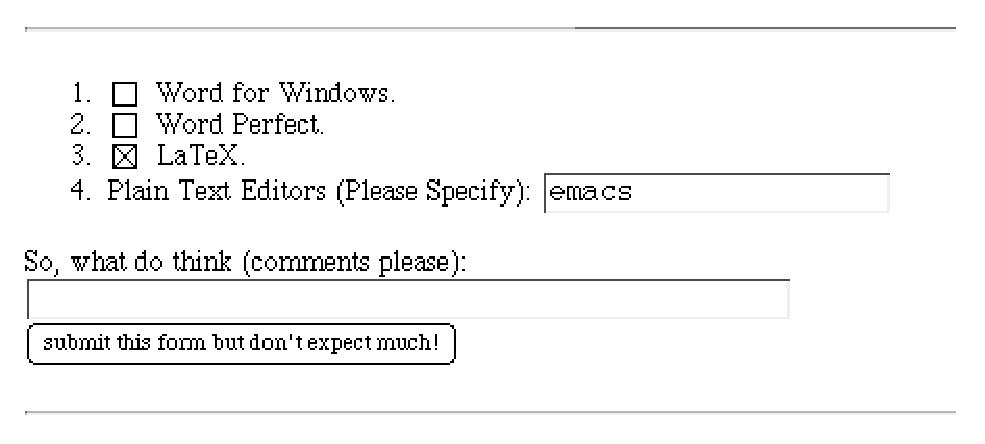
\includegraphics{psfiles/eform.ps}}}
    \end{center}
  \caption{An electronic form.
  In the online version the form would be active.}
  \label{eform}
\end{figure}
\end{latexonly}



\index{rawhtml@\Lc{rawhtml}}%
\paragraph*{\Lc{rawhtml}...\Lc{endrawhtml}\label{endrawhtml}}
\cbversion{97.1}\begin{changebar}
This is an alternative way to specify a chunk of raw \texttt{HTML} code,
using the old \AmS-style of delimiting environments.
Use of this style is discouraged; 
the \env{rawhtml} \htmlref{environment}{rawhtml} is preferred.%
\end{changebar}%

\index{comment@\env{comment} environment}%
\index{environment!comment@\env{comment}}%
\paragraph*{\Lc{begin\char123comment\char125}\label{comment}}
\cbversion{97.1}\begin{changebar}
This environment is simple for the convenience of ``commenting-out''
large sections of source code.
The contents of this environment is completely ignored,
both in the \LaTeX{} and \texttt{HTML} versions.
Such an environment is already used in \AmS-\LaTeX,
and perhaps with other packages.
It is defined here for its general utility.

\noindent
To insert \texttt{SGML}-style comments into the \texttt{HTML} files,
use the \env{rawhtml} environment as follows.
%begin{latexonly}
\begin{small}
%end{latexonly}
\begin{verbatim}
\begin{rawhtml}
<!--  this text is treated as a comment
      perhaps extending over several lines 
-->
\end{rawhtml}
\end{verbatim}
%begin{latexonly}
\end{small}
%end{latexonly}%
\end{changebar}%

\noindent
Note the \hyperref[page]{warning}{warning on page~}{}{env:warn}
concerning how the environment delimiters should be used in the
\LaTeX{} source code.


\index{latexonly@\Lc{latexonly}}%
\paragraph*{\Lc{comment...\char92endcomment}\label{endcomment}}
\cbversion{97.1}\begin{changebar}
This is an alternative way to specify a chunk of material intended
to be ignored in both the \LaTeX{} and \texttt{HTML} versions,
using the old \AmS-style of delimiting environments.
Use of this style (though convenient for typing) is discouraged,
since it is not as reliable as using the \env{comment} \htmlref{environment}{comment}.
\end{changebar}\html{\\}


\subsection{Arbitrary Tags and Attributes\label{sec:arbtags}}%
%\section{Arbitrary Tags and Attributes\label{sec:arbtags}}%
%
For version 97.1 of \latextohtml\ there is a new command which provides 
an extremely flexible way to include \texttt{HTML} 3.2 tags, along with
any values for the ``attributes'' of that tag, if desired.
\begin{quote}
\Lc{HTML}\verb|[|\Meta{attribs}\verb|]{|\Meta{tag}\verb|}|\label{HTMLtag}\\
\Lc{HTML}\verb|[|\Meta{attribs}\verb|]{|\Meta{tag}\verb|}{|\Meta{contents}\verb|}|
\end{quote}
When the \Meta{tag} also needs a closing tag (e.g \texttt{<I>...</I>})
the \Meta{contents} \emph{must} be given, enclosed in braces.
Both the opening and closing tags then will be placed correctly.


An important aspect of this is that any of the \Meta{tag},
\Meta{attribs} and \Meta{contents} may be given wholly
by expanding a \LaTeX{} macro, or may contain arbitrary macros, 
perhaps including other \Lc{HTML} commands.
\hyperref{The following table}{The contents of Figure~}{}{ex:HTML} 
was constructed using this feature; its \LaTeX{} source follows.

\HTML[50\% 3 noshade center]{HR}

\begin{htmlonly}
\begin{figure}
\begin{makeimage}
\end{makeimage}
\newcommand{\myalign}{center}
\newcommand{\mylist}{UL}
\newcommand{\myitem}[2]{\HTML[disc]{LI}{\simpletest{#1}{#2}}}
\newcommand{\simpletest}[2]{%
 \HTML{#1}{ a simple test of ``#2'',} using \HTML{CODE}{<#1>} .}
\newcommand{\tableopts}{10,border=5}

\newcommand{\tablelist}[4][\myalign]{\HTML[#1]{DIV}{
\HTML[\tableopts]{TABLE}{
\HTML[bottom]{CAPTION}{
#3
}\HTML{TR}{\HTML{TD}{
\HTML{#2}{
#4
}}}
}}\HTML[all]{BR}}

\tablelist[\myalign]{\mylist}{%
\textbf{A listing of the different text styles available in HTML 3.2}}{%
\myitem{B}{bold-face}
\myitem{I}{italics}
\myitem{TT}{teletype-text}
\myitem{U}{underlining}
\HTML[circle]{LI}{\simpletest{STRIKE}{strikeout}}
\myitem{EM}{emphasis style}
\myitem{STRONG}{strong style}
\myitem{CODE}{code style}
\myitem{CITE}{citation style}
\myitem{DFN}{definition style}
\HTML[square]{LI}{\simpletest{SAMP}{sample style}}
\HTML[square]{LI}{\simpletest{KBD}{keyboard style}}
\myitem{VAR}{variable style}}
%
 \caption{Example use of macros for raw \texttt{HTML} code.}
 \label{ex:HTML}
\end{figure}
\end{htmlonly}
%
\begin{latexonly}
\begin{figure}[ht]
\begin{center}
  \fbox{\scalebox{.7}{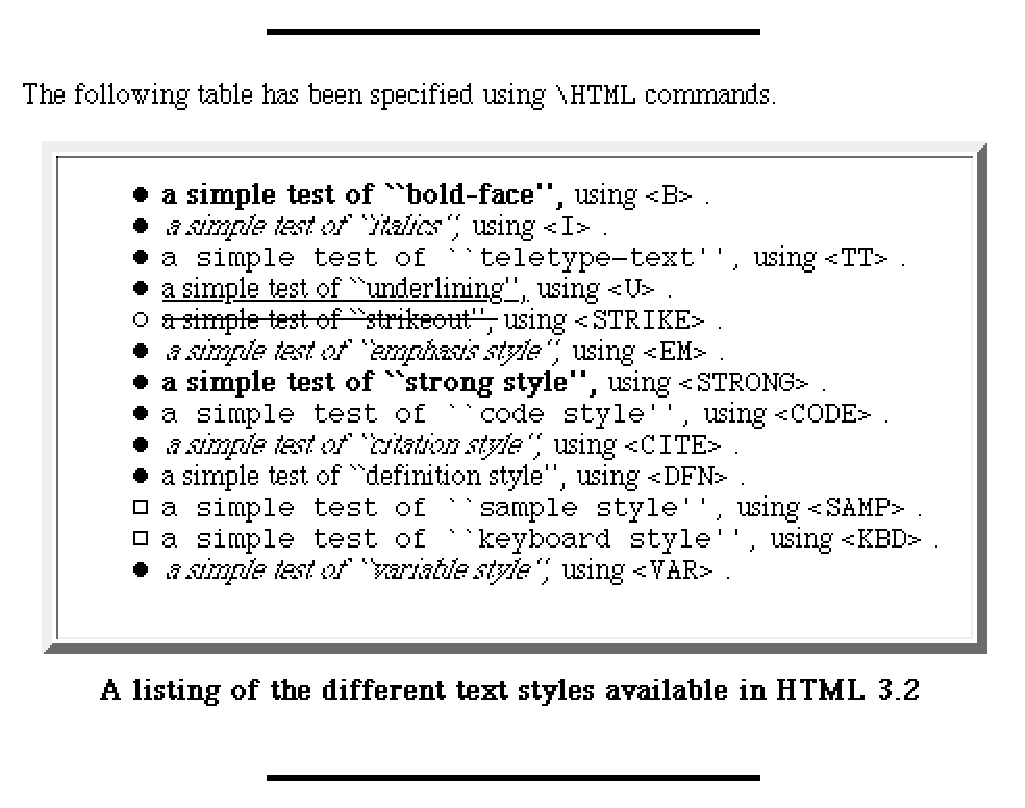
\includegraphics{psfiles/HTMLtab.ps}}}
 \caption{Example use of macros for raw \texttt{HTML} code.}
 \label{ex:HTML}
\end{center}
\end{figure}
\end{latexonly}

\HTML[50\% 3 noshade center]{HR}

%begin{latexonly}
\begin{small}
%end{latexonly}
\begin{verbatim}
\newcommand{\myalign}{center}
\newcommand{\mylist}{UL}
\newcommand{\myitem}[2]{\HTML[disc]{LI}{\simpletest{#1}{#2}}}
\newcommand{\simpletest}[2]{%
 \HTML{#1}{ a simple test of ``#2'',} using \HTML{CODE}{<#1>} .}
\newcommand{\tableopts}{10,border=5}

\newcommand{\tablelist}[4][left]{\HTML[#1]{DIV}{
\HTML[\tableopts]{TABLE}{
\HTML[bottom]{CAPTION}{
#3
}\HTML{TR}{\HTML{TD}{
\HTML{#2}{
#4
}}}
}}\HTML[all]{BR}}

\tablelist[\myalign]{\mylist}{%
\textbf{A listing of the different text styles available in HTML 3.2}}{%
\myitem{B}{bold-face}
\myitem{I}{italics}
\myitem{TT}{teletype-text}
\myitem{U}{underlining}
\HTML[circle]{LI}{\simpletest{STRIKE}{strikeout}}
\myitem{EM}{emphasis style}
\myitem{STRONG}{strong style}
\myitem{CODE}{code style}
\myitem{CITE}{citation style}
\myitem{DFN}{definition style}
\HTML[square]{LI}{\simpletest{SAMP}{sample style}}
\HTML[square]{LI}{\simpletest{KBD}{keyboard style}}
\myitem{VAR}{variable style}}
\end{verbatim}
%begin{latexonly}
\end{small}
%end{latexonly}

\HTML[50\% 3 noshade center]{HR}

\noindent
The above code demonstrates many aspects of the way \Lc{HTML}
commands can be used.
%
\begin{htmllist}\htmlitemmark{GreenBall}
\item [nesting: ] 
\Lc{HTML} commands can be nested to arbitrary depth.
%
\item [macros: ] 
Macros can be used to specify all or part of each argument.
%
\item [within macros: ] 
\Lc{HTML} commands work correctly within the expansions of other macros.
%
\item [attribute values: ]
Information within \Meta{attribs} can be specified in a very
loose way, as a comma-separated list of key/value pairs
or as single values. \\
Not even the commas are necessary: space(s), \Meta{tab}s 
or newlines are equally effective.
Indeed the horizontal rules preceding and following the table were 
specified by:
\begin{quote}
\begin{verbatim}
\HTML[50\% 3 noshade center]{HR}
\end{verbatim}
\end{quote}
%
\item [attribute names: ]
Usually it is \emph{not necessary} to know the names of the
attributes to the tags that are to be used. It is sufficient
just to give the values; these will be matched to the
appropriate attribute, according to the type of data required.
(If names are given, these are case-insensitive.)
%
\item [newlines: ] 
Although \LaTeX{} ignores linebreaks within the source code,
this is not so with \latextohtml. 
The strange spreading-out of the definition of the
\Lc{tablelist} command above was done with the purpose
solely of making the code in the resulting \texttt{HTML} files 
more easily readable, to a human.
(As most browsers ignore those newlines anyway, 
more compact code would have rendered the same on-screen.)
\end{htmllist}

\medskip\noindent
Some further aspects of the use of this \Lc{HTML}
command are not apparent from the above example. 

\begin{htmllist}\htmlitemmark{RedBall}
%
\item [invalid \Meta{tag}\,: ]
If a \Meta{tag} is specified that is not part of the 
\texttt{HTML} 3.2 specifications, then it and its attributes are 
not placed into the \texttt{HTML} document created by \latextohtml.
Any \Meta{contents} \emph{is} included as ordinary data; 
i.e. as text in paragraphs, etc.

\item [required attributes: ] 
Some tags have attributes which are required to have values,
if that tag is to be included in an \texttt{HTML} document.
Using the \Lc{HTML} command, if any such attribute
is not given an appropriate value then the tag is ignored.
Any \Meta{contents} are included in the document, 
as ordinary character data.

\item [valid HTML\,: ] 
Currently there is \emph{no} checking that the \Meta{contents}
of a \Meta{tag} contains only data (perhaps including other tags)
allowed by the DTD for \texttt{HTML} 3.2.
\begin{quote}
\textit{The requirement to produce valid \texttt{\upshape HTML} 
currently rests with the user.}
\end{quote}
This issue will be addressed in forthcoming revisions of \latextohtml.

\item [extra attributes and values: ]
The list of attributes for a \Meta{tag} can include
key-value pairs whose keys do not match any valid
attribute for the \Meta{tag}.
Such key-value pairs are simply ignored.
Similarly extra data values are ignored, 
as are values that do not match the
requirements for any valid attribute.

\item [attributes with similar data-types: ]
Several attributes to a \Meta{tag} may use values having 
the same or similar data-types. First any key-value pairs
are processed. Remaining values are allocated 
to those attributes which do not already have a value.
An ordering of the attributes is used, based on a perceived likelihood 
of each attribute being required to be changed from its default setting.

\end{htmllist}


\subsection{Conditional Text\label{sec:latexonly}}%
%\section{Conditional Text\label{sec:latexonly}}%
\tableofchildlinks*
\index{latexonly@\env{latexonly} environment}%
\index{htmlonly@\env{htmlonly} environment}%
\index{environment!htmlonly@\env{htmlonly}}%
\index{environment!latexonly@\env{latexonly}}%
\index{conditional text!scoped variant}\html{\\}%
\paragraph*{\Lc{begin\char123latexonly\char125} and 
\Lc{begin\char123htmlonly\char125}\label{latexonly}\label{htmlonly}}
Conditional text can be specified
using the environments \env{latexonly} and \env{htmlonly}. 
These allow writing parts of a document which are intended 
only for electronic delivery or only for paper-based delivery.

This would be useful for example in adding a long description of a
multi-media resource in the paper version of a document. 
Such a description would be redundant in the electronic version, 
as the user can have direct access to this resource. 

\medskip\goodbreak\noindent
Here is an example of the use of the \env{latexonly} environment,
used \hyperref[page]{earlier in}{on page~}{ of}{eform} this manual:
%begin{latexonly}
\begin{small}\indent
%end{latexonly}
\Lc{begin}\verb|{latexonly}|
\latex{\vskip-\baselineskip\vskip-\baselineskip}
\begin{verbatim}
\begin{figure}
    \begin{center}
    \fbox{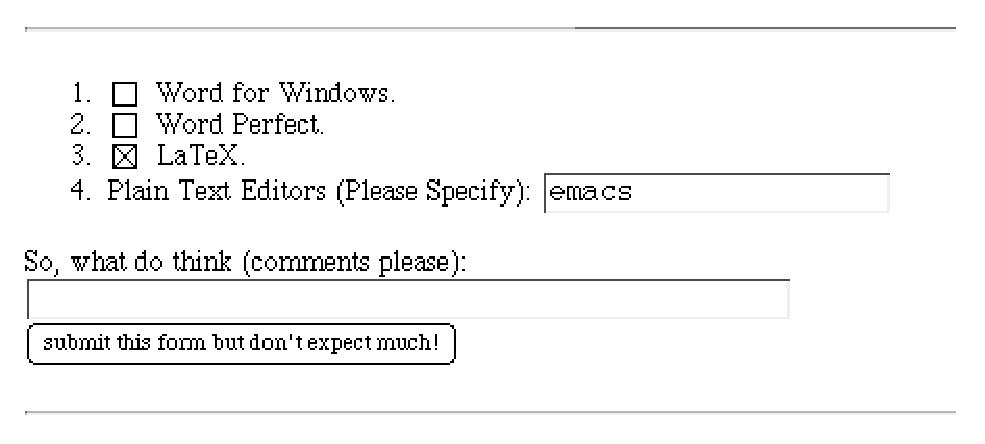
\includegraphics[width=4in]{psfiles/eform.ps}}
    \end{center}
    \caption{An electronic form. Of course in the online version of this
     document the form above would be active.}
\end{figure}
\end{verbatim}
\latex{\nobreak\vskip-\baselineskip\nobreak\indent\indent}%
\Lc{end}\verb|{latexonly}|
%begin{latexonly}
\end{small}\goodbreak\medskip
%end{latexonly}

\noindent
Note the \hyperref[page]{warning}{warning at the bottom of page~}{}{env:warn}
concerning how the environment delimiters should be used in the
\LaTeX{} source code.


\index{htmlonly@\Lc{htmlonly}}%
\paragraph*{\Lc{htmlonly...\char92endhtmlonly}\label{endhtmlonly}}
\cbversion{97.1}\begin{changebar}
This is an alternative way to specify a chunk of material intended
for the \texttt{HTML} version only,
using the old \AmS-style of delimiting environments.
Use of this style is discouraged; 
the \env{htmlonly} \htmlref{environment}{htmlonly} is preferred.%
\end{changebar}%


\index{latexonly@\Lc{latexonly}}%
\paragraph*{\Lc{latexonly...\char92endlatexonly}\label{endlatexonly}}
\cbversion{97.1}\begin{changebar}
This is an alternative way to specify a chunk of material intended
for the \LaTeX{} typeset version only,
using the old \AmS-style of delimiting environments.
Use of this style is discouraged; 
the \env{latexonly} \htmlref{environment}{latexonly} or the unscoped 
\htmlref{\texttt{\%begin\char123latexonly\char125}}{unlatexonly} 
construction are preferred.%
\end{changebar}%

\smallskip\noindent
Note the \hyperref[page]{warning}{warning at the bottom of page~}{}{env:warn}
concerning how the environment delimiters should be used in the
\LaTeX{} source code.


\index{conditional text!shorthand notation}%
\index{latex@\Lc{latex}}%
\index{html@\Lc{html}}%
\index{latexhtml@\Lc{latexhtml}}\html{\\}%
\paragraph*{\Lc{latex}, \Lc{html} and \Lc{latexhtml}\label{latexhtml}}
\cbversion{96.1}\begin{changebar}
There are also shorthand notations to accomplish the same thing 
as in the \env{latexonly} \htmlref{environment}{latexonly} and \env{htmlonly} 
\htmlref{environment}{htmlonly}, but with less typing.
\begin{itemize}
\item 
The \Lc{latex}\verb|{...}| command causes everything within the braces 
to be processed by \LaTeX, but ignored by \latextohtml.
\item  
Conversely, the \Lc{html}\verb|{...}| command causes everything within the braces 
to be ignored by \LaTeX{} and processed by \latextohtml.  
\item  
Finally the command \Lc{latexhtml}\verb|{...}{...}| causes everything 
within the first set of braces to be processed exclusively by \LaTeX, 
with the contents of the second set of braces processed solely by \latextohtml.%
\end{itemize}
\textbf{Warning: }
Only small pieces of text work reliably in this way. 
With whole paragraphs or contained sub-environments,
the ``conditional'' environments should be used instead.
\end{changebar}

\index{conditional text!without scope}%
\index{beginlatex@\texttt{\%{}begin\char123latexonly\char125}}%
\index{endlatex@\texttt{\%{}end\char123latexonly\char125}}%
\paragraph*{\texttt{\%begin\char123latexonly\char125}\label{unlatexonly}}
Another variant of the \env{latexonly} environment is available, 
in which everything between 
\verb|%|\verb|begin{latexonly}| and \verb|%|\verb|end{latexonly}| 
is ignored by \latextohtml.  
The difference is that the \env{latexonly} environment 
puts the contents into a group, in which all definitions are local.
There is no such scoping with the \verb|%begin...%end| variant,
since \LaTeX{} sees the initial \texttt{\%}s simply as starting comments.%

\medskip
\index{conditional text!example}\html{\\}\noindent
The following example should clarify what happens:
%begin{latexonly}
\begin{small}
%end{latexonly}
\begin{verbatim}
\newcommand{\A}{The letter A.}
\newcommand{\B}{The letter B.}
\end{verbatim}
\indent\indent\indent\verb|\|\verb|begin{latexonly}|\\
\indent\indent\verb|\renewcommand{\A}{Not the letter A.}|\\
\indent\indent\verb|\|\verb|end{latexonly}|\\
\indent\indent\verb|%|\verb|begin{latexonly}|\\
\indent\indent\verb|\renewcommand{\B}{Not the letter B.}|\\
\indent\indent\verb|%|\verb|end{latexonly}|
\begin{verbatim}
\begin{document}
\A \B
\end{document}
\end{verbatim}
%begin{latexonly}
\end{small}
%end{latexonly}
If you process this with \LaTeX, the result is: 
\quad\quad The letter A. Not the letter B.

\smallskip\noindent
Note the \hyperref[page]{warning}{warning at the bottom of page~}{}{env:warn}
concerning how the environment delimiters should be used in the
\LaTeX{} source code.

\medskip\index{conditional text!avoid using counters}\html{\\}\noindent
\textbf{Warning: }% 
Be careful when using \LaTeX{}  commands which alter the values of counters 
(e.g. numbered figures or equations) in conditional text, because this may 
cause the counter values in the electronic version to lose synchronisation 
with the values of the corresponding counters in the \LaTeX{} version.


\htmlrule[width=300]
\index{imagesonly@\env{imagesonly} environment}%
\index{environment!imagesonly@\env{imagesonly}}%
\paragraph*{\Lc{begin\char123imagesonly\char125}\label{imagesonly}}
\cbversion{97.1}\begin{changebar}
This environment is used to put \LaTeX{} code into the \fn{images.tex} file,
to be used when generating images. Typically this is used to add commands to
the preamble of \fn{images.tex}, such as setting the text or background color.
However code can be added at any other point as well; 
e.g. to change the background color of all images after a certain point in the document. 
\end{changebar}%

\smallskip\noindent
Note the \hyperref[page]{warning}{warning at the bottom of page~}{}{env:warn}
concerning how the environment delimiters should be used in the
\LaTeX{} source code.


\index{makeimage@\env{makeimage} environment}%
\index{environment!makeimage@\env{makeimage}}%
\paragraph*{\Lc{begin\char123makeimage\char125}\label{makeimage}}
\cbversion{97.1}\begin{changebar}
This is a special environment which forces an image to be made of its contents.
That is, one gets effectively a snapshot of a portion of a page
that has been typeset using \LaTeX. 
Within the normal \LaTeX{} typeset version of the document, this environment 
is completely transparent, adding its contents to the page as usual.

\index{makeimage@\env{makeimage} environment!inside@inside a \env{figure}}\html{\\}%
One further important use of the \env{makeimage} environment is as follows.
If a \env{makeimage} environment occurs as a sub-environment within 
a \env{figure} environment, then an image will \emph{not} be made of the
\env{figure}'s contents. Instead, the contents are treated as normal text,
each part being handled as if there were no \env{figure} at all,
except that everything is placed within a single cell of a
\HTMLtag{TABLE}...\HTMLtag{/TABLE} construction in \HTMLiii. 
The contents of any \Lc{caption}
commands are placed between \HTMLtag{CAPTION}...\HTMLtag{/CAPTION} tags 
for the \HTMLtag{TABLE}.

\index{makeimage@\env{makeimage} environment!empty sub-environment}\html{\\}%
Normally an image of the entire contents of the \env{figure} would be
placed within the single cell of the \HTMLtag{TABLE}.
Now images are made of any subparts of those \env{figure}'s contents 
that really need it, in particular the \env{makeimage} sub-environments.
An empty \env{makeimage} sub-environment does not generate an image of itself,
yet still it inhibits an image being made of the whole \env{figure}.
These comments apply also to \env{table} environments.
\end{changebar}\html{\\}




\subsection{Symbolic References shown as Hyperized Text\label{hyperized}%
%\section{Symbolic References shown as Hyperized Text\label{hyperized}%
\index{references@references\protect\label{IIIrefs}}}%
\tableofchildlinks*
\index{cross-references!|see{\htmlref{references}{IIIrefs}}}%
\index{references!symbolic\label{IIIsymref}}\index{symbolic labels|(}%
\index{references!numeric}%
\index{references!iconic}\html{\\}\noindent
In printed documents cross-references are shown 
through a \emph{numeric or symbolic indirection} 
e.g. ``see Figure 1'' (numeric indirection), 
or ``see section `Changes'~'' (symbolic indirection).  
\latextohtml{} can mirror this mechanism using the same numeric 
or symbolic references,
or when these are not appropriate by using iconic references.

\index{references!without indirection}%
\index{references!highlighted text}\html{\\}%
In a hypertext document however, cross-references can be shown 
without any indirection, just by highlighting a relevant piece of text. 
This can make a document more readable as it removes unnecessary
information. 

\index{hyperref@\Lc{hyperref}}%
\paragraph*{\Lc{hyperref}\label{hyperref}}
A single new \LaTeX{} command \Lc{hyperref} can be used for
specifying how a cross-reference should appear, 
both in the printed document and in the hypertext version.
For example, assuming that the label \verb|{sec:cond}|\label{sec:cond} 
is defined somewhere within a document, 
the command \Lc{hyperref}, taking 4 arguments,
can be used in that document as follows:
\index{hyperref@\Lc{hyperref}}%
\index{conditional text}%
%begin{latexonly}
\begin{small}
%end{latexonly}
\begin{verbatim}
\emph{Is the concept of
\hyperref
               % This will be highlighted in the hypertext version
{conditional text}			% argument #1
               % This will be shown in the printed version 
               % followed by a numeric reference ...      
{conditional text (see Section }  	% argument #2
               % ... followed by this text
{ for more information)} 		% argument #3
               % This is the common label 
{sec:cond}				% argument #4
a good idea? }
\end{verbatim}
%begin{latexonly}
\end{small}
%end{latexonly}

\noindent
Here is how it will be shown:
\begin{quote}
\emph{Is the concept of
\hyperref
% This will be highlighted in the hypertext version
{conditional text}
% This will be shown in the printed version  
% followed by a numeric reference ...      
{conditional text (see Section }  
% ... followed by this text
{ for more information)} 
% This the common label 
{sec:cond}
a good idea? }
\end{quote}

\begin{htmlonly}
In the printed version what would appear is:
\begin{quote}
\emph{Is the concept of conditional text (see Section 4.2 for more information) 
a good idea?}
\end{quote}
\end{htmlonly}

\begin{latexonly}%
In the hypertext version what would appear is:
\begin{quote}
\emph{Is the concept of \underline{conditional text} a good idea?}
\end{quote}
(Of course \underline{conditional text} would be an active hypertext link.)
\end{latexonly}

\bigskip\htmlrule[50\% center]
\cbversion{97.1}\begin{changebar}%
\noindent
An extended syntax for \Lc{hyperref} uses an optional argument, 
which determines what information is to be placed in the \LaTeX{} version
of the document. The value of this optional argument can also affect 
the number of required arguments. 
These forms are recognised:

%begin{latexonly}
\begin{small}
%end{latexonly}
\begin{quote}\label{hypernoref}
\Lc{hyperref}\verb|[ref]{|\Meta{HTML-text}\verb|}{|\Meta{LaTeX-text}%
\verb|}{|\Meta{post-LaTeX}\verb|}{|\Meta{label}\verb|}|\\
\Lc{hyperref}\verb|{|\Meta{HTML-text}\verb|}{|\Meta{LaTeX-text}%
\verb|}{|\Meta{post-LaTeX}\verb|}{|\Meta{label}\verb|}|\medskip

\Lc{hyperref}\verb|[pageref]{|\Meta{HTML-text}\verb|}{|\Meta{LaTeX-text}%
\verb|}{|\Meta{post-LaTeX}\verb|}{|\Meta{label}\verb|}|\\
\Lc{hyperref}\verb|[page]{|\Meta{HTML-text}\verb|}{|\Meta{LaTeX-text}%
\verb|}{|\Meta{post-LaTeX}\verb|}{|\Meta{label}\verb|}|\medskip

\Lc{hyperref}\verb|[noref]{|\Meta{HTML-text}\verb|}{|\Meta{LaTeX-text}%
\verb|}{|\Meta{label}\verb|}|\\
\Lc{hyperref}\verb|[no]{|\Meta{HTML-text}\verb|}{|\Meta{LaTeX-text}%
\verb|}{|\Meta{label}\verb|}|
\end{quote}
%begin{latexonly}
\end{small}
%end{latexonly}

\noindent
The first two are the defaults, where \LaTeX{} 
uses \Lc{ref}\verb|{|\Meta{label}\verb|}|.
With the next two \LaTeX{} uses \Lc{pageref}\verb|{|\Meta{label}\verb|}|,
while with the final two \LaTeX{} completely ignores the \Meta{label},
setting just the \Meta{LaTeX-text}.
\end{changebar}

\medskip
\index{hyperref@\Lc{hyperref}!pageref@\Lc{pageref} example}%
\html{\\}\noindent
For creating hyperlinks to other documents
using symbolic reference \Meta{label}s, 
see also the \Lc{externalref} 
\hyperref[page]{command}{command, described on page~}{}{externref}.

\medskip\noindent
The preceding paragraph is an example of the use of the \Lc{hyperref[page]} option.
Its source code is:
%begin{latexonly}
\begin{small}
%end{latexonly}
\begin{verbatim}
For creating hyperlinks to other documents
using symbolic reference \Meta{label}s, 
see also the \Lc{externalref} 
\hyperref[page]{command}{command, described on page~}{}{externref}.
\end{verbatim}
%begin{latexonly}
\end{small}
%end{latexonly}
\begin{htmlonly}
which appears in the \LaTeX{} typeset version as:
\begin{quote}
For creating hyperlinks to other documents
using symbolic reference \Meta{label}s, see also the
\Lc{externalref} command, described on page~31.
\end{quote}
\end{htmlonly}
\begin{latexonly}
which appears in the \texttt{HTML} version as:
\begin{quote}
For creating hyperlinks to other documents, using symbolic reference \Meta{label}s, 
see also the \Lc{externalref} \underline{command}.
\end{quote}
with the \underline{command} being an active hyperlink.
\end{latexonly}
\smallskip\noindent
In fact both \Lc{hyperref} and the \Lc{htmlref} command, to be described next,
permit textual hyperlinks based on symbolic \Meta{label}s from external files.


\index{htmlref@\Lc{htmlref}}%
\index{html.sty@\texttt{html.sty} style-file}
\paragraph*{\Lc{htmlref}\label{htmlref}}
Another command also defined in \fn{html.sty} is \Lc{htmlref} 
which has the same effect as \Lc{hyperref}
during the conversion to \texttt{HTML}.
It takes two arguments, some text and a label. 
In the \texttt{HTML} version the
text will be ``hyperized'', pointing to the label. 
In the paper version the text will be shown as it is 
and the label will be ignored; e.g.
%
\index{htmlref@\Lc{htmlref}!easy to make links}%
%begin{latexonly}
\begin{small}
%end{latexonly}
\begin{verbatim}
With \verb|\htmlref| \htmlref{it's easy to make links}{fig:example}.
\end{verbatim}
%begin{latexonly}
\end{small}
%end{latexonly}
which produces:
\begin{quote}
With \Lc{htmlref} \htmlref{it's easy to make links}{fig:example}.
\end{quote}
\begin{htmlonly}
In the \LaTeX{} typeset version it will appear simply as:
\begin{quote}
With \Lc{htmlref} it's easy to make links.
\end{quote}
\end{htmlonly}
\begin{latexonly}
In the \texttt{HTML} version it is shown as:
\begin{quote}
With \Lc{htmlref} \underline{it's easy to make links}.
\end{quote}
\end{latexonly}
\html{\\}
\goodbreak

\subsection{Hypertext Links in Bibliographic References (Citations)}%
%\section{Hypertext Links in Bibliographic References (Citations)}%
\tableofchildlinks*
\index{references!bibliographic}\index{bibliography|(}%
\index{bibliography!bibliographic database}%
\index{bibliography!using .bib@using \texttt{.bib} file}\html{\\}%
If a report or a book that is cited (using the \Lc{cite} command) 
is available (or there is information about it) on the World-Wide
Web, then it is possible to add the appropriate hypertext links
in your bibliographic database (the \texttt{.bib}) file. 

\bigskip
\index{bibliography!example using URLs}%
\index{bibliography!string commands@\texttt{\char64 string} commands}%
\index{LaTeX blue book@\LaTeX{} blue book}\html{\\}%
\noindent
Here is an example of a bibliographic entry for the original
\LaTeX{} \cite{lamp:latex} blue book:\nobreak
%begin{latexonly}
\begin{small}
%end{latexonly}
\begin{verbatim}
@string{curiaURL="\htmladdnormallink
{http://curia.ucc.ie/info/TeX/menu.html}
{http://curia.ucc.ie/info/TeX/menu.html}"}

@string{fernURL="\htmladdnormallink
{http://es-sun2.fernuni-hagen.de/info2html?(latex.info)Top}
{http://es-sun2.fernuni-hagen.de/info2html?(latex.info)Top}"}

@book{lamp:latex,
title = "LaTeX User's Guide \& Reference Manual, 2nd edition",
year = 1994 ,
author = "Leslie Lamport",
Publisher = "Addison--Wesley Publishing Company, Inc.",
note = "Online information on {\TeX} and {\LaTeX} is available at "
 # curiaURL # " and " # fernURL }
\end{verbatim}
%begin{latexonly}
\end{small}
%end{latexonly}
See the \htmlref{bibliography}{biblio} for how this will appear.\html{\\}
No other modifications are required; \LaTeX{} and Bib\TeX{} should work as normal.
%
\index{bibliography!string commands@\texttt{\char64string} commands}%
\cbversion{96.1f}\begin{changebar}
Note that it would be sensible to put the \texttt{@string} commands
into a separate file, \fn{urls.bib} say, 
loaded with the main file via\html{\\} \verb|\bibliography{urls,...}|.%
\end{changebar}

\smallskip\index{citations!Harvard style}%
\index{bibliography!Harvard style}\label{harvard}\html{\\}%
\noindent
For those who use the Harvard style for references
\htmladdnormallinkfoot{there exists a special conversion add-on package}%
{http://www.arch.su.edu.au/\~{}peterw/latex/harvard/}.

\index{citations!natbib@\env{natbib} package}%
\index{bibliography!natbib@\env{natbib} package}%
\index{citations!Harvard style!handled@handled by \env{natbib}}%
\cbversion{96.1g}\begin{changebar}
The \env{natbib} package, written for \LaTeX{} by \PatrickDaly,
provides even more flexibility in the way a reference may be cited. 
All the features of \htmlref{this package}{natbib} are implemented 
for \latextohtml{} via the \fn{natbib.perl} file.
(Indeed there is even a mode whereby \env{natbib} handles
the Harvard style of citation. 
This requires loading also the \env{nharvard} \htmlref{package}{nharvard}.)

\medskip
\noindent\textbf{Thanks...} to \Wilck\ for the bulk of the work 
in producing this extension, and to \RossMoore\ for 
necessary adjustments to allow it to work correctly with the 
\htmlref{document segmentation strategy}{Segmentation}.
\end{changebar}


\index{hypercite@\Lc{hypercite}}%
\paragraph*{\Lc{hypercite}\label{hypercite}}
\cbversion{97.1}\begin{changebar}
Analogous to \Lc{hyperref} is the \Lc{hypercite} command,
which allows a free-form textual hyperlink to the bibliography,
whereas the \LaTeX{} typeset version contains the usual citation code.
The allowed syntax is as follows.
%begin{latexonly}
\begin{small}
%end{latexonly}
\begin{quote}
\Lc{hypercite}\verb|[int]{|\Meta{HTML-text}\verb|}{|\Meta{LaTeX-text}%
\verb|}{|\Meta{opt-LaTeX}\verb|}{|\Meta{label}\verb|}|\\
\Lc{hypercite}\verb|[cite]{|\Meta{HTML-text}\verb|}{|\Meta{LaTeX-text}%
\verb|}{|\Meta{opt-LaTeX}\verb|}{|\Meta{label}\verb|}|\\
\Lc{hypercite}\Meta{HTML-text}\verb|}{|\Meta{LaTeX-text}%
\verb|}{|\Meta{opt-LaTeX}\verb|}{|\Meta{label}\verb|}|\medskip

\Lc{hypercite}\verb|[nocite]{|\Meta{HTML-text}\verb|}{|\Meta{LaTeX-text}%
\verb|}{|\Meta{label}\verb|}|\\
\Lc{hypercite}\verb|[no]{|\Meta{HTML-text}\verb|}{|\Meta{LaTeX-text}%
\verb|}{|\Meta{label}\verb|}|\\
\Lc{hypercite}\verb|[ext]{|\Meta{HTML-text}\verb|}{|\Meta{LaTeX-text}%
\verb|}{|\Meta{label}\verb|}|
\end{quote}
%begin{latexonly}
\end{small}
%end{latexonly}
The first three forms are equivalent; 
\LaTeX{} uses \Lc{cite}\verb|[|\Meta{opt-LaTeX}\verb|]|\Meta{label}\,,
after placing the \Meta{LaTeX-text}.
Note that \verb|{|\Meta{opt-LaTeX}\verb|}| \emph{must} be specified, 
even if empty `\verb|{}|'.

Similarly the latter three forms are equivalent, 
with \LaTeX{} using \Lc{nocite}\verb|{|\Meta{label}\verb|}|\,, 
to force the particular reference to appear on the bibliography page, 
even though no explicit marker is placed at this point.
(Thus there is no need for an optional  \Meta{opt-LaTeX} argument.)\html{\\}
Within the \texttt{HTML} version a hyperlink is produced when the \Meta{HTML-text} 
is not empty. External label files are also searched, 
in order to match the symbolic \Meta{label}, see also 
\hyperref[page]{\Lc{externalcite}}{\Lc{externalcite} on page~}{}{externcite}.

\smallskip\noindent\label{hyperciteXmpl}%
\index{hypercite@\Lc{hypercite}!example}%
\index{htmlcite@\Lc{htmlcite}!example}\html{\\}\noindent
\htmlref{Earlier}{hypcites} in this manual the following source code was used:
%begin{latexonly}
\begin{small}
%end{latexonly}
\begin{verbatim}
commands described in the \LaTeX{} \htmlcite{blue book}{lamp:latex}, 
...
as well as many other \LaTeX{} constructions, such as are described in 
the \LaTeX{} \hypercite{\emph{Companion}}{\emph{Companion}}{}{goossens:latex} 
and \LaTeX{} \hypercite{\emph{Graphics Companion} (e.g. \Xy-pic)}%
{\emph{Graphics Companion}}{\Xy-pic}{goossens:latexGraphics};
\end{verbatim}
%begin{latexonly}
\end{small}
%end{latexonly}
which produces:
\begin{quote}
commands described in the \LaTeX{} \htmlcite{blue book}{lamp:latex}, 
\\~~...\\
as well as many other \LaTeX{} constructions, such as are described in 
the \LaTeX{} \hypercite{\emph{Companion}}{\emph{Companion}}{}{goossens:latex} 
and \LaTeX{} \hypercite{\emph{Graphics Companion} (e.g. \Xy-pic)}%
{\emph{Graphics Companion}}{\Xy-pic}{goossens:latexGraphics};
\end{quote}
\begin{latexonly}
whereas in the \texttt{HTML} version one sees:
\begin{quote}
commands described in the \LaTeX{} \underline{blue book}, 
\\~~...\\
as well as many other \LaTeX{} constructions, 
such as are described in the \LaTeX{} \underline{\emph{Companion}} 
and  \LaTeX{} \underline{\emph{Graphics Companion} (e.g. \Xy-pic)};
\end{quote}
\end{latexonly}
%
\begin{htmlonly}
whereas in the \LaTeX{} typeset version one sees:
\begin{quote}
commands described in the \LaTeX{} blue book,\\
~~...\\
as well as many other \LaTeX{} constructions, such as are described in the \LaTeX{} 
\textit{Companion}[2] and \LaTeX{} \textit{Graphics Companion}[3, \Xy-pic];
\end{quote}
\end{htmlonly}
\end{changebar}%


\index{htmlcite@\Lc{htmlcite}}%
\paragraph*{\Lc{htmlcite}\label{htmlcite}}
\cbversion{97.1}\begin{changebar}
Analogous to \Lc{htmlref} is the \Lc{htmlcite} command,
which creates a textual hyperlink to a place on the document's bibliography page, 
but without displaying any reference marker in the \LaTeX{} typeset version.
(See \htmlref{above}{hyperciteXmpl} for an example.)%

The \Lc{externalcite} 
\hyperref[page]{command}{command, described on page~}{, }{externcite}
provides a similar facility when the bibliography page is ``external'';
that is, not part of the current document.%
\end{changebar}

\index{bibliography|)}



\subsection{Symbolic References between Living Documents\label{external_cross}}%
%\section{Symbolic References between Living Documents\label{external_cross}}%
\tableofchildlinks*
\index{external references|(}
\index{references!to external documents}%
\index{references!symbolic}%
\index{symbolic labels!see also@\emph{see also} 
 \htmlref{references, symbolic}{IIIsymref}}%
\index{labels!symbolic}%
%
\cbversion{96.1}\begin{changebar}
The method of the previous section to generated
symbolic \htmlref{hyperized}{hyperized} links can
easily be extended to \emph{external} documents processed by \latextohtml.  
When \latextohtml{} processes a document, it generates a \Perl{} file 
named \Meta{prefix}\fn{labels.pl}
which contains a list of all the symbolic labels that were defined, 
along with their locations.  
The \htmlref{\Meta{prefix}}{prefix} is empty unless otherwise specified, 
to allow different document segments to share the same directory.  
\end{changebar}

\index{externallabels@\Lc{externallabels}}%
\index{externalref@\Lc{externalref}}%
\paragraph*{\Lc{externallabels}\label{externlabels}}
\cbversion{96.1}\begin{changebar}
Links to an external document are then possible once a connection 
is established to that document's \fn{labels.pl} file.  
This connection is established by the \Lc{externallabels} command:%
\end{changebar}%
%
\begin{quote}
%begin{latexonly}
\begin{small}
%end{latexonly}
\Lc{externallabels}\verb|{|\Meta{URL to directory of external document}\verb|}|\\
\verb|               {|\Meta{local copy of external document labels.pl file}\verb|}|
%begin{latexonly}
\end{small}
%end{latexonly}
\end{quote}
%
\index{labels!external}\html{\\}%
The first argument to \Lc{externallabels} should be a URL to 
the directory containing the external document.  
The second argument
should be the full path-name to the \fn{labels.pl} file belonging
to the external document.  Note that for \emph{remote} external documents
it is necessary to copy the \fn{labels.pl} file locally so that it
can be read when processing a local document that uses it.
The command \Lc{externallabels} can be used once for each external
document in order to import the \textit{external labels}\label{externallabels}
into the current document.
A warning is given if \fn{labels.pl} cannot be found.

\begin{changebar}%
If a symbolic reference made in either of the commands described
\hyperref{on the previous page}{in Section~}{}{hyperized} is not 
defined within the document itself,
\latextohtml{} will look for that reference in one of the external
files\footnote{Care must be taken to ensure that critical symbolic
references are unique across related documents.}.
After any modifications in an external document 
(sections added/deleted, segmentation into different physical parts, etc.) 
a new \fn{labels.pl} will be generated.  
If the \Lc{externallabels} command in another 
document contains the correct address to an updated copy of
the \fn{labels.pl} file, then the cross-references will be re-aligned
after running the local document through the translator.

\index{labels!internal}\label{internallabels}\html{\\}%
There is also a mechanism analogous to the
\textit{label--ref} pairs of \LaTeX, which can be used only 
within a single document. 
These labels are called \textit{internal labels},
as opposed to the \htmlref{external labels}{externallabels} defined above.
They are used extensively with the document segmentation strategy
described \hyperref{later}{in Section~}{}{Segmentation}.

Either type of label is defined with a \LaTeX{} \Lc{label} command.  
Labels can be referenced \textit{within} a document using a \Lc{ref} command.
When processed by \LaTeX, each \Lc{ref} command is replaced by the 
section number in which the corresponding \Lc{label} occurred.
When processed by the translator, each \Lc{ref} is replaced by 
a hypertext link to the place where the corresponding \Lc{label} occurred.%
\end{changebar}%
 

\index{references!to external documents}%
\index{externalref@\Lc{externalref}}%
\paragraph*{\Lc{externalref}\label{externref}}
\begin{changebar}%
This mechanism can be extended to external documents:
\begin{quote}
%begin{latexonly}
\begin{small}
%end{latexonly}
\Lc{externalref}\verb|{|\Meta{symbolic label in remote document}\verb|}|
%begin{latexonly}
\end{small}
%end{latexonly}
\end{quote}
The argument to \Lc{externalref} may be any symbolic label defined 
in the \fn{labels.pl} file of any of the external documents.
Such references to external symbolic labels are then translated
into hyper-links pointing to the external document.%
\end{changebar}%


\index{citations!within external bibliographies}%
\index{externalcite@\Lc{externalcite}}%
\paragraph*{\Lc{externalcite}\label{externcite}}
\cbversion{97.1}\begin{changebar}
%
Analogous to \htmlref{\Lc{externalref}}{externref},
the \Lc{externalcite} command is used to create a citation link,
where the bibliography page is not part of the current document.
As with \Lc{externalref} symbolic labels for the bibliography page
must have been loaded using 
\htmlref{\Lc{externallabels}}{externlabels}.

A particularly important use for this is in allowing multiple documents 
to access information in a common bibliographic listing.
For example: all of an author's publications; 
a comprehensive listing of publications in a particular field; 
the (perhaps yearly) output of publications 
from a particular organisation or institution.

\medskip\noindent
\textbf{Thanks...} to \Engberg\ for suggesting this feature.
\end{changebar}

\index{external references|)}


\subsubsection{Cross-Referencing Example\label{crossrefs}}% 
%\subsection{Cross-Referencing Example\label{crossrefs}}% 
To understand this mechanism better consider 
how you would maintain a link to this section  
(of the hypertext version of this document) from one of your documents,
without using labels.
Sure enough you can get the name of the physical file that this section is in. 
This however is quite likely to change, and any links to it would become invalid. 
\index{link validation!done by hand}%
To update your link, the name of the new file must be found 
and your link changed by hand. 
Also there is no general updating mechanism, so the only way to find
out if your document is pointing to the right place is by actually
following the link, then doing a manual update\footnote{%
Link validation can be done automatically but the updating must be done
manually when filenames have changed (assuming no other symbolic label
mechanism is available).}.

\index{link validation!symbolic labels}\html{\\}%
Next consider how it could be done with symbolic labels. 
First you have to import the labels used in this document 
by copying the file \htmladdnormallink{\fn{labels.pl}}
{http://cbl.leeds.ac.uk/nikos/tex2html/doc/manual/labels.pl},
saving it in \path{/tmp/labels.pl} say,
then adding anywhere in your document:
%begin{latexonly}
\begin{small}
%end{latexonly}
\begin{verbatim}
\externallabels{http://cbl.leeds.ac.uk/nikos/tex2html/doc/manual}%
               {/tmp/labels.pl}
\end{verbatim}
%begin{latexonly}
\end{small}
%end{latexonly}
After that you can use the label `\texttt{crossrefs}' defined at the beginning of this 
section\footnote{You either have to guess the role of each label by
looking at the \fn{labels.pl} file or by asking the author!} as follows:
%begin{latexonly}
\begin{small}
%end{latexonly}
\begin{verbatim}
\externalref{crossrefs}
\end{verbatim}
%begin{latexonly}
\end{small}
%end{latexonly}
This will be translated into the appropriate hyper-link to this page.
If there are any changes in this document and you would like to
bring your document up-to date, you have to copy 
\htmladdnormallink{\fn{labels.pl}}%
{http://cbl.leeds.ac.uk/nikos/tex2html/doc/manual/labels.pl} again
and rerun the translator on your document. Of course if I move the 
directory containing the \texttt{HTML} files for this document somewhere else, 
then you would have to make a change in the argument of the 
\Lc{externallabels} command to reflect this. 

\index{references!collaboration required}%
It is obvious that some level of collaboration is required between
authors trying to maintain cross-references between different documents. 
Using symbolic labels makes this a lot easier 
(especially for documents written by the same author).
\index{symbolic labels|)}



\subsection{Miscellaneous commands for \texttt{HTML} effects\label{misceffects}}%
%\section{Miscellaneous commands for \texttt{HTML} effects\label{misceffects}}%
\tableofchildlinks*
\index{html.sty@\texttt{html.sty} style-file}%

\noindent
The \env{html} package, through the \LaTeX{} input file \fn{html.sty},
and its \Perl{} counterpart \fn{html.perl}, implements several 
new commands that are intended entirely for effects within the
produced \texttt{HTML} files. In \LaTeX{} these commands, their arguments,
and any optional arguments are completely ignored.

\index{htmlrule@\Lc{htmlrule}}%
\index{visual separation!using \Lc{htmlrule}}%
\paragraph*{\Lc{htmlrule } and 
 \Lc{htmlrule*}\label{htmlrule}}
One such device provided by \fn{html.sty},
is the \Lc{htmlrule} command. 
This puts a horizontal rule into the \texttt{HTML} file only;
being ignored in the \texttt{.dvi} version. 
It is useful to provide extra visual separation between paragraphs,
without creating a new \texttt{HTML} page, 
such as might warrant extra vertical space within the printed version.

\index{htmlrule!htmlrulestar@\Lc{htmlrule*}}%
\index{htmlrule!variants}%
\index{htmlrule!attributes@attributes to the \HTMLtag{HR} tag}%
\cbversion{97.1}\begin{changebar}
Much variation can be obtained in the horizontal rule that is produced,
using extended forms of the \Lc{htmlrule} command:
\begin{quote}
%begin{latexonly}
\begin{small}
%end{latexonly}
\Lc{htmlrule}\\
\Lc{htmlrule*}\\
\Lc{htmlrule[}\Meta{attribs}\texttt{]}\\
\Lc{htmlrule*[}\Meta{attribs}\texttt{]}
%begin{latexonly}
\end{small}
%end{latexonly}
\end{quote}
Whereas a ``break'' tag \HTMLtag{BR} normally precedes the \HTMLtag{HR} generated
by the \Lc{htmlrule} command, 
this break is omitted when using the \Lc{htmlrule*} variant. 

\htmlrule[center,width=200]

\noindent
Furthermore, the optional argument \Meta{attribs} can be used to specify 
attributes for \emph{both} the \HTMLtag{HR} and \HTMLtag{BR} tags. 
More specifically, \Meta{attribs} should be a list of attribute-names 
and/or key-value pairs \texttt{\Meta{key}=\Meta{value}} separated by spaces or commas. 
This list is parsed to extract those attributes applicable to the \HTMLtag{HR} tag,
and those applicable to the \HTMLtag{BR} (with the unstarred variant).

\medskip\htmlrule[right,width=200,size=5]
\noindent
Using \HTMLiii, this allows variations to be specified for:
\begin{itemize}
\item 
the (vertical) thickness of the horizontal line in pixels: \texttt{SIZE=\Meta{num}};
\item 
the (horizontal) width of the line in pixels or points: \texttt{WIDTH=\Meta{width}};
\item 
alignment: \texttt{WIDTH=\char34...\char34 } 
taking \texttt{left}, \texttt{right} or \texttt{center};
\item 
removal of the shadowed effect \texttt{NOSHADE};
\item 
positioning of the rule with respect to text-flows: 
\texttt{CLEAR=\char34...\char34 } 
taking \texttt{left}, \texttt{all}, \texttt{right} or \texttt{none}. 
\htmlrule[right,width=200,size=5]
\end{itemize}%
Some examples of these effects appear on 
\latex{the \texttt{HTML} version of} this page.%
\end{changebar}%


\index{strikeout@\Lc{strikeout}}%
\paragraph*{\Lc{strikeout\char123}\Meta{text}\texttt{\char125}\label{strikeout}}
\cbversion{97.1}\begin{changebar}
With this command the \Meta{text} is processed as normal in the \texttt{HTML} version,
then placed between \HTMLtag{STRIKE}...\HTMLtag{/STRIKE} tags.
Thus a horizontal line should be drawn through the middle of the \Meta{text}.\html{\\}
Currently the command and the \Meta{text} are ignored in the \LaTeX{} version.%
\end{changebar}%


\index{tableofchildlinks@\Lc{tableofchildlinks}}%
\paragraph*{\Lc{tableofchildlinks }\label{tochlinks}}
\cbversion{97.1}\begin{changebar}
As an extra aid to navigation within a long page, 
containing several (sub)subsections or deeper levels of sectioning,
there is the \Lc{tableofchildlinks} command.
This does not generate anything new, for a table of the child links
on or from a page is generated automatically by \latextohtml.

However if this command, or its variant \Lc{tableofchildlinks*},
occurs within the source code to appear on a particular \texttt{HTML} page,
then the child-links table will be placed at that point
where the command occurs. 
Normally a break tag \HTMLtag{BR} is inserted to separate the table of child-links 
from the surrounding text. The \Lc{tableofchildlinks*} omits this extra break
when it would result in too much space above the table.

For example throughout this section of the \latex{\texttt{HTML} version of the }manual, 
all subsections in which several explicit commands have been discussed
have their child-links table placed at the top of the page,
using \Lc{tableofchildlinks*}. 
This helps to quickly find the description of how the commands are used.%
\end{changebar}%


\index{htmlinfo@\Lc{htmlinfo}}%
\paragraph*{\Lc{htmlinfo }\label{htmlinfo}}
\cbversion{97.1}\begin{changebar}
Normally an ``About this document...'' page is created at the end
of the \texttt{HTML} document, containing technical information
about how the document was created, by whom, or any other information
contained in the \fn{\$INFO} \htmlref{variable}{infostring}.
This information can be made to appear at any other place within the document 
by specifying \Lc{htmlinfo} at the desired place in the source.
For example, the information may be best suited for the title-page.

The variant \Lc{htmlinfo*} places the information, but leaves out the 
standard ``About this document...'' header. 
Instead the \htmlref{\Lc{htmlhead}}{htmlhead} command 
can be used to place an alternative heading, prior to the \Lc{htmlinfo*} command.
Neither this heading nor the \fn{\$INFO} \htmlref{contents}{infostring} appears 
in the \LaTeX{} typeset version.%
\end{changebar}%


\index{bodytext@\Lc{bodytext}}%
\paragraph*{\Lc{bodytext\char123}\Meta{options}\texttt{\char125}\label{bodytext}}
\cbversion{96.1g}\begin{changebar}
The text and background colors, and colors for the text of hypertext links can
be set on an \texttt{HTML} page by giving appropriate attributes 
with the \HTMLtag{BODY ...} tag. This is particularly easy to do
using the \Lc{bodytext} command, 
which simply inserts the \Meta{code} as the desired list of attributes.%

\medskip
\index{bodytext@\Lc{bodytext}!no checking for valid attributes}\html{\\}%
\noindent
\textbf{Warning: }Any previous settings for the \HTMLtag{BODY ...} tag
are discarded. Furthermore no checking is done to verify whether the given \Meta{options}
indeed contains a list of attributes and values valid for the \HTMLtag{BODY ...} tag.\html{\\}
When using \Lc{bodytext} you are assumed to know precisely what you are doing!

\medskip\noindent
Other packages contain commands which alter the contents of the \HTMLtag{BODY ...} tag;
notably the \fn{color.perl} implementation of \LaTeX's \env{color} package,
and the (prototype) \env{frames} package, by \Wilck\ and \RossMoore.
In both these packages the requested information is checked for
validity as an attribute within the \HTMLtag{BODY ...} tag.
\end{changebar}%

\index{htmlbody@\Lc{htmlbody}}%
\paragraph*{\Lc{htmlbody\char123}\Meta{options}\texttt{\char125}\label{htmlbody}}
\cbversion{97.1}\begin{changebar}
This is similar to the \Lc{bodytext} command, except that it adds the
value of an attribute, or allows an existing value to be changed.
Thus it can be used to alter just a single one of the text and background colors, 
colors for the text of hypertext links or add a background pattern.
The \Meta{options} are given as key-value pairs; some checking is done to ensure 
the validity of the attributes whose values are being set.%
\end{changebar}%

\index{htmlbase@\Lc{htmlbase}}%
\paragraph*{\Lc{htmlbase\char123}\Meta{URL}\texttt{\char125}\label{htmlbase}}
\cbversion{96.1g}\begin{changebar}
This specifies that the given \Meta{URL} be included in the \HTMLtag{HEAD} section
of each \texttt{HTML} page via a tag: 
\texttt{<BASE HREF=\char34\Meta{URL}\char34}.\html{\\}
Such a feature is particularly useful\dots 
\begin{itemize}
\item
when preparing a document whose final location may be different from where it was created; 
By making all internal references be relative (to the the provided \Meta{URL}),
a whole directory tree containing the document 
and all its subparts can be moved to elsewhere.
A single edit in each \texttt{HTML} file produces the complete document intact 
at the new location.
%
\item
by allowing just single page to be copied to another location, but act as if it were
part of the original document (provided this is accessible across the Web).
Relative URLs within the copied page are relative to the base \Meta{URL},
rather than relative to the new location.
%
\item
Other uses for this feature are likely to become apparent.%
\end{itemize}\end{changebar}%


\index{HTMLset@\Lc{HTMLset}!alters a \Perl{} variable}%
\index{HTMLset@\Lc{HTMLsetenv}!alters a \Perl{} variable}%
\paragraph*{\Lc{HTMLset\char123}\Meta{which}\texttt{\char125\char123}%
\Meta{value}\texttt{\char125} and 
\Lc{HTMLsetenv\char123}\Meta{which}\texttt{\char125\char123}%
\Meta{value}\texttt{\char125}\label{HTMLset}}
\cbversion{97.1}\begin{changebar}
The \Lc{HTMLset} command provides a mechanism whereby an arbitrary
\Perl{} variable can be assigned a value dynamically, during the \latextohtml{} processing. 
A variable having name `\texttt{\$}\Meta{which}' is assigned the specified \Meta{value},
overwriting any value that may exist already. The \Lc{HTMLsetenv} is for the same purpose,
but it is expanded in order as if it were an environment, rather than a command.

\medskip\noindent
\textbf{Warning: }This is intended for \Perl{} programmers only.
Use this command at your own risk!
\end{changebar}

\htmlrule[width=300]
\index{LaTeX2HTML@\latextohtml{}!command for its name}%
\index{names of important packages}%
\index{latextohtml@\Lc{latextohtml}!gives @gives \latextohtml{}}%
\paragraph*{\Lc{latextohtml}\label{l2hname}} 
\cbversion{97.1}\begin{changebar}
expands to the name \latextohtml, of this translator.
Commands for parts of names of important \LaTeX{} packages are also 
included with \latextohtml: e.g. \TeX, \LaTeX, \AmS, \Xy\,.
(This is to make it easy to refer to these products, in a consistent way
within the \texttt{HTML} pages; you may still need \LaTeX{} definitions
for the typeset version.)
\end{changebar}
\medskip



\subsection{Active Image Maps\label{ImageMaps}}%
%\section{Active Image Maps\label{ImageMaps}}%
\index{images!image-maps|(}\index{image-map!map-file}%
\index{HTML@\texttt{HTML}!Version 3.2}%
\index{usemap@\texttt{usemap}}%
\index{thumbnail}%
\cbversion{96.1}\begin{changebar}%
\emph{Image maps} are images with active regions in which a 
Web-surfer can click, to send him off to another sector of cyberspace.  
\latextohtml{} can design either inline ``figures'' or external ones 
(with or without a thumbnail version) to be image-maps.  
However \texttt{HTML} requires a URL of a \texttt{HTML} \emph{map-file}, 
which associates the coordinates of each active region in
the map with a destination URL.  
Usually this map file is kept on the server machine, 
however \texttt{HTML} 3.2 also allows it 
to reside on the \htmladdnormallink{client side}%
{http://ds.internic.net/internet-drafts/draft-seidman-clientsideimagemap-02.txt} 
for faster response.  
Both configurations are supported by \latextohtml{} 
through the \Lc{htmlimage} options
`\texttt{map=}' and `\texttt{usemap=}' respectively.

\index{makemap@\texttt{makemap}}%
\index{image-map!user-map file}\html{\\}%

Keeping such a map file up to date manually can be tedious, 
especially with dynamic documents under revision.
An experimental program \fn{makemap} helps automate this process.  
This program (which is really a \Perl{} script)
takes one mandatory argument and an optional argument.
The mandatory argument is the name of a \emph{user-map} file,
defined below.  The optional argument is the name of the
directory where the \texttt{HTML} map file(s) are to be placed.

\index{image-map!example}\html{\\}%
The best way of describing how this works is by example.
Suppose a document has two figures designated to
become active image-maps.  The first
figure includes a statement like:
%begin{latexonly}
\begin{small}
%end{latexonly}
\begin{verbatim}
\begin{figure}
\htmlimage{map=/cgi-bin/imagemap/BlockDiagram.map,...}
. . .
\end{figure}
\end{verbatim}
%begin{latexonly}
\end{small}
%end{latexonly}
The second figure has a line like:

%begin{latexonly}
\begin{small}
%end{latexonly}
\begin{verbatim}
\begin{figure}
\htmlimage{map=/cgi-bin/imagemap/FlowChart.map,...}
. . .
\end{figure}
\end{verbatim}
%begin{latexonly}
\end{small}
%end{latexonly}

\medskip\htmlrule[50\% center]
\index{image-map!CERN server}\index{CERN!image-map server}%
\index{image-map!NCSA server}\index{NCSA!image-map server}%
\index{image-map!example}\html{\\}%
\noindent
A typical user-map file, named \fn{report.map}, 
might contain the following information\footnote{%
This file is designed for an \appl{NCSA} server.  
\appl{CERN} servers use ``\texttt{rect}''
instead of ``\texttt{rectangle},'' 
specify a radius instead of an outer point in the circle, 
and enclose point coordinates by parentheses.}:
%begin{latexonly}
\begin{small}
%end{latexonly}
\begin{verbatim}
#
#  Define the location(s) of the labels.pl file(s):
#
+report/ <URL>
#
#  Define map #1:
#
BlockDiagram.map:       
label1  rect    288,145 397,189
label2  rect	307,225 377,252
label2  default
#
#  Define map #2
#
FlowChart.map:
label3  circle  150,100 200,100
label4  default
\end{verbatim}
%begin{latexonly}
\end{small}
%end{latexonly}
\index{symbolic labels}\html{\\}%
In this file, comments are denoted by a \texttt{\#}-sign in column~1.
The line beginning with \verb|+report| states that the symbolic labels
are to be found in the \fn{labels.pl} contained in the directory
\path{report/ }, and that its associated URL is as stated.  Any number
of external \fn{labels.pl} files may be so specified.
The block diagram image has two active regions.  The first is a rectangle
bounded by corners (288, 145) and (397, 189), while the second is a rectangle
bounded by corners (307, 225) and (377, 252).  These coordinates
can be obtained with the aid of a program such as \fn{xv}.
If the user clicks in the first rectangle, 
it will cause a branch to the URL associated
with symbolic label \texttt{label1} defined in the \fn{labels.pl} file
found in directory \path{report/ }.  The single active region in the
flow chart figure is a circle centred at (150, 100) and passing through
point (200, 100).  Clicking in this region will cause a branch to
symbolic label \texttt{label3}.  Labels \texttt{label2} and \texttt{label4}
will be visited if the user clicks anywhere outside of the explicit
regions.  If any labels are not defined in any of the \fn{labels.pl}
files mentioned, they will be interpreted as URLs without translation.

The \texttt{HTML} image-maps are generated and placed in directory
\path{report/ } by invoking the command: \verb| makemap report.map report |.%
\end{changebar}\par
\index{images!image-maps|)}




\subsection{Document Segmentation\protect\footnote{This feature
%\section{Document Segmentation\protect\footnote{This feature
is supported only for users of \LaTeXe.}\label{Segmentation}}%
\tableofchildlinks*\htmlrule
\index{segmentation|(}%
\cbversion{96.1}\begin{changebar}
One of the greatest appeals of the World-Wide Web is its high
connectivity through hyper-links.  As we have seen, the \LaTeX{} 
author can provide these links either manually or symbolically.
Manual links are more tedious because a URL must be provided
by the author for every link, and updated every time the target
documents change.
\index{segmentation!symbolic links}%
Symbolic links are more convenient, 
because the translator keeps track of the URLs.  
Earlier releases of \latextohtml\ required the entire document 
to be processed together if it was to be linked symbolically.  
However it was easy for large documents to overwhelm 
the memory capacities of moderate-sized computers.  
Furthermore, processing time could become prohibitively high, 
if even a small change required the entire document to be reprocessed.

\index{document!segments}\index{segmentation!document segments}%
\index{segmentation!shared references}\html{\\}%
For these reasons, program segmentation was developed.
This feature enables the author to subdivide his document
into multiple \textit{segments}\label{segments}.
Each segment can be processed independently by \latextohtml.
Hypertext links between segments can be made symbolically,
with references shared through auxiliary files.  
If a single segment changes, only that segment needs to be reprocessed 
(unless a label is changed that another segment requires).  
Furthermore, the entire document can be processed 
without modification by \LaTeX{} to obtain the printed version.  

\index{segmentation!parent segment}%
\index{segmentation!child segments}\html{\\}\noindent
The top level segment that \LaTeX{} reads is called the \emph{parent} segment.
\html{\\}
The others are called \emph{child} segments.

\index{segmentation!requires book-keeping}\html{\\}\noindent
Document segmentation does require a little more work on the
part of the author, who will now have to undertake some
of the book-keeping formerly performed by \latextohtml.
The following four \LaTeX{} extensions carry out segmentation:

\begin{htmllist}\htmlitemmark{BlueBall}%
%
\index{segment@\Lc{segment}}%
\item [ \Lc{segment\char123}\Meta{file}\texttt{\char125\char123}\Meta{sec-type}%
 \texttt{\char125\char123}\Meta{heading}\texttt{\char125}\label{segment}]
%
This command indicates the start of a new program segment.
The segment resides in \Meta{file}\texttt{.tex}, represents the start
of a new \LaTeX{} sectional unit of type \Meta{sec-type}
(e.g., \Lc{section}, \Lc{chapter}, etc.) and has a heading
of \Meta{heading}.  (A variation \Lc{segment*} of this command, 
is provided for segments that are \emph{not} to appear in the table of contents.)\html{\\}  
These commands perform the following operations in \LaTeX:
%
\begin{enumerate}
\item 
The specified sectioning command is executed.
\item 
\LaTeX{} will write its section and equation counters
into an auxiliary file, named \Meta{file}\texttt{.ptr}.  It will also
write an \Lc{htmlhead} command to this file.  This
information will tell \latextohtml\ how to initialise itself
for the new document segment.
\item 
\LaTeX{} will then proceed to input and process the file \Meta{file}\texttt{.tex}.
\end{enumerate}
The \Lc{segment} and \Lc{segment*} commands are ignored by
\latextohtml.

\index{internal@\Lc{internal}}%
\item [ \Lc{internal[}\Meta{type}\texttt{]\char123}%
 \Meta{prefix}\texttt{\char125}\label{internal}]
%
This command directs \latextohtml\ to load inter-segment information 
of type \Meta{type} from the file \Meta{prefix}\Meta{type}\texttt{.pl}~.  
Each program segment must be associated with a unique \htmlref{filename-prefix}{prefix}, 
specified either through a command-line option, 
or through the installation variable \fn{\$AUTO\_PREFIX}~.
The information \Meta{type} must be one of the following:
%
\begin{htmllist}\htmlitemmark{OrangeBall}\addtolength{\leftskip}{15pt}%
%
\index{internals!labels from other segments}%
\index{segmentation!data about labels}%
\item[\texttt{internals}]  
This is the default type, which need not be
	given.  It specifies that the
	\htmlref{internal labels}{internallabels} from the
	designated segment are to be input and made available
	to the current segment.  
\html{\\}%
\index{contents!from other segments}%
\index{segmentation!data about contents}%
\item[\texttt{contents}]  
The table of contents information from
	designated segment are to be made available to the
	current segment.
\html{\\}%
\index{sections!from other segments}%
\index{segmentation!data about sections}%
\item[\texttt{sections}]  
Sectioning information is to be read in.
	Note that the segment containing the table of contents
	requires both contents and sections information
	from all other program segments.
\html{\\}%
\index{figures!from other segments}%
\index{list of figures}%
\index{segmentation!data about figures}%
\item[\texttt{figure}]  
Lists of figures from other segments are to be read.
\html{\\}%
\index{tables!from other segments}%
\index{list of tables}%
\index{segmentation!data about tables}%
\item[\texttt{table}] 
Lists of tables from other segments are to be read.
\html{\\}%
\index{index!data from other segments}%
\index{segmentation!data for the index}%
\item[\texttt{index}] 
Index information from other segments is to be read.
\html{\\}%
%\item[\texttt{indexkeys}] Index information from other segments are to be read.
%\item[\texttt{subindexkeys}] Index information from other segments are to be read.
\end{htmllist}
\cbversion{96.1f}\begin{changebar}
\index{index!short prefixes preferred}%
\index{index!cumbersome}\html{\\}%
\textbf{Note: } If extensive indexing is to be used, then it is advisable
to keep each \Meta{prefix} quite short. This is because the hyper-links
in the index have text strings constructed from this \Meta{prefix},
when using the \env{makeidx} package. Having long names with
multiply-indexed items results in an extremely inelegant, cumbersome index.
See \hyperref{the section on indexing}{Section~}{}{index} for more details.%
\end{changebar}


\index{startdocument@\Lc{startdocument}}%
\index{segmentation!starting a segment}%
\item [ \Lc{startdocument}\label{startdoc}]
%
The \Lc{begin}\verb|{document}| and  \Lc{end}\verb|{document}|
statements are contained in the parent segment only.  
It follows that the child segments cannot be processed
separately by \LaTeX{} without modification.  However they can be
processed separately by \latextohtml, provided it is told
where the end of the \LaTeX{} preamble is;  this is
the function of the \Lc{startdocument} directive.  It 
substitutes for \Lc{begin}\verb|{document}| in child segments, 
but is otherwise ignored by both \LaTeX{} and \latextohtml.

\index{htmlhead@\Lc{htmlhead}}%
\item [ \Lc{htmlhead\char123}\Meta{sec-type}%
 \texttt{\char125\char123}\Meta{heading}\texttt{\char125}\label{htmlhead}] 
%
This command is generated automatically by 
a \htmlref{\Lc{segment}}{segment} command. 
It is not normally placed in the document at all; instead it facilitates 
information being passed from parent to child 
via the \Meta{file}\texttt{.ptr} file.\html{\\}  
It identifies to \latextohtml\ that the current segment 
is a \LaTeX{} sectional unit of type \Meta{sec-type}, with the specified heading.\html{\\}
This command is ignored by \LaTeX. %
\cbversion{97.1}\begin{changebar}
From version \textsc{v97.1}\,, it is possible to use this command to insert extra section-headings,
for use in the \texttt{HTML} version only.%
\end{changebar}

\index{htmlnohead@\Lc{htmlnohead}}%
\cbversion{97.1}\begin{changebar}
\item [ \Lc{htmlnohead}\label{htmlnohead}] 
%
When placed at the top of the preamble of a document segment, the \Lc{htmlnohead}
command discards everything from the current page that has been placed already.
Usually this will be just the section-head, from the \Lc{htmlhead} \htmlref{command}{htmlhead}
in the \texttt{.ptr} file. Numbering and color information is unaffected.\html{\\}
This allows an alternative heading to be specified, or no heading at all in special
circumstances; e.g. the page contains a single large table with a caption.

\index{segmentcolor@\Lc{segmentcolor}}%
\item [ \Lc{segmentcolor\char123}\Meta{model}%
 \texttt{\char125\char123}\Meta{color}\texttt{\char125}\label{segcolor}] 
%
This command is generated automatically by a \htmlref{\Lc{segment}}{segment} command. 
It is not normally placed in the document at all; instead it facilitates 
information being passed from parent to child 
via the \Meta{file}\texttt{.ptr} file.\html{\\}  
It~specifies to \latextohtml\ that text in the document 
should have the color \Meta{color}\,.

\index{segmentpagecolor@\Lc{segmentpagecolor}}%
\item [ \Lc{segmentpagecolor\char123}\Meta{model}%
 \texttt{\char125\char123}\Meta{color}\texttt{\char125}\label{segpagecolor}] 
%
This command is generated automatically by a \htmlref{\Lc{segment}}{segment} command. 
It is not normally placed in the document at all; instead it facilitates 
information being passed from parent to child 
via the \Meta{file}\texttt{.ptr} file.\html{\\}
It specifies to \latextohtml\ that the background of in the document 
should have the color \Meta{color}~.%
%
\end{changebar}%
\end{htmllist}\end{changebar}

\subsubsection{A Segmentation Example\index{segmentation!example}}%
%\subsection{A Segmentation Example\index{segmentation!example}}%
\cbversion{96.1}\begin{changebar}%
\noindent
The best way to illustrate document segmentation 
is through a simple example.  
Suppose that a document is to be segmented into one parent 
and two child segments.  
Let the parent segment be \fn{report.tex}, 
and the the two child segments be \fn{sec1.tex} and \fn{sec2.tex}.  
The latter are translated with filename \htmlref{prefixes}{prefix} of 
\texttt{s1} and \texttt{s2}, respectively.  
This example is included with recent distributions of \latextohtml, 
having more prolific comments than are shown here.

\medskip\htmlrule[width=300]
\index{segmentation!parent segment}\html{\\}\noindent
The text of \fn{report.tex} is as follows:
%begin{latexonly}
\begin{small}
%end{latexonly}
\begin{verbatim}
\documentclass{article}          % Must use LaTeX 2e
\usepackage{html,makeidx,color}

\internal[figure]{s1}            % Include internal information
\internal[figure]{s2}            % from children
\internal[sections]{s1}	
\internal[sections]{s2}	
\internal[contents]{s1}
\internal[contents]{s2}
\internal[index]{s1}
\internal[index]{s2}

\begin{document}                 % The start of the document
\title{A Segmentation Example}
\date{\today}
\maketitle
\tableofcontents	
\listoffigures

% Process the child segments:

\segment{sec1}{section}{Section 1 title}
\segment{sec2}{section}{Section 2 title}
\printindex
\end{document}
\end{verbatim}
%begin{latexonly}
\end{small}
%end{latexonly}
This file obtains the information necessary to build an
index, a table of contents and a list of figures from the
child segments.  It then proceeds to typeset these.

\medskip\htmlrule[width=300]
\index{segmentation!child segments}\html{\\}\noindent
The first child segment \fn{sec1.tex} is as follows:
%begin{latexonly}
\begin{small}
%end{latexonly}
\begin{verbatim}
\begin{htmlonly}
\documentclass{article}
\usepackage{html,color,makeidx}
%
%  This is the first document segment input by report.tex.
%  It can be independently processed by latex2html.  (Note
%  that latex2html do not requre a \begin{documentclass}.
%

\begin{htmlonly}
\documentclass{article}
\usepackage{html,color,makeidx}
\input{sec1.ptr}		% Input counters and section
				%    information from sec1.ptr

\end{htmlonly}
%
%  The following command is ignored by LaTeX:
%

\internal{s2}			% Input \label information from
				%    the second segment of this
				%    report, found in
				%    report/s2internals.pl

\startdocument			% Mark the end of the preamble
				% (Serves the role of \begin{document})
%
%  Here is the body of this segment:
%

Here is some text.
Here is some more text.

\subsection{First subsection}
Here is section 1 \label{first}.
\begin{figure}
\colorbox{red}{Some colored text\index{Color text}}
\caption[List of figure caption]{Figure 1 caption}
\end{figure}

%
%  This reference is defined in sec2.tex.
%

Reference\index{Reference} to \ref{second}.

%
%  Note that it does not have to end with \end{document}.
%

\end{htmlonly}
\internal{s2}
\startdocument
Here is some text.
\subsection{First subsection}
Here is subsection 1\label{first}.
\begin{figure}
\colorbox{red}{Some red text\index{Color text}}
\caption[List of figure caption]{Figure 1 caption}
\end{figure}
Reference\index{Reference} to \ref{second}.
\end{verbatim}
%begin{latexonly}
\end{small}
%end{latexonly}
The first thing this child segment does is establish the \LaTeX{} 
packages it requires, then loads the counter information that
was written by the \Lc{segment} command that invoked it.
Since this segment contains a symbolic reference (\texttt{second})
to the second segment, it must load the internal labels from
that segment.

\medskip\htmlrule[width=300]
\index{segmentation!child segments}\html{\\}\noindent
The final segment \fn{sec2.tex} is as follows:
%begin{latexonly}
\begin{small}
%end{latexonly}
\begin{verbatim}
\begin{htmlonly}
\documentclass{article}
\usepackage{html,makeidx}
%
%  This is the second document segment input by report.tex.
%  It can be independently processed by latex2html.
%
\begin{htmlonly}
\documentclass{article}
\usepackage{html,makeidx}
\input{sec2.ptr}		% Input vital counter and section
				%   information from sec2.ptr.
\end{htmlonly}
%
%  The following command is ignored by LaTeX:
%

\internal{s1}			% Input \label information from
				%    the first segment of this
				%    report, found in
				%    report/s1internals.pl

\startdocument			% This marks the end of the preamble.
				% Take the place of \begin{document}
%
%  Here is the body of this segment:
%

Here's is another section \label{second}.

%
%  This reference is defined in sec1.tex:
% 
Plus another\index{Reference, another} reference \ref{first}.

\begin{figure}
\fbox{The figure}
\caption{The caption}
\end{figure}

%
%  Note that it does not have to end with \end{document}.
%

\end{htmlonly}
\internal{s1}
\startdocument
Here is another section\label{second}.
Plus another\index{Reference, another} reference\ref{first}.
\begin{figure}
\fbox{The figure}
\caption{The caption}
\end{figure}
\end{verbatim}
%begin{latexonly}
\end{small}
%end{latexonly}
\index{segmentation!internal labels}%
\index{segmentation!circular dependency}%
\index{segmentation!time-stamps}%
\index{time-stamp!used with segmentation!}\html{\\}\noindent
This segment needs to load internal labels from the first one,
because of the reference to `\texttt{first}'.  These circular
dependencies (two segments referencing each other) are either not
allowed or handled incorrectly by the Unix utility \fn{make}, 
without resorting to time stamps and some trickery.  
A \textit{time-stamp} is a zero-length file whose only purpose is to record
its creation time.  
Besides evaluating segment interdependence,
another function of \fn{make} is to provide inter-segment
navigation information.

\medskip\htmlrule[width=300]
\index{segmentation!use of Makefile@use of \fn{Makefile}}\html{\\}\noindent
A sample \fn{Makefile} is included in the distribution.
This correctly generates the fully-linked document.
The first time it is invoked, it runs:
\begin{itemize}
\item \fn{latex} on \fn{report.tex} twice;
\item \fn{dvips} to generate \fn{report.ps}\,;
\item \fn{latex2html} on \fn{sec1.tex}\,;
\item \fn{latex2html} on \fn{sec2.tex}\,.  
At this point \fn{sec2.html} is completely linked, 
since the labels from the \texttt{sec1} were available;
\item \fn{latex2html} on \fn{sec1.tex} to pick up the labels from \texttt{sec2}\,;
\item \fn{latex2html} on \fn{report.tex}\,.
\end{itemize}
Proper operation of \fn{make} depends on the fact that
\latextohtml\ updates
its own internal label file only if something in its
current program segment causes the labels to change from the previous run.  
This ensures that \latextohtml{} is not run unnecessarily. 
It is also usual for the information page to be suppressed by specifying 
\Cs{info 0} for all but the top-level document.%
\end{changebar}

\index{segmentation!same sub-directory}%
\cbversion{96.1f}\begin{changebar}
In the above example, all segments are built within the same sub-directory
\fn{report/ } of the directory containing the \LaTeX{} source files.
This is achieved simply by using the option \Cs{dir report} with each.
All the images and \Meta{prefix}\Meta{type}\texttt{.pl} files
are created and stored within this directory.

\index{segmentation!different sub-directories}%
\index{segmentation!relative path}\html{\\}%
Sometimes it is desirable to build one or more segments within
separate sub-directories. 
This is especially so when a segment has a large number of images, 
or if it is required to be part of more than one combined document. 
In this case the \Cs{dir \Meta{dir}} options can be different, 
or omitted entirely. For inter-segment referencing to work,
a ``relative path'' must be included as part of the \Meta{prefix}
with each \htmlref{\Lc{internal}}{internal} command; e.g.
\begin{verbatim}
\internal[figure]{../sect1/s1}
\end{verbatim}
\end{changebar}
\index{segmentation|)}%










		% Input counters and section
\end{htmlonly}
\startdocument
%
%\section{Hypertext Extensions to \LaTeX\label{sec:hyp}\index{special}}%
\index{hypertext!extensions}\index{extensions!hypertext}%

\noindent
This {section} describes how you can define hypertext 
entries in your \texttt{HTML} documents from within your \LaTeX{} source,
as well as other effects available in \texttt{HTML} for which
there need be no direct \LaTeX{} analog for a printed document.
These are implemented as new \LaTeX{} commands which have special 
meaning during the translation by \latextohtml\ into \texttt{HTML}, 
but are mostly ignored when processed by \LaTeX.

\index{html.sty@\texttt{html.sty} style-file}%
\index{html.sty@\texttt{html.sty} package!how to load it}\html{\\}%
The new commands described in the sections 
below are defined mainly in the \env{html} package,
with \LaTeX{} definitions in the file \fn{html.sty},
which is part of the \latextohtml{} distribution. 
It \emph{must be included} in any \LaTeX{} document using these features, 
by one of the following methods:%
\begin{itemize}%
\cbversion{96.1}\begin{changebar}
\item including \texttt{html} as an optional argument 
to \Lc{documentstyle} in \LaTeX\,2.09\,;
\item including \texttt{html} in a \LaTeXe{} \Lc{usepackage} command.
\end{changebar}%
\end{itemize}
It is \emph{not sufficient} to load the style file via an \Lc{input} or
\Lc{include} command, such as \Lc{input}\verb| html.sty|\,.
This will load the required definitions for \LaTeX, but will not load
the \fn{html.perl} package file for \latextohtml.

\smallskip\noindent
\textbf{Warning: } Some of these features, but not all, are also available
with \LaTeX{}\,2.09.\html{\\}
Users of \latextohtml{} are strongly advised to upgrade
their \LaTeX{} installations to \LaTeXe{}. 

\bigskip
\htmlrule[width=300]
\index{conditional text!HTML or@\texttt{HTML} or \LaTeX{} version}\html{\\}%
\noindent
Several new environments are defined, in particular for specifying
large (or small) sections of the text which are appropriate to only
one version of the document---either 
the \texttt{HTML} or the \LaTeX{} typeset version.
\begin{latexonly}
Their use is discussed in Sections \ref{sec:markup} and \ref{sec:latexonly}.
\end{latexonly}
%
\index{html.sty@\texttt{html.sty}!new environments defined}\label{htmlenvs}%
\begin{htmllist}\htmlitemmark{GreenBall}
%
\item[\htmlref{\Lc{begin\char123rawhtml\char125}}{rawhtml}]
for including raw \texttt{HTML} tags and \texttt{SGML}-like markup.
%
\item[\htmlref{\Lc{begin\char123htmlonly\char125}}{htmlonly}]
for material intended for the \texttt{HTML} pages only.
%
\item[\htmlref{\Lc{begin\char123latexonly\char125}}{latexonly}]
for material intended for the \LaTeX{} version only.\html{\\}
Note that any macro-definitions or changes to counter-values are local
to within this environment.
%
\item[\htmlref{\texttt{\%begin\char123latexonly\char125}}{unlatexonly}]
for material intended for the \LaTeX{} version only.\html{\\}
Macro-definitions and changes to counter-values are retained
outside of this (pseudo-)environment.
%
\item[\htmlref{\Lc{begin\char123imagesonly\char125}}{imagesonly}]
for material intended to be used in the \fn{images.tex} file  only.
%
\item[\htmlref{\Lc{begin\char123comment\char125}}{comment}]
for user-comments only, currently ignored in both the \texttt{HTML} 
and \LaTeX{} versions.\html{\\}
(To put \texttt{HTML} comments into the \texttt{HTML} files,
use the \env{rawhtml} environment.)
%
\item[\htmlref{\Lc{begin\char123makeimage\char125}}{makeimage}]%
creates an image of its contents, as typeset by \LaTeX.\html{\\}
This is also used to prevent an image being made of the complete
contents of a \env{figure} environment, allowing more natural processing.
%
\item[\htmlref{\Lc{begin\char123htmllist\char125}}{htmllist}]%
defined in \fn{htmllist.sty} and \fn{htmllist.perl}, 
this produces coloured balls tagging the items in a descriptive list, 
as used throughout\latex{ the \texttt{HTML} version of} this manual.
%
\end{htmllist}
\smallskip\noindent
\textbf{Warning: \label{env:warn}}
When using these environments it is important
that the closing delimiter, \Lc{end}\verb|{htmlonly}| say, occurs
on a line by itself with no preceding spaces, \Meta{tab}s 
or any other characters. 
(Otherwise \LaTeX{} will \emph{not} recognise the intended end 
of the environment when processing for the \texttt{.dvi} version.)
Similarly there should be nothing on the same line \emph{after}
the opening environment delimiter, \Lc{begin}\verb|{htmlonly}| say.

\medskip
\htmlrule[width=300]
\medskip\noindent
The following commands are defined for \LaTeX{} in \fn{html.sty}.\html{\\}
Corresponding \Perl{} implementations are either in \fn{html.perl} 
or in the \fn{latex2html} script itself.
%
\index{hypertext links!commands to create}%
\index{html.sty@\texttt{html.sty}!new commands defined}%
\begin{htmllist}\htmlitemmark{OrangeBall}
%
\item[\htmlref{\Lc{latextohtml}}{l2hname}]
expands to the name \latextohtml, of this translator;
%
\item[\htmlref{\Lc{htmladdnormallink}}{addnormlink}]
creates a (perhaps named) textual hyperlink to a specified \Meta{URL};
%
\item[\htmlref{\Lc{htmladdnormallinkfoot}}{addfootlink}]
same as \Lc{htmladdnormallink}, but \LaTeX{} also prints the \Meta{URL} in a footnote;
%
\item[\htmlref{\Lc{htmladdimg}}{htmladdimg}]
places an image  (perhaps aligned) on the \texttt{HTML} page;\html{\\}
ignored by \LaTeX.
%
\item[\htmlref{\Lc{hyperref}}{hyperref}]
creates a textual hyperlink to where a \Lc{label} command 
occurred within the same document.\html{\\}
This is the recommended substitute for \LaTeX's \Lc{ref} command.
%
\item[\htmlref{\Lc{htmlref}}{htmlref}]
creates a textual hyperlink to the place where a \Lc{label} command 
occurred; no reference is printed in the \LaTeX{} version.
%
\item[\htmlref{\Lc{hypercite}}{hypercite}]
creates a textual hyperlink to the bibliography page where citation details
are shown.\html{\\}
This is the recommended substitute for \LaTeX's \Lc{cite} command.
%
\item[\htmlref{\Lc{htmlcite}}{htmlcite}]
creates a textual hyperlink to the bibliography page where citation details
are shown; no citation marker is printed in the \LaTeX{} version.
%
\item[\htmlref{\Lc{externalref}}{externref}]
creates a textual hyperlink to where a \Lc{label} command occurred 
within a different document that has also been
processed by \latextohtml;\html{\\} ignored in \LaTeX.
%
\item[\htmlref{\Lc{externalcite}}{externcite}]
creates a textual hyperlink to where a reference occurs in a 
bibliography page from a different document that has also been
processed by \latextohtml; ignored in \LaTeX.
%
\item[\htmlref{\Lc{externallabels}}{extlabels}]
allows hypertext links to a different document;
ignored in \LaTeX.
%
\end{htmllist}

\medskip
\htmlrule[width=300]
\medskip\noindent
The following commands, also defined for \LaTeX{} in \fn{html.sty},
are normally used only when creating segmented documents, 
see \hyperref{a later page}{Section~}{}{Segmentation}.
%
\index{segmentation!list of commands}%
\begin{htmllist}\htmlitemmark{OrangeBall}
%
\item[%
\htmlref{\Lc{segment}}{intsegment}]
directs that an \Lc{input} file \Meta{file} should be regarded 
as a separate ``segment'' of a larger \latextohtml{} document. 
In \LaTeX{} the file is input as usual, after counter values
have first been written to a file, named \Meta{file}\texttt{.ptr}\,.
%
\item[\htmlref{\Lc{startdocument}}{startdoc}]
tells \latextohtml{} where the end of the preamble occurs for a document segment;
ignored in \LaTeX.\html{\\}
(A segment cannot have a \Lc{begin}\verb|{document}| command, unless it is
shielded from \LaTeX{} within an \env{htmlonly} environment.)
%
\item[%
\htmlref{\Lc{internal}}{internal}]
reads internal information from another document, so that symbolic
references can be treated as if part of the current document; ignored in \LaTeX.
%
\item[\htmlref{\Lc{htmlhead}}{htmlhead}]
places a sectional heading on a \texttt{HTML} page; 
used mainly with the \htmlref{document segmentation}{Segmentation} feature.\html{\\}
It is ignored in \LaTeX.
%
\item[\htmlref{\Lc{htmlnohead}}{htmlnohead}]
suppresses the section-heading for a document segment; ignored in \LaTeX.
%
\item[\htmlref{\Lc{segmentcolor}}{segcolor}]
read from the \texttt{.ptr} file, this sets the text color for a document segment;\html{\\}
ignored in \LaTeX.
%
\item[\htmlref{\Lc{segmentpagecolor}}{segpagecolor}]
read from the \texttt{.ptr} file, this sets the background color for a document segment;\html{\\}
ignored in \LaTeX.
%
\end{htmllist}

\medskip
\htmlrule[width=300]
\medskip\noindent
The following commands are shorthand forms for some of the ``conditional'' environments
\htmlref{listed above}{htmlenvs}.
%
\begin{htmllist}\htmlitemmark{OrangeBall}
%
\item[\htmlref{\Lc{html}}{latexhtml} ]
for putting small pieces of text into the \texttt{HTML} version only;
%
\item[\htmlref{\Lc{latex}}{latexhtml} ]
for putting small pieces of text into the \LaTeX{} version only;
%
\item[\htmlref{\Lc{latexhtml}}{latexhtml} ]
puts one piece of text into the \LaTeX{} version,
another into the \texttt{HTML} version.
%
\end{htmllist}

\medskip
\htmlrule[width=300]
\medskip\noindent
The following commands implement effects on the \texttt{HTML} pages for which
there is no direct \LaTeX{} counterpart. Most of these commands are discussed
in detail in \hyperref{a later section}{Section~}{}{misceffects}.
%
\begin{htmllist}\htmlitemmark{PinkBall}
%
\item[\htmlref{\Lc{HTML}}{HTMLtag} ]
a general command for placing raw \texttt{HTML} tags,
with attributes and contents;\html{\\}
tags and attributes are ignored in \LaTeX, but not the contents.
\begin{latexonly}
(See Section~\pageref{sec:arbtags}.)
\end{latexonly}
%
\item[\htmlref{\Lc{htmlrule}}{htmlrule} ]
places a (perhaps styled) horizontal line on the \texttt{HTML} page;\html{\\}
ignored in \LaTeX.
%
\item[\htmlref{\Lc{strikeout}}{strikeout} ]
places text between \HTMLtag{STRIKE}...\HTMLtag{/STRIKE} tags;
ignored in \LaTeX.
%
\item[\htmlref{\Lc{htmlimage}}{htmlimage} ]
used for fine control over the size of individual images, 
and other graphics effects (e.g. making a `thumbnail' version);\html{\\}
ignored in \LaTeX. 
\begin{latexonly}
(See page~\pageref{htmlimage} for details.)
\end{latexonly}
%
\item[\htmlref{\Lc{htmlborder}}{htmlborder} ]
places a border around the contents of an environment, but
placing the environment as a cell inside a \HTMLtag{TABLE};\html{\\}
ignored in \LaTeX.
%
\item[\htmlref{\Lc{tableofchildlinks}}{tochlinks} ]
determines where the table of childlinks should be placed on the \texttt{HTML} page;\html{\\}
ignored in \LaTeX.
%
\item[\htmlref{\Lc{htmlinfo}}{htmlinfo} ]
determines where the ``About this document...'' information should be placed;\html{\\}
ignored in \LaTeX.
%
\item[\htmlref{\Lc{htmladdtonavigation}}{sec:navpanel} ]
appends a button to the navigation panels;
ignored in \LaTeX.
%
\item[\htmlref{\Lc{bodytext}}{bodytext} ]
allows the contents of the \HTMLtag{BODY ...} tag to be set explicitly 
for the current and subsequent \texttt{HTML} pages;\html{\\}
ignored in \LaTeX.
%
\item[%
\htmlref{\Lc{htmlbody}}{htmlbody} ]
allows an attribute to be added or changed 
within the \HTMLtag{BODY ...} tag of \texttt{HTML};\html{\\}
ignored in \LaTeX.
%
\item[\htmlref{\Lc{htmlbase}}{htmlbase} ]
Allows a URL to be specified within the \HTMLtag{BASE ...} tag
for all the \texttt{HTML} pages produced;\html{\\}
ignored in \LaTeX.
%
\item[\htmlref{\Lc{htmltracing\char123}\Meta{level}\texttt{\char125}}{verbositylevel} ]
specifies that extra tracing messages be generated, according to the \Meta{level};\html{\\}
ignored in \LaTeX.
\begin{latexonly}
(See page~\pageref{verbositylevel} for levels of verbosity.)
\end{latexonly}
%
\item[\htmlref{\Lc{htmltracenv\char123}\Meta{level}\texttt{\char125}}{verbositylevel} ]
same as \Lc{htmltracing} except that this command
is evaluated in sequence with environments;\html{\\}
ignored in \LaTeX.
\begin{latexonly}
(See also page~\pageref{verbositylevel}.)
\end{latexonly}
%
\item[\htmlref{\Lc{HTMLset}}{HTMLset} ]
programmer's device, allowing an arbitrary \Perl{} variable to be set 
or changed dynamically during the \latextohtml{} processing;\html{\\}
ignored in \LaTeX.
%
\item[\htmlref{\Lc{HTMLsetenv}}{HTMLset} ]
Same as the preceding \Lc{HTMLset} \htmlref{command}{HTMLset},
except that this one is processed in order, 
as if it were an environment;\html{\\}
ignored in \LaTeX.
%
\end{htmllist}

\medskip\htmlrule[width=300]
\index{AmS-style@\AmS-style environments!old, use discouraged}%
\index{environments!old AmS-style@old \AmS-style, use discouraged}\html{\\}%
\noindent
Most of the new environments listed \htmlref{above}{htmlenvs} can also be used 
with delimiter macros 
\texttt{\char92}\Meta{env-name}\texttt{...\char92end}\Meta{env-name}.
This alternative style, which is common with \AmS-\TeX, is discouraged
for general \LaTeX{} usage (even by the \AmS{} itself) in favour of the usual 
\Lc{begin}\verb|{|\Meta{env-name}\verb|}...\end{|\Meta{env-name}\verb|}|
markup notation. (Safety features that are available with the usual 
\Lc{begin}\texttt{...}\Lc{end} mechanism may not always work in the best way
with this alternative style of environment delimiter. 
These comments apply to both the \LaTeX{} and \latextohtml{} processing.)

\index{AmS-style@\AmS-style environments!listed}%
\begin{htmllist}\htmlitemmark{RedBall}
\item[\Lc{rawhtml...\char92endrawhtml}\label{endrawhtml} ]
old \AmS-style variant of \env{rawhtml} \htmlref{environment}{rawhtml}.
%
\item[\Lc{htmlonly...\char92endhtmlonly}\label{endhtmlonly} ]
old \AmS-style variant of \env{htmlonly} \htmlref{environment}{htmlonly}.
%
\item[\Lc{latexonly...\char92endlatexonly}\label{endlatexonly} ]
old \AmS-style variant of \env{latexonly} \htmlref{environment}{latexonly}.
%
\item[\Lc{imagesonly...\char92endimagesonly}\label{endimagesonly} ]
old \AmS-style variant of \env{imagesonly} \htmlref{environment}{imagesonly}.
%
\item[\Lc{comment...\char92endcomment}\label{endcomment} ]
old \AmS-style variant of \env{comment} \htmlref{environment}{comment}.
%
\end{htmllist}

\smallskip\noindent
\textbf{Warning: } 
These `pseudo'-environments are not as reliable as their \LaTeX{} 
counterparts. In particular, the \texttt{\char92}\Meta{env-name} and
\Lc{end}\Meta{env-name} commands should appear on lines
by themselves, preferably with no preceding spaces or \Meta{tab} characters.
This requirement is analogous to the \hyperref[page]{warning}%
{warning at the bottom of page~}{}{env:warn} for conditional environments.

\goodbreak
%\filbreak
\subsection{Hyper-links in \LaTeX\label{sec:hyper}}%
%\section{Hyper-links in \LaTeX\label{sec:hyper}}%
\tableofchildlinks*
\index{hyper-links}\index{hypertext!arbitrary references}\html{\\}%
\noindent
Arbitrary hypertext references are created using 
the \Lc{htmladdnormallink} and \Lc{htmladdimg} commands.
These have syntax:
\begin{quote}
%begin{latexonly}
\begin{small}
%end{latexonly}
\Lc{htmladdnormallink}\verb|{|\Meta{text}\verb|}{|\Meta{URL}\verb|}|\\
\Lc{htmladdnormallink}\verb|[|\Meta{name}\verb|]{|\Meta{text}%
\verb|}{|\Meta{URL}\verb|}|

\Lc{htmladdimg}\verb|{|\Meta{URL}\verb|}|\\
\Lc{htmladdimg}\verb|[|\Meta{align}\verb|]|\Meta{URL}\verb|}|

\Lc{htmladdnormallinkfoot}\verb|{|\Meta{text}\verb|}{|\Meta{URL}\verb|}|\\
\Lc{htmladdnormallinkfoot}\verb|[|\Meta{name}\verb|]{|\Meta{text}%
\verb|}{|\Meta{URL}\verb|}|
%begin{latexonly}
\end{small}
%end{latexonly}
\end{quote}

\index{hypertext!active link}%
\index{htmladdnormallink@\Lc{htmladdnormallink}}%
\paragraph*{\Lc{htmladdnormallink}\label{addnormlink}}
The \Lc{htmladdnormallink} command expects some text as the first argument 
and a URL as the second argument. 
When processed by \LaTeX{}  (i.e. in the \texttt{.dvi} or \texttt{.ps} output files), 
the URL will have no effect. But when processed by the translator, 
\htmladdnormallink{the URL will be used to provide an active hypertext link}
{http://www.ncsa.uiuc.edu/demoweb/url-primer.html} 
(to another file, picture, sound-file, movie, etc.) e.g.
\begin{quote}
%begin{latexonly}
\begin{small}
%end{latexonly}
\Lc{htmladdnormallink}\verb|{|\Meta{URL}\verb|}|\\
\verb|  {http://www.ncsa.uiuc.edu/demoweb/url-primer.html}|
%begin{latexonly}
\end{small}
%end{latexonly}
\end{quote}

\index{anchor tag!name@\texttt{NAME} attribute}%
\cbversion{97.1}\begin{changebar}\noindent
The optional argument to \Lc{htmladdnormallink} allows a name to be
specified for the place in the document where the hyperlink occurs.
This is done via the \texttt{NAME=\char34}\Meta{name}\texttt{\char34} attribute
for the \HTMLtag{A ...} anchor tag in \texttt{HTML}\,. 
Such a name can be used as the target for a hyperlink using the \Lc{htmlref} command, 
described \hyperref{later}{in Section~}{}{htmlref}.
\end{changebar}


\index{htmladdimg@\Lc{htmladdimg}}%
\paragraph*{\Lc{htmladdimg}\label{htmladdimg}}
In a similar way, the argument of the \Lc{htmladdimg} command 
should be a URL pointing to an image. 
This URL is ignored in the \LaTeX{}  hard copy output. 
\cbversion{97.1}\begin{changebar}
The optional argument to \Lc{htmladdimg} allows an alignment
for the image to be given:  \texttt{center}, \texttt{right} or \texttt{left}.
In the latter cases, the image is bound to the specified side
of the browser's window. Subsequent text paragraphs `flow around' the
other side of the image.

\index{images!attributes@attributes for the \Meta{IMG} tag}\html{\\}
%
In fact any valid set of ``attributes'' for the \HTMLtag{IMG} tag in \texttt{HTML} 
can be specified as the optional \Meta{align} parameter. In particular
the \texttt{WIDTH}, \texttt{HEIGHT} and \texttt{BORDER} attributes can be set,
perhaps overriding the natural size of the image.
\end{changebar}

\index{hypertext!URL as footnote}%
\index{htmladdnormallinkfoot@\Lc{htmladdnormallinkfoot}}%
\paragraph*{\Lc{htmladdnormallinkfoot}\label{addfootlink}}
The \Lc{htmladdnormallinkfoot} command takes the same arguments,
and when generating \texttt{HTML} has the same effect, 
as \Lc{htmladdnormallink}.
However when processed by \LaTeX{} it places the URL as a footnote.

\medskip\htmlrule
\index{character!tilde in URLs}\index{tilde in URL}\html{\\}\noindent
\textbf{Warning:~}
The tilde (\texttt{\~{}}) character is commonly used within hyperlink URLs. 
It is a quirk of \TeX{} and \LaTeX{} that it must be generated via \verb|\~{}|,
else the \texttt{\~{}} will be interpreted as an accent on the following character.


\subsection{Including Arbitrary HTML Mark-up and Comments\label{sec:markup}}%
%\section{Including Arbitrary HTML Mark-up and Comments\label{sec:markup}}%
\tableofchildlinks*
\index{HTML@\texttt{HTML}!raw@raw \texttt{HTML} commands}%
\index{HTML@\texttt{HTML}!SGML@\texttt{SGML}-like markup}%
\index{HTML@\texttt{HTML}!new HTML tags@new \texttt{HTML} tags}\html{\\}%
\latextohtml{} provides the ability to include raw \texttt{HTML} tags
and text within the \texttt{HTML} version of a document, without
requiring corresponding material for the \LaTeX{} typeset version.
This ability can be used to 
\begin{itemize}
\item
include \texttt{HTML} markup for effects that have no corresponding concept
within a \LaTeX{} typeset document (see the following \htmlref{example}{eform})
\item
take advantage of new \texttt{HTML} facilities as soon as they become available,
and there are browsers capable of displaying them.
\item
include arbitrary \texttt{SGML}-like markup, for use with special browsers 
that know how to sensibly handle the resulting files.
\end{itemize}

\index{HTML@\texttt{HTML}!arbitrary markup}%
\index{rawhtml@\env{rawhtml} environment}\index{environment!rawhtml@\env{rawhtml}}
\paragraph*{\Lc{begin\char123rawhtml\char125}\label{rawhtml}}
The simplest way to include raw \texttt{HTML} tags and/or text 
is by using the \env{rawhtml} environment.
\cbversion{97.1}\begin{changebar}
(An alternative way is to use the \Lc{HTML} 
\hyperref{command,}{command, described in Section~}{,}{sec:arbtags}
which allows macros to be expanded to give the required tags, attributes
and contents.)
\end{changebar}

\noindent
Note the \hyperref[page]{warning}{warning on page~}{}{env:warn}
concerning how the environment delimiters should be used in the
\LaTeX{} source code.

\medskip
\index{electronic forms}\label{eform}\html{\\}\noindent
A~particularly good use of the \env{rawhtml} environment
is in the creation of interactive
\htmladdnormallink{electronic forms}{http://south.ncsa.uiuc.edu/forms.html}
from within a \LaTeX{}  document. 
When producing the paper (\texttt{.dvi}) version
of a document the \env{rawhtml} environment is ignored.

\medskip
\index{rawhtml@\textsf{rawhtml} environment!example}\html{\\}%
\noindent
Here is an example: 
%begin{latexonly}
\begin{small}
%end{latexonly}
\begin{verbatim}
\begin{rawhtml}
<HR>
<FORM ACTION="http://cbl.leeds.ac.uk/nikos/doc/error.html">
<OL>
<LI> <INPUT TYPE="checkbox" NAME="wp" VALUE="word"> Word for
Windows.
<LI> <INPUT TYPE="checkbox" NAME="wp" VALUE="wp"> Word Perfect.
\end{verbatim}
\begin{verbatim}
<LI> <INPUT TYPE="checkbox" NAME="wp" VALUE="latex"> LaTeX.
<LI> Plain Text Editors (Please Specify): <INPUT TYPE="text" NAME="other_ed">
</OL>
So, what do think (comments please): <BR>
<INPUT TYPE="text" SIZE=45,4 NAME="other_wp">

<INPUT TYPE="submit" VALUE="submit this form but don't expect much!">
</FORM>
<HR>
\end{rawhtml}
\end{verbatim}
%begin{latexonly}
\end{small}
%end{latexonly}
%
\noindent
The result is shown \hyperref{below}{in Figure~}{}{eform}.

\begin{htmlonly}
\begin{figure}[h]
\begin{makeimage}
\end{makeimage}
\begin{rawhtml}
<HR>
<FORM ACTION="http://cbl.leeds.ac.uk/nikos/doc/error.html">
<OL>
<LI> <INPUT TYPE="checkbox" NAME="wp" VALUE="word"> Word for
Windows.
<LI> <INPUT TYPE="checkbox" NAME="wp" VALUE="wp"> Word Perfect.
<LI> <INPUT TYPE="checkbox" NAME="wp" VALUE="latex"> LaTeX.
<LI> Plain Text Editors (Please Specify): <INPUT TYPE="text" NAME="other_ed">
</OL>
So, what do think (comments please): <BR>
<INPUT TYPE="text" SIZE=45,4 NAME="other_wp">

<INPUT TYPE="submit" VALUE="submit this form but don't expect much!">
</FORM>
<HR>
\end{rawhtml}
\caption{An electronic form. 
 In the online version the form would be active.}\label{eform}
\end{figure}
\end{htmlonly}
%
\begin{latexonly}
\begin{figure}[h]
    \begin{center}
    \fbox{\scalebox{.7}{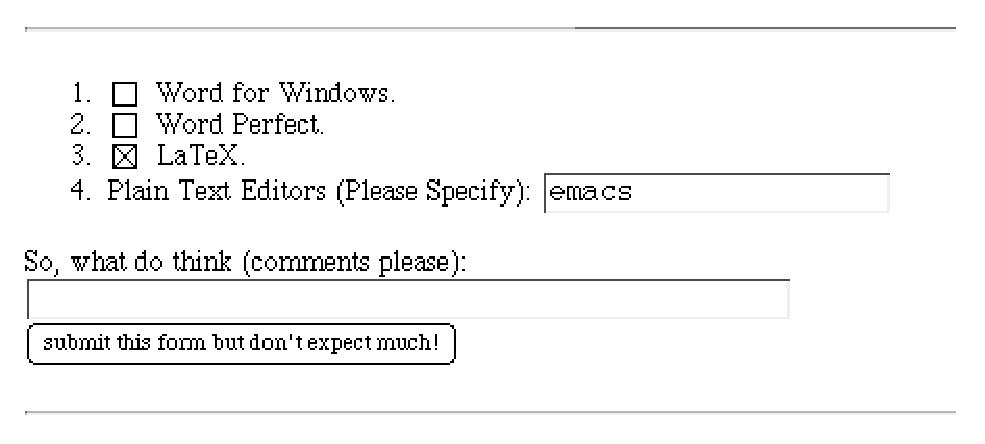
\includegraphics{psfiles/eform.ps}}}
    \end{center}
  \caption{An electronic form.
  In the online version the form would be active.}
  \label{eform}
\end{figure}
\end{latexonly}



\index{rawhtml@\Lc{rawhtml}}%
\paragraph*{\Lc{rawhtml}...\Lc{endrawhtml}\label{endrawhtml}}
\cbversion{97.1}\begin{changebar}
This is an alternative way to specify a chunk of raw \texttt{HTML} code,
using the old \AmS-style of delimiting environments.
Use of this style is discouraged; 
the \env{rawhtml} \htmlref{environment}{rawhtml} is preferred.%
\end{changebar}%

\index{comment@\env{comment} environment}%
\index{environment!comment@\env{comment}}%
\paragraph*{\Lc{begin\char123comment\char125}\label{comment}}
\cbversion{97.1}\begin{changebar}
This environment is simple for the convenience of ``commenting-out''
large sections of source code.
The contents of this environment is completely ignored,
both in the \LaTeX{} and \texttt{HTML} versions.
Such an environment is already used in \AmS-\LaTeX,
and perhaps with other packages.
It is defined here for its general utility.

\noindent
To insert \texttt{SGML}-style comments into the \texttt{HTML} files,
use the \env{rawhtml} environment as follows.
%begin{latexonly}
\begin{small}
%end{latexonly}
\begin{verbatim}
\begin{rawhtml}
<!--  this text is treated as a comment
      perhaps extending over several lines 
-->
\end{rawhtml}
\end{verbatim}
%begin{latexonly}
\end{small}
%end{latexonly}%
\end{changebar}%

\noindent
Note the \hyperref[page]{warning}{warning on page~}{}{env:warn}
concerning how the environment delimiters should be used in the
\LaTeX{} source code.


\index{latexonly@\Lc{latexonly}}%
\paragraph*{\Lc{comment...\char92endcomment}\label{endcomment}}
\cbversion{97.1}\begin{changebar}
This is an alternative way to specify a chunk of material intended
to be ignored in both the \LaTeX{} and \texttt{HTML} versions,
using the old \AmS-style of delimiting environments.
Use of this style (though convenient for typing) is discouraged,
since it is not as reliable as using the \env{comment} \htmlref{environment}{comment}.
\end{changebar}\html{\\}


\subsection{Arbitrary Tags and Attributes\label{sec:arbtags}}%
%\section{Arbitrary Tags and Attributes\label{sec:arbtags}}%
%
For version 97.1 of \latextohtml\ there is a new command which provides 
an extremely flexible way to include \texttt{HTML} 3.2 tags, along with
any values for the ``attributes'' of that tag, if desired.
\begin{quote}
\Lc{HTML}\verb|[|\Meta{attribs}\verb|]{|\Meta{tag}\verb|}|\label{HTMLtag}\\
\Lc{HTML}\verb|[|\Meta{attribs}\verb|]{|\Meta{tag}\verb|}{|\Meta{contents}\verb|}|
\end{quote}
When the \Meta{tag} also needs a closing tag (e.g \texttt{<I>...</I>})
the \Meta{contents} \emph{must} be given, enclosed in braces.
Both the opening and closing tags then will be placed correctly.


An important aspect of this is that any of the \Meta{tag},
\Meta{attribs} and \Meta{contents} may be given wholly
by expanding a \LaTeX{} macro, or may contain arbitrary macros, 
perhaps including other \Lc{HTML} commands.
\hyperref{The following table}{The contents of Figure~}{}{ex:HTML} 
was constructed using this feature; its \LaTeX{} source follows.

\HTML[50\% 3 noshade center]{HR}

\begin{htmlonly}
\begin{figure}
\begin{makeimage}
\end{makeimage}
\newcommand{\myalign}{center}
\newcommand{\mylist}{UL}
\newcommand{\myitem}[2]{\HTML[disc]{LI}{\simpletest{#1}{#2}}}
\newcommand{\simpletest}[2]{%
 \HTML{#1}{ a simple test of ``#2'',} using \HTML{CODE}{<#1>} .}
\newcommand{\tableopts}{10,border=5}

\newcommand{\tablelist}[4][\myalign]{\HTML[#1]{DIV}{
\HTML[\tableopts]{TABLE}{
\HTML[bottom]{CAPTION}{
#3
}\HTML{TR}{\HTML{TD}{
\HTML{#2}{
#4
}}}
}}\HTML[all]{BR}}

\tablelist[\myalign]{\mylist}{%
\textbf{A listing of the different text styles available in HTML 3.2}}{%
\myitem{B}{bold-face}
\myitem{I}{italics}
\myitem{TT}{teletype-text}
\myitem{U}{underlining}
\HTML[circle]{LI}{\simpletest{STRIKE}{strikeout}}
\myitem{EM}{emphasis style}
\myitem{STRONG}{strong style}
\myitem{CODE}{code style}
\myitem{CITE}{citation style}
\myitem{DFN}{definition style}
\HTML[square]{LI}{\simpletest{SAMP}{sample style}}
\HTML[square]{LI}{\simpletest{KBD}{keyboard style}}
\myitem{VAR}{variable style}}
%
 \caption{Example use of macros for raw \texttt{HTML} code.}
 \label{ex:HTML}
\end{figure}
\end{htmlonly}
%
\begin{latexonly}
\begin{figure}[ht]
\begin{center}
  \fbox{\scalebox{.7}{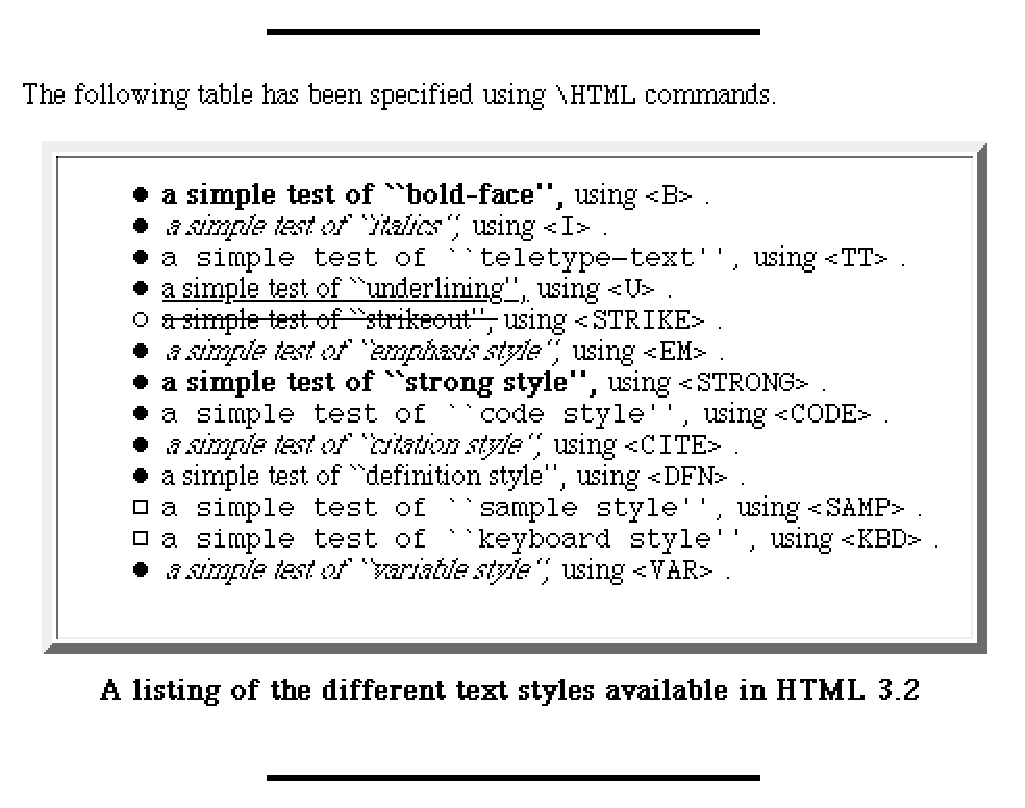
\includegraphics{psfiles/HTMLtab.ps}}}
 \caption{Example use of macros for raw \texttt{HTML} code.}
 \label{ex:HTML}
\end{center}
\end{figure}
\end{latexonly}

\HTML[50\% 3 noshade center]{HR}

%begin{latexonly}
\begin{small}
%end{latexonly}
\begin{verbatim}
\newcommand{\myalign}{center}
\newcommand{\mylist}{UL}
\newcommand{\myitem}[2]{\HTML[disc]{LI}{\simpletest{#1}{#2}}}
\newcommand{\simpletest}[2]{%
 \HTML{#1}{ a simple test of ``#2'',} using \HTML{CODE}{<#1>} .}
\newcommand{\tableopts}{10,border=5}

\newcommand{\tablelist}[4][left]{\HTML[#1]{DIV}{
\HTML[\tableopts]{TABLE}{
\HTML[bottom]{CAPTION}{
#3
}\HTML{TR}{\HTML{TD}{
\HTML{#2}{
#4
}}}
}}\HTML[all]{BR}}

\tablelist[\myalign]{\mylist}{%
\textbf{A listing of the different text styles available in HTML 3.2}}{%
\myitem{B}{bold-face}
\myitem{I}{italics}
\myitem{TT}{teletype-text}
\myitem{U}{underlining}
\HTML[circle]{LI}{\simpletest{STRIKE}{strikeout}}
\myitem{EM}{emphasis style}
\myitem{STRONG}{strong style}
\myitem{CODE}{code style}
\myitem{CITE}{citation style}
\myitem{DFN}{definition style}
\HTML[square]{LI}{\simpletest{SAMP}{sample style}}
\HTML[square]{LI}{\simpletest{KBD}{keyboard style}}
\myitem{VAR}{variable style}}
\end{verbatim}
%begin{latexonly}
\end{small}
%end{latexonly}

\HTML[50\% 3 noshade center]{HR}

\noindent
The above code demonstrates many aspects of the way \Lc{HTML}
commands can be used.
%
\begin{htmllist}\htmlitemmark{GreenBall}
\item [nesting: ] 
\Lc{HTML} commands can be nested to arbitrary depth.
%
\item [macros: ] 
Macros can be used to specify all or part of each argument.
%
\item [within macros: ] 
\Lc{HTML} commands work correctly within the expansions of other macros.
%
\item [attribute values: ]
Information within \Meta{attribs} can be specified in a very
loose way, as a comma-separated list of key/value pairs
or as single values. \\
Not even the commas are necessary: space(s), \Meta{tab}s 
or newlines are equally effective.
Indeed the horizontal rules preceding and following the table were 
specified by:
\begin{quote}
\begin{verbatim}
\HTML[50\% 3 noshade center]{HR}
\end{verbatim}
\end{quote}
%
\item [attribute names: ]
Usually it is \emph{not necessary} to know the names of the
attributes to the tags that are to be used. It is sufficient
just to give the values; these will be matched to the
appropriate attribute, according to the type of data required.
(If names are given, these are case-insensitive.)
%
\item [newlines: ] 
Although \LaTeX{} ignores linebreaks within the source code,
this is not so with \latextohtml. 
The strange spreading-out of the definition of the
\Lc{tablelist} command above was done with the purpose
solely of making the code in the resulting \texttt{HTML} files 
more easily readable, to a human.
(As most browsers ignore those newlines anyway, 
more compact code would have rendered the same on-screen.)
\end{htmllist}

\medskip\noindent
Some further aspects of the use of this \Lc{HTML}
command are not apparent from the above example. 

\begin{htmllist}\htmlitemmark{RedBall}
%
\item [invalid \Meta{tag}\,: ]
If a \Meta{tag} is specified that is not part of the 
\texttt{HTML} 3.2 specifications, then it and its attributes are 
not placed into the \texttt{HTML} document created by \latextohtml.
Any \Meta{contents} \emph{is} included as ordinary data; 
i.e. as text in paragraphs, etc.

\item [required attributes: ] 
Some tags have attributes which are required to have values,
if that tag is to be included in an \texttt{HTML} document.
Using the \Lc{HTML} command, if any such attribute
is not given an appropriate value then the tag is ignored.
Any \Meta{contents} are included in the document, 
as ordinary character data.

\item [valid HTML\,: ] 
Currently there is \emph{no} checking that the \Meta{contents}
of a \Meta{tag} contains only data (perhaps including other tags)
allowed by the DTD for \texttt{HTML} 3.2.
\begin{quote}
\textit{The requirement to produce valid \texttt{\upshape HTML} 
currently rests with the user.}
\end{quote}
This issue will be addressed in forthcoming revisions of \latextohtml.

\item [extra attributes and values: ]
The list of attributes for a \Meta{tag} can include
key-value pairs whose keys do not match any valid
attribute for the \Meta{tag}.
Such key-value pairs are simply ignored.
Similarly extra data values are ignored, 
as are values that do not match the
requirements for any valid attribute.

\item [attributes with similar data-types: ]
Several attributes to a \Meta{tag} may use values having 
the same or similar data-types. First any key-value pairs
are processed. Remaining values are allocated 
to those attributes which do not already have a value.
An ordering of the attributes is used, based on a perceived likelihood 
of each attribute being required to be changed from its default setting.

\end{htmllist}


\subsection{Conditional Text\label{sec:latexonly}}%
%\section{Conditional Text\label{sec:latexonly}}%
\tableofchildlinks*
\index{latexonly@\env{latexonly} environment}%
\index{htmlonly@\env{htmlonly} environment}%
\index{environment!htmlonly@\env{htmlonly}}%
\index{environment!latexonly@\env{latexonly}}%
\index{conditional text!scoped variant}\html{\\}%
\paragraph*{\Lc{begin\char123latexonly\char125} and 
\Lc{begin\char123htmlonly\char125}\label{latexonly}\label{htmlonly}}
Conditional text can be specified
using the environments \env{latexonly} and \env{htmlonly}. 
These allow writing parts of a document which are intended 
only for electronic delivery or only for paper-based delivery.

This would be useful for example in adding a long description of a
multi-media resource in the paper version of a document. 
Such a description would be redundant in the electronic version, 
as the user can have direct access to this resource. 

\medskip\goodbreak\noindent
Here is an example of the use of the \env{latexonly} environment,
used \hyperref[page]{earlier in}{on page~}{ of}{eform} this manual:
%begin{latexonly}
\begin{small}\indent
%end{latexonly}
\Lc{begin}\verb|{latexonly}|
\latex{\vskip-\baselineskip\vskip-\baselineskip}
\begin{verbatim}
\begin{figure}
    \begin{center}
    \fbox{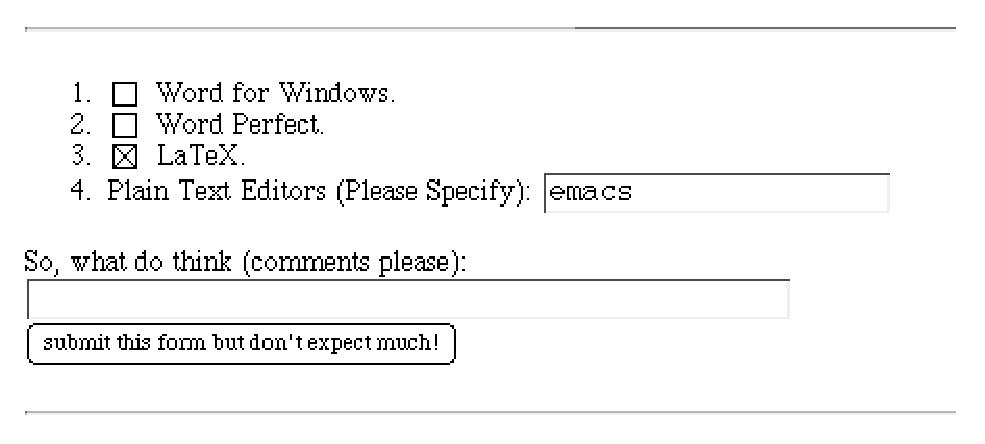
\includegraphics[width=4in]{psfiles/eform.ps}}
    \end{center}
    \caption{An electronic form. Of course in the online version of this
     document the form above would be active.}
\end{figure}
\end{verbatim}
\latex{\nobreak\vskip-\baselineskip\nobreak\indent\indent}%
\Lc{end}\verb|{latexonly}|
%begin{latexonly}
\end{small}\goodbreak\medskip
%end{latexonly}

\noindent
Note the \hyperref[page]{warning}{warning at the bottom of page~}{}{env:warn}
concerning how the environment delimiters should be used in the
\LaTeX{} source code.


\index{htmlonly@\Lc{htmlonly}}%
\paragraph*{\Lc{htmlonly...\char92endhtmlonly}\label{endhtmlonly}}
\cbversion{97.1}\begin{changebar}
This is an alternative way to specify a chunk of material intended
for the \texttt{HTML} version only,
using the old \AmS-style of delimiting environments.
Use of this style is discouraged; 
the \env{htmlonly} \htmlref{environment}{htmlonly} is preferred.%
\end{changebar}%


\index{latexonly@\Lc{latexonly}}%
\paragraph*{\Lc{latexonly...\char92endlatexonly}\label{endlatexonly}}
\cbversion{97.1}\begin{changebar}
This is an alternative way to specify a chunk of material intended
for the \LaTeX{} typeset version only,
using the old \AmS-style of delimiting environments.
Use of this style is discouraged; 
the \env{latexonly} \htmlref{environment}{latexonly} or the unscoped 
\htmlref{\texttt{\%begin\char123latexonly\char125}}{unlatexonly} 
construction are preferred.%
\end{changebar}%

\smallskip\noindent
Note the \hyperref[page]{warning}{warning at the bottom of page~}{}{env:warn}
concerning how the environment delimiters should be used in the
\LaTeX{} source code.


\index{conditional text!shorthand notation}%
\index{latex@\Lc{latex}}%
\index{html@\Lc{html}}%
\index{latexhtml@\Lc{latexhtml}}\html{\\}%
\paragraph*{\Lc{latex}, \Lc{html} and \Lc{latexhtml}\label{latexhtml}}
\cbversion{96.1}\begin{changebar}
There are also shorthand notations to accomplish the same thing 
as in the \env{latexonly} \htmlref{environment}{latexonly} and \env{htmlonly} 
\htmlref{environment}{htmlonly}, but with less typing.
\begin{itemize}
\item 
The \Lc{latex}\verb|{...}| command causes everything within the braces 
to be processed by \LaTeX, but ignored by \latextohtml.
\item  
Conversely, the \Lc{html}\verb|{...}| command causes everything within the braces 
to be ignored by \LaTeX{} and processed by \latextohtml.  
\item  
Finally the command \Lc{latexhtml}\verb|{...}{...}| causes everything 
within the first set of braces to be processed exclusively by \LaTeX, 
with the contents of the second set of braces processed solely by \latextohtml.%
\end{itemize}
\textbf{Warning: }
Only small pieces of text work reliably in this way. 
With whole paragraphs or contained sub-environments,
the ``conditional'' environments should be used instead.
\end{changebar}

\index{conditional text!without scope}%
\index{beginlatex@\texttt{\%{}begin\char123latexonly\char125}}%
\index{endlatex@\texttt{\%{}end\char123latexonly\char125}}%
\paragraph*{\texttt{\%begin\char123latexonly\char125}\label{unlatexonly}}
Another variant of the \env{latexonly} environment is available, 
in which everything between 
\verb|%|\verb|begin{latexonly}| and \verb|%|\verb|end{latexonly}| 
is ignored by \latextohtml.  
The difference is that the \env{latexonly} environment 
puts the contents into a group, in which all definitions are local.
There is no such scoping with the \verb|%begin...%end| variant,
since \LaTeX{} sees the initial \texttt{\%}s simply as starting comments.%

\medskip
\index{conditional text!example}\html{\\}\noindent
The following example should clarify what happens:
%begin{latexonly}
\begin{small}
%end{latexonly}
\begin{verbatim}
\newcommand{\A}{The letter A.}
\newcommand{\B}{The letter B.}
\end{verbatim}
\indent\indent\indent\verb|\|\verb|begin{latexonly}|\\
\indent\indent\verb|\renewcommand{\A}{Not the letter A.}|\\
\indent\indent\verb|\|\verb|end{latexonly}|\\
\indent\indent\verb|%|\verb|begin{latexonly}|\\
\indent\indent\verb|\renewcommand{\B}{Not the letter B.}|\\
\indent\indent\verb|%|\verb|end{latexonly}|
\begin{verbatim}
\begin{document}
\A \B
\end{document}
\end{verbatim}
%begin{latexonly}
\end{small}
%end{latexonly}
If you process this with \LaTeX, the result is: 
\quad\quad The letter A. Not the letter B.

\smallskip\noindent
Note the \hyperref[page]{warning}{warning at the bottom of page~}{}{env:warn}
concerning how the environment delimiters should be used in the
\LaTeX{} source code.

\medskip\index{conditional text!avoid using counters}\html{\\}\noindent
\textbf{Warning: }% 
Be careful when using \LaTeX{}  commands which alter the values of counters 
(e.g. numbered figures or equations) in conditional text, because this may 
cause the counter values in the electronic version to lose synchronisation 
with the values of the corresponding counters in the \LaTeX{} version.


\htmlrule[width=300]
\index{imagesonly@\env{imagesonly} environment}%
\index{environment!imagesonly@\env{imagesonly}}%
\paragraph*{\Lc{begin\char123imagesonly\char125}\label{imagesonly}}
\cbversion{97.1}\begin{changebar}
This environment is used to put \LaTeX{} code into the \fn{images.tex} file,
to be used when generating images. Typically this is used to add commands to
the preamble of \fn{images.tex}, such as setting the text or background color.
However code can be added at any other point as well; 
e.g. to change the background color of all images after a certain point in the document. 
\end{changebar}%

\smallskip\noindent
Note the \hyperref[page]{warning}{warning at the bottom of page~}{}{env:warn}
concerning how the environment delimiters should be used in the
\LaTeX{} source code.


\index{makeimage@\env{makeimage} environment}%
\index{environment!makeimage@\env{makeimage}}%
\paragraph*{\Lc{begin\char123makeimage\char125}\label{makeimage}}
\cbversion{97.1}\begin{changebar}
This is a special environment which forces an image to be made of its contents.
That is, one gets effectively a snapshot of a portion of a page
that has been typeset using \LaTeX. 
Within the normal \LaTeX{} typeset version of the document, this environment 
is completely transparent, adding its contents to the page as usual.

\index{makeimage@\env{makeimage} environment!inside@inside a \env{figure}}\html{\\}%
One further important use of the \env{makeimage} environment is as follows.
If a \env{makeimage} environment occurs as a sub-environment within 
a \env{figure} environment, then an image will \emph{not} be made of the
\env{figure}'s contents. Instead, the contents are treated as normal text,
each part being handled as if there were no \env{figure} at all,
except that everything is placed within a single cell of a
\HTMLtag{TABLE}...\HTMLtag{/TABLE} construction in \HTMLiii. 
The contents of any \Lc{caption}
commands are placed between \HTMLtag{CAPTION}...\HTMLtag{/CAPTION} tags 
for the \HTMLtag{TABLE}.

\index{makeimage@\env{makeimage} environment!empty sub-environment}\html{\\}%
Normally an image of the entire contents of the \env{figure} would be
placed within the single cell of the \HTMLtag{TABLE}.
Now images are made of any subparts of those \env{figure}'s contents 
that really need it, in particular the \env{makeimage} sub-environments.
An empty \env{makeimage} sub-environment does not generate an image of itself,
yet still it inhibits an image being made of the whole \env{figure}.
These comments apply also to \env{table} environments.
\end{changebar}\html{\\}




\subsection{Symbolic References shown as Hyperized Text\label{hyperized}%
%\section{Symbolic References shown as Hyperized Text\label{hyperized}%
\index{references@references\protect\label{IIIrefs}}}%
\tableofchildlinks*
\index{cross-references!|see{\htmlref{references}{IIIrefs}}}%
\index{references!symbolic\label{IIIsymref}}\index{symbolic labels|(}%
\index{references!numeric}%
\index{references!iconic}\html{\\}\noindent
In printed documents cross-references are shown 
through a \emph{numeric or symbolic indirection} 
e.g. ``see Figure 1'' (numeric indirection), 
or ``see section `Changes'~'' (symbolic indirection).  
\latextohtml{} can mirror this mechanism using the same numeric 
or symbolic references,
or when these are not appropriate by using iconic references.

\index{references!without indirection}%
\index{references!highlighted text}\html{\\}%
In a hypertext document however, cross-references can be shown 
without any indirection, just by highlighting a relevant piece of text. 
This can make a document more readable as it removes unnecessary
information. 

\index{hyperref@\Lc{hyperref}}%
\paragraph*{\Lc{hyperref}\label{hyperref}}
A single new \LaTeX{} command \Lc{hyperref} can be used for
specifying how a cross-reference should appear, 
both in the printed document and in the hypertext version.
For example, assuming that the label \verb|{sec:cond}|\label{sec:cond} 
is defined somewhere within a document, 
the command \Lc{hyperref}, taking 4 arguments,
can be used in that document as follows:
\index{hyperref@\Lc{hyperref}}%
\index{conditional text}%
%begin{latexonly}
\begin{small}
%end{latexonly}
\begin{verbatim}
\emph{Is the concept of
\hyperref
               % This will be highlighted in the hypertext version
{conditional text}			% argument #1
               % This will be shown in the printed version 
               % followed by a numeric reference ...      
{conditional text (see Section }  	% argument #2
               % ... followed by this text
{ for more information)} 		% argument #3
               % This is the common label 
{sec:cond}				% argument #4
a good idea? }
\end{verbatim}
%begin{latexonly}
\end{small}
%end{latexonly}

\noindent
Here is how it will be shown:
\begin{quote}
\emph{Is the concept of
\hyperref
% This will be highlighted in the hypertext version
{conditional text}
% This will be shown in the printed version  
% followed by a numeric reference ...      
{conditional text (see Section }  
% ... followed by this text
{ for more information)} 
% This the common label 
{sec:cond}
a good idea? }
\end{quote}

\begin{htmlonly}
In the printed version what would appear is:
\begin{quote}
\emph{Is the concept of conditional text (see Section 4.2 for more information) 
a good idea?}
\end{quote}
\end{htmlonly}

\begin{latexonly}%
In the hypertext version what would appear is:
\begin{quote}
\emph{Is the concept of \underline{conditional text} a good idea?}
\end{quote}
(Of course \underline{conditional text} would be an active hypertext link.)
\end{latexonly}

\bigskip\htmlrule[50\% center]
\cbversion{97.1}\begin{changebar}%
\noindent
An extended syntax for \Lc{hyperref} uses an optional argument, 
which determines what information is to be placed in the \LaTeX{} version
of the document. The value of this optional argument can also affect 
the number of required arguments. 
These forms are recognised:

%begin{latexonly}
\begin{small}
%end{latexonly}
\begin{quote}\label{hypernoref}
\Lc{hyperref}\verb|[ref]{|\Meta{HTML-text}\verb|}{|\Meta{LaTeX-text}%
\verb|}{|\Meta{post-LaTeX}\verb|}{|\Meta{label}\verb|}|\\
\Lc{hyperref}\verb|{|\Meta{HTML-text}\verb|}{|\Meta{LaTeX-text}%
\verb|}{|\Meta{post-LaTeX}\verb|}{|\Meta{label}\verb|}|\medskip

\Lc{hyperref}\verb|[pageref]{|\Meta{HTML-text}\verb|}{|\Meta{LaTeX-text}%
\verb|}{|\Meta{post-LaTeX}\verb|}{|\Meta{label}\verb|}|\\
\Lc{hyperref}\verb|[page]{|\Meta{HTML-text}\verb|}{|\Meta{LaTeX-text}%
\verb|}{|\Meta{post-LaTeX}\verb|}{|\Meta{label}\verb|}|\medskip

\Lc{hyperref}\verb|[noref]{|\Meta{HTML-text}\verb|}{|\Meta{LaTeX-text}%
\verb|}{|\Meta{label}\verb|}|\\
\Lc{hyperref}\verb|[no]{|\Meta{HTML-text}\verb|}{|\Meta{LaTeX-text}%
\verb|}{|\Meta{label}\verb|}|
\end{quote}
%begin{latexonly}
\end{small}
%end{latexonly}

\noindent
The first two are the defaults, where \LaTeX{} 
uses \Lc{ref}\verb|{|\Meta{label}\verb|}|.
With the next two \LaTeX{} uses \Lc{pageref}\verb|{|\Meta{label}\verb|}|,
while with the final two \LaTeX{} completely ignores the \Meta{label},
setting just the \Meta{LaTeX-text}.
\end{changebar}

\medskip
\index{hyperref@\Lc{hyperref}!pageref@\Lc{pageref} example}%
\html{\\}\noindent
For creating hyperlinks to other documents
using symbolic reference \Meta{label}s, 
see also the \Lc{externalref} 
\hyperref[page]{command}{command, described on page~}{}{externref}.

\medskip\noindent
The preceding paragraph is an example of the use of the \Lc{hyperref[page]} option.
Its source code is:
%begin{latexonly}
\begin{small}
%end{latexonly}
\begin{verbatim}
For creating hyperlinks to other documents
using symbolic reference \Meta{label}s, 
see also the \Lc{externalref} 
\hyperref[page]{command}{command, described on page~}{}{externref}.
\end{verbatim}
%begin{latexonly}
\end{small}
%end{latexonly}
\begin{htmlonly}
which appears in the \LaTeX{} typeset version as:
\begin{quote}
For creating hyperlinks to other documents
using symbolic reference \Meta{label}s, see also the
\Lc{externalref} command, described on page~31.
\end{quote}
\end{htmlonly}
\begin{latexonly}
which appears in the \texttt{HTML} version as:
\begin{quote}
For creating hyperlinks to other documents, using symbolic reference \Meta{label}s, 
see also the \Lc{externalref} \underline{command}.
\end{quote}
with the \underline{command} being an active hyperlink.
\end{latexonly}
\smallskip\noindent
In fact both \Lc{hyperref} and the \Lc{htmlref} command, to be described next,
permit textual hyperlinks based on symbolic \Meta{label}s from external files.


\index{htmlref@\Lc{htmlref}}%
\index{html.sty@\texttt{html.sty} style-file}
\paragraph*{\Lc{htmlref}\label{htmlref}}
Another command also defined in \fn{html.sty} is \Lc{htmlref} 
which has the same effect as \Lc{hyperref}
during the conversion to \texttt{HTML}.
It takes two arguments, some text and a label. 
In the \texttt{HTML} version the
text will be ``hyperized'', pointing to the label. 
In the paper version the text will be shown as it is 
and the label will be ignored; e.g.
%
\index{htmlref@\Lc{htmlref}!easy to make links}%
%begin{latexonly}
\begin{small}
%end{latexonly}
\begin{verbatim}
With \verb|\htmlref| \htmlref{it's easy to make links}{fig:example}.
\end{verbatim}
%begin{latexonly}
\end{small}
%end{latexonly}
which produces:
\begin{quote}
With \Lc{htmlref} \htmlref{it's easy to make links}{fig:example}.
\end{quote}
\begin{htmlonly}
In the \LaTeX{} typeset version it will appear simply as:
\begin{quote}
With \Lc{htmlref} it's easy to make links.
\end{quote}
\end{htmlonly}
\begin{latexonly}
In the \texttt{HTML} version it is shown as:
\begin{quote}
With \Lc{htmlref} \underline{it's easy to make links}.
\end{quote}
\end{latexonly}
\html{\\}
\goodbreak

\subsection{Hypertext Links in Bibliographic References (Citations)}%
%\section{Hypertext Links in Bibliographic References (Citations)}%
\tableofchildlinks*
\index{references!bibliographic}\index{bibliography|(}%
\index{bibliography!bibliographic database}%
\index{bibliography!using .bib@using \texttt{.bib} file}\html{\\}%
If a report or a book that is cited (using the \Lc{cite} command) 
is available (or there is information about it) on the World-Wide
Web, then it is possible to add the appropriate hypertext links
in your bibliographic database (the \texttt{.bib}) file. 

\bigskip
\index{bibliography!example using URLs}%
\index{bibliography!string commands@\texttt{\char64 string} commands}%
\index{LaTeX blue book@\LaTeX{} blue book}\html{\\}%
\noindent
Here is an example of a bibliographic entry for the original
\LaTeX{} \cite{lamp:latex} blue book:\nobreak
%begin{latexonly}
\begin{small}
%end{latexonly}
\begin{verbatim}
@string{curiaURL="\htmladdnormallink
{http://curia.ucc.ie/info/TeX/menu.html}
{http://curia.ucc.ie/info/TeX/menu.html}"}

@string{fernURL="\htmladdnormallink
{http://es-sun2.fernuni-hagen.de/info2html?(latex.info)Top}
{http://es-sun2.fernuni-hagen.de/info2html?(latex.info)Top}"}

@book{lamp:latex,
title = "LaTeX User's Guide \& Reference Manual, 2nd edition",
year = 1994 ,
author = "Leslie Lamport",
Publisher = "Addison--Wesley Publishing Company, Inc.",
note = "Online information on {\TeX} and {\LaTeX} is available at "
 # curiaURL # " and " # fernURL }
\end{verbatim}
%begin{latexonly}
\end{small}
%end{latexonly}
See the \htmlref{bibliography}{biblio} for how this will appear.\html{\\}
No other modifications are required; \LaTeX{} and Bib\TeX{} should work as normal.
%
\index{bibliography!string commands@\texttt{\char64string} commands}%
\cbversion{96.1f}\begin{changebar}
Note that it would be sensible to put the \texttt{@string} commands
into a separate file, \fn{urls.bib} say, 
loaded with the main file via\html{\\} \verb|\bibliography{urls,...}|.%
\end{changebar}

\smallskip\index{citations!Harvard style}%
\index{bibliography!Harvard style}\label{harvard}\html{\\}%
\noindent
For those who use the Harvard style for references
\htmladdnormallinkfoot{there exists a special conversion add-on package}%
{http://www.arch.su.edu.au/\~{}peterw/latex/harvard/}.

\index{citations!natbib@\env{natbib} package}%
\index{bibliography!natbib@\env{natbib} package}%
\index{citations!Harvard style!handled@handled by \env{natbib}}%
\cbversion{96.1g}\begin{changebar}
The \env{natbib} package, written for \LaTeX{} by \PatrickDaly,
provides even more flexibility in the way a reference may be cited. 
All the features of \htmlref{this package}{natbib} are implemented 
for \latextohtml{} via the \fn{natbib.perl} file.
(Indeed there is even a mode whereby \env{natbib} handles
the Harvard style of citation. 
This requires loading also the \env{nharvard} \htmlref{package}{nharvard}.)

\medskip
\noindent\textbf{Thanks...} to \Wilck\ for the bulk of the work 
in producing this extension, and to \RossMoore\ for 
necessary adjustments to allow it to work correctly with the 
\htmlref{document segmentation strategy}{Segmentation}.
\end{changebar}


\index{hypercite@\Lc{hypercite}}%
\paragraph*{\Lc{hypercite}\label{hypercite}}
\cbversion{97.1}\begin{changebar}
Analogous to \Lc{hyperref} is the \Lc{hypercite} command,
which allows a free-form textual hyperlink to the bibliography,
whereas the \LaTeX{} typeset version contains the usual citation code.
The allowed syntax is as follows.
%begin{latexonly}
\begin{small}
%end{latexonly}
\begin{quote}
\Lc{hypercite}\verb|[int]{|\Meta{HTML-text}\verb|}{|\Meta{LaTeX-text}%
\verb|}{|\Meta{opt-LaTeX}\verb|}{|\Meta{label}\verb|}|\\
\Lc{hypercite}\verb|[cite]{|\Meta{HTML-text}\verb|}{|\Meta{LaTeX-text}%
\verb|}{|\Meta{opt-LaTeX}\verb|}{|\Meta{label}\verb|}|\\
\Lc{hypercite}\Meta{HTML-text}\verb|}{|\Meta{LaTeX-text}%
\verb|}{|\Meta{opt-LaTeX}\verb|}{|\Meta{label}\verb|}|\medskip

\Lc{hypercite}\verb|[nocite]{|\Meta{HTML-text}\verb|}{|\Meta{LaTeX-text}%
\verb|}{|\Meta{label}\verb|}|\\
\Lc{hypercite}\verb|[no]{|\Meta{HTML-text}\verb|}{|\Meta{LaTeX-text}%
\verb|}{|\Meta{label}\verb|}|\\
\Lc{hypercite}\verb|[ext]{|\Meta{HTML-text}\verb|}{|\Meta{LaTeX-text}%
\verb|}{|\Meta{label}\verb|}|
\end{quote}
%begin{latexonly}
\end{small}
%end{latexonly}
The first three forms are equivalent; 
\LaTeX{} uses \Lc{cite}\verb|[|\Meta{opt-LaTeX}\verb|]|\Meta{label}\,,
after placing the \Meta{LaTeX-text}.
Note that \verb|{|\Meta{opt-LaTeX}\verb|}| \emph{must} be specified, 
even if empty `\verb|{}|'.

Similarly the latter three forms are equivalent, 
with \LaTeX{} using \Lc{nocite}\verb|{|\Meta{label}\verb|}|\,, 
to force the particular reference to appear on the bibliography page, 
even though no explicit marker is placed at this point.
(Thus there is no need for an optional  \Meta{opt-LaTeX} argument.)\html{\\}
Within the \texttt{HTML} version a hyperlink is produced when the \Meta{HTML-text} 
is not empty. External label files are also searched, 
in order to match the symbolic \Meta{label}, see also 
\hyperref[page]{\Lc{externalcite}}{\Lc{externalcite} on page~}{}{externcite}.

\smallskip\noindent\label{hyperciteXmpl}%
\index{hypercite@\Lc{hypercite}!example}%
\index{htmlcite@\Lc{htmlcite}!example}\html{\\}\noindent
\htmlref{Earlier}{hypcites} in this manual the following source code was used:
%begin{latexonly}
\begin{small}
%end{latexonly}
\begin{verbatim}
commands described in the \LaTeX{} \htmlcite{blue book}{lamp:latex}, 
...
as well as many other \LaTeX{} constructions, such as are described in 
the \LaTeX{} \hypercite{\emph{Companion}}{\emph{Companion}}{}{goossens:latex} 
and \LaTeX{} \hypercite{\emph{Graphics Companion} (e.g. \Xy-pic)}%
{\emph{Graphics Companion}}{\Xy-pic}{goossens:latexGraphics};
\end{verbatim}
%begin{latexonly}
\end{small}
%end{latexonly}
which produces:
\begin{quote}
commands described in the \LaTeX{} \htmlcite{blue book}{lamp:latex}, 
\\~~...\\
as well as many other \LaTeX{} constructions, such as are described in 
the \LaTeX{} \hypercite{\emph{Companion}}{\emph{Companion}}{}{goossens:latex} 
and \LaTeX{} \hypercite{\emph{Graphics Companion} (e.g. \Xy-pic)}%
{\emph{Graphics Companion}}{\Xy-pic}{goossens:latexGraphics};
\end{quote}
\begin{latexonly}
whereas in the \texttt{HTML} version one sees:
\begin{quote}
commands described in the \LaTeX{} \underline{blue book}, 
\\~~...\\
as well as many other \LaTeX{} constructions, 
such as are described in the \LaTeX{} \underline{\emph{Companion}} 
and  \LaTeX{} \underline{\emph{Graphics Companion} (e.g. \Xy-pic)};
\end{quote}
\end{latexonly}
%
\begin{htmlonly}
whereas in the \LaTeX{} typeset version one sees:
\begin{quote}
commands described in the \LaTeX{} blue book,\\
~~...\\
as well as many other \LaTeX{} constructions, such as are described in the \LaTeX{} 
\textit{Companion}[2] and \LaTeX{} \textit{Graphics Companion}[3, \Xy-pic];
\end{quote}
\end{htmlonly}
\end{changebar}%


\index{htmlcite@\Lc{htmlcite}}%
\paragraph*{\Lc{htmlcite}\label{htmlcite}}
\cbversion{97.1}\begin{changebar}
Analogous to \Lc{htmlref} is the \Lc{htmlcite} command,
which creates a textual hyperlink to a place on the document's bibliography page, 
but without displaying any reference marker in the \LaTeX{} typeset version.
(See \htmlref{above}{hyperciteXmpl} for an example.)%

The \Lc{externalcite} 
\hyperref[page]{command}{command, described on page~}{, }{externcite}
provides a similar facility when the bibliography page is ``external'';
that is, not part of the current document.%
\end{changebar}

\index{bibliography|)}



\subsection{Symbolic References between Living Documents\label{external_cross}}%
%\section{Symbolic References between Living Documents\label{external_cross}}%
\tableofchildlinks*
\index{external references|(}
\index{references!to external documents}%
\index{references!symbolic}%
\index{symbolic labels!see also@\emph{see also} 
 \htmlref{references, symbolic}{IIIsymref}}%
\index{labels!symbolic}%
%
\cbversion{96.1}\begin{changebar}
The method of the previous section to generated
symbolic \htmlref{hyperized}{hyperized} links can
easily be extended to \emph{external} documents processed by \latextohtml.  
When \latextohtml{} processes a document, it generates a \Perl{} file 
named \Meta{prefix}\fn{labels.pl}
which contains a list of all the symbolic labels that were defined, 
along with their locations.  
The \htmlref{\Meta{prefix}}{prefix} is empty unless otherwise specified, 
to allow different document segments to share the same directory.  
\end{changebar}

\index{externallabels@\Lc{externallabels}}%
\index{externalref@\Lc{externalref}}%
\paragraph*{\Lc{externallabels}\label{externlabels}}
\cbversion{96.1}\begin{changebar}
Links to an external document are then possible once a connection 
is established to that document's \fn{labels.pl} file.  
This connection is established by the \Lc{externallabels} command:%
\end{changebar}%
%
\begin{quote}
%begin{latexonly}
\begin{small}
%end{latexonly}
\Lc{externallabels}\verb|{|\Meta{URL to directory of external document}\verb|}|\\
\verb|               {|\Meta{local copy of external document labels.pl file}\verb|}|
%begin{latexonly}
\end{small}
%end{latexonly}
\end{quote}
%
\index{labels!external}\html{\\}%
The first argument to \Lc{externallabels} should be a URL to 
the directory containing the external document.  
The second argument
should be the full path-name to the \fn{labels.pl} file belonging
to the external document.  Note that for \emph{remote} external documents
it is necessary to copy the \fn{labels.pl} file locally so that it
can be read when processing a local document that uses it.
The command \Lc{externallabels} can be used once for each external
document in order to import the \textit{external labels}\label{externallabels}
into the current document.
A warning is given if \fn{labels.pl} cannot be found.

\begin{changebar}%
If a symbolic reference made in either of the commands described
\hyperref{on the previous page}{in Section~}{}{hyperized} is not 
defined within the document itself,
\latextohtml{} will look for that reference in one of the external
files\footnote{Care must be taken to ensure that critical symbolic
references are unique across related documents.}.
After any modifications in an external document 
(sections added/deleted, segmentation into different physical parts, etc.) 
a new \fn{labels.pl} will be generated.  
If the \Lc{externallabels} command in another 
document contains the correct address to an updated copy of
the \fn{labels.pl} file, then the cross-references will be re-aligned
after running the local document through the translator.

\index{labels!internal}\label{internallabels}\html{\\}%
There is also a mechanism analogous to the
\textit{label--ref} pairs of \LaTeX, which can be used only 
within a single document. 
These labels are called \textit{internal labels},
as opposed to the \htmlref{external labels}{externallabels} defined above.
They are used extensively with the document segmentation strategy
described \hyperref{later}{in Section~}{}{Segmentation}.

Either type of label is defined with a \LaTeX{} \Lc{label} command.  
Labels can be referenced \textit{within} a document using a \Lc{ref} command.
When processed by \LaTeX, each \Lc{ref} command is replaced by the 
section number in which the corresponding \Lc{label} occurred.
When processed by the translator, each \Lc{ref} is replaced by 
a hypertext link to the place where the corresponding \Lc{label} occurred.%
\end{changebar}%
 

\index{references!to external documents}%
\index{externalref@\Lc{externalref}}%
\paragraph*{\Lc{externalref}\label{externref}}
\begin{changebar}%
This mechanism can be extended to external documents:
\begin{quote}
%begin{latexonly}
\begin{small}
%end{latexonly}
\Lc{externalref}\verb|{|\Meta{symbolic label in remote document}\verb|}|
%begin{latexonly}
\end{small}
%end{latexonly}
\end{quote}
The argument to \Lc{externalref} may be any symbolic label defined 
in the \fn{labels.pl} file of any of the external documents.
Such references to external symbolic labels are then translated
into hyper-links pointing to the external document.%
\end{changebar}%


\index{citations!within external bibliographies}%
\index{externalcite@\Lc{externalcite}}%
\paragraph*{\Lc{externalcite}\label{externcite}}
\cbversion{97.1}\begin{changebar}
%
Analogous to \htmlref{\Lc{externalref}}{externref},
the \Lc{externalcite} command is used to create a citation link,
where the bibliography page is not part of the current document.
As with \Lc{externalref} symbolic labels for the bibliography page
must have been loaded using 
\htmlref{\Lc{externallabels}}{externlabels}.

A particularly important use for this is in allowing multiple documents 
to access information in a common bibliographic listing.
For example: all of an author's publications; 
a comprehensive listing of publications in a particular field; 
the (perhaps yearly) output of publications 
from a particular organisation or institution.

\medskip\noindent
\textbf{Thanks...} to \Engberg\ for suggesting this feature.
\end{changebar}

\index{external references|)}


\subsubsection{Cross-Referencing Example\label{crossrefs}}% 
%\subsection{Cross-Referencing Example\label{crossrefs}}% 
To understand this mechanism better consider 
how you would maintain a link to this section  
(of the hypertext version of this document) from one of your documents,
without using labels.
Sure enough you can get the name of the physical file that this section is in. 
This however is quite likely to change, and any links to it would become invalid. 
\index{link validation!done by hand}%
To update your link, the name of the new file must be found 
and your link changed by hand. 
Also there is no general updating mechanism, so the only way to find
out if your document is pointing to the right place is by actually
following the link, then doing a manual update\footnote{%
Link validation can be done automatically but the updating must be done
manually when filenames have changed (assuming no other symbolic label
mechanism is available).}.

\index{link validation!symbolic labels}\html{\\}%
Next consider how it could be done with symbolic labels. 
First you have to import the labels used in this document 
by copying the file \htmladdnormallink{\fn{labels.pl}}
{http://cbl.leeds.ac.uk/nikos/tex2html/doc/manual/labels.pl},
saving it in \path{/tmp/labels.pl} say,
then adding anywhere in your document:
%begin{latexonly}
\begin{small}
%end{latexonly}
\begin{verbatim}
\externallabels{http://cbl.leeds.ac.uk/nikos/tex2html/doc/manual}%
               {/tmp/labels.pl}
\end{verbatim}
%begin{latexonly}
\end{small}
%end{latexonly}
After that you can use the label `\texttt{crossrefs}' defined at the beginning of this 
section\footnote{You either have to guess the role of each label by
looking at the \fn{labels.pl} file or by asking the author!} as follows:
%begin{latexonly}
\begin{small}
%end{latexonly}
\begin{verbatim}
\externalref{crossrefs}
\end{verbatim}
%begin{latexonly}
\end{small}
%end{latexonly}
This will be translated into the appropriate hyper-link to this page.
If there are any changes in this document and you would like to
bring your document up-to date, you have to copy 
\htmladdnormallink{\fn{labels.pl}}%
{http://cbl.leeds.ac.uk/nikos/tex2html/doc/manual/labels.pl} again
and rerun the translator on your document. Of course if I move the 
directory containing the \texttt{HTML} files for this document somewhere else, 
then you would have to make a change in the argument of the 
\Lc{externallabels} command to reflect this. 

\index{references!collaboration required}%
It is obvious that some level of collaboration is required between
authors trying to maintain cross-references between different documents. 
Using symbolic labels makes this a lot easier 
(especially for documents written by the same author).
\index{symbolic labels|)}



\subsection{Miscellaneous commands for \texttt{HTML} effects\label{misceffects}}%
%\section{Miscellaneous commands for \texttt{HTML} effects\label{misceffects}}%
\tableofchildlinks*
\index{html.sty@\texttt{html.sty} style-file}%

\noindent
The \env{html} package, through the \LaTeX{} input file \fn{html.sty},
and its \Perl{} counterpart \fn{html.perl}, implements several 
new commands that are intended entirely for effects within the
produced \texttt{HTML} files. In \LaTeX{} these commands, their arguments,
and any optional arguments are completely ignored.

\index{htmlrule@\Lc{htmlrule}}%
\index{visual separation!using \Lc{htmlrule}}%
\paragraph*{\Lc{htmlrule } and 
 \Lc{htmlrule*}\label{htmlrule}}
One such device provided by \fn{html.sty},
is the \Lc{htmlrule} command. 
This puts a horizontal rule into the \texttt{HTML} file only;
being ignored in the \texttt{.dvi} version. 
It is useful to provide extra visual separation between paragraphs,
without creating a new \texttt{HTML} page, 
such as might warrant extra vertical space within the printed version.

\index{htmlrule!htmlrulestar@\Lc{htmlrule*}}%
\index{htmlrule!variants}%
\index{htmlrule!attributes@attributes to the \HTMLtag{HR} tag}%
\cbversion{97.1}\begin{changebar}
Much variation can be obtained in the horizontal rule that is produced,
using extended forms of the \Lc{htmlrule} command:
\begin{quote}
%begin{latexonly}
\begin{small}
%end{latexonly}
\Lc{htmlrule}\\
\Lc{htmlrule*}\\
\Lc{htmlrule[}\Meta{attribs}\texttt{]}\\
\Lc{htmlrule*[}\Meta{attribs}\texttt{]}
%begin{latexonly}
\end{small}
%end{latexonly}
\end{quote}
Whereas a ``break'' tag \HTMLtag{BR} normally precedes the \HTMLtag{HR} generated
by the \Lc{htmlrule} command, 
this break is omitted when using the \Lc{htmlrule*} variant. 

\htmlrule[center,width=200]

\noindent
Furthermore, the optional argument \Meta{attribs} can be used to specify 
attributes for \emph{both} the \HTMLtag{HR} and \HTMLtag{BR} tags. 
More specifically, \Meta{attribs} should be a list of attribute-names 
and/or key-value pairs \texttt{\Meta{key}=\Meta{value}} separated by spaces or commas. 
This list is parsed to extract those attributes applicable to the \HTMLtag{HR} tag,
and those applicable to the \HTMLtag{BR} (with the unstarred variant).

\medskip\htmlrule[right,width=200,size=5]
\noindent
Using \HTMLiii, this allows variations to be specified for:
\begin{itemize}
\item 
the (vertical) thickness of the horizontal line in pixels: \texttt{SIZE=\Meta{num}};
\item 
the (horizontal) width of the line in pixels or points: \texttt{WIDTH=\Meta{width}};
\item 
alignment: \texttt{WIDTH=\char34...\char34 } 
taking \texttt{left}, \texttt{right} or \texttt{center};
\item 
removal of the shadowed effect \texttt{NOSHADE};
\item 
positioning of the rule with respect to text-flows: 
\texttt{CLEAR=\char34...\char34 } 
taking \texttt{left}, \texttt{all}, \texttt{right} or \texttt{none}. 
\htmlrule[right,width=200,size=5]
\end{itemize}%
Some examples of these effects appear on 
\latex{the \texttt{HTML} version of} this page.%
\end{changebar}%


\index{strikeout@\Lc{strikeout}}%
\paragraph*{\Lc{strikeout\char123}\Meta{text}\texttt{\char125}\label{strikeout}}
\cbversion{97.1}\begin{changebar}
With this command the \Meta{text} is processed as normal in the \texttt{HTML} version,
then placed between \HTMLtag{STRIKE}...\HTMLtag{/STRIKE} tags.
Thus a horizontal line should be drawn through the middle of the \Meta{text}.\html{\\}
Currently the command and the \Meta{text} are ignored in the \LaTeX{} version.%
\end{changebar}%


\index{tableofchildlinks@\Lc{tableofchildlinks}}%
\paragraph*{\Lc{tableofchildlinks }\label{tochlinks}}
\cbversion{97.1}\begin{changebar}
As an extra aid to navigation within a long page, 
containing several (sub)subsections or deeper levels of sectioning,
there is the \Lc{tableofchildlinks} command.
This does not generate anything new, for a table of the child links
on or from a page is generated automatically by \latextohtml.

However if this command, or its variant \Lc{tableofchildlinks*},
occurs within the source code to appear on a particular \texttt{HTML} page,
then the child-links table will be placed at that point
where the command occurs. 
Normally a break tag \HTMLtag{BR} is inserted to separate the table of child-links 
from the surrounding text. The \Lc{tableofchildlinks*} omits this extra break
when it would result in too much space above the table.

For example throughout this section of the \latex{\texttt{HTML} version of the }manual, 
all subsections in which several explicit commands have been discussed
have their child-links table placed at the top of the page,
using \Lc{tableofchildlinks*}. 
This helps to quickly find the description of how the commands are used.%
\end{changebar}%


\index{htmlinfo@\Lc{htmlinfo}}%
\paragraph*{\Lc{htmlinfo }\label{htmlinfo}}
\cbversion{97.1}\begin{changebar}
Normally an ``About this document...'' page is created at the end
of the \texttt{HTML} document, containing technical information
about how the document was created, by whom, or any other information
contained in the \fn{\$INFO} \htmlref{variable}{infostring}.
This information can be made to appear at any other place within the document 
by specifying \Lc{htmlinfo} at the desired place in the source.
For example, the information may be best suited for the title-page.

The variant \Lc{htmlinfo*} places the information, but leaves out the 
standard ``About this document...'' header. 
Instead the \htmlref{\Lc{htmlhead}}{htmlhead} command 
can be used to place an alternative heading, prior to the \Lc{htmlinfo*} command.
Neither this heading nor the \fn{\$INFO} \htmlref{contents}{infostring} appears 
in the \LaTeX{} typeset version.%
\end{changebar}%


\index{bodytext@\Lc{bodytext}}%
\paragraph*{\Lc{bodytext\char123}\Meta{options}\texttt{\char125}\label{bodytext}}
\cbversion{96.1g}\begin{changebar}
The text and background colors, and colors for the text of hypertext links can
be set on an \texttt{HTML} page by giving appropriate attributes 
with the \HTMLtag{BODY ...} tag. This is particularly easy to do
using the \Lc{bodytext} command, 
which simply inserts the \Meta{code} as the desired list of attributes.%

\medskip
\index{bodytext@\Lc{bodytext}!no checking for valid attributes}\html{\\}%
\noindent
\textbf{Warning: }Any previous settings for the \HTMLtag{BODY ...} tag
are discarded. Furthermore no checking is done to verify whether the given \Meta{options}
indeed contains a list of attributes and values valid for the \HTMLtag{BODY ...} tag.\html{\\}
When using \Lc{bodytext} you are assumed to know precisely what you are doing!

\medskip\noindent
Other packages contain commands which alter the contents of the \HTMLtag{BODY ...} tag;
notably the \fn{color.perl} implementation of \LaTeX's \env{color} package,
and the (prototype) \env{frames} package, by \Wilck\ and \RossMoore.
In both these packages the requested information is checked for
validity as an attribute within the \HTMLtag{BODY ...} tag.
\end{changebar}%

\index{htmlbody@\Lc{htmlbody}}%
\paragraph*{\Lc{htmlbody\char123}\Meta{options}\texttt{\char125}\label{htmlbody}}
\cbversion{97.1}\begin{changebar}
This is similar to the \Lc{bodytext} command, except that it adds the
value of an attribute, or allows an existing value to be changed.
Thus it can be used to alter just a single one of the text and background colors, 
colors for the text of hypertext links or add a background pattern.
The \Meta{options} are given as key-value pairs; some checking is done to ensure 
the validity of the attributes whose values are being set.%
\end{changebar}%

\index{htmlbase@\Lc{htmlbase}}%
\paragraph*{\Lc{htmlbase\char123}\Meta{URL}\texttt{\char125}\label{htmlbase}}
\cbversion{96.1g}\begin{changebar}
This specifies that the given \Meta{URL} be included in the \HTMLtag{HEAD} section
of each \texttt{HTML} page via a tag: 
\texttt{<BASE HREF=\char34\Meta{URL}\char34}.\html{\\}
Such a feature is particularly useful\dots 
\begin{itemize}
\item
when preparing a document whose final location may be different from where it was created; 
By making all internal references be relative (to the the provided \Meta{URL}),
a whole directory tree containing the document 
and all its subparts can be moved to elsewhere.
A single edit in each \texttt{HTML} file produces the complete document intact 
at the new location.
%
\item
by allowing just single page to be copied to another location, but act as if it were
part of the original document (provided this is accessible across the Web).
Relative URLs within the copied page are relative to the base \Meta{URL},
rather than relative to the new location.
%
\item
Other uses for this feature are likely to become apparent.%
\end{itemize}\end{changebar}%


\index{HTMLset@\Lc{HTMLset}!alters a \Perl{} variable}%
\index{HTMLset@\Lc{HTMLsetenv}!alters a \Perl{} variable}%
\paragraph*{\Lc{HTMLset\char123}\Meta{which}\texttt{\char125\char123}%
\Meta{value}\texttt{\char125} and 
\Lc{HTMLsetenv\char123}\Meta{which}\texttt{\char125\char123}%
\Meta{value}\texttt{\char125}\label{HTMLset}}
\cbversion{97.1}\begin{changebar}
The \Lc{HTMLset} command provides a mechanism whereby an arbitrary
\Perl{} variable can be assigned a value dynamically, during the \latextohtml{} processing. 
A variable having name `\texttt{\$}\Meta{which}' is assigned the specified \Meta{value},
overwriting any value that may exist already. The \Lc{HTMLsetenv} is for the same purpose,
but it is expanded in order as if it were an environment, rather than a command.

\medskip\noindent
\textbf{Warning: }This is intended for \Perl{} programmers only.
Use this command at your own risk!
\end{changebar}

\htmlrule[width=300]
\index{LaTeX2HTML@\latextohtml{}!command for its name}%
\index{names of important packages}%
\index{latextohtml@\Lc{latextohtml}!gives @gives \latextohtml{}}%
\paragraph*{\Lc{latextohtml}\label{l2hname}} 
\cbversion{97.1}\begin{changebar}
expands to the name \latextohtml, of this translator.
Commands for parts of names of important \LaTeX{} packages are also 
included with \latextohtml: e.g. \TeX, \LaTeX, \AmS, \Xy\,.
(This is to make it easy to refer to these products, in a consistent way
within the \texttt{HTML} pages; you may still need \LaTeX{} definitions
for the typeset version.)
\end{changebar}
\medskip



\subsection{Active Image Maps\label{ImageMaps}}%
%\section{Active Image Maps\label{ImageMaps}}%
\index{images!image-maps|(}\index{image-map!map-file}%
\index{HTML@\texttt{HTML}!Version 3.2}%
\index{usemap@\texttt{usemap}}%
\index{thumbnail}%
\cbversion{96.1}\begin{changebar}%
\emph{Image maps} are images with active regions in which a 
Web-surfer can click, to send him off to another sector of cyberspace.  
\latextohtml{} can design either inline ``figures'' or external ones 
(with or without a thumbnail version) to be image-maps.  
However \texttt{HTML} requires a URL of a \texttt{HTML} \emph{map-file}, 
which associates the coordinates of each active region in
the map with a destination URL.  
Usually this map file is kept on the server machine, 
however \texttt{HTML} 3.2 also allows it 
to reside on the \htmladdnormallink{client side}%
{http://ds.internic.net/internet-drafts/draft-seidman-clientsideimagemap-02.txt} 
for faster response.  
Both configurations are supported by \latextohtml{} 
through the \Lc{htmlimage} options
`\texttt{map=}' and `\texttt{usemap=}' respectively.

\index{makemap@\texttt{makemap}}%
\index{image-map!user-map file}\html{\\}%

Keeping such a map file up to date manually can be tedious, 
especially with dynamic documents under revision.
An experimental program \fn{makemap} helps automate this process.  
This program (which is really a \Perl{} script)
takes one mandatory argument and an optional argument.
The mandatory argument is the name of a \emph{user-map} file,
defined below.  The optional argument is the name of the
directory where the \texttt{HTML} map file(s) are to be placed.

\index{image-map!example}\html{\\}%
The best way of describing how this works is by example.
Suppose a document has two figures designated to
become active image-maps.  The first
figure includes a statement like:
%begin{latexonly}
\begin{small}
%end{latexonly}
\begin{verbatim}
\begin{figure}
\htmlimage{map=/cgi-bin/imagemap/BlockDiagram.map,...}
. . .
\end{figure}
\end{verbatim}
%begin{latexonly}
\end{small}
%end{latexonly}
The second figure has a line like:

%begin{latexonly}
\begin{small}
%end{latexonly}
\begin{verbatim}
\begin{figure}
\htmlimage{map=/cgi-bin/imagemap/FlowChart.map,...}
. . .
\end{figure}
\end{verbatim}
%begin{latexonly}
\end{small}
%end{latexonly}

\medskip\htmlrule[50\% center]
\index{image-map!CERN server}\index{CERN!image-map server}%
\index{image-map!NCSA server}\index{NCSA!image-map server}%
\index{image-map!example}\html{\\}%
\noindent
A typical user-map file, named \fn{report.map}, 
might contain the following information\footnote{%
This file is designed for an \appl{NCSA} server.  
\appl{CERN} servers use ``\texttt{rect}''
instead of ``\texttt{rectangle},'' 
specify a radius instead of an outer point in the circle, 
and enclose point coordinates by parentheses.}:
%begin{latexonly}
\begin{small}
%end{latexonly}
\begin{verbatim}
#
#  Define the location(s) of the labels.pl file(s):
#
+report/ <URL>
#
#  Define map #1:
#
BlockDiagram.map:       
label1  rect    288,145 397,189
label2  rect	307,225 377,252
label2  default
#
#  Define map #2
#
FlowChart.map:
label3  circle  150,100 200,100
label4  default
\end{verbatim}
%begin{latexonly}
\end{small}
%end{latexonly}
\index{symbolic labels}\html{\\}%
In this file, comments are denoted by a \texttt{\#}-sign in column~1.
The line beginning with \verb|+report| states that the symbolic labels
are to be found in the \fn{labels.pl} contained in the directory
\path{report/ }, and that its associated URL is as stated.  Any number
of external \fn{labels.pl} files may be so specified.
The block diagram image has two active regions.  The first is a rectangle
bounded by corners (288, 145) and (397, 189), while the second is a rectangle
bounded by corners (307, 225) and (377, 252).  These coordinates
can be obtained with the aid of a program such as \fn{xv}.
If the user clicks in the first rectangle, 
it will cause a branch to the URL associated
with symbolic label \texttt{label1} defined in the \fn{labels.pl} file
found in directory \path{report/ }.  The single active region in the
flow chart figure is a circle centred at (150, 100) and passing through
point (200, 100).  Clicking in this region will cause a branch to
symbolic label \texttt{label3}.  Labels \texttt{label2} and \texttt{label4}
will be visited if the user clicks anywhere outside of the explicit
regions.  If any labels are not defined in any of the \fn{labels.pl}
files mentioned, they will be interpreted as URLs without translation.

The \texttt{HTML} image-maps are generated and placed in directory
\path{report/ } by invoking the command: \verb| makemap report.map report |.%
\end{changebar}\par
\index{images!image-maps|)}




\subsection{Document Segmentation\protect\footnote{This feature
%\section{Document Segmentation\protect\footnote{This feature
is supported only for users of \LaTeXe.}\label{Segmentation}}%
\tableofchildlinks*\htmlrule
\index{segmentation|(}%
\cbversion{96.1}\begin{changebar}
One of the greatest appeals of the World-Wide Web is its high
connectivity through hyper-links.  As we have seen, the \LaTeX{} 
author can provide these links either manually or symbolically.
Manual links are more tedious because a URL must be provided
by the author for every link, and updated every time the target
documents change.
\index{segmentation!symbolic links}%
Symbolic links are more convenient, 
because the translator keeps track of the URLs.  
Earlier releases of \latextohtml\ required the entire document 
to be processed together if it was to be linked symbolically.  
However it was easy for large documents to overwhelm 
the memory capacities of moderate-sized computers.  
Furthermore, processing time could become prohibitively high, 
if even a small change required the entire document to be reprocessed.

\index{document!segments}\index{segmentation!document segments}%
\index{segmentation!shared references}\html{\\}%
For these reasons, program segmentation was developed.
This feature enables the author to subdivide his document
into multiple \textit{segments}\label{segments}.
Each segment can be processed independently by \latextohtml.
Hypertext links between segments can be made symbolically,
with references shared through auxiliary files.  
If a single segment changes, only that segment needs to be reprocessed 
(unless a label is changed that another segment requires).  
Furthermore, the entire document can be processed 
without modification by \LaTeX{} to obtain the printed version.  

\index{segmentation!parent segment}%
\index{segmentation!child segments}\html{\\}\noindent
The top level segment that \LaTeX{} reads is called the \emph{parent} segment.
\html{\\}
The others are called \emph{child} segments.

\index{segmentation!requires book-keeping}\html{\\}\noindent
Document segmentation does require a little more work on the
part of the author, who will now have to undertake some
of the book-keeping formerly performed by \latextohtml.
The following four \LaTeX{} extensions carry out segmentation:

\begin{htmllist}\htmlitemmark{BlueBall}%
%
\index{segment@\Lc{segment}}%
\item [ \Lc{segment\char123}\Meta{file}\texttt{\char125\char123}\Meta{sec-type}%
 \texttt{\char125\char123}\Meta{heading}\texttt{\char125}\label{segment}]
%
This command indicates the start of a new program segment.
The segment resides in \Meta{file}\texttt{.tex}, represents the start
of a new \LaTeX{} sectional unit of type \Meta{sec-type}
(e.g., \Lc{section}, \Lc{chapter}, etc.) and has a heading
of \Meta{heading}.  (A variation \Lc{segment*} of this command, 
is provided for segments that are \emph{not} to appear in the table of contents.)\html{\\}  
These commands perform the following operations in \LaTeX:
%
\begin{enumerate}
\item 
The specified sectioning command is executed.
\item 
\LaTeX{} will write its section and equation counters
into an auxiliary file, named \Meta{file}\texttt{.ptr}.  It will also
write an \Lc{htmlhead} command to this file.  This
information will tell \latextohtml\ how to initialise itself
for the new document segment.
\item 
\LaTeX{} will then proceed to input and process the file \Meta{file}\texttt{.tex}.
\end{enumerate}
The \Lc{segment} and \Lc{segment*} commands are ignored by
\latextohtml.

\index{internal@\Lc{internal}}%
\item [ \Lc{internal[}\Meta{type}\texttt{]\char123}%
 \Meta{prefix}\texttt{\char125}\label{internal}]
%
This command directs \latextohtml\ to load inter-segment information 
of type \Meta{type} from the file \Meta{prefix}\Meta{type}\texttt{.pl}~.  
Each program segment must be associated with a unique \htmlref{filename-prefix}{prefix}, 
specified either through a command-line option, 
or through the installation variable \fn{\$AUTO\_PREFIX}~.
The information \Meta{type} must be one of the following:
%
\begin{htmllist}\htmlitemmark{OrangeBall}\addtolength{\leftskip}{15pt}%
%
\index{internals!labels from other segments}%
\index{segmentation!data about labels}%
\item[\texttt{internals}]  
This is the default type, which need not be
	given.  It specifies that the
	\htmlref{internal labels}{internallabels} from the
	designated segment are to be input and made available
	to the current segment.  
\html{\\}%
\index{contents!from other segments}%
\index{segmentation!data about contents}%
\item[\texttt{contents}]  
The table of contents information from
	designated segment are to be made available to the
	current segment.
\html{\\}%
\index{sections!from other segments}%
\index{segmentation!data about sections}%
\item[\texttt{sections}]  
Sectioning information is to be read in.
	Note that the segment containing the table of contents
	requires both contents and sections information
	from all other program segments.
\html{\\}%
\index{figures!from other segments}%
\index{list of figures}%
\index{segmentation!data about figures}%
\item[\texttt{figure}]  
Lists of figures from other segments are to be read.
\html{\\}%
\index{tables!from other segments}%
\index{list of tables}%
\index{segmentation!data about tables}%
\item[\texttt{table}] 
Lists of tables from other segments are to be read.
\html{\\}%
\index{index!data from other segments}%
\index{segmentation!data for the index}%
\item[\texttt{index}] 
Index information from other segments is to be read.
\html{\\}%
%\item[\texttt{indexkeys}] Index information from other segments are to be read.
%\item[\texttt{subindexkeys}] Index information from other segments are to be read.
\end{htmllist}
\cbversion{96.1f}\begin{changebar}
\index{index!short prefixes preferred}%
\index{index!cumbersome}\html{\\}%
\textbf{Note: } If extensive indexing is to be used, then it is advisable
to keep each \Meta{prefix} quite short. This is because the hyper-links
in the index have text strings constructed from this \Meta{prefix},
when using the \env{makeidx} package. Having long names with
multiply-indexed items results in an extremely inelegant, cumbersome index.
See \hyperref{the section on indexing}{Section~}{}{index} for more details.%
\end{changebar}


\index{startdocument@\Lc{startdocument}}%
\index{segmentation!starting a segment}%
\item [ \Lc{startdocument}\label{startdoc}]
%
The \Lc{begin}\verb|{document}| and  \Lc{end}\verb|{document}|
statements are contained in the parent segment only.  
It follows that the child segments cannot be processed
separately by \LaTeX{} without modification.  However they can be
processed separately by \latextohtml, provided it is told
where the end of the \LaTeX{} preamble is;  this is
the function of the \Lc{startdocument} directive.  It 
substitutes for \Lc{begin}\verb|{document}| in child segments, 
but is otherwise ignored by both \LaTeX{} and \latextohtml.

\index{htmlhead@\Lc{htmlhead}}%
\item [ \Lc{htmlhead\char123}\Meta{sec-type}%
 \texttt{\char125\char123}\Meta{heading}\texttt{\char125}\label{htmlhead}] 
%
This command is generated automatically by 
a \htmlref{\Lc{segment}}{segment} command. 
It is not normally placed in the document at all; instead it facilitates 
information being passed from parent to child 
via the \Meta{file}\texttt{.ptr} file.\html{\\}  
It identifies to \latextohtml\ that the current segment 
is a \LaTeX{} sectional unit of type \Meta{sec-type}, with the specified heading.\html{\\}
This command is ignored by \LaTeX. %
\cbversion{97.1}\begin{changebar}
From version \textsc{v97.1}\,, it is possible to use this command to insert extra section-headings,
for use in the \texttt{HTML} version only.%
\end{changebar}

\index{htmlnohead@\Lc{htmlnohead}}%
\cbversion{97.1}\begin{changebar}
\item [ \Lc{htmlnohead}\label{htmlnohead}] 
%
When placed at the top of the preamble of a document segment, the \Lc{htmlnohead}
command discards everything from the current page that has been placed already.
Usually this will be just the section-head, from the \Lc{htmlhead} \htmlref{command}{htmlhead}
in the \texttt{.ptr} file. Numbering and color information is unaffected.\html{\\}
This allows an alternative heading to be specified, or no heading at all in special
circumstances; e.g. the page contains a single large table with a caption.

\index{segmentcolor@\Lc{segmentcolor}}%
\item [ \Lc{segmentcolor\char123}\Meta{model}%
 \texttt{\char125\char123}\Meta{color}\texttt{\char125}\label{segcolor}] 
%
This command is generated automatically by a \htmlref{\Lc{segment}}{segment} command. 
It is not normally placed in the document at all; instead it facilitates 
information being passed from parent to child 
via the \Meta{file}\texttt{.ptr} file.\html{\\}  
It~specifies to \latextohtml\ that text in the document 
should have the color \Meta{color}\,.

\index{segmentpagecolor@\Lc{segmentpagecolor}}%
\item [ \Lc{segmentpagecolor\char123}\Meta{model}%
 \texttt{\char125\char123}\Meta{color}\texttt{\char125}\label{segpagecolor}] 
%
This command is generated automatically by a \htmlref{\Lc{segment}}{segment} command. 
It is not normally placed in the document at all; instead it facilitates 
information being passed from parent to child 
via the \Meta{file}\texttt{.ptr} file.\html{\\}
It specifies to \latextohtml\ that the background of in the document 
should have the color \Meta{color}~.%
%
\end{changebar}%
\end{htmllist}\end{changebar}

\subsubsection{A Segmentation Example\index{segmentation!example}}%
%\subsection{A Segmentation Example\index{segmentation!example}}%
\cbversion{96.1}\begin{changebar}%
\noindent
The best way to illustrate document segmentation 
is through a simple example.  
Suppose that a document is to be segmented into one parent 
and two child segments.  
Let the parent segment be \fn{report.tex}, 
and the the two child segments be \fn{sec1.tex} and \fn{sec2.tex}.  
The latter are translated with filename \htmlref{prefixes}{prefix} of 
\texttt{s1} and \texttt{s2}, respectively.  
This example is included with recent distributions of \latextohtml, 
having more prolific comments than are shown here.

\medskip\htmlrule[width=300]
\index{segmentation!parent segment}\html{\\}\noindent
The text of \fn{report.tex} is as follows:
%begin{latexonly}
\begin{small}
%end{latexonly}
\begin{verbatim}
\documentclass{article}          % Must use LaTeX 2e
\usepackage{html,makeidx,color}

\internal[figure]{s1}            % Include internal information
\internal[figure]{s2}            % from children
\internal[sections]{s1}	
\internal[sections]{s2}	
\internal[contents]{s1}
\internal[contents]{s2}
\internal[index]{s1}
\internal[index]{s2}

\begin{document}                 % The start of the document
\title{A Segmentation Example}
\date{\today}
\maketitle
\tableofcontents	
\listoffigures

% Process the child segments:

\segment{sec1}{section}{Section 1 title}
\segment{sec2}{section}{Section 2 title}
\printindex
\end{document}
\end{verbatim}
%begin{latexonly}
\end{small}
%end{latexonly}
This file obtains the information necessary to build an
index, a table of contents and a list of figures from the
child segments.  It then proceeds to typeset these.

\medskip\htmlrule[width=300]
\index{segmentation!child segments}\html{\\}\noindent
The first child segment \fn{sec1.tex} is as follows:
%begin{latexonly}
\begin{small}
%end{latexonly}
\begin{verbatim}
\begin{htmlonly}
\documentclass{article}
\usepackage{html,color,makeidx}
%
%  This is the first document segment input by report.tex.
%  It can be independently processed by latex2html.  (Note
%  that latex2html do not requre a \begin{documentclass}.
%

\begin{htmlonly}
\documentclass{article}
\usepackage{html,color,makeidx}
%
%  This is the first document segment input by report.tex.
%  It can be independently processed by latex2html.  (Note
%  that latex2html do not requre a \begin{documentclass}.
%

\begin{htmlonly}
\documentclass{article}
\usepackage{html,color,makeidx}
\input{sec1.ptr}		% Input counters and section
				%    information from sec1.ptr

\end{htmlonly}
%
%  The following command is ignored by LaTeX:
%

\internal{s2}			% Input \label information from
				%    the second segment of this
				%    report, found in
				%    report/s2internals.pl

\startdocument			% Mark the end of the preamble
				% (Serves the role of \begin{document})
%
%  Here is the body of this segment:
%

Here is some text.
Here is some more text.

\subsection{First subsection}
Here is section 1 \label{first}.
\begin{figure}
\colorbox{red}{Some colored text\index{Color text}}
\caption[List of figure caption]{Figure 1 caption}
\end{figure}

%
%  This reference is defined in sec2.tex.
%

Reference\index{Reference} to \ref{second}.

%
%  Note that it does not have to end with \end{document}.
%
		% Input counters and section
				%    information from sec1.ptr

\end{htmlonly}
%
%  The following command is ignored by LaTeX:
%

\internal{s2}			% Input \label information from
				%    the second segment of this
				%    report, found in
				%    report/s2internals.pl

\startdocument			% Mark the end of the preamble
				% (Serves the role of \begin{document})
%
%  Here is the body of this segment:
%

Here is some text.
Here is some more text.

\subsection{First subsection}
Here is section 1 \label{first}.
\begin{figure}
\colorbox{red}{Some colored text\index{Color text}}
\caption[List of figure caption]{Figure 1 caption}
\end{figure}

%
%  This reference is defined in sec2.tex.
%

Reference\index{Reference} to \ref{second}.

%
%  Note that it does not have to end with \end{document}.
%

\end{htmlonly}
\internal{s2}
\startdocument
Here is some text.
\subsection{First subsection}
Here is subsection 1\label{first}.
\begin{figure}
\colorbox{red}{Some red text\index{Color text}}
\caption[List of figure caption]{Figure 1 caption}
\end{figure}
Reference\index{Reference} to \ref{second}.
\end{verbatim}
%begin{latexonly}
\end{small}
%end{latexonly}
The first thing this child segment does is establish the \LaTeX{} 
packages it requires, then loads the counter information that
was written by the \Lc{segment} command that invoked it.
Since this segment contains a symbolic reference (\texttt{second})
to the second segment, it must load the internal labels from
that segment.

\medskip\htmlrule[width=300]
\index{segmentation!child segments}\html{\\}\noindent
The final segment \fn{sec2.tex} is as follows:
%begin{latexonly}
\begin{small}
%end{latexonly}
\begin{verbatim}
\begin{htmlonly}
\documentclass{article}
\usepackage{html,makeidx}
%
%  This is the second document segment input by report.tex.
%  It can be independently processed by latex2html.
%
\begin{htmlonly}
\documentclass{article}
\usepackage{html,makeidx}
%
%  This is the second document segment input by report.tex.
%  It can be independently processed by latex2html.
%
\begin{htmlonly}
\documentclass{article}
\usepackage{html,makeidx}
\input{sec2.ptr}		% Input vital counter and section
				%   information from sec2.ptr.
\end{htmlonly}
%
%  The following command is ignored by LaTeX:
%

\internal{s1}			% Input \label information from
				%    the first segment of this
				%    report, found in
				%    report/s1internals.pl

\startdocument			% This marks the end of the preamble.
				% Take the place of \begin{document}
%
%  Here is the body of this segment:
%

Here's is another section \label{second}.

%
%  This reference is defined in sec1.tex:
% 
Plus another\index{Reference, another} reference \ref{first}.

\begin{figure}
\fbox{The figure}
\caption{The caption}
\end{figure}

%
%  Note that it does not have to end with \end{document}.
%
		% Input vital counter and section
				%   information from sec2.ptr.
\end{htmlonly}
%
%  The following command is ignored by LaTeX:
%

\internal{s1}			% Input \label information from
				%    the first segment of this
				%    report, found in
				%    report/s1internals.pl

\startdocument			% This marks the end of the preamble.
				% Take the place of \begin{document}
%
%  Here is the body of this segment:
%

Here's is another section \label{second}.

%
%  This reference is defined in sec1.tex:
% 
Plus another\index{Reference, another} reference \ref{first}.

\begin{figure}
\fbox{The figure}
\caption{The caption}
\end{figure}

%
%  Note that it does not have to end with \end{document}.
%

\end{htmlonly}
\internal{s1}
\startdocument
Here is another section\label{second}.
Plus another\index{Reference, another} reference\ref{first}.
\begin{figure}
\fbox{The figure}
\caption{The caption}
\end{figure}
\end{verbatim}
%begin{latexonly}
\end{small}
%end{latexonly}
\index{segmentation!internal labels}%
\index{segmentation!circular dependency}%
\index{segmentation!time-stamps}%
\index{time-stamp!used with segmentation!}\html{\\}\noindent
This segment needs to load internal labels from the first one,
because of the reference to `\texttt{first}'.  These circular
dependencies (two segments referencing each other) are either not
allowed or handled incorrectly by the Unix utility \fn{make}, 
without resorting to time stamps and some trickery.  
A \textit{time-stamp} is a zero-length file whose only purpose is to record
its creation time.  
Besides evaluating segment interdependence,
another function of \fn{make} is to provide inter-segment
navigation information.

\medskip\htmlrule[width=300]
\index{segmentation!use of Makefile@use of \fn{Makefile}}\html{\\}\noindent
A sample \fn{Makefile} is included in the distribution.
This correctly generates the fully-linked document.
The first time it is invoked, it runs:
\begin{itemize}
\item \fn{latex} on \fn{report.tex} twice;
\item \fn{dvips} to generate \fn{report.ps}\,;
\item \fn{latex2html} on \fn{sec1.tex}\,;
\item \fn{latex2html} on \fn{sec2.tex}\,.  
At this point \fn{sec2.html} is completely linked, 
since the labels from the \texttt{sec1} were available;
\item \fn{latex2html} on \fn{sec1.tex} to pick up the labels from \texttt{sec2}\,;
\item \fn{latex2html} on \fn{report.tex}\,.
\end{itemize}
Proper operation of \fn{make} depends on the fact that
\latextohtml\ updates
its own internal label file only if something in its
current program segment causes the labels to change from the previous run.  
This ensures that \latextohtml{} is not run unnecessarily. 
It is also usual for the information page to be suppressed by specifying 
\Cs{info 0} for all but the top-level document.%
\end{changebar}

\index{segmentation!same sub-directory}%
\cbversion{96.1f}\begin{changebar}
In the above example, all segments are built within the same sub-directory
\fn{report/ } of the directory containing the \LaTeX{} source files.
This is achieved simply by using the option \Cs{dir report} with each.
All the images and \Meta{prefix}\Meta{type}\texttt{.pl} files
are created and stored within this directory.

\index{segmentation!different sub-directories}%
\index{segmentation!relative path}\html{\\}%
Sometimes it is desirable to build one or more segments within
separate sub-directories. 
This is especially so when a segment has a large number of images, 
or if it is required to be part of more than one combined document. 
In this case the \Cs{dir \Meta{dir}} options can be different, 
or omitted entirely. For inter-segment referencing to work,
a ``relative path'' must be included as part of the \Meta{prefix}
with each \htmlref{\Lc{internal}}{internal} command; e.g.
\begin{verbatim}
\internal[figure]{../sect1/s1}
\end{verbatim}
\end{changebar}
\index{segmentation|)}%










		% Input counters and section
\end{htmlonly}
\startdocument
%
%\section{Hypertext Extensions to \LaTeX\label{sec:hyp}\index{special}}%
\index{hypertext!extensions}\index{extensions!hypertext}%

\noindent
This {section} describes how you can define hypertext 
entries in your \texttt{HTML} documents from within your \LaTeX{} source,
as well as other effects available in \texttt{HTML} for which
there need be no direct \LaTeX{} analog for a printed document.
These are implemented as new \LaTeX{} commands which have special 
meaning during the translation by \latextohtml\ into \texttt{HTML}, 
but are mostly ignored when processed by \LaTeX.

\index{html.sty@\texttt{html.sty} style-file}%
\index{html.sty@\texttt{html.sty} package!how to load it}\html{\\}%
The new commands described in the sections 
below are defined mainly in the \env{html} package,
with \LaTeX{} definitions in the file \fn{html.sty},
which is part of the \latextohtml{} distribution. 
It \emph{must be included} in any \LaTeX{} document using these features, 
by one of the following methods:%
\begin{itemize}%
\cbversion{96.1}\begin{changebar}
\item including \texttt{html} as an optional argument 
to \Lc{documentstyle} in \LaTeX\,2.09\,;
\item including \texttt{html} in a \LaTeXe{} \Lc{usepackage} command.
\end{changebar}%
\end{itemize}
It is \emph{not sufficient} to load the style file via an \Lc{input} or
\Lc{include} command, such as \Lc{input}\verb| html.sty|\,.
This will load the required definitions for \LaTeX, but will not load
the \fn{html.perl} package file for \latextohtml.

\smallskip\noindent
\textbf{Warning: } Some of these features, but not all, are also available
with \LaTeX{}\,2.09.\html{\\}
Users of \latextohtml{} are strongly advised to upgrade
their \LaTeX{} installations to \LaTeXe{}. 

\bigskip
\htmlrule[width=300]
\index{conditional text!HTML or@\texttt{HTML} or \LaTeX{} version}\html{\\}%
\noindent
Several new environments are defined, in particular for specifying
large (or small) sections of the text which are appropriate to only
one version of the document---either 
the \texttt{HTML} or the \LaTeX{} typeset version.
\begin{latexonly}
Their use is discussed in Sections \ref{sec:markup} and \ref{sec:latexonly}.
\end{latexonly}
%
\index{html.sty@\texttt{html.sty}!new environments defined}\label{htmlenvs}%
\begin{htmllist}\htmlitemmark{GreenBall}
%
\item[\htmlref{\Lc{begin\char123rawhtml\char125}}{rawhtml}]
for including raw \texttt{HTML} tags and \texttt{SGML}-like markup.
%
\item[\htmlref{\Lc{begin\char123htmlonly\char125}}{htmlonly}]
for material intended for the \texttt{HTML} pages only.
%
\item[\htmlref{\Lc{begin\char123latexonly\char125}}{latexonly}]
for material intended for the \LaTeX{} version only.\html{\\}
Note that any macro-definitions or changes to counter-values are local
to within this environment.
%
\item[\htmlref{\texttt{\%begin\char123latexonly\char125}}{unlatexonly}]
for material intended for the \LaTeX{} version only.\html{\\}
Macro-definitions and changes to counter-values are retained
outside of this (pseudo-)environment.
%
\item[\htmlref{\Lc{begin\char123imagesonly\char125}}{imagesonly}]
for material intended to be used in the \fn{images.tex} file  only.
%
\item[\htmlref{\Lc{begin\char123comment\char125}}{comment}]
for user-comments only, currently ignored in both the \texttt{HTML} 
and \LaTeX{} versions.\html{\\}
(To put \texttt{HTML} comments into the \texttt{HTML} files,
use the \env{rawhtml} environment.)
%
\item[\htmlref{\Lc{begin\char123makeimage\char125}}{makeimage}]%
creates an image of its contents, as typeset by \LaTeX.\html{\\}
This is also used to prevent an image being made of the complete
contents of a \env{figure} environment, allowing more natural processing.
%
\item[\htmlref{\Lc{begin\char123htmllist\char125}}{htmllist}]%
defined in \fn{htmllist.sty} and \fn{htmllist.perl}, 
this produces coloured balls tagging the items in a descriptive list, 
as used throughout\latex{ the \texttt{HTML} version of} this manual.
%
\end{htmllist}
\smallskip\noindent
\textbf{Warning: \label{env:warn}}
When using these environments it is important
that the closing delimiter, \Lc{end}\verb|{htmlonly}| say, occurs
on a line by itself with no preceding spaces, \Meta{tab}s 
or any other characters. 
(Otherwise \LaTeX{} will \emph{not} recognise the intended end 
of the environment when processing for the \texttt{.dvi} version.)
Similarly there should be nothing on the same line \emph{after}
the opening environment delimiter, \Lc{begin}\verb|{htmlonly}| say.

\medskip
\htmlrule[width=300]
\medskip\noindent
The following commands are defined for \LaTeX{} in \fn{html.sty}.\html{\\}
Corresponding \Perl{} implementations are either in \fn{html.perl} 
or in the \fn{latex2html} script itself.
%
\index{hypertext links!commands to create}%
\index{html.sty@\texttt{html.sty}!new commands defined}%
\begin{htmllist}\htmlitemmark{OrangeBall}
%
\item[\htmlref{\Lc{latextohtml}}{l2hname}]
expands to the name \latextohtml, of this translator;
%
\item[\htmlref{\Lc{htmladdnormallink}}{addnormlink}]
creates a (perhaps named) textual hyperlink to a specified \Meta{URL};
%
\item[\htmlref{\Lc{htmladdnormallinkfoot}}{addfootlink}]
same as \Lc{htmladdnormallink}, but \LaTeX{} also prints the \Meta{URL} in a footnote;
%
\item[\htmlref{\Lc{htmladdimg}}{htmladdimg}]
places an image  (perhaps aligned) on the \texttt{HTML} page;\html{\\}
ignored by \LaTeX.
%
\item[\htmlref{\Lc{hyperref}}{hyperref}]
creates a textual hyperlink to where a \Lc{label} command 
occurred within the same document.\html{\\}
This is the recommended substitute for \LaTeX's \Lc{ref} command.
%
\item[\htmlref{\Lc{htmlref}}{htmlref}]
creates a textual hyperlink to the place where a \Lc{label} command 
occurred; no reference is printed in the \LaTeX{} version.
%
\item[\htmlref{\Lc{hypercite}}{hypercite}]
creates a textual hyperlink to the bibliography page where citation details
are shown.\html{\\}
This is the recommended substitute for \LaTeX's \Lc{cite} command.
%
\item[\htmlref{\Lc{htmlcite}}{htmlcite}]
creates a textual hyperlink to the bibliography page where citation details
are shown; no citation marker is printed in the \LaTeX{} version.
%
\item[\htmlref{\Lc{externalref}}{externref}]
creates a textual hyperlink to where a \Lc{label} command occurred 
within a different document that has also been
processed by \latextohtml;\html{\\} ignored in \LaTeX.
%
\item[\htmlref{\Lc{externalcite}}{externcite}]
creates a textual hyperlink to where a reference occurs in a 
bibliography page from a different document that has also been
processed by \latextohtml; ignored in \LaTeX.
%
\item[\htmlref{\Lc{externallabels}}{extlabels}]
allows hypertext links to a different document;
ignored in \LaTeX.
%
\end{htmllist}

\medskip
\htmlrule[width=300]
\medskip\noindent
The following commands, also defined for \LaTeX{} in \fn{html.sty},
are normally used only when creating segmented documents, 
see \hyperref{a later page}{Section~}{}{Segmentation}.
%
\index{segmentation!list of commands}%
\begin{htmllist}\htmlitemmark{OrangeBall}
%
\item[%
\htmlref{\Lc{segment}}{intsegment}]
directs that an \Lc{input} file \Meta{file} should be regarded 
as a separate ``segment'' of a larger \latextohtml{} document. 
In \LaTeX{} the file is input as usual, after counter values
have first been written to a file, named \Meta{file}\texttt{.ptr}\,.
%
\item[\htmlref{\Lc{startdocument}}{startdoc}]
tells \latextohtml{} where the end of the preamble occurs for a document segment;
ignored in \LaTeX.\html{\\}
(A segment cannot have a \Lc{begin}\verb|{document}| command, unless it is
shielded from \LaTeX{} within an \env{htmlonly} environment.)
%
\item[%
\htmlref{\Lc{internal}}{internal}]
reads internal information from another document, so that symbolic
references can be treated as if part of the current document; ignored in \LaTeX.
%
\item[\htmlref{\Lc{htmlhead}}{htmlhead}]
places a sectional heading on a \texttt{HTML} page; 
used mainly with the \htmlref{document segmentation}{Segmentation} feature.\html{\\}
It is ignored in \LaTeX.
%
\item[\htmlref{\Lc{htmlnohead}}{htmlnohead}]
suppresses the section-heading for a document segment; ignored in \LaTeX.
%
\item[\htmlref{\Lc{segmentcolor}}{segcolor}]
read from the \texttt{.ptr} file, this sets the text color for a document segment;\html{\\}
ignored in \LaTeX.
%
\item[\htmlref{\Lc{segmentpagecolor}}{segpagecolor}]
read from the \texttt{.ptr} file, this sets the background color for a document segment;\html{\\}
ignored in \LaTeX.
%
\end{htmllist}

\medskip
\htmlrule[width=300]
\medskip\noindent
The following commands are shorthand forms for some of the ``conditional'' environments
\htmlref{listed above}{htmlenvs}.
%
\begin{htmllist}\htmlitemmark{OrangeBall}
%
\item[\htmlref{\Lc{html}}{latexhtml} ]
for putting small pieces of text into the \texttt{HTML} version only;
%
\item[\htmlref{\Lc{latex}}{latexhtml} ]
for putting small pieces of text into the \LaTeX{} version only;
%
\item[\htmlref{\Lc{latexhtml}}{latexhtml} ]
puts one piece of text into the \LaTeX{} version,
another into the \texttt{HTML} version.
%
\end{htmllist}

\medskip
\htmlrule[width=300]
\medskip\noindent
The following commands implement effects on the \texttt{HTML} pages for which
there is no direct \LaTeX{} counterpart. Most of these commands are discussed
in detail in \hyperref{a later section}{Section~}{}{misceffects}.
%
\begin{htmllist}\htmlitemmark{PinkBall}
%
\item[\htmlref{\Lc{HTML}}{HTMLtag} ]
a general command for placing raw \texttt{HTML} tags,
with attributes and contents;\html{\\}
tags and attributes are ignored in \LaTeX, but not the contents.
\begin{latexonly}
(See Section~\pageref{sec:arbtags}.)
\end{latexonly}
%
\item[\htmlref{\Lc{htmlrule}}{htmlrule} ]
places a (perhaps styled) horizontal line on the \texttt{HTML} page;\html{\\}
ignored in \LaTeX.
%
\item[\htmlref{\Lc{strikeout}}{strikeout} ]
places text between \HTMLtag{STRIKE}...\HTMLtag{/STRIKE} tags;
ignored in \LaTeX.
%
\item[\htmlref{\Lc{htmlimage}}{htmlimage} ]
used for fine control over the size of individual images, 
and other graphics effects (e.g. making a `thumbnail' version);\html{\\}
ignored in \LaTeX. 
\begin{latexonly}
(See page~\pageref{htmlimage} for details.)
\end{latexonly}
%
\item[\htmlref{\Lc{htmlborder}}{htmlborder} ]
places a border around the contents of an environment, but
placing the environment as a cell inside a \HTMLtag{TABLE};\html{\\}
ignored in \LaTeX.
%
\item[\htmlref{\Lc{tableofchildlinks}}{tochlinks} ]
determines where the table of childlinks should be placed on the \texttt{HTML} page;\html{\\}
ignored in \LaTeX.
%
\item[\htmlref{\Lc{htmlinfo}}{htmlinfo} ]
determines where the ``About this document...'' information should be placed;\html{\\}
ignored in \LaTeX.
%
\item[\htmlref{\Lc{htmladdtonavigation}}{sec:navpanel} ]
appends a button to the navigation panels;
ignored in \LaTeX.
%
\item[\htmlref{\Lc{bodytext}}{bodytext} ]
allows the contents of the \HTMLtag{BODY ...} tag to be set explicitly 
for the current and subsequent \texttt{HTML} pages;\html{\\}
ignored in \LaTeX.
%
\item[%
\htmlref{\Lc{htmlbody}}{htmlbody} ]
allows an attribute to be added or changed 
within the \HTMLtag{BODY ...} tag of \texttt{HTML};\html{\\}
ignored in \LaTeX.
%
\item[\htmlref{\Lc{htmlbase}}{htmlbase} ]
Allows a URL to be specified within the \HTMLtag{BASE ...} tag
for all the \texttt{HTML} pages produced;\html{\\}
ignored in \LaTeX.
%
\item[\htmlref{\Lc{htmltracing\char123}\Meta{level}\texttt{\char125}}{verbositylevel} ]
specifies that extra tracing messages be generated, according to the \Meta{level};\html{\\}
ignored in \LaTeX.
\begin{latexonly}
(See page~\pageref{verbositylevel} for levels of verbosity.)
\end{latexonly}
%
\item[\htmlref{\Lc{htmltracenv\char123}\Meta{level}\texttt{\char125}}{verbositylevel} ]
same as \Lc{htmltracing} except that this command
is evaluated in sequence with environments;\html{\\}
ignored in \LaTeX.
\begin{latexonly}
(See also page~\pageref{verbositylevel}.)
\end{latexonly}
%
\item[\htmlref{\Lc{HTMLset}}{HTMLset} ]
programmer's device, allowing an arbitrary \Perl{} variable to be set 
or changed dynamically during the \latextohtml{} processing;\html{\\}
ignored in \LaTeX.
%
\item[\htmlref{\Lc{HTMLsetenv}}{HTMLset} ]
Same as the preceding \Lc{HTMLset} \htmlref{command}{HTMLset},
except that this one is processed in order, 
as if it were an environment;\html{\\}
ignored in \LaTeX.
%
\end{htmllist}

\medskip\htmlrule[width=300]
\index{AmS-style@\AmS-style environments!old, use discouraged}%
\index{environments!old AmS-style@old \AmS-style, use discouraged}\html{\\}%
\noindent
Most of the new environments listed \htmlref{above}{htmlenvs} can also be used 
with delimiter macros 
\texttt{\char92}\Meta{env-name}\texttt{...\char92end}\Meta{env-name}.
This alternative style, which is common with \AmS-\TeX, is discouraged
for general \LaTeX{} usage (even by the \AmS{} itself) in favour of the usual 
\Lc{begin}\verb|{|\Meta{env-name}\verb|}...\end{|\Meta{env-name}\verb|}|
markup notation. (Safety features that are available with the usual 
\Lc{begin}\texttt{...}\Lc{end} mechanism may not always work in the best way
with this alternative style of environment delimiter. 
These comments apply to both the \LaTeX{} and \latextohtml{} processing.)

\index{AmS-style@\AmS-style environments!listed}%
\begin{htmllist}\htmlitemmark{RedBall}
\item[\Lc{rawhtml...\char92endrawhtml}\label{endrawhtml} ]
old \AmS-style variant of \env{rawhtml} \htmlref{environment}{rawhtml}.
%
\item[\Lc{htmlonly...\char92endhtmlonly}\label{endhtmlonly} ]
old \AmS-style variant of \env{htmlonly} \htmlref{environment}{htmlonly}.
%
\item[\Lc{latexonly...\char92endlatexonly}\label{endlatexonly} ]
old \AmS-style variant of \env{latexonly} \htmlref{environment}{latexonly}.
%
\item[\Lc{imagesonly...\char92endimagesonly}\label{endimagesonly} ]
old \AmS-style variant of \env{imagesonly} \htmlref{environment}{imagesonly}.
%
\item[\Lc{comment...\char92endcomment}\label{endcomment} ]
old \AmS-style variant of \env{comment} \htmlref{environment}{comment}.
%
\end{htmllist}

\smallskip\noindent
\textbf{Warning: } 
These `pseudo'-environments are not as reliable as their \LaTeX{} 
counterparts. In particular, the \texttt{\char92}\Meta{env-name} and
\Lc{end}\Meta{env-name} commands should appear on lines
by themselves, preferably with no preceding spaces or \Meta{tab} characters.
This requirement is analogous to the \hyperref[page]{warning}%
{warning at the bottom of page~}{}{env:warn} for conditional environments.

\goodbreak
%\filbreak
\subsection{Hyper-links in \LaTeX\label{sec:hyper}}%
%\section{Hyper-links in \LaTeX\label{sec:hyper}}%
\tableofchildlinks*
\index{hyper-links}\index{hypertext!arbitrary references}\html{\\}%
\noindent
Arbitrary hypertext references are created using 
the \Lc{htmladdnormallink} and \Lc{htmladdimg} commands.
These have syntax:
\begin{quote}
%begin{latexonly}
\begin{small}
%end{latexonly}
\Lc{htmladdnormallink}\verb|{|\Meta{text}\verb|}{|\Meta{URL}\verb|}|\\
\Lc{htmladdnormallink}\verb|[|\Meta{name}\verb|]{|\Meta{text}%
\verb|}{|\Meta{URL}\verb|}|

\Lc{htmladdimg}\verb|{|\Meta{URL}\verb|}|\\
\Lc{htmladdimg}\verb|[|\Meta{align}\verb|]|\Meta{URL}\verb|}|

\Lc{htmladdnormallinkfoot}\verb|{|\Meta{text}\verb|}{|\Meta{URL}\verb|}|\\
\Lc{htmladdnormallinkfoot}\verb|[|\Meta{name}\verb|]{|\Meta{text}%
\verb|}{|\Meta{URL}\verb|}|
%begin{latexonly}
\end{small}
%end{latexonly}
\end{quote}

\index{hypertext!active link}%
\index{htmladdnormallink@\Lc{htmladdnormallink}}%
\paragraph*{\Lc{htmladdnormallink}\label{addnormlink}}
The \Lc{htmladdnormallink} command expects some text as the first argument 
and a URL as the second argument. 
When processed by \LaTeX{}  (i.e. in the \texttt{.dvi} or \texttt{.ps} output files), 
the URL will have no effect. But when processed by the translator, 
\htmladdnormallink{the URL will be used to provide an active hypertext link}
{http://www.ncsa.uiuc.edu/demoweb/url-primer.html} 
(to another file, picture, sound-file, movie, etc.) e.g.
\begin{quote}
%begin{latexonly}
\begin{small}
%end{latexonly}
\Lc{htmladdnormallink}\verb|{|\Meta{URL}\verb|}|\\
\verb|  {http://www.ncsa.uiuc.edu/demoweb/url-primer.html}|
%begin{latexonly}
\end{small}
%end{latexonly}
\end{quote}

\index{anchor tag!name@\texttt{NAME} attribute}%
\cbversion{97.1}\begin{changebar}\noindent
The optional argument to \Lc{htmladdnormallink} allows a name to be
specified for the place in the document where the hyperlink occurs.
This is done via the \texttt{NAME=\char34}\Meta{name}\texttt{\char34} attribute
for the \HTMLtag{A ...} anchor tag in \texttt{HTML}\,. 
Such a name can be used as the target for a hyperlink using the \Lc{htmlref} command, 
described \hyperref{later}{in Section~}{}{htmlref}.
\end{changebar}


\index{htmladdimg@\Lc{htmladdimg}}%
\paragraph*{\Lc{htmladdimg}\label{htmladdimg}}
In a similar way, the argument of the \Lc{htmladdimg} command 
should be a URL pointing to an image. 
This URL is ignored in the \LaTeX{}  hard copy output. 
\cbversion{97.1}\begin{changebar}
The optional argument to \Lc{htmladdimg} allows an alignment
for the image to be given:  \texttt{center}, \texttt{right} or \texttt{left}.
In the latter cases, the image is bound to the specified side
of the browser's window. Subsequent text paragraphs `flow around' the
other side of the image.

\index{images!attributes@attributes for the \Meta{IMG} tag}\html{\\}
%
In fact any valid set of ``attributes'' for the \HTMLtag{IMG} tag in \texttt{HTML} 
can be specified as the optional \Meta{align} parameter. In particular
the \texttt{WIDTH}, \texttt{HEIGHT} and \texttt{BORDER} attributes can be set,
perhaps overriding the natural size of the image.
\end{changebar}

\index{hypertext!URL as footnote}%
\index{htmladdnormallinkfoot@\Lc{htmladdnormallinkfoot}}%
\paragraph*{\Lc{htmladdnormallinkfoot}\label{addfootlink}}
The \Lc{htmladdnormallinkfoot} command takes the same arguments,
and when generating \texttt{HTML} has the same effect, 
as \Lc{htmladdnormallink}.
However when processed by \LaTeX{} it places the URL as a footnote.

\medskip\htmlrule
\index{character!tilde in URLs}\index{tilde in URL}\html{\\}\noindent
\textbf{Warning:~}
The tilde (\texttt{\~{}}) character is commonly used within hyperlink URLs. 
It is a quirk of \TeX{} and \LaTeX{} that it must be generated via \verb|\~{}|,
else the \texttt{\~{}} will be interpreted as an accent on the following character.


\subsection{Including Arbitrary HTML Mark-up and Comments\label{sec:markup}}%
%\section{Including Arbitrary HTML Mark-up and Comments\label{sec:markup}}%
\tableofchildlinks*
\index{HTML@\texttt{HTML}!raw@raw \texttt{HTML} commands}%
\index{HTML@\texttt{HTML}!SGML@\texttt{SGML}-like markup}%
\index{HTML@\texttt{HTML}!new HTML tags@new \texttt{HTML} tags}\html{\\}%
\latextohtml{} provides the ability to include raw \texttt{HTML} tags
and text within the \texttt{HTML} version of a document, without
requiring corresponding material for the \LaTeX{} typeset version.
This ability can be used to 
\begin{itemize}
\item
include \texttt{HTML} markup for effects that have no corresponding concept
within a \LaTeX{} typeset document (see the following \htmlref{example}{eform})
\item
take advantage of new \texttt{HTML} facilities as soon as they become available,
and there are browsers capable of displaying them.
\item
include arbitrary \texttt{SGML}-like markup, for use with special browsers 
that know how to sensibly handle the resulting files.
\end{itemize}

\index{HTML@\texttt{HTML}!arbitrary markup}%
\index{rawhtml@\env{rawhtml} environment}\index{environment!rawhtml@\env{rawhtml}}
\paragraph*{\Lc{begin\char123rawhtml\char125}\label{rawhtml}}
The simplest way to include raw \texttt{HTML} tags and/or text 
is by using the \env{rawhtml} environment.
\cbversion{97.1}\begin{changebar}
(An alternative way is to use the \Lc{HTML} 
\hyperref{command,}{command, described in Section~}{,}{sec:arbtags}
which allows macros to be expanded to give the required tags, attributes
and contents.)
\end{changebar}

\noindent
Note the \hyperref[page]{warning}{warning on page~}{}{env:warn}
concerning how the environment delimiters should be used in the
\LaTeX{} source code.

\medskip
\index{electronic forms}\label{eform}\html{\\}\noindent
A~particularly good use of the \env{rawhtml} environment
is in the creation of interactive
\htmladdnormallink{electronic forms}{http://south.ncsa.uiuc.edu/forms.html}
from within a \LaTeX{}  document. 
When producing the paper (\texttt{.dvi}) version
of a document the \env{rawhtml} environment is ignored.

\medskip
\index{rawhtml@\textsf{rawhtml} environment!example}\html{\\}%
\noindent
Here is an example: 
%begin{latexonly}
\begin{small}
%end{latexonly}
\begin{verbatim}
\begin{rawhtml}
<HR>
<FORM ACTION="http://cbl.leeds.ac.uk/nikos/doc/error.html">
<OL>
<LI> <INPUT TYPE="checkbox" NAME="wp" VALUE="word"> Word for
Windows.
<LI> <INPUT TYPE="checkbox" NAME="wp" VALUE="wp"> Word Perfect.
\end{verbatim}
\begin{verbatim}
<LI> <INPUT TYPE="checkbox" NAME="wp" VALUE="latex"> LaTeX.
<LI> Plain Text Editors (Please Specify): <INPUT TYPE="text" NAME="other_ed">
</OL>
So, what do think (comments please): <BR>
<INPUT TYPE="text" SIZE=45,4 NAME="other_wp">

<INPUT TYPE="submit" VALUE="submit this form but don't expect much!">
</FORM>
<HR>
\end{rawhtml}
\end{verbatim}
%begin{latexonly}
\end{small}
%end{latexonly}
%
\noindent
The result is shown \hyperref{below}{in Figure~}{}{eform}.

\begin{htmlonly}
\begin{figure}[h]
\begin{makeimage}
\end{makeimage}
\begin{rawhtml}
<HR>
<FORM ACTION="http://cbl.leeds.ac.uk/nikos/doc/error.html">
<OL>
<LI> <INPUT TYPE="checkbox" NAME="wp" VALUE="word"> Word for
Windows.
<LI> <INPUT TYPE="checkbox" NAME="wp" VALUE="wp"> Word Perfect.
<LI> <INPUT TYPE="checkbox" NAME="wp" VALUE="latex"> LaTeX.
<LI> Plain Text Editors (Please Specify): <INPUT TYPE="text" NAME="other_ed">
</OL>
So, what do think (comments please): <BR>
<INPUT TYPE="text" SIZE=45,4 NAME="other_wp">

<INPUT TYPE="submit" VALUE="submit this form but don't expect much!">
</FORM>
<HR>
\end{rawhtml}
\caption{An electronic form. 
 In the online version the form would be active.}\label{eform}
\end{figure}
\end{htmlonly}
%
\begin{latexonly}
\begin{figure}[h]
    \begin{center}
    \fbox{\scalebox{.7}{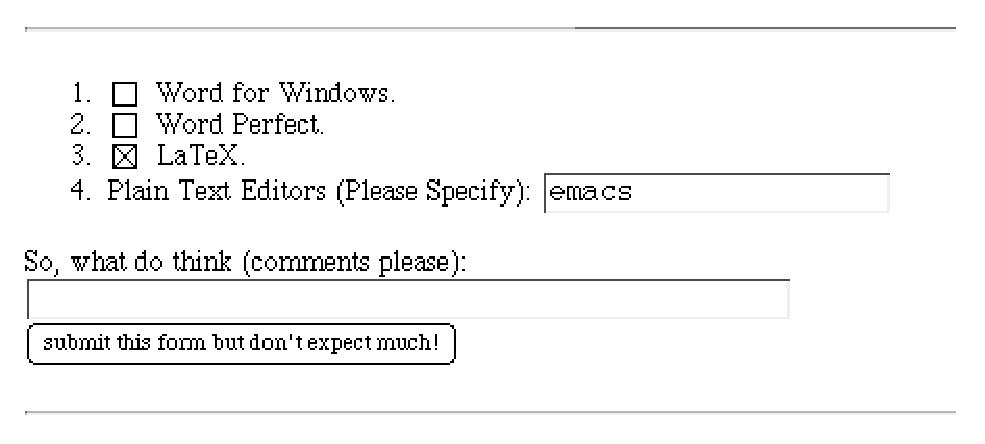
\includegraphics{psfiles/eform.ps}}}
    \end{center}
  \caption{An electronic form.
  In the online version the form would be active.}
  \label{eform}
\end{figure}
\end{latexonly}



\index{rawhtml@\Lc{rawhtml}}%
\paragraph*{\Lc{rawhtml}...\Lc{endrawhtml}\label{endrawhtml}}
\cbversion{97.1}\begin{changebar}
This is an alternative way to specify a chunk of raw \texttt{HTML} code,
using the old \AmS-style of delimiting environments.
Use of this style is discouraged; 
the \env{rawhtml} \htmlref{environment}{rawhtml} is preferred.%
\end{changebar}%

\index{comment@\env{comment} environment}%
\index{environment!comment@\env{comment}}%
\paragraph*{\Lc{begin\char123comment\char125}\label{comment}}
\cbversion{97.1}\begin{changebar}
This environment is simple for the convenience of ``commenting-out''
large sections of source code.
The contents of this environment is completely ignored,
both in the \LaTeX{} and \texttt{HTML} versions.
Such an environment is already used in \AmS-\LaTeX,
and perhaps with other packages.
It is defined here for its general utility.

\noindent
To insert \texttt{SGML}-style comments into the \texttt{HTML} files,
use the \env{rawhtml} environment as follows.
%begin{latexonly}
\begin{small}
%end{latexonly}
\begin{verbatim}
\begin{rawhtml}
<!--  this text is treated as a comment
      perhaps extending over several lines 
-->
\end{rawhtml}
\end{verbatim}
%begin{latexonly}
\end{small}
%end{latexonly}%
\end{changebar}%

\noindent
Note the \hyperref[page]{warning}{warning on page~}{}{env:warn}
concerning how the environment delimiters should be used in the
\LaTeX{} source code.


\index{latexonly@\Lc{latexonly}}%
\paragraph*{\Lc{comment...\char92endcomment}\label{endcomment}}
\cbversion{97.1}\begin{changebar}
This is an alternative way to specify a chunk of material intended
to be ignored in both the \LaTeX{} and \texttt{HTML} versions,
using the old \AmS-style of delimiting environments.
Use of this style (though convenient for typing) is discouraged,
since it is not as reliable as using the \env{comment} \htmlref{environment}{comment}.
\end{changebar}\html{\\}


\subsection{Arbitrary Tags and Attributes\label{sec:arbtags}}%
%\section{Arbitrary Tags and Attributes\label{sec:arbtags}}%
%
For version 97.1 of \latextohtml\ there is a new command which provides 
an extremely flexible way to include \texttt{HTML} 3.2 tags, along with
any values for the ``attributes'' of that tag, if desired.
\begin{quote}
\Lc{HTML}\verb|[|\Meta{attribs}\verb|]{|\Meta{tag}\verb|}|\label{HTMLtag}\\
\Lc{HTML}\verb|[|\Meta{attribs}\verb|]{|\Meta{tag}\verb|}{|\Meta{contents}\verb|}|
\end{quote}
When the \Meta{tag} also needs a closing tag (e.g \texttt{<I>...</I>})
the \Meta{contents} \emph{must} be given, enclosed in braces.
Both the opening and closing tags then will be placed correctly.


An important aspect of this is that any of the \Meta{tag},
\Meta{attribs} and \Meta{contents} may be given wholly
by expanding a \LaTeX{} macro, or may contain arbitrary macros, 
perhaps including other \Lc{HTML} commands.
\hyperref{The following table}{The contents of Figure~}{}{ex:HTML} 
was constructed using this feature; its \LaTeX{} source follows.

\HTML[50\% 3 noshade center]{HR}

\begin{htmlonly}
\begin{figure}
\begin{makeimage}
\end{makeimage}
\newcommand{\myalign}{center}
\newcommand{\mylist}{UL}
\newcommand{\myitem}[2]{\HTML[disc]{LI}{\simpletest{#1}{#2}}}
\newcommand{\simpletest}[2]{%
 \HTML{#1}{ a simple test of ``#2'',} using \HTML{CODE}{<#1>} .}
\newcommand{\tableopts}{10,border=5}

\newcommand{\tablelist}[4][\myalign]{\HTML[#1]{DIV}{
\HTML[\tableopts]{TABLE}{
\HTML[bottom]{CAPTION}{
#3
}\HTML{TR}{\HTML{TD}{
\HTML{#2}{
#4
}}}
}}\HTML[all]{BR}}

\tablelist[\myalign]{\mylist}{%
\textbf{A listing of the different text styles available in HTML 3.2}}{%
\myitem{B}{bold-face}
\myitem{I}{italics}
\myitem{TT}{teletype-text}
\myitem{U}{underlining}
\HTML[circle]{LI}{\simpletest{STRIKE}{strikeout}}
\myitem{EM}{emphasis style}
\myitem{STRONG}{strong style}
\myitem{CODE}{code style}
\myitem{CITE}{citation style}
\myitem{DFN}{definition style}
\HTML[square]{LI}{\simpletest{SAMP}{sample style}}
\HTML[square]{LI}{\simpletest{KBD}{keyboard style}}
\myitem{VAR}{variable style}}
%
 \caption{Example use of macros for raw \texttt{HTML} code.}
 \label{ex:HTML}
\end{figure}
\end{htmlonly}
%
\begin{latexonly}
\begin{figure}[ht]
\begin{center}
  \fbox{\scalebox{.7}{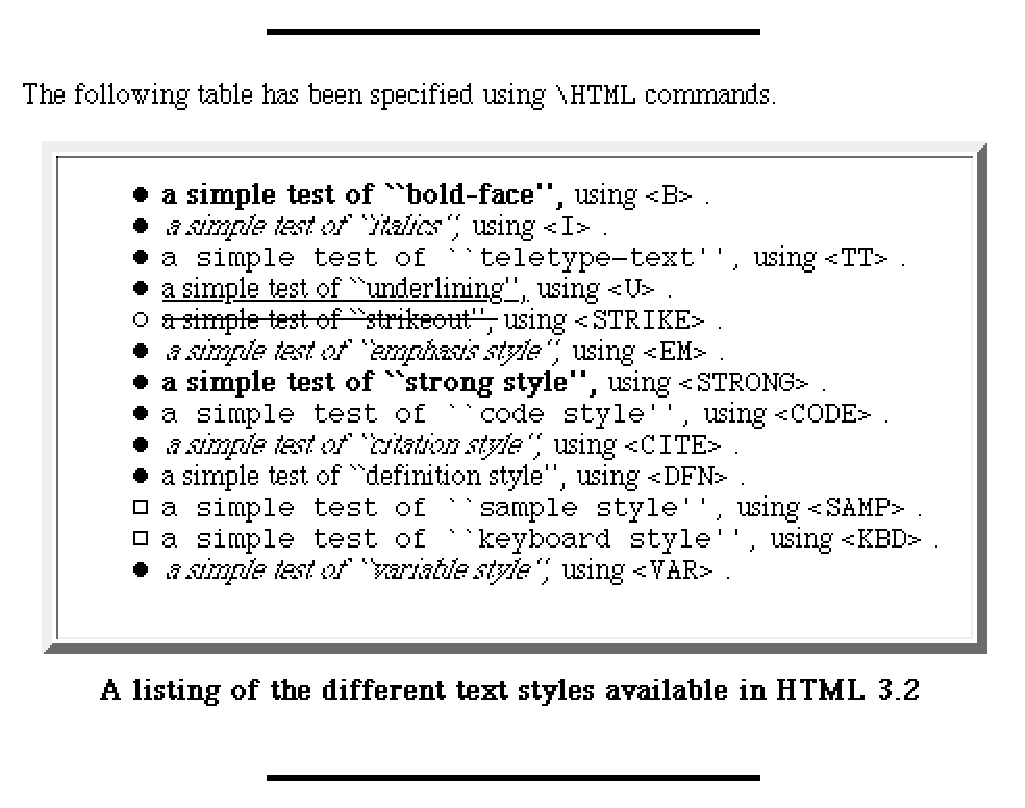
\includegraphics{psfiles/HTMLtab.ps}}}
 \caption{Example use of macros for raw \texttt{HTML} code.}
 \label{ex:HTML}
\end{center}
\end{figure}
\end{latexonly}

\HTML[50\% 3 noshade center]{HR}

%begin{latexonly}
\begin{small}
%end{latexonly}
\begin{verbatim}
\newcommand{\myalign}{center}
\newcommand{\mylist}{UL}
\newcommand{\myitem}[2]{\HTML[disc]{LI}{\simpletest{#1}{#2}}}
\newcommand{\simpletest}[2]{%
 \HTML{#1}{ a simple test of ``#2'',} using \HTML{CODE}{<#1>} .}
\newcommand{\tableopts}{10,border=5}

\newcommand{\tablelist}[4][left]{\HTML[#1]{DIV}{
\HTML[\tableopts]{TABLE}{
\HTML[bottom]{CAPTION}{
#3
}\HTML{TR}{\HTML{TD}{
\HTML{#2}{
#4
}}}
}}\HTML[all]{BR}}

\tablelist[\myalign]{\mylist}{%
\textbf{A listing of the different text styles available in HTML 3.2}}{%
\myitem{B}{bold-face}
\myitem{I}{italics}
\myitem{TT}{teletype-text}
\myitem{U}{underlining}
\HTML[circle]{LI}{\simpletest{STRIKE}{strikeout}}
\myitem{EM}{emphasis style}
\myitem{STRONG}{strong style}
\myitem{CODE}{code style}
\myitem{CITE}{citation style}
\myitem{DFN}{definition style}
\HTML[square]{LI}{\simpletest{SAMP}{sample style}}
\HTML[square]{LI}{\simpletest{KBD}{keyboard style}}
\myitem{VAR}{variable style}}
\end{verbatim}
%begin{latexonly}
\end{small}
%end{latexonly}

\HTML[50\% 3 noshade center]{HR}

\noindent
The above code demonstrates many aspects of the way \Lc{HTML}
commands can be used.
%
\begin{htmllist}\htmlitemmark{GreenBall}
\item [nesting: ] 
\Lc{HTML} commands can be nested to arbitrary depth.
%
\item [macros: ] 
Macros can be used to specify all or part of each argument.
%
\item [within macros: ] 
\Lc{HTML} commands work correctly within the expansions of other macros.
%
\item [attribute values: ]
Information within \Meta{attribs} can be specified in a very
loose way, as a comma-separated list of key/value pairs
or as single values. \\
Not even the commas are necessary: space(s), \Meta{tab}s 
or newlines are equally effective.
Indeed the horizontal rules preceding and following the table were 
specified by:
\begin{quote}
\begin{verbatim}
\HTML[50\% 3 noshade center]{HR}
\end{verbatim}
\end{quote}
%
\item [attribute names: ]
Usually it is \emph{not necessary} to know the names of the
attributes to the tags that are to be used. It is sufficient
just to give the values; these will be matched to the
appropriate attribute, according to the type of data required.
(If names are given, these are case-insensitive.)
%
\item [newlines: ] 
Although \LaTeX{} ignores linebreaks within the source code,
this is not so with \latextohtml. 
The strange spreading-out of the definition of the
\Lc{tablelist} command above was done with the purpose
solely of making the code in the resulting \texttt{HTML} files 
more easily readable, to a human.
(As most browsers ignore those newlines anyway, 
more compact code would have rendered the same on-screen.)
\end{htmllist}

\medskip\noindent
Some further aspects of the use of this \Lc{HTML}
command are not apparent from the above example. 

\begin{htmllist}\htmlitemmark{RedBall}
%
\item [invalid \Meta{tag}\,: ]
If a \Meta{tag} is specified that is not part of the 
\texttt{HTML} 3.2 specifications, then it and its attributes are 
not placed into the \texttt{HTML} document created by \latextohtml.
Any \Meta{contents} \emph{is} included as ordinary data; 
i.e. as text in paragraphs, etc.

\item [required attributes: ] 
Some tags have attributes which are required to have values,
if that tag is to be included in an \texttt{HTML} document.
Using the \Lc{HTML} command, if any such attribute
is not given an appropriate value then the tag is ignored.
Any \Meta{contents} are included in the document, 
as ordinary character data.

\item [valid HTML\,: ] 
Currently there is \emph{no} checking that the \Meta{contents}
of a \Meta{tag} contains only data (perhaps including other tags)
allowed by the DTD for \texttt{HTML} 3.2.
\begin{quote}
\textit{The requirement to produce valid \texttt{\upshape HTML} 
currently rests with the user.}
\end{quote}
This issue will be addressed in forthcoming revisions of \latextohtml.

\item [extra attributes and values: ]
The list of attributes for a \Meta{tag} can include
key-value pairs whose keys do not match any valid
attribute for the \Meta{tag}.
Such key-value pairs are simply ignored.
Similarly extra data values are ignored, 
as are values that do not match the
requirements for any valid attribute.

\item [attributes with similar data-types: ]
Several attributes to a \Meta{tag} may use values having 
the same or similar data-types. First any key-value pairs
are processed. Remaining values are allocated 
to those attributes which do not already have a value.
An ordering of the attributes is used, based on a perceived likelihood 
of each attribute being required to be changed from its default setting.

\end{htmllist}


\subsection{Conditional Text\label{sec:latexonly}}%
%\section{Conditional Text\label{sec:latexonly}}%
\tableofchildlinks*
\index{latexonly@\env{latexonly} environment}%
\index{htmlonly@\env{htmlonly} environment}%
\index{environment!htmlonly@\env{htmlonly}}%
\index{environment!latexonly@\env{latexonly}}%
\index{conditional text!scoped variant}\html{\\}%
\paragraph*{\Lc{begin\char123latexonly\char125} and 
\Lc{begin\char123htmlonly\char125}\label{latexonly}\label{htmlonly}}
Conditional text can be specified
using the environments \env{latexonly} and \env{htmlonly}. 
These allow writing parts of a document which are intended 
only for electronic delivery or only for paper-based delivery.

This would be useful for example in adding a long description of a
multi-media resource in the paper version of a document. 
Such a description would be redundant in the electronic version, 
as the user can have direct access to this resource. 

\medskip\goodbreak\noindent
Here is an example of the use of the \env{latexonly} environment,
used \hyperref[page]{earlier in}{on page~}{ of}{eform} this manual:
%begin{latexonly}
\begin{small}\indent
%end{latexonly}
\Lc{begin}\verb|{latexonly}|
\latex{\vskip-\baselineskip\vskip-\baselineskip}
\begin{verbatim}
\begin{figure}
    \begin{center}
    \fbox{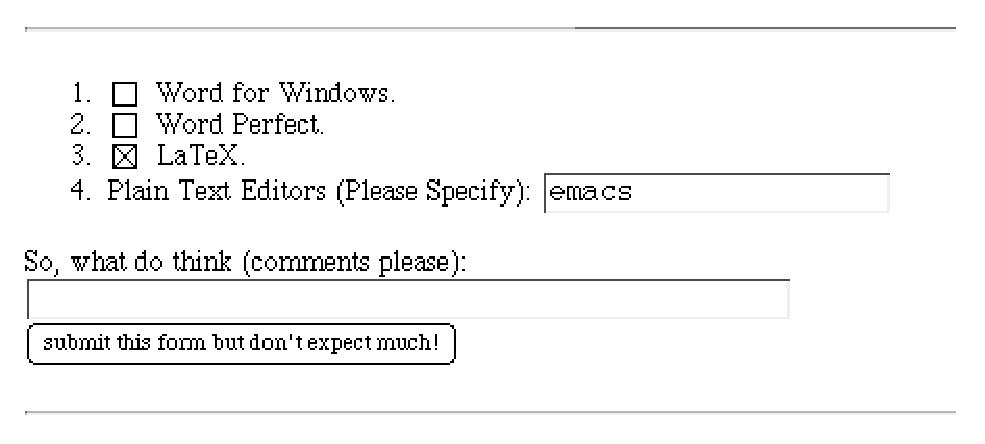
\includegraphics[width=4in]{psfiles/eform.ps}}
    \end{center}
    \caption{An electronic form. Of course in the online version of this
     document the form above would be active.}
\end{figure}
\end{verbatim}
\latex{\nobreak\vskip-\baselineskip\nobreak\indent\indent}%
\Lc{end}\verb|{latexonly}|
%begin{latexonly}
\end{small}\goodbreak\medskip
%end{latexonly}

\noindent
Note the \hyperref[page]{warning}{warning at the bottom of page~}{}{env:warn}
concerning how the environment delimiters should be used in the
\LaTeX{} source code.


\index{htmlonly@\Lc{htmlonly}}%
\paragraph*{\Lc{htmlonly...\char92endhtmlonly}\label{endhtmlonly}}
\cbversion{97.1}\begin{changebar}
This is an alternative way to specify a chunk of material intended
for the \texttt{HTML} version only,
using the old \AmS-style of delimiting environments.
Use of this style is discouraged; 
the \env{htmlonly} \htmlref{environment}{htmlonly} is preferred.%
\end{changebar}%


\index{latexonly@\Lc{latexonly}}%
\paragraph*{\Lc{latexonly...\char92endlatexonly}\label{endlatexonly}}
\cbversion{97.1}\begin{changebar}
This is an alternative way to specify a chunk of material intended
for the \LaTeX{} typeset version only,
using the old \AmS-style of delimiting environments.
Use of this style is discouraged; 
the \env{latexonly} \htmlref{environment}{latexonly} or the unscoped 
\htmlref{\texttt{\%begin\char123latexonly\char125}}{unlatexonly} 
construction are preferred.%
\end{changebar}%

\smallskip\noindent
Note the \hyperref[page]{warning}{warning at the bottom of page~}{}{env:warn}
concerning how the environment delimiters should be used in the
\LaTeX{} source code.


\index{conditional text!shorthand notation}%
\index{latex@\Lc{latex}}%
\index{html@\Lc{html}}%
\index{latexhtml@\Lc{latexhtml}}\html{\\}%
\paragraph*{\Lc{latex}, \Lc{html} and \Lc{latexhtml}\label{latexhtml}}
\cbversion{96.1}\begin{changebar}
There are also shorthand notations to accomplish the same thing 
as in the \env{latexonly} \htmlref{environment}{latexonly} and \env{htmlonly} 
\htmlref{environment}{htmlonly}, but with less typing.
\begin{itemize}
\item 
The \Lc{latex}\verb|{...}| command causes everything within the braces 
to be processed by \LaTeX, but ignored by \latextohtml.
\item  
Conversely, the \Lc{html}\verb|{...}| command causes everything within the braces 
to be ignored by \LaTeX{} and processed by \latextohtml.  
\item  
Finally the command \Lc{latexhtml}\verb|{...}{...}| causes everything 
within the first set of braces to be processed exclusively by \LaTeX, 
with the contents of the second set of braces processed solely by \latextohtml.%
\end{itemize}
\textbf{Warning: }
Only small pieces of text work reliably in this way. 
With whole paragraphs or contained sub-environments,
the ``conditional'' environments should be used instead.
\end{changebar}

\index{conditional text!without scope}%
\index{beginlatex@\texttt{\%{}begin\char123latexonly\char125}}%
\index{endlatex@\texttt{\%{}end\char123latexonly\char125}}%
\paragraph*{\texttt{\%begin\char123latexonly\char125}\label{unlatexonly}}
Another variant of the \env{latexonly} environment is available, 
in which everything between 
\verb|%|\verb|begin{latexonly}| and \verb|%|\verb|end{latexonly}| 
is ignored by \latextohtml.  
The difference is that the \env{latexonly} environment 
puts the contents into a group, in which all definitions are local.
There is no such scoping with the \verb|%begin...%end| variant,
since \LaTeX{} sees the initial \texttt{\%}s simply as starting comments.%

\medskip
\index{conditional text!example}\html{\\}\noindent
The following example should clarify what happens:
%begin{latexonly}
\begin{small}
%end{latexonly}
\begin{verbatim}
\newcommand{\A}{The letter A.}
\newcommand{\B}{The letter B.}
\end{verbatim}
\indent\indent\indent\verb|\|\verb|begin{latexonly}|\\
\indent\indent\verb|\renewcommand{\A}{Not the letter A.}|\\
\indent\indent\verb|\|\verb|end{latexonly}|\\
\indent\indent\verb|%|\verb|begin{latexonly}|\\
\indent\indent\verb|\renewcommand{\B}{Not the letter B.}|\\
\indent\indent\verb|%|\verb|end{latexonly}|
\begin{verbatim}
\begin{document}
\A \B
\end{document}
\end{verbatim}
%begin{latexonly}
\end{small}
%end{latexonly}
If you process this with \LaTeX, the result is: 
\quad\quad The letter A. Not the letter B.

\smallskip\noindent
Note the \hyperref[page]{warning}{warning at the bottom of page~}{}{env:warn}
concerning how the environment delimiters should be used in the
\LaTeX{} source code.

\medskip\index{conditional text!avoid using counters}\html{\\}\noindent
\textbf{Warning: }% 
Be careful when using \LaTeX{}  commands which alter the values of counters 
(e.g. numbered figures or equations) in conditional text, because this may 
cause the counter values in the electronic version to lose synchronisation 
with the values of the corresponding counters in the \LaTeX{} version.


\htmlrule[width=300]
\index{imagesonly@\env{imagesonly} environment}%
\index{environment!imagesonly@\env{imagesonly}}%
\paragraph*{\Lc{begin\char123imagesonly\char125}\label{imagesonly}}
\cbversion{97.1}\begin{changebar}
This environment is used to put \LaTeX{} code into the \fn{images.tex} file,
to be used when generating images. Typically this is used to add commands to
the preamble of \fn{images.tex}, such as setting the text or background color.
However code can be added at any other point as well; 
e.g. to change the background color of all images after a certain point in the document. 
\end{changebar}%

\smallskip\noindent
Note the \hyperref[page]{warning}{warning at the bottom of page~}{}{env:warn}
concerning how the environment delimiters should be used in the
\LaTeX{} source code.


\index{makeimage@\env{makeimage} environment}%
\index{environment!makeimage@\env{makeimage}}%
\paragraph*{\Lc{begin\char123makeimage\char125}\label{makeimage}}
\cbversion{97.1}\begin{changebar}
This is a special environment which forces an image to be made of its contents.
That is, one gets effectively a snapshot of a portion of a page
that has been typeset using \LaTeX. 
Within the normal \LaTeX{} typeset version of the document, this environment 
is completely transparent, adding its contents to the page as usual.

\index{makeimage@\env{makeimage} environment!inside@inside a \env{figure}}\html{\\}%
One further important use of the \env{makeimage} environment is as follows.
If a \env{makeimage} environment occurs as a sub-environment within 
a \env{figure} environment, then an image will \emph{not} be made of the
\env{figure}'s contents. Instead, the contents are treated as normal text,
each part being handled as if there were no \env{figure} at all,
except that everything is placed within a single cell of a
\HTMLtag{TABLE}...\HTMLtag{/TABLE} construction in \HTMLiii. 
The contents of any \Lc{caption}
commands are placed between \HTMLtag{CAPTION}...\HTMLtag{/CAPTION} tags 
for the \HTMLtag{TABLE}.

\index{makeimage@\env{makeimage} environment!empty sub-environment}\html{\\}%
Normally an image of the entire contents of the \env{figure} would be
placed within the single cell of the \HTMLtag{TABLE}.
Now images are made of any subparts of those \env{figure}'s contents 
that really need it, in particular the \env{makeimage} sub-environments.
An empty \env{makeimage} sub-environment does not generate an image of itself,
yet still it inhibits an image being made of the whole \env{figure}.
These comments apply also to \env{table} environments.
\end{changebar}\html{\\}




\subsection{Symbolic References shown as Hyperized Text\label{hyperized}%
%\section{Symbolic References shown as Hyperized Text\label{hyperized}%
\index{references@references\protect\label{IIIrefs}}}%
\tableofchildlinks*
\index{cross-references!|see{\htmlref{references}{IIIrefs}}}%
\index{references!symbolic\label{IIIsymref}}\index{symbolic labels|(}%
\index{references!numeric}%
\index{references!iconic}\html{\\}\noindent
In printed documents cross-references are shown 
through a \emph{numeric or symbolic indirection} 
e.g. ``see Figure 1'' (numeric indirection), 
or ``see section `Changes'~'' (symbolic indirection).  
\latextohtml{} can mirror this mechanism using the same numeric 
or symbolic references,
or when these are not appropriate by using iconic references.

\index{references!without indirection}%
\index{references!highlighted text}\html{\\}%
In a hypertext document however, cross-references can be shown 
without any indirection, just by highlighting a relevant piece of text. 
This can make a document more readable as it removes unnecessary
information. 

\index{hyperref@\Lc{hyperref}}%
\paragraph*{\Lc{hyperref}\label{hyperref}}
A single new \LaTeX{} command \Lc{hyperref} can be used for
specifying how a cross-reference should appear, 
both in the printed document and in the hypertext version.
For example, assuming that the label \verb|{sec:cond}|\label{sec:cond} 
is defined somewhere within a document, 
the command \Lc{hyperref}, taking 4 arguments,
can be used in that document as follows:
\index{hyperref@\Lc{hyperref}}%
\index{conditional text}%
%begin{latexonly}
\begin{small}
%end{latexonly}
\begin{verbatim}
\emph{Is the concept of
\hyperref
               % This will be highlighted in the hypertext version
{conditional text}			% argument #1
               % This will be shown in the printed version 
               % followed by a numeric reference ...      
{conditional text (see Section }  	% argument #2
               % ... followed by this text
{ for more information)} 		% argument #3
               % This is the common label 
{sec:cond}				% argument #4
a good idea? }
\end{verbatim}
%begin{latexonly}
\end{small}
%end{latexonly}

\noindent
Here is how it will be shown:
\begin{quote}
\emph{Is the concept of
\hyperref
% This will be highlighted in the hypertext version
{conditional text}
% This will be shown in the printed version  
% followed by a numeric reference ...      
{conditional text (see Section }  
% ... followed by this text
{ for more information)} 
% This the common label 
{sec:cond}
a good idea? }
\end{quote}

\begin{htmlonly}
In the printed version what would appear is:
\begin{quote}
\emph{Is the concept of conditional text (see Section 4.2 for more information) 
a good idea?}
\end{quote}
\end{htmlonly}

\begin{latexonly}%
In the hypertext version what would appear is:
\begin{quote}
\emph{Is the concept of \underline{conditional text} a good idea?}
\end{quote}
(Of course \underline{conditional text} would be an active hypertext link.)
\end{latexonly}

\bigskip\htmlrule[50\% center]
\cbversion{97.1}\begin{changebar}%
\noindent
An extended syntax for \Lc{hyperref} uses an optional argument, 
which determines what information is to be placed in the \LaTeX{} version
of the document. The value of this optional argument can also affect 
the number of required arguments. 
These forms are recognised:

%begin{latexonly}
\begin{small}
%end{latexonly}
\begin{quote}\label{hypernoref}
\Lc{hyperref}\verb|[ref]{|\Meta{HTML-text}\verb|}{|\Meta{LaTeX-text}%
\verb|}{|\Meta{post-LaTeX}\verb|}{|\Meta{label}\verb|}|\\
\Lc{hyperref}\verb|{|\Meta{HTML-text}\verb|}{|\Meta{LaTeX-text}%
\verb|}{|\Meta{post-LaTeX}\verb|}{|\Meta{label}\verb|}|\medskip

\Lc{hyperref}\verb|[pageref]{|\Meta{HTML-text}\verb|}{|\Meta{LaTeX-text}%
\verb|}{|\Meta{post-LaTeX}\verb|}{|\Meta{label}\verb|}|\\
\Lc{hyperref}\verb|[page]{|\Meta{HTML-text}\verb|}{|\Meta{LaTeX-text}%
\verb|}{|\Meta{post-LaTeX}\verb|}{|\Meta{label}\verb|}|\medskip

\Lc{hyperref}\verb|[noref]{|\Meta{HTML-text}\verb|}{|\Meta{LaTeX-text}%
\verb|}{|\Meta{label}\verb|}|\\
\Lc{hyperref}\verb|[no]{|\Meta{HTML-text}\verb|}{|\Meta{LaTeX-text}%
\verb|}{|\Meta{label}\verb|}|
\end{quote}
%begin{latexonly}
\end{small}
%end{latexonly}

\noindent
The first two are the defaults, where \LaTeX{} 
uses \Lc{ref}\verb|{|\Meta{label}\verb|}|.
With the next two \LaTeX{} uses \Lc{pageref}\verb|{|\Meta{label}\verb|}|,
while with the final two \LaTeX{} completely ignores the \Meta{label},
setting just the \Meta{LaTeX-text}.
\end{changebar}

\medskip
\index{hyperref@\Lc{hyperref}!pageref@\Lc{pageref} example}%
\html{\\}\noindent
For creating hyperlinks to other documents
using symbolic reference \Meta{label}s, 
see also the \Lc{externalref} 
\hyperref[page]{command}{command, described on page~}{}{externref}.

\medskip\noindent
The preceding paragraph is an example of the use of the \Lc{hyperref[page]} option.
Its source code is:
%begin{latexonly}
\begin{small}
%end{latexonly}
\begin{verbatim}
For creating hyperlinks to other documents
using symbolic reference \Meta{label}s, 
see also the \Lc{externalref} 
\hyperref[page]{command}{command, described on page~}{}{externref}.
\end{verbatim}
%begin{latexonly}
\end{small}
%end{latexonly}
\begin{htmlonly}
which appears in the \LaTeX{} typeset version as:
\begin{quote}
For creating hyperlinks to other documents
using symbolic reference \Meta{label}s, see also the
\Lc{externalref} command, described on page~31.
\end{quote}
\end{htmlonly}
\begin{latexonly}
which appears in the \texttt{HTML} version as:
\begin{quote}
For creating hyperlinks to other documents, using symbolic reference \Meta{label}s, 
see also the \Lc{externalref} \underline{command}.
\end{quote}
with the \underline{command} being an active hyperlink.
\end{latexonly}
\smallskip\noindent
In fact both \Lc{hyperref} and the \Lc{htmlref} command, to be described next,
permit textual hyperlinks based on symbolic \Meta{label}s from external files.


\index{htmlref@\Lc{htmlref}}%
\index{html.sty@\texttt{html.sty} style-file}
\paragraph*{\Lc{htmlref}\label{htmlref}}
Another command also defined in \fn{html.sty} is \Lc{htmlref} 
which has the same effect as \Lc{hyperref}
during the conversion to \texttt{HTML}.
It takes two arguments, some text and a label. 
In the \texttt{HTML} version the
text will be ``hyperized'', pointing to the label. 
In the paper version the text will be shown as it is 
and the label will be ignored; e.g.
%
\index{htmlref@\Lc{htmlref}!easy to make links}%
%begin{latexonly}
\begin{small}
%end{latexonly}
\begin{verbatim}
With \verb|\htmlref| \htmlref{it's easy to make links}{fig:example}.
\end{verbatim}
%begin{latexonly}
\end{small}
%end{latexonly}
which produces:
\begin{quote}
With \Lc{htmlref} \htmlref{it's easy to make links}{fig:example}.
\end{quote}
\begin{htmlonly}
In the \LaTeX{} typeset version it will appear simply as:
\begin{quote}
With \Lc{htmlref} it's easy to make links.
\end{quote}
\end{htmlonly}
\begin{latexonly}
In the \texttt{HTML} version it is shown as:
\begin{quote}
With \Lc{htmlref} \underline{it's easy to make links}.
\end{quote}
\end{latexonly}
\html{\\}
\goodbreak

\subsection{Hypertext Links in Bibliographic References (Citations)}%
%\section{Hypertext Links in Bibliographic References (Citations)}%
\tableofchildlinks*
\index{references!bibliographic}\index{bibliography|(}%
\index{bibliography!bibliographic database}%
\index{bibliography!using .bib@using \texttt{.bib} file}\html{\\}%
If a report or a book that is cited (using the \Lc{cite} command) 
is available (or there is information about it) on the World-Wide
Web, then it is possible to add the appropriate hypertext links
in your bibliographic database (the \texttt{.bib}) file. 

\bigskip
\index{bibliography!example using URLs}%
\index{bibliography!string commands@\texttt{\char64 string} commands}%
\index{LaTeX blue book@\LaTeX{} blue book}\html{\\}%
\noindent
Here is an example of a bibliographic entry for the original
\LaTeX{} \cite{lamp:latex} blue book:\nobreak
%begin{latexonly}
\begin{small}
%end{latexonly}
\begin{verbatim}
@string{curiaURL="\htmladdnormallink
{http://curia.ucc.ie/info/TeX/menu.html}
{http://curia.ucc.ie/info/TeX/menu.html}"}

@string{fernURL="\htmladdnormallink
{http://es-sun2.fernuni-hagen.de/info2html?(latex.info)Top}
{http://es-sun2.fernuni-hagen.de/info2html?(latex.info)Top}"}

@book{lamp:latex,
title = "LaTeX User's Guide \& Reference Manual, 2nd edition",
year = 1994 ,
author = "Leslie Lamport",
Publisher = "Addison--Wesley Publishing Company, Inc.",
note = "Online information on {\TeX} and {\LaTeX} is available at "
 # curiaURL # " and " # fernURL }
\end{verbatim}
%begin{latexonly}
\end{small}
%end{latexonly}
See the \htmlref{bibliography}{biblio} for how this will appear.\html{\\}
No other modifications are required; \LaTeX{} and Bib\TeX{} should work as normal.
%
\index{bibliography!string commands@\texttt{\char64string} commands}%
\cbversion{96.1f}\begin{changebar}
Note that it would be sensible to put the \texttt{@string} commands
into a separate file, \fn{urls.bib} say, 
loaded with the main file via\html{\\} \verb|\bibliography{urls,...}|.%
\end{changebar}

\smallskip\index{citations!Harvard style}%
\index{bibliography!Harvard style}\label{harvard}\html{\\}%
\noindent
For those who use the Harvard style for references
\htmladdnormallinkfoot{there exists a special conversion add-on package}%
{http://www.arch.su.edu.au/\~{}peterw/latex/harvard/}.

\index{citations!natbib@\env{natbib} package}%
\index{bibliography!natbib@\env{natbib} package}%
\index{citations!Harvard style!handled@handled by \env{natbib}}%
\cbversion{96.1g}\begin{changebar}
The \env{natbib} package, written for \LaTeX{} by \PatrickDaly,
provides even more flexibility in the way a reference may be cited. 
All the features of \htmlref{this package}{natbib} are implemented 
for \latextohtml{} via the \fn{natbib.perl} file.
(Indeed there is even a mode whereby \env{natbib} handles
the Harvard style of citation. 
This requires loading also the \env{nharvard} \htmlref{package}{nharvard}.)

\medskip
\noindent\textbf{Thanks...} to \Wilck\ for the bulk of the work 
in producing this extension, and to \RossMoore\ for 
necessary adjustments to allow it to work correctly with the 
\htmlref{document segmentation strategy}{Segmentation}.
\end{changebar}


\index{hypercite@\Lc{hypercite}}%
\paragraph*{\Lc{hypercite}\label{hypercite}}
\cbversion{97.1}\begin{changebar}
Analogous to \Lc{hyperref} is the \Lc{hypercite} command,
which allows a free-form textual hyperlink to the bibliography,
whereas the \LaTeX{} typeset version contains the usual citation code.
The allowed syntax is as follows.
%begin{latexonly}
\begin{small}
%end{latexonly}
\begin{quote}
\Lc{hypercite}\verb|[int]{|\Meta{HTML-text}\verb|}{|\Meta{LaTeX-text}%
\verb|}{|\Meta{opt-LaTeX}\verb|}{|\Meta{label}\verb|}|\\
\Lc{hypercite}\verb|[cite]{|\Meta{HTML-text}\verb|}{|\Meta{LaTeX-text}%
\verb|}{|\Meta{opt-LaTeX}\verb|}{|\Meta{label}\verb|}|\\
\Lc{hypercite}\Meta{HTML-text}\verb|}{|\Meta{LaTeX-text}%
\verb|}{|\Meta{opt-LaTeX}\verb|}{|\Meta{label}\verb|}|\medskip

\Lc{hypercite}\verb|[nocite]{|\Meta{HTML-text}\verb|}{|\Meta{LaTeX-text}%
\verb|}{|\Meta{label}\verb|}|\\
\Lc{hypercite}\verb|[no]{|\Meta{HTML-text}\verb|}{|\Meta{LaTeX-text}%
\verb|}{|\Meta{label}\verb|}|\\
\Lc{hypercite}\verb|[ext]{|\Meta{HTML-text}\verb|}{|\Meta{LaTeX-text}%
\verb|}{|\Meta{label}\verb|}|
\end{quote}
%begin{latexonly}
\end{small}
%end{latexonly}
The first three forms are equivalent; 
\LaTeX{} uses \Lc{cite}\verb|[|\Meta{opt-LaTeX}\verb|]|\Meta{label}\,,
after placing the \Meta{LaTeX-text}.
Note that \verb|{|\Meta{opt-LaTeX}\verb|}| \emph{must} be specified, 
even if empty `\verb|{}|'.

Similarly the latter three forms are equivalent, 
with \LaTeX{} using \Lc{nocite}\verb|{|\Meta{label}\verb|}|\,, 
to force the particular reference to appear on the bibliography page, 
even though no explicit marker is placed at this point.
(Thus there is no need for an optional  \Meta{opt-LaTeX} argument.)\html{\\}
Within the \texttt{HTML} version a hyperlink is produced when the \Meta{HTML-text} 
is not empty. External label files are also searched, 
in order to match the symbolic \Meta{label}, see also 
\hyperref[page]{\Lc{externalcite}}{\Lc{externalcite} on page~}{}{externcite}.

\smallskip\noindent\label{hyperciteXmpl}%
\index{hypercite@\Lc{hypercite}!example}%
\index{htmlcite@\Lc{htmlcite}!example}\html{\\}\noindent
\htmlref{Earlier}{hypcites} in this manual the following source code was used:
%begin{latexonly}
\begin{small}
%end{latexonly}
\begin{verbatim}
commands described in the \LaTeX{} \htmlcite{blue book}{lamp:latex}, 
...
as well as many other \LaTeX{} constructions, such as are described in 
the \LaTeX{} \hypercite{\emph{Companion}}{\emph{Companion}}{}{goossens:latex} 
and \LaTeX{} \hypercite{\emph{Graphics Companion} (e.g. \Xy-pic)}%
{\emph{Graphics Companion}}{\Xy-pic}{goossens:latexGraphics};
\end{verbatim}
%begin{latexonly}
\end{small}
%end{latexonly}
which produces:
\begin{quote}
commands described in the \LaTeX{} \htmlcite{blue book}{lamp:latex}, 
\\~~...\\
as well as many other \LaTeX{} constructions, such as are described in 
the \LaTeX{} \hypercite{\emph{Companion}}{\emph{Companion}}{}{goossens:latex} 
and \LaTeX{} \hypercite{\emph{Graphics Companion} (e.g. \Xy-pic)}%
{\emph{Graphics Companion}}{\Xy-pic}{goossens:latexGraphics};
\end{quote}
\begin{latexonly}
whereas in the \texttt{HTML} version one sees:
\begin{quote}
commands described in the \LaTeX{} \underline{blue book}, 
\\~~...\\
as well as many other \LaTeX{} constructions, 
such as are described in the \LaTeX{} \underline{\emph{Companion}} 
and  \LaTeX{} \underline{\emph{Graphics Companion} (e.g. \Xy-pic)};
\end{quote}
\end{latexonly}
%
\begin{htmlonly}
whereas in the \LaTeX{} typeset version one sees:
\begin{quote}
commands described in the \LaTeX{} blue book,\\
~~...\\
as well as many other \LaTeX{} constructions, such as are described in the \LaTeX{} 
\textit{Companion}[2] and \LaTeX{} \textit{Graphics Companion}[3, \Xy-pic];
\end{quote}
\end{htmlonly}
\end{changebar}%


\index{htmlcite@\Lc{htmlcite}}%
\paragraph*{\Lc{htmlcite}\label{htmlcite}}
\cbversion{97.1}\begin{changebar}
Analogous to \Lc{htmlref} is the \Lc{htmlcite} command,
which creates a textual hyperlink to a place on the document's bibliography page, 
but without displaying any reference marker in the \LaTeX{} typeset version.
(See \htmlref{above}{hyperciteXmpl} for an example.)%

The \Lc{externalcite} 
\hyperref[page]{command}{command, described on page~}{, }{externcite}
provides a similar facility when the bibliography page is ``external'';
that is, not part of the current document.%
\end{changebar}

\index{bibliography|)}



\subsection{Symbolic References between Living Documents\label{external_cross}}%
%\section{Symbolic References between Living Documents\label{external_cross}}%
\tableofchildlinks*
\index{external references|(}
\index{references!to external documents}%
\index{references!symbolic}%
\index{symbolic labels!see also@\emph{see also} 
 \htmlref{references, symbolic}{IIIsymref}}%
\index{labels!symbolic}%
%
\cbversion{96.1}\begin{changebar}
The method of the previous section to generated
symbolic \htmlref{hyperized}{hyperized} links can
easily be extended to \emph{external} documents processed by \latextohtml.  
When \latextohtml{} processes a document, it generates a \Perl{} file 
named \Meta{prefix}\fn{labels.pl}
which contains a list of all the symbolic labels that were defined, 
along with their locations.  
The \htmlref{\Meta{prefix}}{prefix} is empty unless otherwise specified, 
to allow different document segments to share the same directory.  
\end{changebar}

\index{externallabels@\Lc{externallabels}}%
\index{externalref@\Lc{externalref}}%
\paragraph*{\Lc{externallabels}\label{externlabels}}
\cbversion{96.1}\begin{changebar}
Links to an external document are then possible once a connection 
is established to that document's \fn{labels.pl} file.  
This connection is established by the \Lc{externallabels} command:%
\end{changebar}%
%
\begin{quote}
%begin{latexonly}
\begin{small}
%end{latexonly}
\Lc{externallabels}\verb|{|\Meta{URL to directory of external document}\verb|}|\\
\verb|               {|\Meta{local copy of external document labels.pl file}\verb|}|
%begin{latexonly}
\end{small}
%end{latexonly}
\end{quote}
%
\index{labels!external}\html{\\}%
The first argument to \Lc{externallabels} should be a URL to 
the directory containing the external document.  
The second argument
should be the full path-name to the \fn{labels.pl} file belonging
to the external document.  Note that for \emph{remote} external documents
it is necessary to copy the \fn{labels.pl} file locally so that it
can be read when processing a local document that uses it.
The command \Lc{externallabels} can be used once for each external
document in order to import the \textit{external labels}\label{externallabels}
into the current document.
A warning is given if \fn{labels.pl} cannot be found.

\begin{changebar}%
If a symbolic reference made in either of the commands described
\hyperref{on the previous page}{in Section~}{}{hyperized} is not 
defined within the document itself,
\latextohtml{} will look for that reference in one of the external
files\footnote{Care must be taken to ensure that critical symbolic
references are unique across related documents.}.
After any modifications in an external document 
(sections added/deleted, segmentation into different physical parts, etc.) 
a new \fn{labels.pl} will be generated.  
If the \Lc{externallabels} command in another 
document contains the correct address to an updated copy of
the \fn{labels.pl} file, then the cross-references will be re-aligned
after running the local document through the translator.

\index{labels!internal}\label{internallabels}\html{\\}%
There is also a mechanism analogous to the
\textit{label--ref} pairs of \LaTeX, which can be used only 
within a single document. 
These labels are called \textit{internal labels},
as opposed to the \htmlref{external labels}{externallabels} defined above.
They are used extensively with the document segmentation strategy
described \hyperref{later}{in Section~}{}{Segmentation}.

Either type of label is defined with a \LaTeX{} \Lc{label} command.  
Labels can be referenced \textit{within} a document using a \Lc{ref} command.
When processed by \LaTeX, each \Lc{ref} command is replaced by the 
section number in which the corresponding \Lc{label} occurred.
When processed by the translator, each \Lc{ref} is replaced by 
a hypertext link to the place where the corresponding \Lc{label} occurred.%
\end{changebar}%
 

\index{references!to external documents}%
\index{externalref@\Lc{externalref}}%
\paragraph*{\Lc{externalref}\label{externref}}
\begin{changebar}%
This mechanism can be extended to external documents:
\begin{quote}
%begin{latexonly}
\begin{small}
%end{latexonly}
\Lc{externalref}\verb|{|\Meta{symbolic label in remote document}\verb|}|
%begin{latexonly}
\end{small}
%end{latexonly}
\end{quote}
The argument to \Lc{externalref} may be any symbolic label defined 
in the \fn{labels.pl} file of any of the external documents.
Such references to external symbolic labels are then translated
into hyper-links pointing to the external document.%
\end{changebar}%


\index{citations!within external bibliographies}%
\index{externalcite@\Lc{externalcite}}%
\paragraph*{\Lc{externalcite}\label{externcite}}
\cbversion{97.1}\begin{changebar}
%
Analogous to \htmlref{\Lc{externalref}}{externref},
the \Lc{externalcite} command is used to create a citation link,
where the bibliography page is not part of the current document.
As with \Lc{externalref} symbolic labels for the bibliography page
must have been loaded using 
\htmlref{\Lc{externallabels}}{externlabels}.

A particularly important use for this is in allowing multiple documents 
to access information in a common bibliographic listing.
For example: all of an author's publications; 
a comprehensive listing of publications in a particular field; 
the (perhaps yearly) output of publications 
from a particular organisation or institution.

\medskip\noindent
\textbf{Thanks...} to \Engberg\ for suggesting this feature.
\end{changebar}

\index{external references|)}


\subsubsection{Cross-Referencing Example\label{crossrefs}}% 
%\subsection{Cross-Referencing Example\label{crossrefs}}% 
To understand this mechanism better consider 
how you would maintain a link to this section  
(of the hypertext version of this document) from one of your documents,
without using labels.
Sure enough you can get the name of the physical file that this section is in. 
This however is quite likely to change, and any links to it would become invalid. 
\index{link validation!done by hand}%
To update your link, the name of the new file must be found 
and your link changed by hand. 
Also there is no general updating mechanism, so the only way to find
out if your document is pointing to the right place is by actually
following the link, then doing a manual update\footnote{%
Link validation can be done automatically but the updating must be done
manually when filenames have changed (assuming no other symbolic label
mechanism is available).}.

\index{link validation!symbolic labels}\html{\\}%
Next consider how it could be done with symbolic labels. 
First you have to import the labels used in this document 
by copying the file \htmladdnormallink{\fn{labels.pl}}
{http://cbl.leeds.ac.uk/nikos/tex2html/doc/manual/labels.pl},
saving it in \path{/tmp/labels.pl} say,
then adding anywhere in your document:
%begin{latexonly}
\begin{small}
%end{latexonly}
\begin{verbatim}
\externallabels{http://cbl.leeds.ac.uk/nikos/tex2html/doc/manual}%
               {/tmp/labels.pl}
\end{verbatim}
%begin{latexonly}
\end{small}
%end{latexonly}
After that you can use the label `\texttt{crossrefs}' defined at the beginning of this 
section\footnote{You either have to guess the role of each label by
looking at the \fn{labels.pl} file or by asking the author!} as follows:
%begin{latexonly}
\begin{small}
%end{latexonly}
\begin{verbatim}
\externalref{crossrefs}
\end{verbatim}
%begin{latexonly}
\end{small}
%end{latexonly}
This will be translated into the appropriate hyper-link to this page.
If there are any changes in this document and you would like to
bring your document up-to date, you have to copy 
\htmladdnormallink{\fn{labels.pl}}%
{http://cbl.leeds.ac.uk/nikos/tex2html/doc/manual/labels.pl} again
and rerun the translator on your document. Of course if I move the 
directory containing the \texttt{HTML} files for this document somewhere else, 
then you would have to make a change in the argument of the 
\Lc{externallabels} command to reflect this. 

\index{references!collaboration required}%
It is obvious that some level of collaboration is required between
authors trying to maintain cross-references between different documents. 
Using symbolic labels makes this a lot easier 
(especially for documents written by the same author).
\index{symbolic labels|)}



\subsection{Miscellaneous commands for \texttt{HTML} effects\label{misceffects}}%
%\section{Miscellaneous commands for \texttt{HTML} effects\label{misceffects}}%
\tableofchildlinks*
\index{html.sty@\texttt{html.sty} style-file}%

\noindent
The \env{html} package, through the \LaTeX{} input file \fn{html.sty},
and its \Perl{} counterpart \fn{html.perl}, implements several 
new commands that are intended entirely for effects within the
produced \texttt{HTML} files. In \LaTeX{} these commands, their arguments,
and any optional arguments are completely ignored.

\index{htmlrule@\Lc{htmlrule}}%
\index{visual separation!using \Lc{htmlrule}}%
\paragraph*{\Lc{htmlrule } and 
 \Lc{htmlrule*}\label{htmlrule}}
One such device provided by \fn{html.sty},
is the \Lc{htmlrule} command. 
This puts a horizontal rule into the \texttt{HTML} file only;
being ignored in the \texttt{.dvi} version. 
It is useful to provide extra visual separation between paragraphs,
without creating a new \texttt{HTML} page, 
such as might warrant extra vertical space within the printed version.

\index{htmlrule!htmlrulestar@\Lc{htmlrule*}}%
\index{htmlrule!variants}%
\index{htmlrule!attributes@attributes to the \HTMLtag{HR} tag}%
\cbversion{97.1}\begin{changebar}
Much variation can be obtained in the horizontal rule that is produced,
using extended forms of the \Lc{htmlrule} command:
\begin{quote}
%begin{latexonly}
\begin{small}
%end{latexonly}
\Lc{htmlrule}\\
\Lc{htmlrule*}\\
\Lc{htmlrule[}\Meta{attribs}\texttt{]}\\
\Lc{htmlrule*[}\Meta{attribs}\texttt{]}
%begin{latexonly}
\end{small}
%end{latexonly}
\end{quote}
Whereas a ``break'' tag \HTMLtag{BR} normally precedes the \HTMLtag{HR} generated
by the \Lc{htmlrule} command, 
this break is omitted when using the \Lc{htmlrule*} variant. 

\htmlrule[center,width=200]

\noindent
Furthermore, the optional argument \Meta{attribs} can be used to specify 
attributes for \emph{both} the \HTMLtag{HR} and \HTMLtag{BR} tags. 
More specifically, \Meta{attribs} should be a list of attribute-names 
and/or key-value pairs \texttt{\Meta{key}=\Meta{value}} separated by spaces or commas. 
This list is parsed to extract those attributes applicable to the \HTMLtag{HR} tag,
and those applicable to the \HTMLtag{BR} (with the unstarred variant).

\medskip\htmlrule[right,width=200,size=5]
\noindent
Using \HTMLiii, this allows variations to be specified for:
\begin{itemize}
\item 
the (vertical) thickness of the horizontal line in pixels: \texttt{SIZE=\Meta{num}};
\item 
the (horizontal) width of the line in pixels or points: \texttt{WIDTH=\Meta{width}};
\item 
alignment: \texttt{WIDTH=\char34...\char34 } 
taking \texttt{left}, \texttt{right} or \texttt{center};
\item 
removal of the shadowed effect \texttt{NOSHADE};
\item 
positioning of the rule with respect to text-flows: 
\texttt{CLEAR=\char34...\char34 } 
taking \texttt{left}, \texttt{all}, \texttt{right} or \texttt{none}. 
\htmlrule[right,width=200,size=5]
\end{itemize}%
Some examples of these effects appear on 
\latex{the \texttt{HTML} version of} this page.%
\end{changebar}%


\index{strikeout@\Lc{strikeout}}%
\paragraph*{\Lc{strikeout\char123}\Meta{text}\texttt{\char125}\label{strikeout}}
\cbversion{97.1}\begin{changebar}
With this command the \Meta{text} is processed as normal in the \texttt{HTML} version,
then placed between \HTMLtag{STRIKE}...\HTMLtag{/STRIKE} tags.
Thus a horizontal line should be drawn through the middle of the \Meta{text}.\html{\\}
Currently the command and the \Meta{text} are ignored in the \LaTeX{} version.%
\end{changebar}%


\index{tableofchildlinks@\Lc{tableofchildlinks}}%
\paragraph*{\Lc{tableofchildlinks }\label{tochlinks}}
\cbversion{97.1}\begin{changebar}
As an extra aid to navigation within a long page, 
containing several (sub)subsections or deeper levels of sectioning,
there is the \Lc{tableofchildlinks} command.
This does not generate anything new, for a table of the child links
on or from a page is generated automatically by \latextohtml.

However if this command, or its variant \Lc{tableofchildlinks*},
occurs within the source code to appear on a particular \texttt{HTML} page,
then the child-links table will be placed at that point
where the command occurs. 
Normally a break tag \HTMLtag{BR} is inserted to separate the table of child-links 
from the surrounding text. The \Lc{tableofchildlinks*} omits this extra break
when it would result in too much space above the table.

For example throughout this section of the \latex{\texttt{HTML} version of the }manual, 
all subsections in which several explicit commands have been discussed
have their child-links table placed at the top of the page,
using \Lc{tableofchildlinks*}. 
This helps to quickly find the description of how the commands are used.%
\end{changebar}%


\index{htmlinfo@\Lc{htmlinfo}}%
\paragraph*{\Lc{htmlinfo }\label{htmlinfo}}
\cbversion{97.1}\begin{changebar}
Normally an ``About this document...'' page is created at the end
of the \texttt{HTML} document, containing technical information
about how the document was created, by whom, or any other information
contained in the \fn{\$INFO} \htmlref{variable}{infostring}.
This information can be made to appear at any other place within the document 
by specifying \Lc{htmlinfo} at the desired place in the source.
For example, the information may be best suited for the title-page.

The variant \Lc{htmlinfo*} places the information, but leaves out the 
standard ``About this document...'' header. 
Instead the \htmlref{\Lc{htmlhead}}{htmlhead} command 
can be used to place an alternative heading, prior to the \Lc{htmlinfo*} command.
Neither this heading nor the \fn{\$INFO} \htmlref{contents}{infostring} appears 
in the \LaTeX{} typeset version.%
\end{changebar}%


\index{bodytext@\Lc{bodytext}}%
\paragraph*{\Lc{bodytext\char123}\Meta{options}\texttt{\char125}\label{bodytext}}
\cbversion{96.1g}\begin{changebar}
The text and background colors, and colors for the text of hypertext links can
be set on an \texttt{HTML} page by giving appropriate attributes 
with the \HTMLtag{BODY ...} tag. This is particularly easy to do
using the \Lc{bodytext} command, 
which simply inserts the \Meta{code} as the desired list of attributes.%

\medskip
\index{bodytext@\Lc{bodytext}!no checking for valid attributes}\html{\\}%
\noindent
\textbf{Warning: }Any previous settings for the \HTMLtag{BODY ...} tag
are discarded. Furthermore no checking is done to verify whether the given \Meta{options}
indeed contains a list of attributes and values valid for the \HTMLtag{BODY ...} tag.\html{\\}
When using \Lc{bodytext} you are assumed to know precisely what you are doing!

\medskip\noindent
Other packages contain commands which alter the contents of the \HTMLtag{BODY ...} tag;
notably the \fn{color.perl} implementation of \LaTeX's \env{color} package,
and the (prototype) \env{frames} package, by \Wilck\ and \RossMoore.
In both these packages the requested information is checked for
validity as an attribute within the \HTMLtag{BODY ...} tag.
\end{changebar}%

\index{htmlbody@\Lc{htmlbody}}%
\paragraph*{\Lc{htmlbody\char123}\Meta{options}\texttt{\char125}\label{htmlbody}}
\cbversion{97.1}\begin{changebar}
This is similar to the \Lc{bodytext} command, except that it adds the
value of an attribute, or allows an existing value to be changed.
Thus it can be used to alter just a single one of the text and background colors, 
colors for the text of hypertext links or add a background pattern.
The \Meta{options} are given as key-value pairs; some checking is done to ensure 
the validity of the attributes whose values are being set.%
\end{changebar}%

\index{htmlbase@\Lc{htmlbase}}%
\paragraph*{\Lc{htmlbase\char123}\Meta{URL}\texttt{\char125}\label{htmlbase}}
\cbversion{96.1g}\begin{changebar}
This specifies that the given \Meta{URL} be included in the \HTMLtag{HEAD} section
of each \texttt{HTML} page via a tag: 
\texttt{<BASE HREF=\char34\Meta{URL}\char34}.\html{\\}
Such a feature is particularly useful\dots 
\begin{itemize}
\item
when preparing a document whose final location may be different from where it was created; 
By making all internal references be relative (to the the provided \Meta{URL}),
a whole directory tree containing the document 
and all its subparts can be moved to elsewhere.
A single edit in each \texttt{HTML} file produces the complete document intact 
at the new location.
%
\item
by allowing just single page to be copied to another location, but act as if it were
part of the original document (provided this is accessible across the Web).
Relative URLs within the copied page are relative to the base \Meta{URL},
rather than relative to the new location.
%
\item
Other uses for this feature are likely to become apparent.%
\end{itemize}\end{changebar}%


\index{HTMLset@\Lc{HTMLset}!alters a \Perl{} variable}%
\index{HTMLset@\Lc{HTMLsetenv}!alters a \Perl{} variable}%
\paragraph*{\Lc{HTMLset\char123}\Meta{which}\texttt{\char125\char123}%
\Meta{value}\texttt{\char125} and 
\Lc{HTMLsetenv\char123}\Meta{which}\texttt{\char125\char123}%
\Meta{value}\texttt{\char125}\label{HTMLset}}
\cbversion{97.1}\begin{changebar}
The \Lc{HTMLset} command provides a mechanism whereby an arbitrary
\Perl{} variable can be assigned a value dynamically, during the \latextohtml{} processing. 
A variable having name `\texttt{\$}\Meta{which}' is assigned the specified \Meta{value},
overwriting any value that may exist already. The \Lc{HTMLsetenv} is for the same purpose,
but it is expanded in order as if it were an environment, rather than a command.

\medskip\noindent
\textbf{Warning: }This is intended for \Perl{} programmers only.
Use this command at your own risk!
\end{changebar}

\htmlrule[width=300]
\index{LaTeX2HTML@\latextohtml{}!command for its name}%
\index{names of important packages}%
\index{latextohtml@\Lc{latextohtml}!gives @gives \latextohtml{}}%
\paragraph*{\Lc{latextohtml}\label{l2hname}} 
\cbversion{97.1}\begin{changebar}
expands to the name \latextohtml, of this translator.
Commands for parts of names of important \LaTeX{} packages are also 
included with \latextohtml: e.g. \TeX, \LaTeX, \AmS, \Xy\,.
(This is to make it easy to refer to these products, in a consistent way
within the \texttt{HTML} pages; you may still need \LaTeX{} definitions
for the typeset version.)
\end{changebar}
\medskip



\subsection{Active Image Maps\label{ImageMaps}}%
%\section{Active Image Maps\label{ImageMaps}}%
\index{images!image-maps|(}\index{image-map!map-file}%
\index{HTML@\texttt{HTML}!Version 3.2}%
\index{usemap@\texttt{usemap}}%
\index{thumbnail}%
\cbversion{96.1}\begin{changebar}%
\emph{Image maps} are images with active regions in which a 
Web-surfer can click, to send him off to another sector of cyberspace.  
\latextohtml{} can design either inline ``figures'' or external ones 
(with or without a thumbnail version) to be image-maps.  
However \texttt{HTML} requires a URL of a \texttt{HTML} \emph{map-file}, 
which associates the coordinates of each active region in
the map with a destination URL.  
Usually this map file is kept on the server machine, 
however \texttt{HTML} 3.2 also allows it 
to reside on the \htmladdnormallink{client side}%
{http://ds.internic.net/internet-drafts/draft-seidman-clientsideimagemap-02.txt} 
for faster response.  
Both configurations are supported by \latextohtml{} 
through the \Lc{htmlimage} options
`\texttt{map=}' and `\texttt{usemap=}' respectively.

\index{makemap@\texttt{makemap}}%
\index{image-map!user-map file}\html{\\}%

Keeping such a map file up to date manually can be tedious, 
especially with dynamic documents under revision.
An experimental program \fn{makemap} helps automate this process.  
This program (which is really a \Perl{} script)
takes one mandatory argument and an optional argument.
The mandatory argument is the name of a \emph{user-map} file,
defined below.  The optional argument is the name of the
directory where the \texttt{HTML} map file(s) are to be placed.

\index{image-map!example}\html{\\}%
The best way of describing how this works is by example.
Suppose a document has two figures designated to
become active image-maps.  The first
figure includes a statement like:
%begin{latexonly}
\begin{small}
%end{latexonly}
\begin{verbatim}
\begin{figure}
\htmlimage{map=/cgi-bin/imagemap/BlockDiagram.map,...}
. . .
\end{figure}
\end{verbatim}
%begin{latexonly}
\end{small}
%end{latexonly}
The second figure has a line like:

%begin{latexonly}
\begin{small}
%end{latexonly}
\begin{verbatim}
\begin{figure}
\htmlimage{map=/cgi-bin/imagemap/FlowChart.map,...}
. . .
\end{figure}
\end{verbatim}
%begin{latexonly}
\end{small}
%end{latexonly}

\medskip\htmlrule[50\% center]
\index{image-map!CERN server}\index{CERN!image-map server}%
\index{image-map!NCSA server}\index{NCSA!image-map server}%
\index{image-map!example}\html{\\}%
\noindent
A typical user-map file, named \fn{report.map}, 
might contain the following information\footnote{%
This file is designed for an \appl{NCSA} server.  
\appl{CERN} servers use ``\texttt{rect}''
instead of ``\texttt{rectangle},'' 
specify a radius instead of an outer point in the circle, 
and enclose point coordinates by parentheses.}:
%begin{latexonly}
\begin{small}
%end{latexonly}
\begin{verbatim}
#
#  Define the location(s) of the labels.pl file(s):
#
+report/ <URL>
#
#  Define map #1:
#
BlockDiagram.map:       
label1  rect    288,145 397,189
label2  rect	307,225 377,252
label2  default
#
#  Define map #2
#
FlowChart.map:
label3  circle  150,100 200,100
label4  default
\end{verbatim}
%begin{latexonly}
\end{small}
%end{latexonly}
\index{symbolic labels}\html{\\}%
In this file, comments are denoted by a \texttt{\#}-sign in column~1.
The line beginning with \verb|+report| states that the symbolic labels
are to be found in the \fn{labels.pl} contained in the directory
\path{report/ }, and that its associated URL is as stated.  Any number
of external \fn{labels.pl} files may be so specified.
The block diagram image has two active regions.  The first is a rectangle
bounded by corners (288, 145) and (397, 189), while the second is a rectangle
bounded by corners (307, 225) and (377, 252).  These coordinates
can be obtained with the aid of a program such as \fn{xv}.
If the user clicks in the first rectangle, 
it will cause a branch to the URL associated
with symbolic label \texttt{label1} defined in the \fn{labels.pl} file
found in directory \path{report/ }.  The single active region in the
flow chart figure is a circle centred at (150, 100) and passing through
point (200, 100).  Clicking in this region will cause a branch to
symbolic label \texttt{label3}.  Labels \texttt{label2} and \texttt{label4}
will be visited if the user clicks anywhere outside of the explicit
regions.  If any labels are not defined in any of the \fn{labels.pl}
files mentioned, they will be interpreted as URLs without translation.

The \texttt{HTML} image-maps are generated and placed in directory
\path{report/ } by invoking the command: \verb| makemap report.map report |.%
\end{changebar}\par
\index{images!image-maps|)}




\subsection{Document Segmentation\protect\footnote{This feature
%\section{Document Segmentation\protect\footnote{This feature
is supported only for users of \LaTeXe.}\label{Segmentation}}%
\tableofchildlinks*\htmlrule
\index{segmentation|(}%
\cbversion{96.1}\begin{changebar}
One of the greatest appeals of the World-Wide Web is its high
connectivity through hyper-links.  As we have seen, the \LaTeX{} 
author can provide these links either manually or symbolically.
Manual links are more tedious because a URL must be provided
by the author for every link, and updated every time the target
documents change.
\index{segmentation!symbolic links}%
Symbolic links are more convenient, 
because the translator keeps track of the URLs.  
Earlier releases of \latextohtml\ required the entire document 
to be processed together if it was to be linked symbolically.  
However it was easy for large documents to overwhelm 
the memory capacities of moderate-sized computers.  
Furthermore, processing time could become prohibitively high, 
if even a small change required the entire document to be reprocessed.

\index{document!segments}\index{segmentation!document segments}%
\index{segmentation!shared references}\html{\\}%
For these reasons, program segmentation was developed.
This feature enables the author to subdivide his document
into multiple \textit{segments}\label{segments}.
Each segment can be processed independently by \latextohtml.
Hypertext links between segments can be made symbolically,
with references shared through auxiliary files.  
If a single segment changes, only that segment needs to be reprocessed 
(unless a label is changed that another segment requires).  
Furthermore, the entire document can be processed 
without modification by \LaTeX{} to obtain the printed version.  

\index{segmentation!parent segment}%
\index{segmentation!child segments}\html{\\}\noindent
The top level segment that \LaTeX{} reads is called the \emph{parent} segment.
\html{\\}
The others are called \emph{child} segments.

\index{segmentation!requires book-keeping}\html{\\}\noindent
Document segmentation does require a little more work on the
part of the author, who will now have to undertake some
of the book-keeping formerly performed by \latextohtml.
The following four \LaTeX{} extensions carry out segmentation:

\begin{htmllist}\htmlitemmark{BlueBall}%
%
\index{segment@\Lc{segment}}%
\item [ \Lc{segment\char123}\Meta{file}\texttt{\char125\char123}\Meta{sec-type}%
 \texttt{\char125\char123}\Meta{heading}\texttt{\char125}\label{segment}]
%
This command indicates the start of a new program segment.
The segment resides in \Meta{file}\texttt{.tex}, represents the start
of a new \LaTeX{} sectional unit of type \Meta{sec-type}
(e.g., \Lc{section}, \Lc{chapter}, etc.) and has a heading
of \Meta{heading}.  (A variation \Lc{segment*} of this command, 
is provided for segments that are \emph{not} to appear in the table of contents.)\html{\\}  
These commands perform the following operations in \LaTeX:
%
\begin{enumerate}
\item 
The specified sectioning command is executed.
\item 
\LaTeX{} will write its section and equation counters
into an auxiliary file, named \Meta{file}\texttt{.ptr}.  It will also
write an \Lc{htmlhead} command to this file.  This
information will tell \latextohtml\ how to initialise itself
for the new document segment.
\item 
\LaTeX{} will then proceed to input and process the file \Meta{file}\texttt{.tex}.
\end{enumerate}
The \Lc{segment} and \Lc{segment*} commands are ignored by
\latextohtml.

\index{internal@\Lc{internal}}%
\item [ \Lc{internal[}\Meta{type}\texttt{]\char123}%
 \Meta{prefix}\texttt{\char125}\label{internal}]
%
This command directs \latextohtml\ to load inter-segment information 
of type \Meta{type} from the file \Meta{prefix}\Meta{type}\texttt{.pl}~.  
Each program segment must be associated with a unique \htmlref{filename-prefix}{prefix}, 
specified either through a command-line option, 
or through the installation variable \fn{\$AUTO\_PREFIX}~.
The information \Meta{type} must be one of the following:
%
\begin{htmllist}\htmlitemmark{OrangeBall}\addtolength{\leftskip}{15pt}%
%
\index{internals!labels from other segments}%
\index{segmentation!data about labels}%
\item[\texttt{internals}]  
This is the default type, which need not be
	given.  It specifies that the
	\htmlref{internal labels}{internallabels} from the
	designated segment are to be input and made available
	to the current segment.  
\html{\\}%
\index{contents!from other segments}%
\index{segmentation!data about contents}%
\item[\texttt{contents}]  
The table of contents information from
	designated segment are to be made available to the
	current segment.
\html{\\}%
\index{sections!from other segments}%
\index{segmentation!data about sections}%
\item[\texttt{sections}]  
Sectioning information is to be read in.
	Note that the segment containing the table of contents
	requires both contents and sections information
	from all other program segments.
\html{\\}%
\index{figures!from other segments}%
\index{list of figures}%
\index{segmentation!data about figures}%
\item[\texttt{figure}]  
Lists of figures from other segments are to be read.
\html{\\}%
\index{tables!from other segments}%
\index{list of tables}%
\index{segmentation!data about tables}%
\item[\texttt{table}] 
Lists of tables from other segments are to be read.
\html{\\}%
\index{index!data from other segments}%
\index{segmentation!data for the index}%
\item[\texttt{index}] 
Index information from other segments is to be read.
\html{\\}%
%\item[\texttt{indexkeys}] Index information from other segments are to be read.
%\item[\texttt{subindexkeys}] Index information from other segments are to be read.
\end{htmllist}
\cbversion{96.1f}\begin{changebar}
\index{index!short prefixes preferred}%
\index{index!cumbersome}\html{\\}%
\textbf{Note: } If extensive indexing is to be used, then it is advisable
to keep each \Meta{prefix} quite short. This is because the hyper-links
in the index have text strings constructed from this \Meta{prefix},
when using the \env{makeidx} package. Having long names with
multiply-indexed items results in an extremely inelegant, cumbersome index.
See \hyperref{the section on indexing}{Section~}{}{index} for more details.%
\end{changebar}


\index{startdocument@\Lc{startdocument}}%
\index{segmentation!starting a segment}%
\item [ \Lc{startdocument}\label{startdoc}]
%
The \Lc{begin}\verb|{document}| and  \Lc{end}\verb|{document}|
statements are contained in the parent segment only.  
It follows that the child segments cannot be processed
separately by \LaTeX{} without modification.  However they can be
processed separately by \latextohtml, provided it is told
where the end of the \LaTeX{} preamble is;  this is
the function of the \Lc{startdocument} directive.  It 
substitutes for \Lc{begin}\verb|{document}| in child segments, 
but is otherwise ignored by both \LaTeX{} and \latextohtml.

\index{htmlhead@\Lc{htmlhead}}%
\item [ \Lc{htmlhead\char123}\Meta{sec-type}%
 \texttt{\char125\char123}\Meta{heading}\texttt{\char125}\label{htmlhead}] 
%
This command is generated automatically by 
a \htmlref{\Lc{segment}}{segment} command. 
It is not normally placed in the document at all; instead it facilitates 
information being passed from parent to child 
via the \Meta{file}\texttt{.ptr} file.\html{\\}  
It identifies to \latextohtml\ that the current segment 
is a \LaTeX{} sectional unit of type \Meta{sec-type}, with the specified heading.\html{\\}
This command is ignored by \LaTeX. %
\cbversion{97.1}\begin{changebar}
From version \textsc{v97.1}\,, it is possible to use this command to insert extra section-headings,
for use in the \texttt{HTML} version only.%
\end{changebar}

\index{htmlnohead@\Lc{htmlnohead}}%
\cbversion{97.1}\begin{changebar}
\item [ \Lc{htmlnohead}\label{htmlnohead}] 
%
When placed at the top of the preamble of a document segment, the \Lc{htmlnohead}
command discards everything from the current page that has been placed already.
Usually this will be just the section-head, from the \Lc{htmlhead} \htmlref{command}{htmlhead}
in the \texttt{.ptr} file. Numbering and color information is unaffected.\html{\\}
This allows an alternative heading to be specified, or no heading at all in special
circumstances; e.g. the page contains a single large table with a caption.

\index{segmentcolor@\Lc{segmentcolor}}%
\item [ \Lc{segmentcolor\char123}\Meta{model}%
 \texttt{\char125\char123}\Meta{color}\texttt{\char125}\label{segcolor}] 
%
This command is generated automatically by a \htmlref{\Lc{segment}}{segment} command. 
It is not normally placed in the document at all; instead it facilitates 
information being passed from parent to child 
via the \Meta{file}\texttt{.ptr} file.\html{\\}  
It~specifies to \latextohtml\ that text in the document 
should have the color \Meta{color}\,.

\index{segmentpagecolor@\Lc{segmentpagecolor}}%
\item [ \Lc{segmentpagecolor\char123}\Meta{model}%
 \texttt{\char125\char123}\Meta{color}\texttt{\char125}\label{segpagecolor}] 
%
This command is generated automatically by a \htmlref{\Lc{segment}}{segment} command. 
It is not normally placed in the document at all; instead it facilitates 
information being passed from parent to child 
via the \Meta{file}\texttt{.ptr} file.\html{\\}
It specifies to \latextohtml\ that the background of in the document 
should have the color \Meta{color}~.%
%
\end{changebar}%
\end{htmllist}\end{changebar}

\subsubsection{A Segmentation Example\index{segmentation!example}}%
%\subsection{A Segmentation Example\index{segmentation!example}}%
\cbversion{96.1}\begin{changebar}%
\noindent
The best way to illustrate document segmentation 
is through a simple example.  
Suppose that a document is to be segmented into one parent 
and two child segments.  
Let the parent segment be \fn{report.tex}, 
and the the two child segments be \fn{sec1.tex} and \fn{sec2.tex}.  
The latter are translated with filename \htmlref{prefixes}{prefix} of 
\texttt{s1} and \texttt{s2}, respectively.  
This example is included with recent distributions of \latextohtml, 
having more prolific comments than are shown here.

\medskip\htmlrule[width=300]
\index{segmentation!parent segment}\html{\\}\noindent
The text of \fn{report.tex} is as follows:
%begin{latexonly}
\begin{small}
%end{latexonly}
\begin{verbatim}
\documentclass{article}          % Must use LaTeX 2e
\usepackage{html,makeidx,color}

\internal[figure]{s1}            % Include internal information
\internal[figure]{s2}            % from children
\internal[sections]{s1}	
\internal[sections]{s2}	
\internal[contents]{s1}
\internal[contents]{s2}
\internal[index]{s1}
\internal[index]{s2}

\begin{document}                 % The start of the document
\title{A Segmentation Example}
\date{\today}
\maketitle
\tableofcontents	
\listoffigures

% Process the child segments:

\segment{sec1}{section}{Section 1 title}
\segment{sec2}{section}{Section 2 title}
\printindex
\end{document}
\end{verbatim}
%begin{latexonly}
\end{small}
%end{latexonly}
This file obtains the information necessary to build an
index, a table of contents and a list of figures from the
child segments.  It then proceeds to typeset these.

\medskip\htmlrule[width=300]
\index{segmentation!child segments}\html{\\}\noindent
The first child segment \fn{sec1.tex} is as follows:
%begin{latexonly}
\begin{small}
%end{latexonly}
\begin{verbatim}
\begin{htmlonly}
\documentclass{article}
\usepackage{html,color,makeidx}
%
%  This is the first document segment input by report.tex.
%  It can be independently processed by latex2html.  (Note
%  that latex2html do not requre a \begin{documentclass}.
%

\begin{htmlonly}
\documentclass{article}
\usepackage{html,color,makeidx}
%
%  This is the first document segment input by report.tex.
%  It can be independently processed by latex2html.  (Note
%  that latex2html do not requre a \begin{documentclass}.
%

\begin{htmlonly}
\documentclass{article}
\usepackage{html,color,makeidx}
%
%  This is the first document segment input by report.tex.
%  It can be independently processed by latex2html.  (Note
%  that latex2html do not requre a \begin{documentclass}.
%

\begin{htmlonly}
\documentclass{article}
\usepackage{html,color,makeidx}
\input{sec1.ptr}		% Input counters and section
				%    information from sec1.ptr

\end{htmlonly}
%
%  The following command is ignored by LaTeX:
%

\internal{s2}			% Input \label information from
				%    the second segment of this
				%    report, found in
				%    report/s2internals.pl

\startdocument			% Mark the end of the preamble
				% (Serves the role of \begin{document})
%
%  Here is the body of this segment:
%

Here is some text.
Here is some more text.

\subsection{First subsection}
Here is section 1 \label{first}.
\begin{figure}
\colorbox{red}{Some colored text\index{Color text}}
\caption[List of figure caption]{Figure 1 caption}
\end{figure}

%
%  This reference is defined in sec2.tex.
%

Reference\index{Reference} to \ref{second}.

%
%  Note that it does not have to end with \end{document}.
%
		% Input counters and section
				%    information from sec1.ptr

\end{htmlonly}
%
%  The following command is ignored by LaTeX:
%

\internal{s2}			% Input \label information from
				%    the second segment of this
				%    report, found in
				%    report/s2internals.pl

\startdocument			% Mark the end of the preamble
				% (Serves the role of \begin{document})
%
%  Here is the body of this segment:
%

Here is some text.
Here is some more text.

\subsection{First subsection}
Here is section 1 \label{first}.
\begin{figure}
\colorbox{red}{Some colored text\index{Color text}}
\caption[List of figure caption]{Figure 1 caption}
\end{figure}

%
%  This reference is defined in sec2.tex.
%

Reference\index{Reference} to \ref{second}.

%
%  Note that it does not have to end with \end{document}.
%
		% Input counters and section
				%    information from sec1.ptr

\end{htmlonly}
%
%  The following command is ignored by LaTeX:
%

\internal{s2}			% Input \label information from
				%    the second segment of this
				%    report, found in
				%    report/s2internals.pl

\startdocument			% Mark the end of the preamble
				% (Serves the role of \begin{document})
%
%  Here is the body of this segment:
%

Here is some text.
Here is some more text.

\subsection{First subsection}
Here is section 1 \label{first}.
\begin{figure}
\colorbox{red}{Some colored text\index{Color text}}
\caption[List of figure caption]{Figure 1 caption}
\end{figure}

%
%  This reference is defined in sec2.tex.
%

Reference\index{Reference} to \ref{second}.

%
%  Note that it does not have to end with \end{document}.
%

\end{htmlonly}
\internal{s2}
\startdocument
Here is some text.
\subsection{First subsection}
Here is subsection 1\label{first}.
\begin{figure}
\colorbox{red}{Some red text\index{Color text}}
\caption[List of figure caption]{Figure 1 caption}
\end{figure}
Reference\index{Reference} to \ref{second}.
\end{verbatim}
%begin{latexonly}
\end{small}
%end{latexonly}
The first thing this child segment does is establish the \LaTeX{} 
packages it requires, then loads the counter information that
was written by the \Lc{segment} command that invoked it.
Since this segment contains a symbolic reference (\texttt{second})
to the second segment, it must load the internal labels from
that segment.

\medskip\htmlrule[width=300]
\index{segmentation!child segments}\html{\\}\noindent
The final segment \fn{sec2.tex} is as follows:
%begin{latexonly}
\begin{small}
%end{latexonly}
\begin{verbatim}
\begin{htmlonly}
\documentclass{article}
\usepackage{html,makeidx}
%
%  This is the second document segment input by report.tex.
%  It can be independently processed by latex2html.
%
\begin{htmlonly}
\documentclass{article}
\usepackage{html,makeidx}
%
%  This is the second document segment input by report.tex.
%  It can be independently processed by latex2html.
%
\begin{htmlonly}
\documentclass{article}
\usepackage{html,makeidx}
%
%  This is the second document segment input by report.tex.
%  It can be independently processed by latex2html.
%
\begin{htmlonly}
\documentclass{article}
\usepackage{html,makeidx}
\input{sec2.ptr}		% Input vital counter and section
				%   information from sec2.ptr.
\end{htmlonly}
%
%  The following command is ignored by LaTeX:
%

\internal{s1}			% Input \label information from
				%    the first segment of this
				%    report, found in
				%    report/s1internals.pl

\startdocument			% This marks the end of the preamble.
				% Take the place of \begin{document}
%
%  Here is the body of this segment:
%

Here's is another section \label{second}.

%
%  This reference is defined in sec1.tex:
% 
Plus another\index{Reference, another} reference \ref{first}.

\begin{figure}
\fbox{The figure}
\caption{The caption}
\end{figure}

%
%  Note that it does not have to end with \end{document}.
%
		% Input vital counter and section
				%   information from sec2.ptr.
\end{htmlonly}
%
%  The following command is ignored by LaTeX:
%

\internal{s1}			% Input \label information from
				%    the first segment of this
				%    report, found in
				%    report/s1internals.pl

\startdocument			% This marks the end of the preamble.
				% Take the place of \begin{document}
%
%  Here is the body of this segment:
%

Here's is another section \label{second}.

%
%  This reference is defined in sec1.tex:
% 
Plus another\index{Reference, another} reference \ref{first}.

\begin{figure}
\fbox{The figure}
\caption{The caption}
\end{figure}

%
%  Note that it does not have to end with \end{document}.
%
		% Input vital counter and section
				%   information from sec2.ptr.
\end{htmlonly}
%
%  The following command is ignored by LaTeX:
%

\internal{s1}			% Input \label information from
				%    the first segment of this
				%    report, found in
				%    report/s1internals.pl

\startdocument			% This marks the end of the preamble.
				% Take the place of \begin{document}
%
%  Here is the body of this segment:
%

Here's is another section \label{second}.

%
%  This reference is defined in sec1.tex:
% 
Plus another\index{Reference, another} reference \ref{first}.

\begin{figure}
\fbox{The figure}
\caption{The caption}
\end{figure}

%
%  Note that it does not have to end with \end{document}.
%

\end{htmlonly}
\internal{s1}
\startdocument
Here is another section\label{second}.
Plus another\index{Reference, another} reference\ref{first}.
\begin{figure}
\fbox{The figure}
\caption{The caption}
\end{figure}
\end{verbatim}
%begin{latexonly}
\end{small}
%end{latexonly}
\index{segmentation!internal labels}%
\index{segmentation!circular dependency}%
\index{segmentation!time-stamps}%
\index{time-stamp!used with segmentation!}\html{\\}\noindent
This segment needs to load internal labels from the first one,
because of the reference to `\texttt{first}'.  These circular
dependencies (two segments referencing each other) are either not
allowed or handled incorrectly by the Unix utility \fn{make}, 
without resorting to time stamps and some trickery.  
A \textit{time-stamp} is a zero-length file whose only purpose is to record
its creation time.  
Besides evaluating segment interdependence,
another function of \fn{make} is to provide inter-segment
navigation information.

\medskip\htmlrule[width=300]
\index{segmentation!use of Makefile@use of \fn{Makefile}}\html{\\}\noindent
A sample \fn{Makefile} is included in the distribution.
This correctly generates the fully-linked document.
The first time it is invoked, it runs:
\begin{itemize}
\item \fn{latex} on \fn{report.tex} twice;
\item \fn{dvips} to generate \fn{report.ps}\,;
\item \fn{latex2html} on \fn{sec1.tex}\,;
\item \fn{latex2html} on \fn{sec2.tex}\,.  
At this point \fn{sec2.html} is completely linked, 
since the labels from the \texttt{sec1} were available;
\item \fn{latex2html} on \fn{sec1.tex} to pick up the labels from \texttt{sec2}\,;
\item \fn{latex2html} on \fn{report.tex}\,.
\end{itemize}
Proper operation of \fn{make} depends on the fact that
\latextohtml\ updates
its own internal label file only if something in its
current program segment causes the labels to change from the previous run.  
This ensures that \latextohtml{} is not run unnecessarily. 
It is also usual for the information page to be suppressed by specifying 
\Cs{info 0} for all but the top-level document.%
\end{changebar}

\index{segmentation!same sub-directory}%
\cbversion{96.1f}\begin{changebar}
In the above example, all segments are built within the same sub-directory
\fn{report/ } of the directory containing the \LaTeX{} source files.
This is achieved simply by using the option \Cs{dir report} with each.
All the images and \Meta{prefix}\Meta{type}\texttt{.pl} files
are created and stored within this directory.

\index{segmentation!different sub-directories}%
\index{segmentation!relative path}\html{\\}%
Sometimes it is desirable to build one or more segments within
separate sub-directories. 
This is especially so when a segment has a large number of images, 
or if it is required to be part of more than one combined document. 
In this case the \Cs{dir \Meta{dir}} options can be different, 
or omitted entirely. For inter-segment referencing to work,
a ``relative path'' must be included as part of the \Meta{prefix}
with each \htmlref{\Lc{internal}}{internal} command; e.g.
\begin{verbatim}
\internal[figure]{../sect1/s1}
\end{verbatim}
\end{changebar}
\index{segmentation|)}%










